% Options for packages loaded elsewhere
% Options for packages loaded elsewhere
\PassOptionsToPackage{unicode}{hyperref}
\PassOptionsToPackage{hyphens}{url}
\PassOptionsToPackage{dvipsnames,svgnames,x11names}{xcolor}
%
\documentclass[
  portuguese,
  11pt,
  a4paper,
  open=any]{scrbook}
\usepackage{xcolor}
\usepackage[top=2.5cm,bottom=2.5cm,left=3cm,right=2cm]{geometry}
\usepackage{amsmath,amssymb}
\setcounter{secnumdepth}{5}
\usepackage{iftex}
\ifPDFTeX
  \usepackage[T1]{fontenc}
  \usepackage[utf8]{inputenc}
  \usepackage{textcomp} % provide euro and other symbols
\else % if luatex or xetex
  \usepackage{unicode-math} % this also loads fontspec
  \defaultfontfeatures{Scale=MatchLowercase}
  \defaultfontfeatures[\rmfamily]{Ligatures=TeX,Scale=1}
\fi
\usepackage{lmodern}
\ifPDFTeX\else
  % xetex/luatex font selection
\fi
% Use upquote if available, for straight quotes in verbatim environments
\IfFileExists{upquote.sty}{\usepackage{upquote}}{}
\IfFileExists{microtype.sty}{% use microtype if available
  \usepackage[]{microtype}
  \UseMicrotypeSet[protrusion]{basicmath} % disable protrusion for tt fonts
}{}
\makeatletter
\@ifundefined{KOMAClassName}{% if non-KOMA class
  \IfFileExists{parskip.sty}{%
    \usepackage{parskip}
  }{% else
    \setlength{\parindent}{0pt}
    \setlength{\parskip}{6pt plus 2pt minus 1pt}}
}{% if KOMA class
  \KOMAoptions{parskip=half}}
\makeatother
% Make \paragraph and \subparagraph free-standing
\makeatletter
\ifx\paragraph\undefined\else
  \let\oldparagraph\paragraph
  \renewcommand{\paragraph}{
    \@ifstar
      \xxxParagraphStar
      \xxxParagraphNoStar
  }
  \newcommand{\xxxParagraphStar}[1]{\oldparagraph*{#1}\mbox{}}
  \newcommand{\xxxParagraphNoStar}[1]{\oldparagraph{#1}\mbox{}}
\fi
\ifx\subparagraph\undefined\else
  \let\oldsubparagraph\subparagraph
  \renewcommand{\subparagraph}{
    \@ifstar
      \xxxSubParagraphStar
      \xxxSubParagraphNoStar
  }
  \newcommand{\xxxSubParagraphStar}[1]{\oldsubparagraph*{#1}\mbox{}}
  \newcommand{\xxxSubParagraphNoStar}[1]{\oldsubparagraph{#1}\mbox{}}
\fi
\makeatother


\usepackage{longtable,booktabs,array}
\usepackage{calc} % for calculating minipage widths
% Correct order of tables after \paragraph or \subparagraph
\usepackage{etoolbox}
\makeatletter
\patchcmd\longtable{\par}{\if@noskipsec\mbox{}\fi\par}{}{}
\makeatother
% Allow footnotes in longtable head/foot
\IfFileExists{footnotehyper.sty}{\usepackage{footnotehyper}}{\usepackage{footnote}}
\makesavenoteenv{longtable}
\usepackage{graphicx}
\makeatletter
\newsavebox\pandoc@box
\newcommand*\pandocbounded[1]{% scales image to fit in text height/width
  \sbox\pandoc@box{#1}%
  \Gscale@div\@tempa{\textheight}{\dimexpr\ht\pandoc@box+\dp\pandoc@box\relax}%
  \Gscale@div\@tempb{\linewidth}{\wd\pandoc@box}%
  \ifdim\@tempb\p@<\@tempa\p@\let\@tempa\@tempb\fi% select the smaller of both
  \ifdim\@tempa\p@<\p@\scalebox{\@tempa}{\usebox\pandoc@box}%
  \else\usebox{\pandoc@box}%
  \fi%
}
% Set default figure placement to htbp
\def\fps@figure{htbp}
\makeatother


% definitions for citeproc citations
\NewDocumentCommand\citeproctext{}{}
\NewDocumentCommand\citeproc{mm}{%
  \begingroup\def\citeproctext{#2}\cite{#1}\endgroup}
\makeatletter
 % allow citations to break across lines
 \let\@cite@ofmt\@firstofone
 % avoid brackets around text for \cite:
 \def\@biblabel#1{}
 \def\@cite#1#2{{#1\if@tempswa , #2\fi}}
\makeatother
\newlength{\cslhangindent}
\setlength{\cslhangindent}{1.5em}
\newlength{\csllabelwidth}
\setlength{\csllabelwidth}{3em}
\newenvironment{CSLReferences}[2] % #1 hanging-indent, #2 entry-spacing
 {\begin{list}{}{%
  \setlength{\itemindent}{0pt}
  \setlength{\leftmargin}{0pt}
  \setlength{\parsep}{0pt}
  % turn on hanging indent if param 1 is 1
  \ifodd #1
   \setlength{\leftmargin}{\cslhangindent}
   \setlength{\itemindent}{-1\cslhangindent}
  \fi
  % set entry spacing
  \setlength{\itemsep}{#2\baselineskip}}}
 {\end{list}}
\usepackage{calc}
\newcommand{\CSLBlock}[1]{\hfill\break\parbox[t]{\linewidth}{\strut\ignorespaces#1\strut}}
\newcommand{\CSLLeftMargin}[1]{\parbox[t]{\csllabelwidth}{\strut#1\strut}}
\newcommand{\CSLRightInline}[1]{\parbox[t]{\linewidth - \csllabelwidth}{\strut#1\strut}}
\newcommand{\CSLIndent}[1]{\hspace{\cslhangindent}#1}

\ifLuaTeX
\usepackage[bidi=basic]{babel}
\else
\usepackage[bidi=default]{babel}
\fi
% get rid of language-specific shorthands (see #6817):
\let\LanguageShortHands\languageshorthands
\def\languageshorthands#1{}


\setlength{\emergencystretch}{3em} % prevent overfull lines

\providecommand{\tightlist}{%
  \setlength{\itemsep}{0pt}\setlength{\parskip}{0pt}}



 


\AtBeginDocument{%
\thispagestyle{empty}%
\newgeometry{margin=0pt}%
\noindent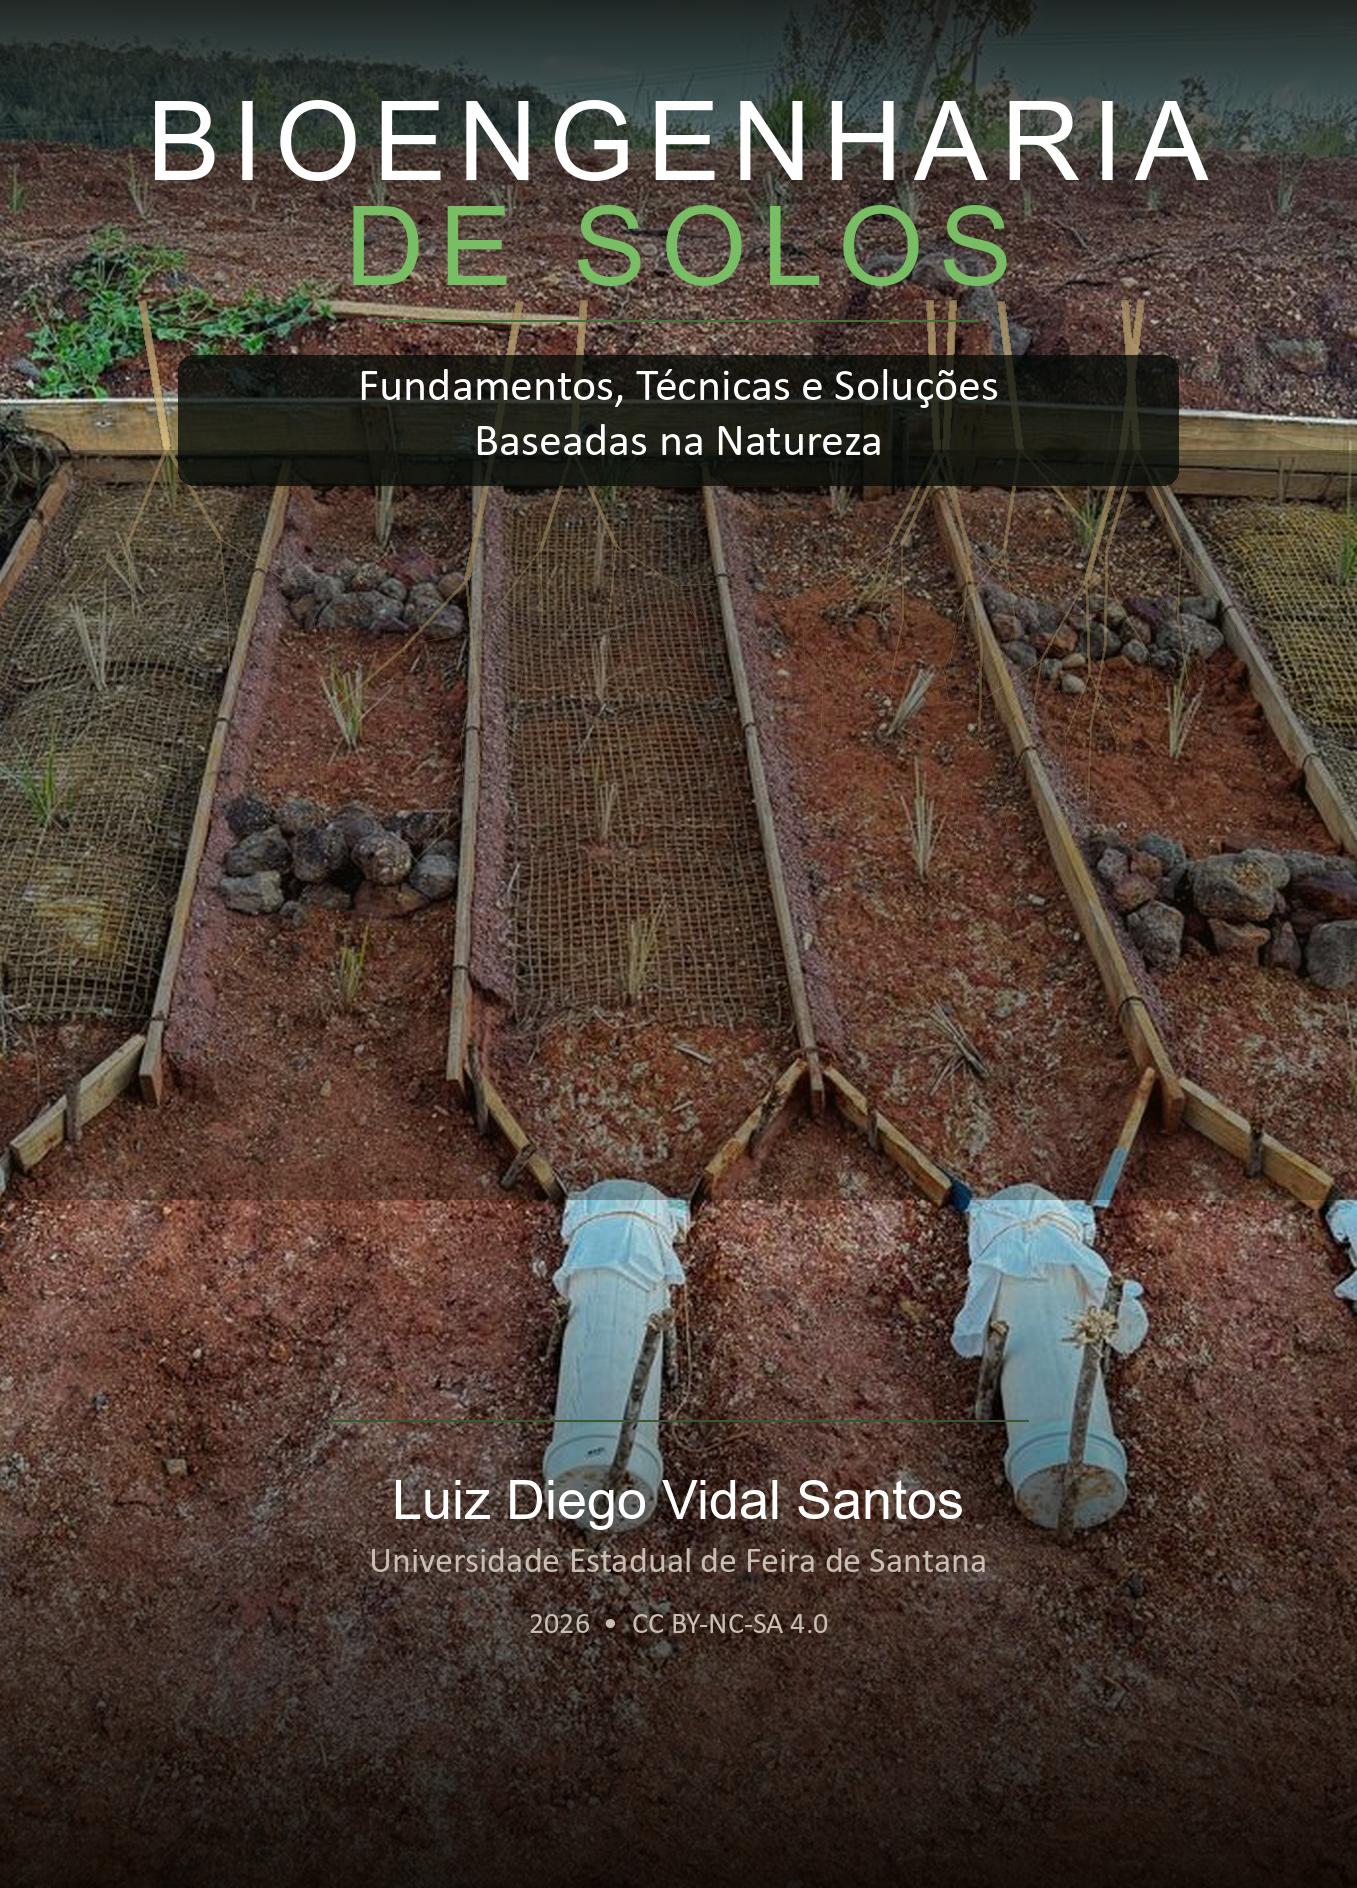
\includegraphics[width=\paperwidth,height=\paperheight]{img/capa_bioengenharia_de_solos.png}%
\restoregeometry%
\clearpage%
}
\makeatletter
\@ifpackageloaded{tcolorbox}{}{\usepackage[skins,breakable]{tcolorbox}}
\@ifpackageloaded{fontawesome5}{}{\usepackage{fontawesome5}}
\definecolor{quarto-callout-color}{HTML}{909090}
\definecolor{quarto-callout-note-color}{HTML}{0758E5}
\definecolor{quarto-callout-important-color}{HTML}{CC1914}
\definecolor{quarto-callout-warning-color}{HTML}{EB9113}
\definecolor{quarto-callout-tip-color}{HTML}{00A047}
\definecolor{quarto-callout-caution-color}{HTML}{FC5300}
\definecolor{quarto-callout-color-frame}{HTML}{acacac}
\definecolor{quarto-callout-note-color-frame}{HTML}{4582ec}
\definecolor{quarto-callout-important-color-frame}{HTML}{d9534f}
\definecolor{quarto-callout-warning-color-frame}{HTML}{f0ad4e}
\definecolor{quarto-callout-tip-color-frame}{HTML}{02b875}
\definecolor{quarto-callout-caution-color-frame}{HTML}{fd7e14}
\makeatother
\makeatletter
\@ifpackageloaded{bookmark}{}{\usepackage{bookmark}}
\makeatother
\makeatletter
\@ifpackageloaded{caption}{}{\usepackage{caption}}
\AtBeginDocument{%
\ifdefined\contentsname
  \renewcommand*\contentsname{Índice}
\else
  \newcommand\contentsname{Índice}
\fi
\ifdefined\listfigurename
  \renewcommand*\listfigurename{Lista de Figuras}
\else
  \newcommand\listfigurename{Lista de Figuras}
\fi
\ifdefined\listtablename
  \renewcommand*\listtablename{Lista de Tabelas}
\else
  \newcommand\listtablename{Lista de Tabelas}
\fi
\ifdefined\figurename
  \renewcommand*\figurename{Figura}
\else
  \newcommand\figurename{Figura}
\fi
\ifdefined\tablename
  \renewcommand*\tablename{Tabela}
\else
  \newcommand\tablename{Tabela}
\fi
}
\@ifpackageloaded{float}{}{\usepackage{float}}
\floatstyle{ruled}
\@ifundefined{c@chapter}{\newfloat{codelisting}{h}{lop}}{\newfloat{codelisting}{h}{lop}[chapter]}
\floatname{codelisting}{Listagem}
\newcommand*\listoflistings{\listof{codelisting}{Lista de Listagens}}
\makeatother
\makeatletter
\makeatother
\makeatletter
\@ifpackageloaded{caption}{}{\usepackage{caption}}
\@ifpackageloaded{subcaption}{}{\usepackage{subcaption}}
\makeatother
\usepackage{bookmark}
\IfFileExists{xurl.sty}{\usepackage{xurl}}{} % add URL line breaks if available
\urlstyle{same}
\hypersetup{
  pdftitle={Bioengenharia de Solos em Regiões Tropicais},
  pdfauthor={Luiz Diego Vidal Santos},
  pdflang={pt},
  colorlinks=true,
  linkcolor={Maroon},
  filecolor={Maroon},
  citecolor={Blue},
  urlcolor={Blue},
  pdfcreator={LaTeX via pandoc}}


\title{Bioengenharia de Solos em Regiões Tropicais}
\usepackage{etoolbox}
\makeatletter
\providecommand{\subtitle}[1]{% add subtitle to \maketitle
  \apptocmd{\@title}{\par {\large #1 \par}}{}{}
}
\makeatother
\subtitle{Fundamentos, Técnicas e Soluções Baseadas na Natureza}
\author{Luiz Diego Vidal Santos}
\date{15/02/2026}
\begin{document}
\frontmatter
\maketitle

\renewcommand*\contentsname{Índice}
{
\hypersetup{linkcolor=}
\setcounter{tocdepth}{2}
\tableofcontents
}

\mainmatter
\bookmarksetup{startatroot}

\chapter*{Sobre este livro}\label{sobre-este-livro}
\addcontentsline{toc}{chapter}{Sobre este livro}

\markboth{Sobre este livro}{Sobre este livro}

Este é o site do livro ``Bioengenharia de Solos em Regiões Tropicais:
Fundamentos, Técnicas e Soluções Baseadas na Natureza'', escrito por
\href{https://diegovidalcv.com.br/}{Luiz Diego Vidal Santos}.

A bioengenharia de solos combina princípios da engenharia, ecologia e
pedologia para estabilizar e recuperar solos degradados utilizando
materiais vivos e biodegradáveis. Em regiões tropicais, onde a
intensidade das chuvas, a profundidade do intemperismo e a fragilidade
dos solos impõem desafios únicos, as soluções baseadas na natureza (NBS)
surgem como alternativas sustentáveis, eficientes e de baixo custo.

Este livro apresenta de forma integrada os fundamentos pedológicos, as
técnicas construtivas e as inovações em materiais biodegradáveis
aplicados à conservação e recuperação de solos em ambientes tropicais.
Cada capítulo combina base teórica, equações de dimensionamento,
exemplos práticos e estudos de caso reais.

O conteúdo está organizado em quatro partes:

\begin{enumerate}
\def\labelenumi{\arabic{enumi}.}
\tightlist
\item
  Fundamentos --- Formação dos solos tropicais, intemperismo, processos
  erosivos e classificação de feições.
\item
  Técnicas de Bioengenharia --- Das paliçadas e bacias de captação aos
  gabiões vivos e paredes Krainer.
\item
  Geotêxteis e Inovação --- Geossintéticos, biotêxteis de fibras
  vegetais e biopolímeros superabsorventes.
\item
  Projeto e Integração --- Soluções baseadas na natureza e projeto
  integrador de bioengenharia.
\end{enumerate}

\section*{Para quem é}\label{para-quem-uxe9}
\addcontentsline{toc}{section}{Para quem é}

\markright{Para quem é}

\begin{itemize}
\tightlist
\item
  Estudantes de graduação e pós-graduação em Engenharia Agronômica,
  Ambiental, Civil e Florestal
\item
  Profissionais de conservação do solo e recuperação de áreas degradadas
\item
  Pesquisadores em soluções baseadas na natureza (NBS)
\item
  Gestores de bacias hidrográficas e planejamento territorial
\end{itemize}

\section*{Como citar}\label{como-citar}
\addcontentsline{toc}{section}{Como citar}

\markright{Como citar}

\begin{quote}
Santos, L. D. V. (2026). \emph{Bioengenharia de Solos em Regiões
Tropicais: Fundamentos, Técnicas e Soluções Baseadas na Natureza}.
Disponível em:
\url{https://diegovidalcv.com.br/books/bioengenharia-solos/}
\end{quote}

\section*{Licença}\label{licenuxe7a}
\addcontentsline{toc}{section}{Licença}

\markright{Licença}

Este livro é disponibilizado sob licença
\href{https://creativecommons.org/licenses/by-nc-sa/4.0/}{Creative
Commons Atribuição-NãoComercial-CompartilhaIgual 4.0 Internacional (CC
BY-NC-SA 4.0)}.

\bookmarksetup{startatroot}

\chapter{}\label{section}

\# Prefácio \{.unnumbered\}

A erosão do solo é um dos maiores desafios ambientais do século XXI.
Estima-se que 24 bilhões de toneladas de solo fértil sejam perdidas
anualmente em todo o mundo, com consequências diretas na segurança
alimentar, nos recursos hídricos e na biodiversidade. Em regiões
tropicais, a combinação de chuvas intensas, solos profundamente
intemperizados e pressão antrópica agrava esse cenário.

A bioengenharia de solos (entendida como o uso de materiais vivos e
biodegradáveis combinados a técnicas de engenharia) oferece uma resposta
a esse desafio. Diferentemente das soluções exclusivamente estruturais,
a bioengenharia busca a transição progressiva de uma função mecânica
artificial para uma função ecológica natural, de modo que, à medida que
os materiais se degradam, as raízes das plantas assumem o papel de
sustentação do solo.

Este livro nasceu da experiência acumulada em mais de uma década de
pesquisa e extensão no Baixo São Francisco (SE/AL) e nos Tabuleiros
Costeiros do Nordeste brasileiro. A convivência com agricultores
familiares, comunidades ribeirinhas e técnicos de campo me ensinou que
as melhores soluções são aquelas que combinam rigor científico,
viabilidade econômica e apropriação social.

Ao longo dos capítulos, o leitor encontrará equações e modelos de
dimensionamento aplicáveis a condições tropicais, estudos de caso de
campo com dados reais de monitoramento, comparativos de custo entre
soluções convencionais e baseadas na natureza, e inovações tecnológicas
em materiais biodegradáveis protegidos por patentes.

Agradeço aos colegas do grupo de pesquisa PLANeT-Inova (UEFS), do
Gerenciamento Hidroambiental do Baixo São Francisco (UFS) e do Manejo de
Solos e Sustentabilidade (UFS) pelas colaborações que enriqueceram este
trabalho.

\textbf{Luiz Diego Vidal Santos}\\
Feira de Santana, Bahia\\
Fevereiro de 2026

\part{Parte I --- Fundamentos}

\chapter{O que é Bioengenharia de
Solos?}\label{o-que-uxe9-bioengenharia-de-solos}

\# Introdução à Bioengenharia de Solos \{\#sec-introducao\}

A bioengenharia de solos (\emph{soil bioengineering}) é uma disciplina
que combina princípios da engenharia civil, ecologia e ciência do solo
para projetar, construir e manter estruturas de estabilização e proteção
do solo utilizando materiais vivos (plantas, raízes, estacas) combinados
ou não a materiais inertes biodegradáveis (fibras naturais, madeira,
bambu).

O conceito difere da engenharia convencional em um aspecto fundamental.
Enquanto as estruturas de concreto e aço são projetadas para resistir
indefinidamente ao intemperismo, as estruturas de bioengenharia são
projetadas para uma transição funcional, na qual a resistência mecânica
inicial (fornecida por materiais construtivos) é progressivamente
transferida para o sistema radicular das plantas à medida que estas se
estabelecem (Figura~\ref{fig-transicao}).

\begin{figure}

\centering{

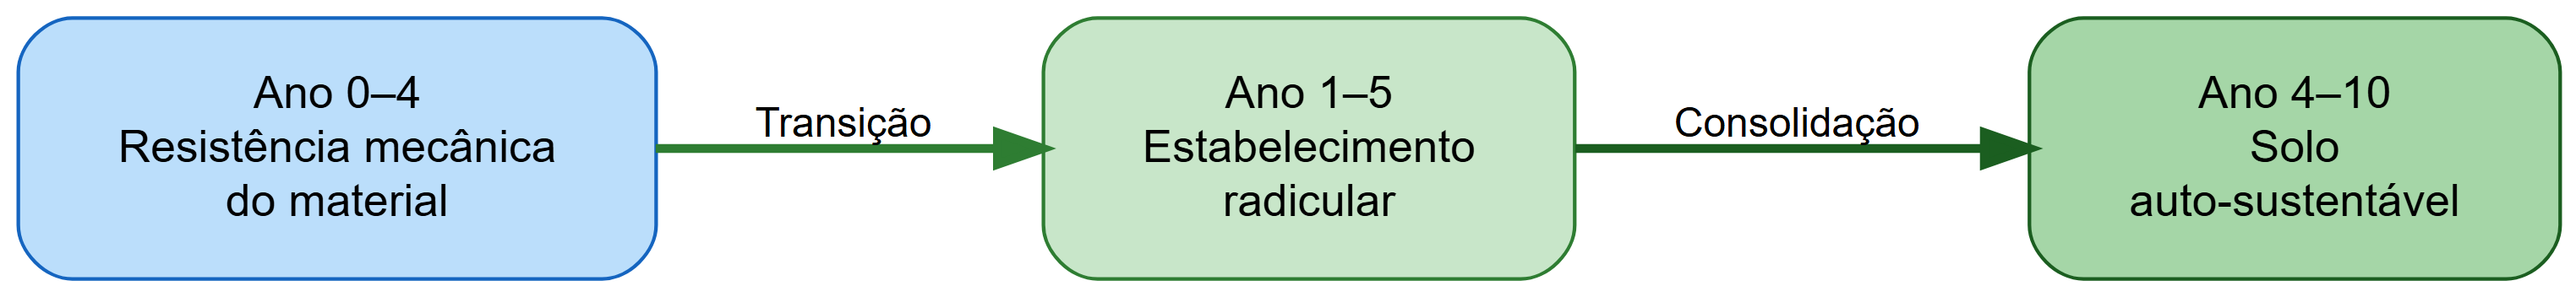
\includegraphics[width=7in,height=3.5in]{capitulos/01-introducao_files/figure-latex/dot-figure-1.png}

}

\caption{\label{fig-transicao}Esquema conceitual da transição entre a
função mecânica dos materiais construtivos e a função ecológica do
sistema radicular.}

\end{figure}%

\section{Bioengenharia vs.~Engenharia
Convencional}\label{bioengenharia-vs.-engenharia-convencional}

\begin{longtable}[]{@{}
  >{\raggedright\arraybackslash}p{(\linewidth - 4\tabcolsep) * \real{0.1786}}
  >{\raggedright\arraybackslash}p{(\linewidth - 4\tabcolsep) * \real{0.4286}}
  >{\raggedright\arraybackslash}p{(\linewidth - 4\tabcolsep) * \real{0.3929}}@{}}
\caption{Comparativo entre engenharia convencional e bioengenharia de
solos.}\label{tbl-comparativo}\tabularnewline
\toprule\noalign{}
\begin{minipage}[b]{\linewidth}\raggedright
Critério
\end{minipage} & \begin{minipage}[b]{\linewidth}\raggedright
Engenharia Convencional
\end{minipage} & \begin{minipage}[b]{\linewidth}\raggedright
Bioengenharia de Solos
\end{minipage} \\
\midrule\noalign{}
\endfirsthead
\toprule\noalign{}
\begin{minipage}[b]{\linewidth}\raggedright
Critério
\end{minipage} & \begin{minipage}[b]{\linewidth}\raggedright
Engenharia Convencional
\end{minipage} & \begin{minipage}[b]{\linewidth}\raggedright
Bioengenharia de Solos
\end{minipage} \\
\midrule\noalign{}
\endhead
\bottomrule\noalign{}
\endlastfoot
Material principal & Concreto, aço, gabião metálico & Plantas, fibras,
madeira, bambu \\
Durabilidade do material & Décadas a séculos & 2--10 anos
(biodegradável) \\
Função ao longo do tempo & Constante (ou degradante) & Crescente
(sistema vivo) \\
Custo inicial & Alto & Moderado a baixo \\
Custo de manutenção & Médio & Baixo \\
Impacto paisagístico & Negativo & Positivo \\
Serviços ecossistêmicos & Nenhum & Múltiplos \\
Emissão de CO₂ & Alta & Sequestro de C \\
\end{longtable}

\section{Histórico}\label{histuxf3rico}

A bioengenharia de solos tem raízes milenares. Na China, há registros de
uso de fascinas de bambu para contenção de margens de rios datados de
mais de 2.000 anos. Na Europa, técnicas de estabilização com estacas
vivas de salgueiro (\emph{Salix} spp.) são documentadas desde o século
XVIII (Schiechtl, 1980).

O desenvolvimento moderno da disciplina ocorreu na segunda metade do
século XX, com contribuições fundamentais de Hugo M. Schiechtl
(Áustria), que sistematizou as técnicas de \emph{Ingenieurbiologie} ao
publicar o primeiro manual técnico em 1973. Na América do Norte, Donald
H. Gray e Robbin B. Sotir consolidaram o campo com o clássico
\emph{Biotechnical and Soil Bioengineering Slope Stabilization} (Gray \&
Sotir, 1996). No Brasil, Fabrício J. Sutili e Miguel A. Durlo foram
pioneiros na adaptação das técnicas europeias ao contexto subtropical
brasileiro (Durlo \& Sutili, 2005; Sutili, 2004).

\section{Contexto Tropical}\label{contexto-tropical}

Em regiões tropicais, a bioengenharia enfrenta desafios e oportunidades
particulares:

\begin{tcolorbox}[enhanced jigsaw, leftrule=.75mm, colframe=quarto-callout-important-color-frame, colback=white, bottomrule=.15mm, opacityback=0, colbacktitle=quarto-callout-important-color!10!white, breakable, bottomtitle=1mm, opacitybacktitle=0.6, title=\textcolor{quarto-callout-important-color}{\faExclamation}\hspace{0.5em}{Desafios tropicais}, titlerule=0mm, toprule=.15mm, toptitle=1mm, rightrule=.15mm, left=2mm, arc=.35mm, coltitle=black]

As regiões tropicais impõem condições severas à bioengenharia. A
intensidade pluviométrica, com chuvas concentradas cuja erosividade é
3--5× maior que em zonas temperadas, exige estruturas com alta
capacidade de dissipação de energia. O intemperismo profundo gera perfis
de solo com 10--30 m de manto de alteração, nos quais predominam argilas
1:1 (caulinita) com baixa CTC (solos lateríticos). Soma-se a isso a
necessidade de seleção criteriosa de espécies nativas adaptadas, dada a
elevada biodiversidade das paisagens tropicais.

\end{tcolorbox}

\begin{tcolorbox}[enhanced jigsaw, leftrule=.75mm, colframe=quarto-callout-tip-color-frame, colback=white, bottomrule=.15mm, opacityback=0, colbacktitle=quarto-callout-tip-color!10!white, breakable, bottomtitle=1mm, opacitybacktitle=0.6, title=\textcolor{quarto-callout-tip-color}{\faLightbulb}\hspace{0.5em}{Oportunidades tropicais}, titlerule=0mm, toprule=.15mm, toptitle=1mm, rightrule=.15mm, left=2mm, arc=.35mm, coltitle=black]

Em contrapartida, as condições tropicais oferecem vantagens expressivas.
As taxas de rebrota vegetal são 2--4× maiores que em zonas temperadas,
acelerando a transição funcional. A disponibilidade de fibras naturais
(sisal, coco, taboa \emph{Typha}, bananeira e rami) e de materiais
locais (bambu, pedras e madeiras de rápido crescimento) reduz custos,
enquanto a viabilidade econômica de mão de obra intensiva favorece
técnicas de execução manual.

\end{tcolorbox}

\section{Estrutura deste Livro}\label{estrutura-deste-livro}

Este livro está organizado em quatro partes:

A Parte I (Fundamentos) apresenta a base científica necessária,
incluindo formação dos solos tropicais, processos de intemperismo,
mecanismos erosivos e classificação de feições. A Parte II (Técnicas de
Bioengenharia) detalha as técnicas construtivas, do mais simples ao mais
complexo, com equações de dimensionamento e exemplos práticos. A Parte
III (Geotêxteis e Inovação) aborda geossintéticos convencionais,
biotêxteis de fibras vegetais e biopolímeros superabsorventes, incluindo
patentes desenvolvidas pelo autor. Por fim, a Parte IV (Projeto e
Integração) apresenta o conceito de soluções baseadas na natureza (NBS)
e um roteiro para projeto integrador de bioengenharia.

\chapter{O Solo como Sistema Aberto}\label{o-solo-como-sistema-aberto}

\# Solos Tropicais: Formação e Propriedades \{\#sec-solos-tropicais\}

Antes de projetar qualquer intervenção de bioengenharia, é indispensável
compreender o material sobre o qual se trabalha. O solo não é uma massa
inerte de partículas minerais; trata-se de um sistema aberto
termodinâmico que troca continuamente matéria e energia com a atmosfera,
a biosfera, a hidrosfera e a litosfera. Imagine o solo como uma
``fábrica viva'' que recebe água da chuva, gases da atmosfera, resíduos
orgânicos e libera sedimentos dissolvidos, gases (como CO₂) e nutrientes
em solução.

Em regiões tropicais, a intensidade dessas trocas é amplificada pela
temperatura elevada (média anual \textgreater{} 20 °C) e pela abundância
de água (precipitação acumulada frequentemente superior a 1.200 mm/ano),
resultando em solos profundamente intemperizados e com características
únicas. Essa combinação confere aos solos tropicais um conjunto de
propriedades que os distingue radicalmente dos solos de regiões
temperadas, com implicações diretas para o projeto de estruturas de
bioengenharia.

\section{A Equação de Jenny}\label{a-equauxe7uxe3o-de-jenny}

A formação do solo é um fenômeno complexo cuja compreensão exige
considerar múltiplos fatores atuando simultaneamente. A equação fatorial
proposta por Jenny (1941) sintetiza esse entendimento, conforme
ilustrado na Figura~\ref{fig-jenny}.

\begin{figure}

\centering{


\includegraphics[width=0.8\linewidth,height=\textheight,keepaspectratio]{capitulos/../img/jenny_fatores.png}

}

\caption{\label{fig-jenny}Fatores de formação do solo segundo Jenny
(1941): Clima, Organismos, Relevo, Material de Origem e Tempo.}

\end{figure}%

Matematicamente, qualquer propriedade do solo (\(S\)) pode ser expressa
como função dos cinco fatores de formação:

\[
S = f(cl, o, r, p, t, \ldots)
\]

onde \(S\) é a propriedade do solo (textura, cor, CTC, profundidade,
etc.), \(cl\) representa o clima (precipitação e temperatura, que
controlam a intensidade do intemperismo), \(o\) corresponde aos
organismos (vegetação, fauna do solo, microrganismos que reciclam
matéria orgânica), \(r\) é o relevo (que governa o escoamento da água e
a redistribuição de sedimentos ao longo da encosta), \(p\) indica o
material de origem (a rocha-mãe fornece os minerais primários a partir
dos quais o solo é formado) e \(t\) é o tempo (solos tropicais bem
desenvolvidos possuem idades da ordem de milhões de anos). O termo
\(\ldots\) reconhece fatores adicionais, sobretudo a ação antrópica.

Na prática, a equação de Jenny ensina que dois solos formados sob o
mesmo clima, relevo, material de origem, biota e tempo terão
propriedades semelhantes. Por isso, quando se identifica, por exemplo,
um Latossolo Vermelho em duas regiões distintas do Cerrado brasileiro,
espera-se comportamento geotécnico e erodibilidade comparáveis, o que
permite transferir experiências de bioengenharia entre localidades
análogas.

\begin{tcolorbox}[enhanced jigsaw, leftrule=.75mm, colframe=quarto-callout-note-color-frame, colback=white, bottomrule=.15mm, opacityback=0, colbacktitle=quarto-callout-note-color!10!white, breakable, bottomtitle=1mm, opacitybacktitle=0.6, title=\textcolor{quarto-callout-note-color}{\faInfo}\hspace{0.5em}{ClORPT}, titlerule=0mm, toprule=.15mm, toptitle=1mm, rightrule=.15mm, left=2mm, arc=.35mm, coltitle=black]

O acrônimo ClORPT é uma forma didática de memorizar os fatores de
formação do solo: Clima, Organismos, Relevo, Parent material (material
de origem) e Tempo. Nos trópicos, o clima (especialmente a precipitação)
e o tempo são os fatores dominantes, o que explica o intemperismo
avançado mesmo sobre diferentes tipos de rocha.

\end{tcolorbox}

\section{Reator Biogeoquímico}\label{reator-biogeoquuxedmico}

Para entender por que os solos tropicais são tão diferentes dos solos de
regiões frias, é útil pensar no solo como um reator biogeoquímico,
conforme esquematizado na Figura~\ref{fig-reator}.

\begin{figure}

\centering{

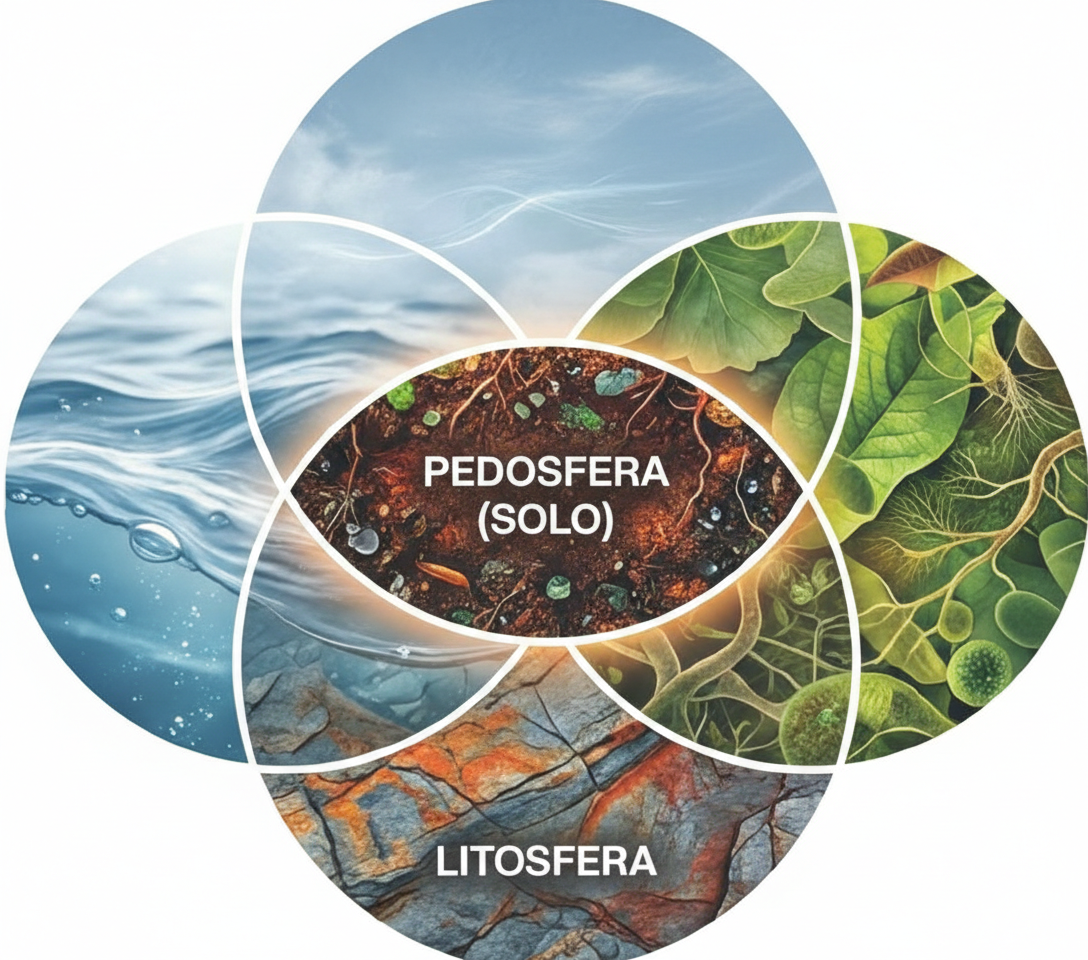
\includegraphics[width=0.8\linewidth,height=\textheight,keepaspectratio]{capitulos/../img/reator_biogeoquimico.png}

}

\caption{\label{fig-reator}O solo como reator biogeoquímico: processos
simultâneos de adição, remoção, transformação e translocação.}

\end{figure}%

Neste reator, quatro processos fundamentais operam simultaneamente. O
processo de adição incorpora matéria orgânica pela deposição de
serrapilheira, poeira atmosférica e solutos trazidos pela chuva. O
processo de remoção retira material por lixiviação (percolação de água
que dissolve e carrega íons), erosão superficial e extração por
colheitas agrícolas. A transformação converte minerais primários em
minerais secundários (argilas e óxidos) por reações de hidrólise,
oxidação e redução, além de decompor matéria orgânica em húmus. Por fim,
a translocação redistribui materiais internamente, movendo argilas de
horizontes superiores para inferiores (fenômeno chamado
eluviação/iluviação) e revolvendo o solo por atividade de organismos
(bioturbação por minhocas, cupins e formigas).

Em regiões tropicais, as taxas de transformação são significativamente
maiores devido à temperatura e umidade elevadas. Cada aumento de 10 °C
na temperatura aproximadamente duplica a velocidade das reações químicas
(Lei de Arrhenius). Isso resulta em três consequências fundamentais para
a bioengenharia: a decomposição rápida da matéria orgânica (meia-vida
inferior a 5 anos, contra 15--25 anos em zonas temperadas), a alta taxa
de neoformação de argilas cauliníticas (minerais de baixa atividade) e a
concentração residual de óxidos de ferro e alumínio pelo processo de
laterização (que confere as cores vermelhas e amarelas características).

\section{Perfil do Solo Tropical}\label{perfil-do-solo-tropical}

Um conceito essencial para quem projeta intervenções de bioengenharia é
o de perfil do solo, que consiste na sequência vertical de camadas
(chamadas horizontes) que se desenvolvem desde a superfície até a
rocha-mãe inalterada. Cada horizonte possui propriedades distintas de
cor, textura, estrutura e composição química, e essas diferenças
determinam como a água se infiltra, como as raízes se desenvolvem e onde
o solo é mais suscetível a rupturas.

A Figura~\ref{fig-perfil} apresenta um perfil típico de solo tropical,
onde é possível observar a transição gradual desde a matéria orgânica
superficial até o material parental inalterado em profundidade.

\begin{figure}

\centering{

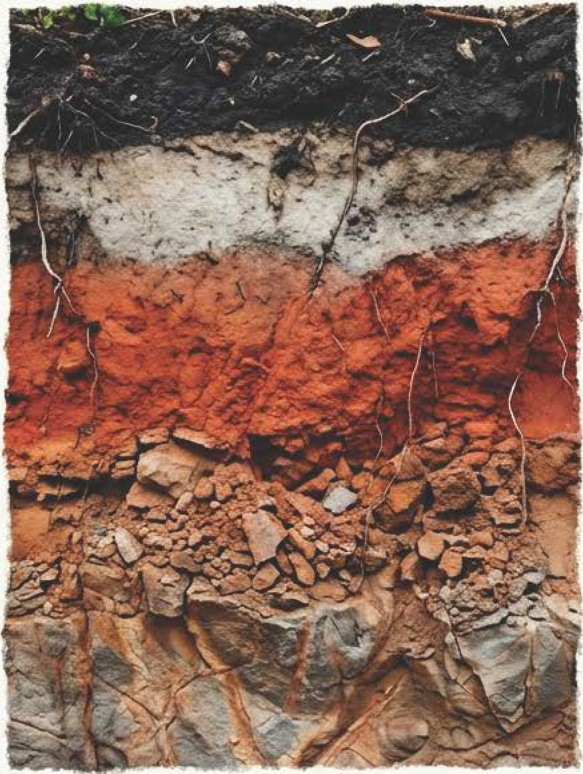
\includegraphics[width=0.7\linewidth,height=\textheight,keepaspectratio]{capitulos/../img/perfil_solo.jpg}

}

\caption{\label{fig-perfil}Perfil de solo tropical com horizontes bem
definidos, mostrando a transição da matéria orgânica superficial até a
rocha-mãe.}

\end{figure}%

A representação esquemática dos horizontes e suas transições é detalhada
na Figura~\ref{fig-horizontes}, que permite visualizar as nomenclaturas
padronizadas utilizadas em levantamentos de solo.

\begin{figure}

\centering{

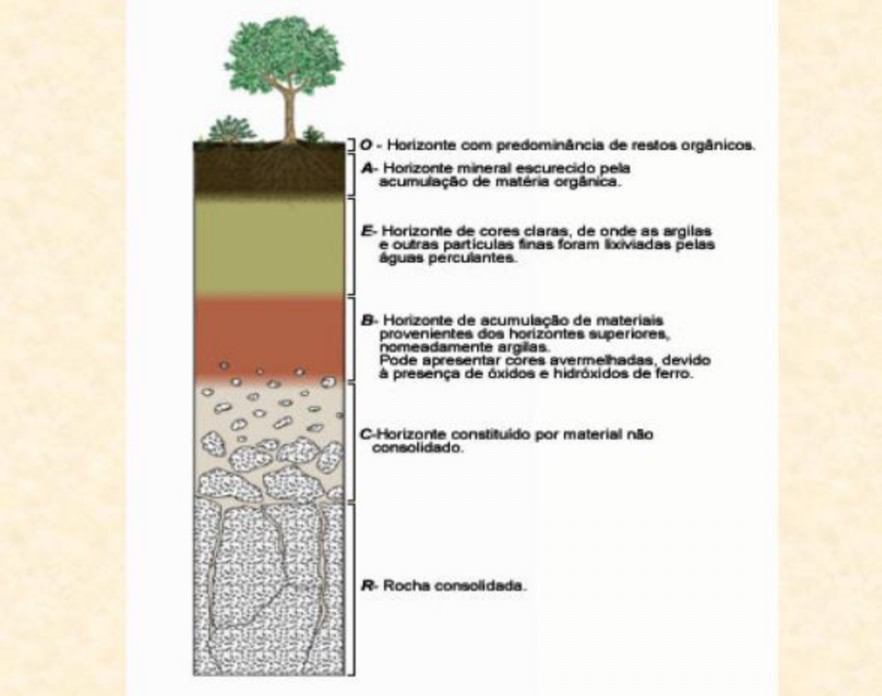
\includegraphics[width=0.7\linewidth,height=\textheight,keepaspectratio]{capitulos/../img/horizontes_solo.jpg}

}

\caption{\label{fig-horizontes}Representação esquemática dos horizontes
do solo e suas transições.}

\end{figure}%

O perfil típico de um solo tropical bem drenado apresenta a sequência
descrita na Tabela~\ref{tbl-perfil}. Note que a espessura total do
perfil pode ultrapassar 10 metros em Latossolos, enquanto em Neossolos
Litólicos (solos rasos de encostas íngremes) pode ser inferior a 50 cm,
condição que exige estratégias de bioengenharia completamente distintas.

\begin{longtable}[]{@{}
  >{\raggedright\arraybackslash}p{(\linewidth - 4\tabcolsep) * \real{0.2391}}
  >{\raggedright\arraybackslash}p{(\linewidth - 4\tabcolsep) * \real{0.4130}}
  >{\raggedright\arraybackslash}p{(\linewidth - 4\tabcolsep) * \real{0.3478}}@{}}
\caption{Perfil esquemático de um solo tropical profundo
(Latossolo).}\label{tbl-perfil}\tabularnewline
\toprule\noalign{}
\begin{minipage}[b]{\linewidth}\raggedright
Horizonte
\end{minipage} & \begin{minipage}[b]{\linewidth}\raggedright
Profundidade típica
\end{minipage} & \begin{minipage}[b]{\linewidth}\raggedright
Características
\end{minipage} \\
\midrule\noalign{}
\endfirsthead
\toprule\noalign{}
\begin{minipage}[b]{\linewidth}\raggedright
Horizonte
\end{minipage} & \begin{minipage}[b]{\linewidth}\raggedright
Profundidade típica
\end{minipage} & \begin{minipage}[b]{\linewidth}\raggedright
Características
\end{minipage} \\
\midrule\noalign{}
\endhead
\bottomrule\noalign{}
\endlastfoot
O & 0--5 cm & Serrapilheira em decomposição; protege contra o impacto
direto das gotas de chuva \\
A & 5--30 cm & Matéria orgânica humificada, cor escura; zona de maior
atividade biológica e radicular \\
B & 30--200+ cm & Argilas cauliníticas, óxidos de Fe/Al, cor amarela a
vermelha; horizonte diagnóstico \\
C & 200--1000+ cm & Saprolito (rocha parcialmente intemperizada);
preserva estrutura da rocha original \\
R & \textgreater{} 10 m & Rocha-mãe inalterada \\
\end{longtable}

\begin{figure}

\centering{

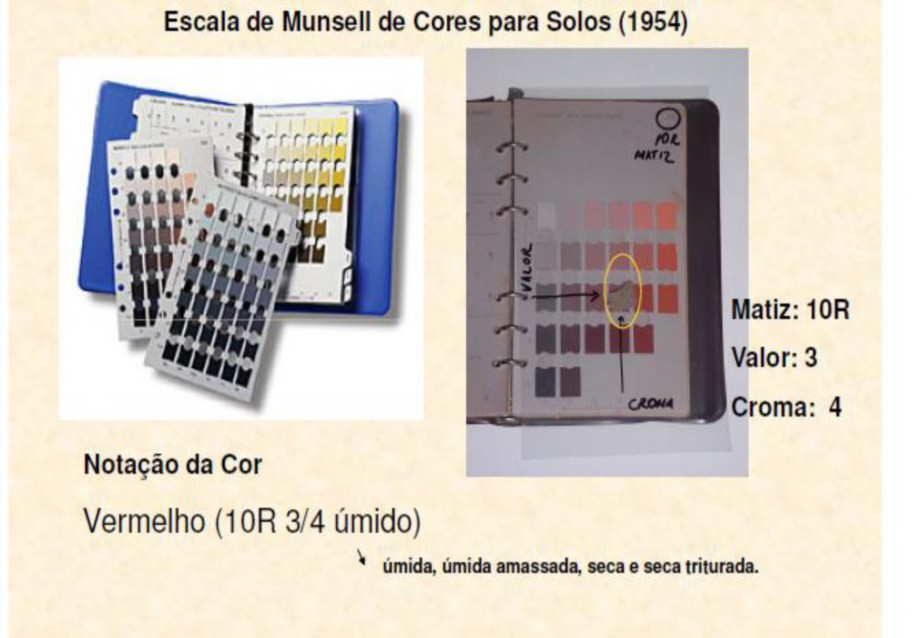
\includegraphics[width=0.7\linewidth,height=\textheight,keepaspectratio]{capitulos/../img/cores_munsell.jpg}

}

\caption{\label{fig-munsell}Carta de cores de Munsell --- ferramenta
padrão para determinação objetiva da cor do solo em campo, utilizada na
descrição morfológica de horizontes.}

\end{figure}%

Para a bioengenharia, a distinção entre horizontes é crítica. O
horizonte A, rico em matéria orgânica e raízes, é o que se busca
preservar ou reconstituir. O horizonte B, frequentemente espesso e
laterizado, pode apresentar coesão aparente (estável quando seco, mas
colapsável quando saturado), o que torna fundamental o controle da
drenagem superficial e subsuperficial. Quando a erosão atinge o
horizonte C ou mesmo o R, a recuperação é muito mais complexa e onerosa.

\section{Propriedades-chave para
Bioengenharia}\label{propriedades-chave-para-bioengenharia}

\subsection{Textura e Estrutura}\label{textura-e-estrutura}

A textura do solo (proporção relativa de areia, silte e argila) é uma
das propriedades mais importantes para o projeto de bioengenharia, pois
influencia diretamente a erodibilidade, a capacidade de infiltração e a
resistência ao cisalhamento. A classificação textural é realizada com
auxílio do triângulo textural, apresentado na
Figura~\ref{fig-triangulo}.

\begin{figure}

\centering{

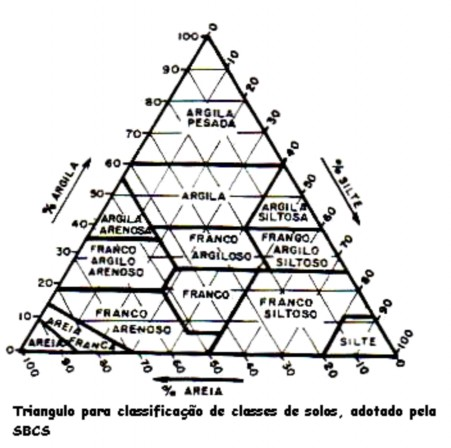
\includegraphics[width=0.65\linewidth,height=\textheight,keepaspectratio]{capitulos/../img/triangulo_textural.jpg}

}

\caption{\label{fig-triangulo}Triângulo textural para classificação de
solos segundo a proporção de areia, silte e argila.}

\end{figure}%

Para interpretar o triângulo textural, localiza-se o ponto de interseção
entre as três frações granulométricas (obtidas por ensaio de
granulometria em laboratório), e a classe textural resultante orienta as
decisões de projeto. Os solos arenosos (fração areia \textgreater{}
70\%) apresentam alta taxa de infiltração (\textgreater{} 50 mm/h),
porém baixa coesão entre partículas, tornando-os altamente susceptíveis
ao desenvolvimento de ravinas por escoamento concentrado. Os solos
argilosos (fração argila \textgreater{} 35\%), em contrapartida, possuem
baixa taxa de infiltração (\textless{} 10 mm/h) e alta coesão quando
secos, mas oferecem risco de deslizamento quando saturados, pois a água
nos poros gera poropressão positiva que reduz a tensão efetiva. Já os
solos siltosos são considerados os mais erodíveis, pois combinam baixa
coesão entre partículas com baixa permeabilidade, o que gera escoamento
superficial intenso capaz de transportar grandes volumes de sedimento.

\subsection{Fator de Erodibilidade (K)}\label{fator-de-erodibilidade-k}

Para quantificar objetivamente a susceptibilidade intrínseca de um solo
à erosão (independentemente da chuva, do relevo ou do uso do solo),
utiliza-se o fator \(K\) da RUSLE (Renard et al., 1997):

\[
K = 2{,}1 \times 10^{-4} \cdot M^{1{,}14} \cdot (12 - a) + 3{,}25 \cdot (b - 2) + 2{,}5 \cdot (c - 3) \div 100
\]

onde \(M\) representa o produto
\((\% \text{silte} + \% \text{areia fina}) \times (100 - \% \text{argila})\),
\(a\) corresponde ao teor de matéria orgânica (\%), \(b\) indica a
classe de estrutura do solo (1--4, sendo 1 = granular muito fina e 4 =
blocos, laminar ou maciça) e \(c\) refere-se à classe de permeabilidade
(1--6, sendo 1 = rápida e 6 = muito lenta).

Em termos práticos, solos com alto teor de silte e areia fina (elevado
\(M\)) e baixo teor de matéria orgânica (baixo \(a\)) resultam em
valores de \(K\) elevados (alta erodibilidade), o que demanda maior
proteção superficial pelas técnicas de bioengenharia. Solos tropicais
laterizados tendem a apresentar \(K\) moderado (0,02--0,04 t h MJ⁻¹
mm⁻¹) graças à microagregação conferida pelos óxidos de ferro, apesar do
altíssimo teor de argila.

\subsection{Resistência ao
Cisalhamento}\label{resistuxeancia-ao-cisalhamento}

A estabilidade de encostas e taludes depende fundamentalmente da
resistência ao cisalhamento (\(\tau\)) do solo, descrita pelo critério
de Mohr-Coulomb:

\[
\tau = c' + (\sigma - u) \tan \phi'
\]

onde \(c'\) é a coesão efetiva (força de ligação entre partículas),
\(\sigma\) é a tensão normal total (peso do solo acima do plano de
ruptura), \(u\) é a poropressão (pressão exercida pela água nos poros,
que ``empurra'' as partículas e reduz o atrito entre elas) e \(\phi'\) é
o ângulo de atrito interno efetivo (resistência ao deslizamento entre
partículas). Quando a poropressão (\(u\)) aumenta (por exemplo, durante
chuvas intensas que saturam o solo), a tensão efetiva \((\sigma - u)\)
diminui, a resistência ao cisalhamento cai e o talude pode romper. Esse
é o mecanismo fundamental dos deslizamentos em encostas tropicais.

A bioengenharia intervém diretamente nessa equação. A presença de raízes
aumenta a coesão do solo, adicionando um termo \(c_r\) (coesão
radicular) à coesão efetiva. O incremento de coesão radicular pode ser
estimado pelo modelo de Wu-Waldron:

\[
c_r = t_R \cdot \frac{A_r}{A} \cdot (\sin \theta + \cos \theta \cdot \tan \phi')
\]

onde \(t_R\) é a resistência à tração das raízes (quanto uma raiz
individual resiste antes de romper, medida em kPa), \(A_r/A\) é a razão
de área radicular (proporção da seção transversal do solo ocupada por
raízes) e \(\theta\) é o ângulo de distorção das raízes em relação ao
plano de ruptura. Dessa forma, quanto maior a densidade de raízes e
quanto mais resistentes elas forem, maior será o incremento de coesão e,
portanto, maior a estabilidade do talude.

\begin{tcolorbox}[enhanced jigsaw, leftrule=.75mm, colframe=quarto-callout-tip-color-frame, colback=white, bottomrule=.15mm, opacityback=0, colbacktitle=quarto-callout-tip-color!10!white, breakable, bottomtitle=1mm, opacitybacktitle=0.6, title=\textcolor{quarto-callout-tip-color}{\faLightbulb}\hspace{0.5em}{Valores típicos}, titlerule=0mm, toprule=.15mm, toptitle=1mm, rightrule=.15mm, left=2mm, arc=.35mm, coltitle=black]

Em solos tropicais com vegetação herbácea estabelecida (como gramíneas
Vetiver ou Brachiaria), o incremento \(c_r\) varia tipicamente de 5 a 25
kPa, podendo alcançar 40 kPa em solos com sistema radicular arbóreo
denso. Para contexto, uma coesão de 10 kPa já pode significar a
diferença entre um talude estável e um deslizamento em encostas com
inclinações entre 30° e 45°.

\end{tcolorbox}

\subsection{Condutividade Hidráulica}\label{condutividade-hidruxe1ulica}

A condutividade hidráulica saturada (\(K_s\)) é uma propriedade
fundamental para o dimensionamento de sistemas de drenagem em projetos
de bioengenharia, pois governa a taxa de infiltração de água no solo e a
velocidade de dissipação de poropressões em taludes. Em solos tropicais,
\(K_s\) apresenta comportamento paradoxal em relação à textura,
especialmente nos Latossolos, onde a microagregação por óxidos de ferro
confere permeabilidade elevada a solos com mais de 60\% de argila
(comportamento pseudo-arenoso). A determinação em campo é realizada por
ensaio de infiltração com permeâmetro de Guelph ou infiltrômetro de
duplo anel (ABNT NBR 7229), e em laboratório por permeâmetro de carga
constante ou variável conforme NBR 14545.

A Tabela~\ref{tbl-ks} apresenta valores típicos de \(K_s\) para as
principais classes de solos tropicais brasileiros, obtidos a partir de
compilação de ensaios publicados na literatura nacional. Esses valores
orientam o dimensionamento preliminar de geodrenos (ver
\textbf{?@sec-biotexteis}), bacias de captação (ver
\textbf{?@sec-bacias-captacao}) e canaletas verdes (ver
\textbf{?@sec-canaleta-verde}), devendo ser confirmados por ensaios in
situ na fase de projeto executivo.

\begin{longtable}[]{@{}
  >{\raggedright\arraybackslash}p{(\linewidth - 6\tabcolsep) * \real{0.1613}}
  >{\raggedright\arraybackslash}p{(\linewidth - 6\tabcolsep) * \real{0.2258}}
  >{\raggedright\arraybackslash}p{(\linewidth - 6\tabcolsep) * \real{0.2796}}
  >{\raggedright\arraybackslash}p{(\linewidth - 6\tabcolsep) * \real{0.3333}}@{}}
\caption{Condutividade hidráulica saturada típica para solos tropicais
brasileiros e implicações para
bioengenharia.}\label{tbl-ks}\tabularnewline
\toprule\noalign{}
\begin{minipage}[b]{\linewidth}\raggedright
Classe de solo
\end{minipage} & \begin{minipage}[b]{\linewidth}\raggedright
\(K_s\) típico (mm/h)
\end{minipage} & \begin{minipage}[b]{\linewidth}\raggedright
Comportamento hidráulico
\end{minipage} & \begin{minipage}[b]{\linewidth}\raggedright
Implicação para bioengenharia
\end{minipage} \\
\midrule\noalign{}
\endfirsthead
\toprule\noalign{}
\begin{minipage}[b]{\linewidth}\raggedright
Classe de solo
\end{minipage} & \begin{minipage}[b]{\linewidth}\raggedright
\(K_s\) típico (mm/h)
\end{minipage} & \begin{minipage}[b]{\linewidth}\raggedright
Comportamento hidráulico
\end{minipage} & \begin{minipage}[b]{\linewidth}\raggedright
Implicação para bioengenharia
\end{minipage} \\
\midrule\noalign{}
\endhead
\bottomrule\noalign{}
\endlastfoot
Latossolo argiloso (microagregado) & 50--200 & Rápida infiltração apesar
do alto teor de argila & Drenagem natural eficiente, risco de erosão
interna em descontinuidades \\
Latossolo arenoso & 100--500 & Muito permeável & Risco de percolação sob
paliçadas, exige vedação de base \\
Argissolo (horizonte Bt) & 1--15 & Baixa permeabilidade no horizonte Bt
& Gera lençol suspenso, essencial drenar a interface A/Bt \\
Plintossolo (petroplintita) & 0,1--5 & Quase impermeável quando
endurecido & Exige drenagem superficial agressiva, limita
enraizamento \\
Cambissolo & 10--80 & Variável conforme maturidade & Investigação local
obrigatória \\
Gleissolo (saturado) & 0,5--10 & Saturação permanente & Exige espécies
tolerantes a anaerobiose \\
Neossolo Quartzarênico & 200--800 & Extremamente permeável & Baixa
retenção hídrica, Bio-SAP recomendado (\textbf{?@sec-biopolimeros}) \\
\end{longtable}

A relação entre \(K_s\) e a intensidade da chuva de projeto (\(i\))
determina o mecanismo de geração de escoamento superficial. Quando
\(i > K_s\) (escoamento hortoniano), a precipitação excedente forma
escoamento superficial imediatamente, situação comum em Argissolos e
Plintossolos com horizonte de impedimento. Quando \(i < K_s\)
(escoamento por saturação), o solo infiltra toda a chuva até que a
capacidade de armazenamento se esgote, gerando escoamento apenas quando
o perfil satura por acúmulo progressivo, mecanismo dominante em
Latossolos profundos durante eventos prolongados. No projeto de
bioengenharia, a distinção entre esses mecanismos orienta a escolha
entre proteção superficial (para escoamento hortoniano) e drenagem
subsuperficial (para escoamento por saturação).

\section{Principais Classes de Solos
Tropicais}\label{principais-classes-de-solos-tropicais}

A classificação do solo é uma ferramenta fundamental para o engenheiro
que projeta intervenções de bioengenharia, pois cada classe de solo
apresenta comportamento geotécnico, erodibilidade e resposta hidrológica
distintos. No Brasil, o Sistema Brasileiro de Classificação de Solos
(SiBCS) identifica dezenas de classes, mas seis delas concentram a
maioria dos desafios enfrentados em projetos de estabilização e controle
de erosão. A Figura~\ref{fig-latossolo} e a Figura~\ref{fig-argissolo}
ilustram as duas classes mais frequentes em projetos de bioengenharia no
Brasil tropical.

\begin{figure}

\begin{minipage}{0.50\linewidth}

\begin{figure}[H]

\centering{

\pandocbounded{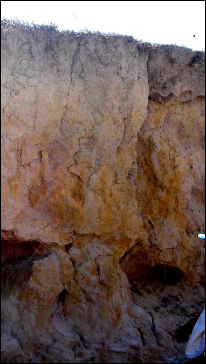
\includegraphics[keepaspectratio]{capitulos/../img/latossolo_amarelo.png}}

}

\caption{\label{fig-latossolo}Latossolo Amarelo --- solo profundo e bem
drenado, típico de planaltos tropicais.}

\end{figure}%

\end{minipage}%
%
\begin{minipage}{0.50\linewidth}

\begin{figure}[H]

\centering{

\pandocbounded{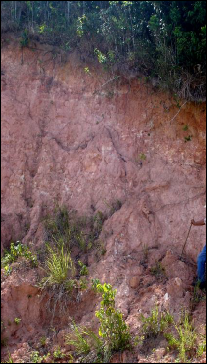
\includegraphics[keepaspectratio]{capitulos/../img/argissolo.png}}

}

\caption{\label{fig-argissolo}Argissolo Vermelho-Amarelo --- gradiente
textural com risco de deslizamento em encostas.}

\end{figure}%

\end{minipage}%

\end{figure}%

O Latossolo (Figura~\ref{fig-latossolo}) é o solo mais representativo
dos planaltos tropicais brasileiros, ocupando cerca de 39\% do
território nacional. Trata-se de um solo profundo (frequentemente
\textgreater{} 5 m), homogêneo, bem drenado e com alta agregação
conferida pelos óxidos de ferro e alumínio. Apesar de sua estabilidade
estrutural, quando desprovido de cobertura vegetal, o Latossolo é
altamente erodível pela exposição direta ao impacto das gotas de chuva,
que desagregam os microagregados superficiais. Em projetos de
bioengenharia, a prioridade é a proteção da superfície (cobertura
vegetal, biomantas, palhada) e a reconstrução da camada orgânica.

O Argissolo (Figura~\ref{fig-argissolo}) apresenta um gradiente textural
acentuado entre os horizontes A e B, com aumento expressivo no teor de
argila em profundidade. Esse gradiente cria uma descontinuidade
hidráulica que pode gerar lençol suspenso em períodos chuvosos, condição
que favorece deslizamentos translacionais. A interface entre os
horizontes A e B concentra a maior parte das rupturas, e o projeto de
bioengenharia deve priorizar a drenagem subsuperficial e a ancoragem
radicular profunda.

A Tabela~\ref{tbl-classes} sintetiza as seis principais classes de solos
tropicais e suas implicações para projetos de bioengenharia, servindo
como referência rápida para a seleção de técnicas adequadas a cada
situação de campo.

\begin{longtable}[]{@{}
  >{\raggedright\arraybackslash}p{(\linewidth - 6\tabcolsep) * \real{0.2208}}
  >{\raggedright\arraybackslash}p{(\linewidth - 6\tabcolsep) * \real{0.2208}}
  >{\raggedright\arraybackslash}p{(\linewidth - 6\tabcolsep) * \real{0.1558}}
  >{\raggedright\arraybackslash}p{(\linewidth - 6\tabcolsep) * \real{0.4026}}@{}}
\caption{Principais classes de solos tropicais e sua relevância para
projetos de bioengenharia.}\label{tbl-classes}\tabularnewline
\toprule\noalign{}
\begin{minipage}[b]{\linewidth}\raggedright
Classe (SiBCS)
\end{minipage} & \begin{minipage}[b]{\linewidth}\raggedright
WRB equivalente
\end{minipage} & \begin{minipage}[b]{\linewidth}\raggedright
Ocorrência
\end{minipage} & \begin{minipage}[b]{\linewidth}\raggedright
Relevância para bioengenharia
\end{minipage} \\
\midrule\noalign{}
\endfirsthead
\toprule\noalign{}
\begin{minipage}[b]{\linewidth}\raggedright
Classe (SiBCS)
\end{minipage} & \begin{minipage}[b]{\linewidth}\raggedright
WRB equivalente
\end{minipage} & \begin{minipage}[b]{\linewidth}\raggedright
Ocorrência
\end{minipage} & \begin{minipage}[b]{\linewidth}\raggedright
Relevância para bioengenharia
\end{minipage} \\
\midrule\noalign{}
\endhead
\bottomrule\noalign{}
\endlastfoot
Latossolo & Ferralsol & Planaltos bem drenados & Estáveis quando
cobertos, mas altamente erodíveis quando expostos; proteção superficial
prioritária \\
Argissolo & Acrisol/Lixisol & Encostas e tabuleiros & Gradiente textural
favorece deslizamentos; drenagem subsuperficial essencial \\
Plintossolo & Plinthosol & Áreas de flutuação do lençol & Endurecimento
irreversível ao secar (petroplintita); limita o enraizamento profundo \\
Neossolo Litólico & Leptosol & Encostas íngremes & Rasos (\textless{} 50
cm); alta susceptibilidade à erosão e deslizamento \\
Cambissolo & Cambisol & Relevos ondulados & Jovens e heterogêneos;
propriedades variáveis exigem investigação local \\
Gleissolo & Gleysol & Várzeas e planícies & Hidromórficos, saturados e
compressíveis; exigem espécies tolerantes a alagamento \\
\end{longtable}

\begin{figure}

\centering{

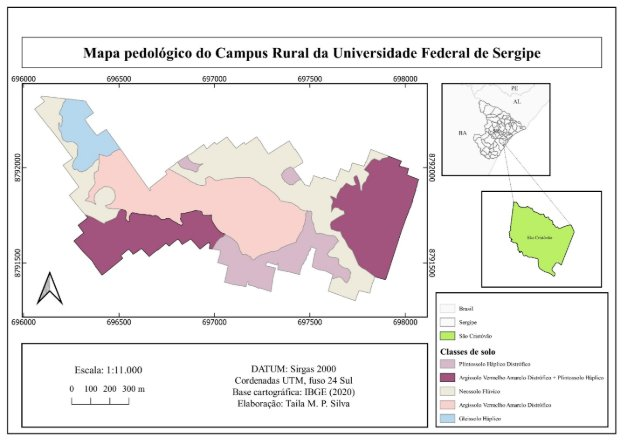
\includegraphics[width=0.8\linewidth,height=\textheight,keepaspectratio]{capitulos/../img/mapa_pedologico.jpg}

}

\caption{\label{fig-mapa-pedologico}Mapa pedológico --- distribuição
espacial das classes de solo em uma área de projeto, ferramenta
essencial para o planejamento de intervenções de bioengenharia
diferenciadas por tipo de solo.}

\end{figure}%

\chapter{Conceito de Intemperismo}\label{conceito-de-intemperismo}

\# Intemperismo e Transformação do Solo \{\#sec-intemperismo\}

O intemperismo é o conjunto de processos físicos, químicos e biológicos
que transformam rochas consolidadas em materiais inconsolidados
(saprolito e solo). Para quem trabalha com bioengenharia, compreender o
intemperismo é essencial por uma razão simples: ele é o processo que
``fabrica'' o substrato sobre o qual todas as intervenções são
projetadas. A profundidade do manto de alteração, a mineralogia das
argilas formadas e a estrutura do solo resultante são consequências
diretas da intensidade e do tipo de intemperismo atuante.

Em regiões tropicais, o intemperismo é mais intenso e profundo do que em
qualquer outra zona climática do planeta. A combinação de temperaturas
médias elevadas (\textgreater{} 20 °C), precipitação abundante
(\textgreater{} 1.200 mm/ano) e intensa atividade biológica acelera as
reações de decomposição mineral, resultando em mantos de alteração que
podem alcançar dezenas de metros de espessura. A
Figura~\ref{fig-agentes} sintetiza os agentes que atuam simultaneamente
nesse processo de transformação.

\section{Intemperismo Físico}\label{intemperismo-fuxedsico}

\begin{figure}

\centering{

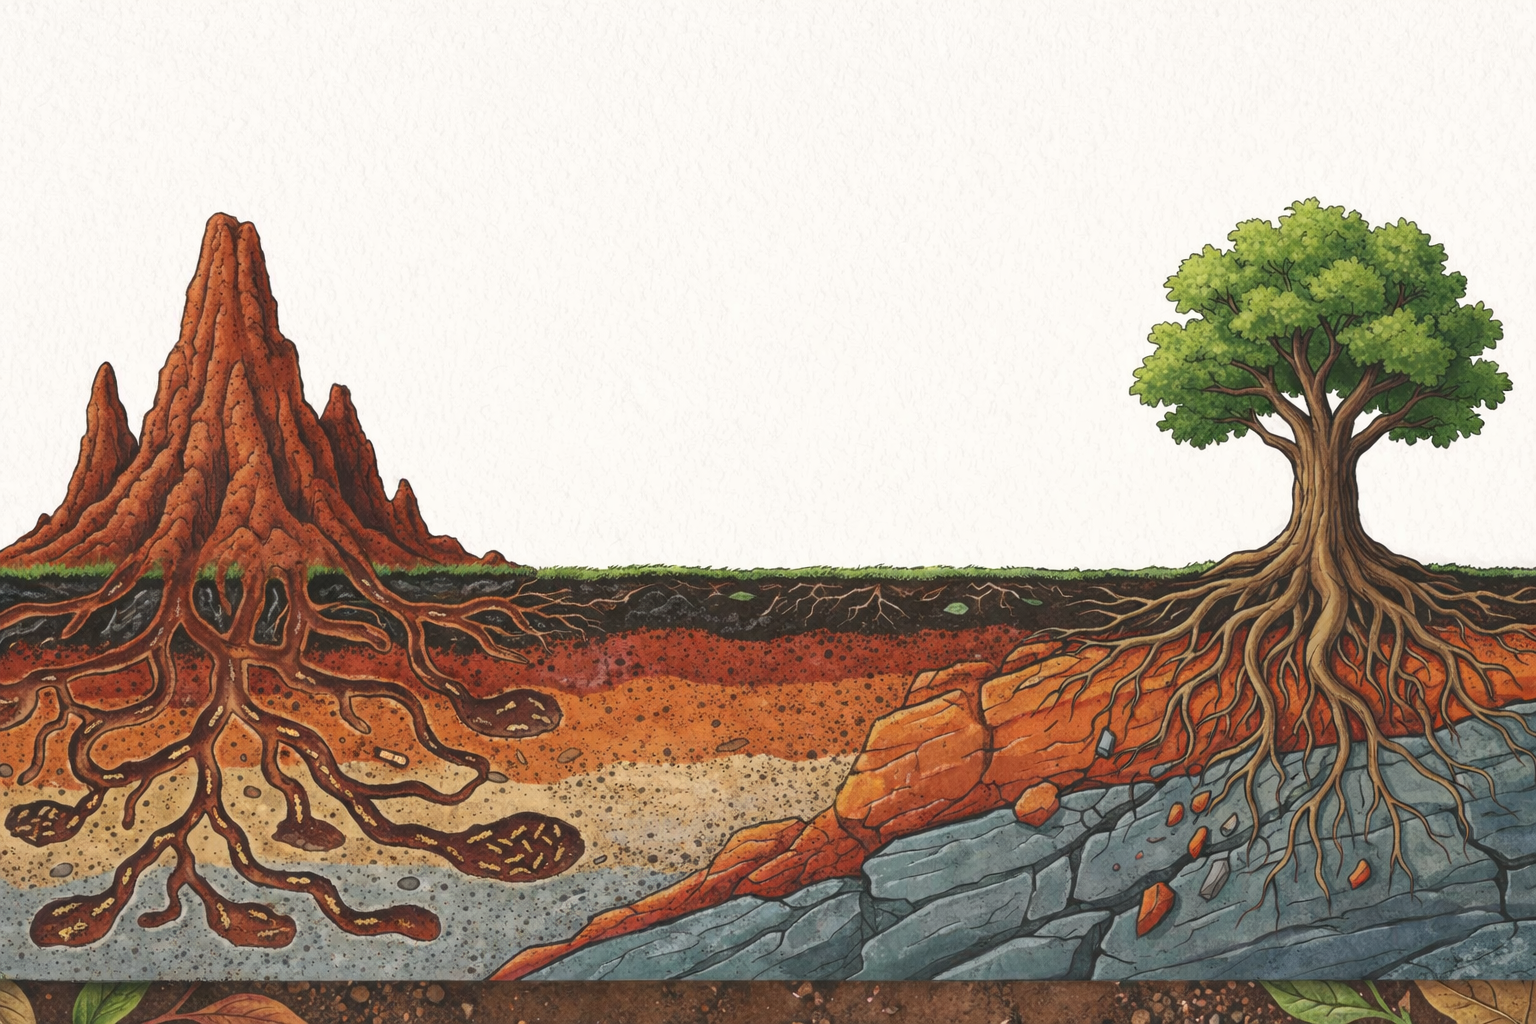
\includegraphics[width=0.8\linewidth,height=\textheight,keepaspectratio]{capitulos/../img/agentes_ativos.png}

}

\caption{\label{fig-agentes}Agentes do intemperismo atuando sobre a
rocha: processos físicos, químicos e biológicos que transformam a rocha
em solo.}

\end{figure}%

O intemperismo físico fragmenta mecanicamente a rocha sem alterar sua
composição mineralógica. Trata-se da ``quebra'' da rocha em pedaços cada
vez menores, aumentando a superfície específica exposta e, com isso,
acelerando o ataque químico subsequente. É importante compreender que o
intemperismo físico não atua sozinho; ele prepara o terreno para o
intemperismo químico, que será o agente dominante nos trópicos. Os
principais mecanismos em regiões tropicais são descritos a seguir.

\subsection{Alívio de Pressão}\label{aluxedvio-de-pressuxe3o}

Quando rochas formadas em grande profundidade (sob pressão de
quilômetros de material sobrejacente) são gradualmente expostas à
superfície pela remoção erosiva das camadas superiores, a descompressão
gera fraturas subparalelas à topografia, fenômeno conhecido como
\emph{sheet joints} ou \emph{sheeting}. Esse processo é visível na
Figura~\ref{fig-alivio}.

\begin{figure}

\centering{

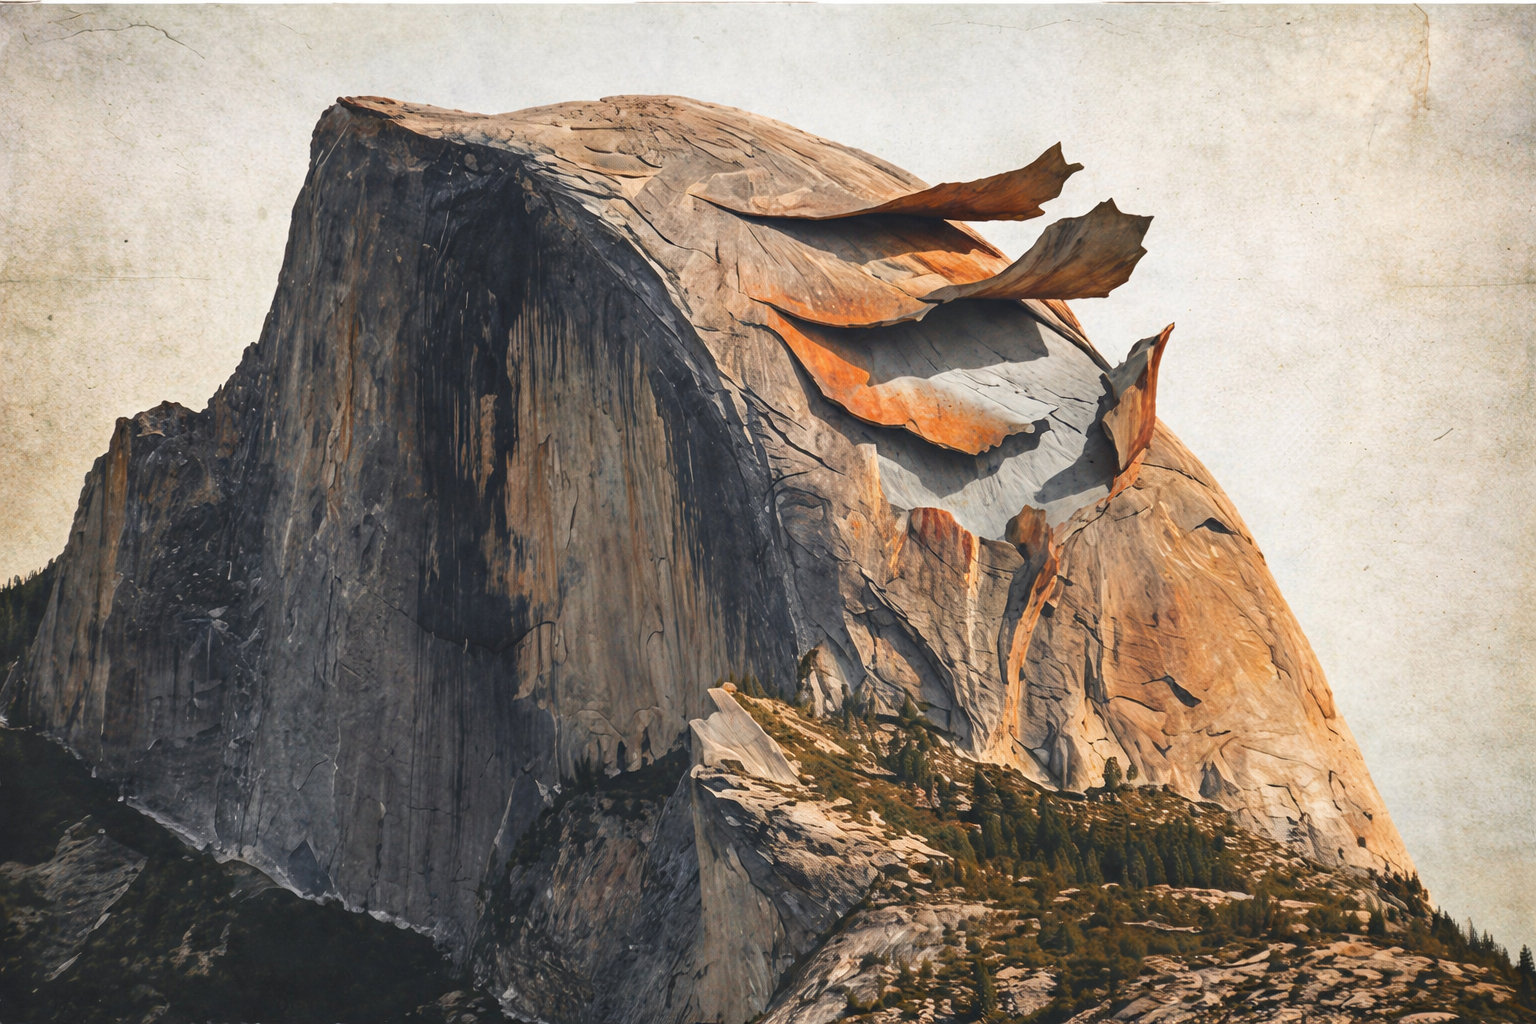
\includegraphics[width=0.7\linewidth,height=\textheight,keepaspectratio]{capitulos/../img/alivio_pressao.png}

}

\caption{\label{fig-alivio}Fraturas geradas por alívio de pressão em
rochas graníticas --- a descompressão gera sistemas de fraturas
subparalelas à superfície.}

\end{figure}%

Esse mecanismo é particularmente importante em maciços graníticos e
gnáissicos nos inselbergs do Nordeste brasileiro, onde as fraturas
geradas pelo alívio de pressão criam caminhos preferenciais para a
infiltração da água, acelerando o intemperismo químico nos planos de
descontinuidade. Em termos práticos, encostas rochosas com
\emph{sheeting} bem desenvolvido são mais suscetíveis a desprendimentos
de lajes e blocos, o que deve ser considerado no projeto de
intervenções.

\subsection{Termoclastia}\label{termoclastia}

A variação diurna de temperatura causa expansão e contração diferencial
dos minerais que compõem a rocha. Como cada mineral tem um coeficiente
de dilatação térmica diferente, os ciclos de aquecimento e resfriamento
geram tensões internas heterogêneas que, com o tempo, produzem
microfissuras e fraturam progressivamente a rocha. A
Figura~\ref{fig-termoclastia} ilustra esse processo.

\begin{figure}

\centering{

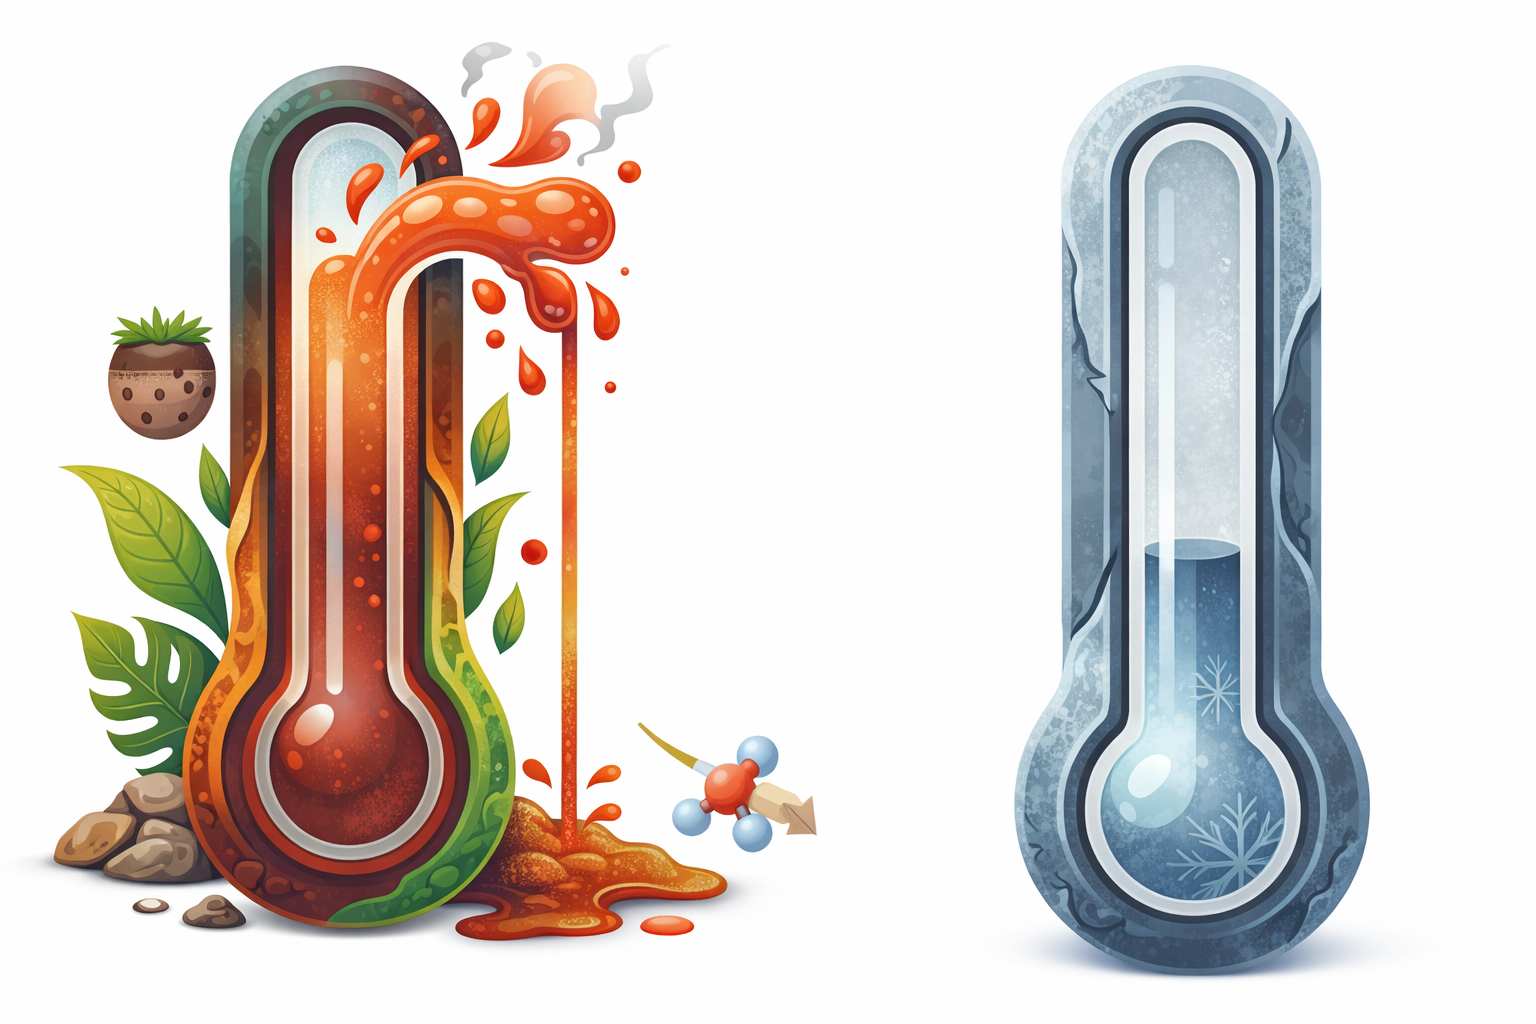
\includegraphics[width=0.65\linewidth,height=\textheight,keepaspectratio]{capitulos/../img/termoclastia.png}

}

\caption{\label{fig-termoclastia}Variação de temperatura diurna em
superfícies rochosas --- a amplitude térmica gera tensões de expansão e
contração nos minerais.}

\end{figure}%

Em regiões semiáridas tropicais (como a Caatinga brasileira), a
amplitude térmica superficial pode alcançar 60 °C (rocha exposta ao sol
a 70 °C versus ar noturno a 10 °C), gerando tensões suficientes para
fraturar até rochas muito competentes. A termoclastia é um dos fatores
que explicam a produção de cascalho e areia grossa nos pedimentos
semiáridos, materiais que podem ser aproveitados como agregados em
estruturas de bioengenharia.

\subsection{Crescimento de Cristais}\label{crescimento-de-cristais}

Em ambientes semiáridos, a evaporação de soluções salinas nos poros e
fraturas da rocha gera cristais de sais (cloretos, sulfatos, carbonatos)
que exercem pressão de cristalização de até 300 MPa sobre as paredes dos
poros, fragmentando progressivamente o substrato. Esse processo, chamado
haloclastia, é responsável pela degradação acelerada de rochas em
ambientes costeiros e em regiões com solos salinos, sendo especialmente
relevante em obras de bioengenharia no Semiárido nordestino.

\subsection{Ação Biológica
Mecânica}\label{auxe7uxe3o-bioluxf3gica-mecuxe2nica}

As raízes de árvores e arbustos penetram fraturas preexistentes e
exercem pressão mecânica de expansão à medida que crescem em diâmetro.
Esse processo, chamado \emph{root wedging}, é capaz de fragmentar blocos
de rocha ao longo de décadas. Liquens e fungos contribuem para a
fragmentação superficial combinando ação mecânica (hifas que penetram
microfissuras) e ação química (exsudação de ácidos orgânicos). Para a
bioengenharia, isso tem uma implicação paradoxal: embora o enraizamento
seja desejável para estabilizar taludes de solo, raízes penetrando
fraturas de rocha podem desestabilizar encostas rochosas.

\section{Intemperismo Químico}\label{intemperismo-quuxedmico}

O intemperismo químico é o processo dominante nos trópicos úmidos,
responsável por transformar minerais primários (formados a altas
temperaturas e pressões durante a consolidação da rocha) em minerais
secundários (argilas e óxidos estáveis nas condições de superfície). A
água é o agente principal dessas transformações, e sua abundância nos
trópicos explica por que os solos tropicais são os mais profundamente
intemperizados do planeta.

\subsection{Papel da Água}\label{papel-da-uxe1gua}

A molécula de água desempenha três funções simultâneas e indissociáveis
no intemperismo químico. Atua como solvente (dissolvendo íons e
moléculas dos minerais por sua elevada constante dielétrica), como
reagente (participando diretamente das reações de hidrólise, que são as
mais importantes nos trópicos) e como meio de transporte (removendo
produtos solúveis por lixiviação e redistribuindo materiais ao longo do
perfil).

A taxa de intemperismo químico aumenta exponencialmente com a
temperatura, seguindo a Lei de Arrhenius:

\[
k = A \cdot e^{-E_a / RT}
\]

onde \(k\) é a constante de velocidade da reação, \(A\) é o fator de
frequência (frequência com que as moléculas colidem com orientação
favorável), \(E_a\) é a energia de ativação (barreira energética que
deve ser superada para que a reação ocorra), \(R\) é a constante
universal dos gases (8,314 J mol⁻¹ K⁻¹) e \(T\) é a temperatura absoluta
(em kelvin). Em termos práticos, cada aumento de 10 °C na temperatura
duplica aproximadamente a velocidade das reações de intemperismo, o que
explica por que solos tropicais atingem graus de intemperismo que solos
temperados levariam milhões de anos adicionais para alcançar.

\subsection{Principais Reações}\label{principais-reauxe7uxf5es}

A hidrólise constitui a reação mais importante nos trópicos, pois é o
mecanismo pelo qual os silicatos (minerais dominantes nas rochas da
crosta) são decompostos pela ação de íons H⁺ da água. O exemplo clássico
é a hidrólise do feldspato potássico (ortoclásio, um dos minerais mais
comuns em granitos) para caulinita (a argila dominante nos solos
tropicais):

\[
2 \text{KAlSi}_3\text{O}_8 + 2\text{H}^+ + 9\text{H}_2\text{O} \rightarrow \text{Al}_2\text{Si}_2\text{O}_5(\text{OH})_4 + 4\text{H}_4\text{SiO}_4 + 2\text{K}^+
\]

Note que a reação consome dois moles de feldspato e produz caulinita
(que permanece no solo) e sílica dissolvida e potássio em solução (que
são exportados pela drenagem). Essa exportação contínua de sílica e
bases é responsável pelo empobrecimento químico progressivo dos solos
tropicais.

A oxidação promove a conversão de ferro ferroso (Fe²⁺, solúvel) em ferro
férrico (Fe³⁺, insolúvel), formando os óxidos de ferro responsáveis
pelas cores vermelhas e amarelas características dos solos tropicais:

\[
4\text{Fe}^{2+} + 3\text{O}_2 + 6\text{H}_2\text{O} \rightarrow 4\text{FeOOH} + 8\text{H}^+
\]

O produto dessa reação (goethita, FeOOH) é um dos minerais mais estáveis
nas condições tropicais e desempenha papel fundamental na microagregação
dos solos lateríticos, conferindo-lhes estabilidade estrutural mesmo com
altos teores de argila. Esse é um aspecto positivo para a bioengenharia,
pois a microagregação facilita a infiltração e a penetração radicular.

A dissolução corresponde à remoção completa de íons solúveis (Ca²⁺,
Mg²⁺, K⁺, Na⁺) pela lixiviação, concentrando residualmente os óxidos de
ferro e alumínio mais insolúveis. É esse processo de empobrecimento
seletivo que transforma, ao longo de milhões de anos, uma rocha rica em
diversos minerais em um solo dominado por caulinita, goethita e
gibbsita.

\subsection{Série de Goldich}\label{suxe9rie-de-goldich}

A série de estabilidade de Goldich (inversa da série de cristalização de
Bowen) ordena os minerais segundo sua resistência ao intemperismo.
Minerais formados em altas temperaturas e pressões (primeiros a
cristalizar no magma) são os menos estáveis nas condições de superfície
e, portanto, os primeiros a serem destruídos pelo intemperismo.

\begin{longtable}[]{@{}ll@{}}
\caption{Série de estabilidade de Goldich, onde minerais formados em
altas temperaturas (esquerda) são os primeiros a
intemperizar.}\label{tbl-goldich}\tabularnewline
\toprule\noalign{}
Mais susceptível → & → Menos susceptível \\
\midrule\noalign{}
\endfirsthead
\toprule\noalign{}
Mais susceptível → & → Menos susceptível \\
\midrule\noalign{}
\endhead
\bottomrule\noalign{}
\endlastfoot
Olivina & Quartzo \\
Piroxênio & Muscovita \\
Anfibólio & Feldspato potássico \\
Biotita & --- \\
\end{longtable}

Para a bioengenharia, a série de Goldich tem uma implicação prática
imediata. Solos derivados de rochas ricas em olivina e piroxênio (como
basaltos) intemperizam rapidamente e produzem solos argilosos profundos
(Latossolos), enquanto solos derivados de rochas quartzosas (como
arenitos) geram solos arenosos rasos com baixa coesão e alta
erodibilidade. A identificação da rocha-mãe permite, portanto, antecipar
as propriedades do solo e selecionar as técnicas de bioengenharia mais
adequadas.

\section{Índice de Intemperismo Químico
(CIA)}\label{uxedndice-de-intemperismo-quuxedmico-cia}

Para quantificar objetivamente o grau de intemperismo de um solo ou
saprolito, utiliza-se o Chemical Index of Alteration (CIA), proposto por
Nesbitt e Young (1982):

\[
\text{CIA} = \frac{\text{Al}_2\text{O}_3}{\text{Al}_2\text{O}_3 + \text{CaO}^* + \text{Na}_2\text{O} + \text{K}_2\text{O}} \times 100
\]

O CIA mede a proporção de alumínio (que permanece no solo como argilas e
hidróxidos) em relação à soma de alumínio e bases (cálcio, sódio e
potássio, que são progressivamente removidos pela lixiviação). Quanto
mais alto o CIA, mais intenso foi o intemperismo. A Tabela~\ref{tbl-cia}
apresenta a interpretação dos valores.

\begin{longtable}[]{@{}lll@{}}
\caption{Interpretação do CIA para diferentes graus de
intemperismo.}\label{tbl-cia}\tabularnewline
\toprule\noalign{}
CIA & Grau de intemperismo & Exemplo \\
\midrule\noalign{}
\endfirsthead
\toprule\noalign{}
CIA & Grau de intemperismo & Exemplo \\
\midrule\noalign{}
\endhead
\bottomrule\noalign{}
\endlastfoot
50 & Rocha fresca & Granito inalterado \\
60--70 & Moderado & Solos de zona temperada \\
75--85 & Avançado & Argissolos tropicais \\
85--100 & Extremo & Latossolos, bauxitas \\
\end{longtable}

\section{Minerais Diagnósticos dos Solos
Tropicais}\label{minerais-diagnuxf3sticos-dos-solos-tropicais}

Os produtos finais do intemperismo nos trópicos são um conjunto restrito
de minerais muito estáveis que dominam a mineralogia dos solos.
Conhecê-los é fundamental para a bioengenharia, pois cada mineral
confere propriedades geotécnicas e químicas distintas ao solo.

\subsection{Caulinita}\label{caulinita}

A caulinita é uma argila do tipo 1:1 (uma lâmina tetraédrica de sílica
ligada a uma lâmina octaédrica de alumina), com espaçamento basal de 7,2
Å. Trata-se do argilomineral mais abundante nos solos tropicais bem
drenados, sendo o produto direto da hidrólise dos feldspatos conforme
discutido acima. A Figura~\ref{fig-caulinita} mostra a aparência
característica desse mineral ao microscópio.

\begin{figure}

\centering{

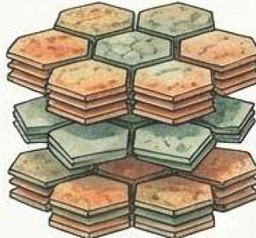
\includegraphics[width=0.6\linewidth,height=\textheight,keepaspectratio]{capitulos/../img/caulinita.jpg}

}

\caption{\label{fig-caulinita}Caulinita --- argilomineral 1:1 dominante
nos solos tropicais bem drenados, com baixa CTC e expansibilidade.}

\end{figure}%

Para a bioengenharia, as propriedades da caulinita têm implicações
diretas. Sua baixa capacidade de troca catiônica (CTC ≈ 3--15 cmolc/kg,
contra 80--150 cmolc/kg em argilas montmoriloníticas) significa que
solos cauliníticos retêm poucos nutrientes, exigindo adição de matéria
orgânica para sustentar o crescimento vegetal. Sua baixa expansibilidade
(não incha nem contrai com variações de umidade, diferentemente das
argilas 2:1) confere estabilidade volumétrica ao solo, o que é vantajoso
para estruturas construídas sobre ele. Sua coesão moderada explica a
estabilidade aparente dos solos tropicais secos, mas a perda rápida de
resistência quando saturados.

\subsection{Goethita (FeOOH)}\label{goethita-feooh}

A goethita é o óxido de ferro responsável pela cor amarela dos solos
tropicais. Predomina em ambientes mais úmidos e com menor variação
sazonal de umidade (como topos de morro sombreados ou solos de encostas
voltadas para o sul no hemisfério sul). A goethita cristaliza com maior
teor de água em sua estrutura e reflete a luz na faixa do amarelo-ocre.
Em termos geotécnicos, a presença dominante de goethita em relação à
hematita indica solos com regime hídrico mais úmido, o que deve ser
considerado no dimensionamento da drenagem em projetos de bioengenharia.

\subsection{Hematita (Fe₂O₃)}\label{hematita-feux2082oux2083}

A hematita é o óxido de ferro que confere a cor vermelha intensa aos
solos tropicais, sendo o resultado da desidratação da goethita em
condições de boa drenagem e estação seca definida. A
Figura~\ref{fig-hematita} ilustra a coloração característica desse
mineral.

\begin{figure}

\centering{

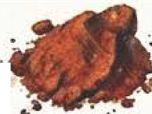
\includegraphics[width=0.6\linewidth,height=\textheight,keepaspectratio]{capitulos/../img/hematita.png}

}

\caption{\label{fig-hematita}Hematita --- óxido de ferro que confere a
coloração vermelha característica dos solos tropicais bem drenados.}

\end{figure}%

A hematita possui papel fundamental na microagregação dos solos
tropicais (Latossolos). Ela atua como agente cimentante entre partículas
de caulinita, formando microagregados esféricos de 0,1--1,0 mm de
diâmetro que conferem ao solo uma estrutura granular extremamente
estável e, paradoxalmente, fazem com que solos com 60--80\% de argila se
comportem hidraulicamente como areias (alta permeabilidade, baixa
plasticidade). Essa microagregação é benéfica para a bioengenharia por
facilitar a infiltração e o enraizamento, mas é destruída por
compactação ou erosão superficial intensa.

\subsection{Gibbsita (Al(OH)₃)}\label{gibbsita-alohux2083}

A gibbsita é um hidróxido de alumínio indicador de intemperismo extremo
(ferraltização). Sua presença abundante indica que o solo perdeu
praticamente toda a sílica por lixiviação, restando apenas alumínio e
ferro como componentes minerais. É o mineral diagnóstico dos Latossolos
mais intemperizados e das bauxitas (minério de alumínio). Em termos de
bioengenharia, solos com alto teor de gibbsita são extremamente pobres
em nutrientes (CTC da gibbsita ≈ 0) e exigem adição massiva de matéria
orgânica para qualquer estratégia de revegetação.

\section{Implicações para a
Bioengenharia}\label{implicauxe7uxf5es-para-a-bioengenharia}

O grau de intemperismo determina diretamente as propriedades geotécnicas
do solo e, consequentemente, as decisões de projeto de bioengenharia. A
compreensão da mineralogia e da evolução geoquímica do perfil permite
antecipar comportamentos e selecionar técnicas com maior probabilidade
de sucesso.

\begin{tcolorbox}[enhanced jigsaw, leftrule=.75mm, colframe=quarto-callout-warning-color-frame, colback=white, bottomrule=.15mm, opacityback=0, colbacktitle=quarto-callout-warning-color!10!white, breakable, bottomtitle=1mm, opacitybacktitle=0.6, title=\textcolor{quarto-callout-warning-color}{\faExclamationTriangle}\hspace{0.5em}{Atenção}, titlerule=0mm, toprule=.15mm, toptitle=1mm, rightrule=.15mm, left=2mm, arc=.35mm, coltitle=black]

Solos extremamente intemperizados (CIA \textgreater{} 85) apresentam um
conjunto de propriedades que exige abordagens específicas de
bioengenharia. A baixa CTC (dominada por caulinita e gibbsita) demanda
reposição contínua de matéria orgânica para viabilizar o crescimento
vegetal. A coesão aparente (conferida por cimentação por óxidos e sucção
matricial) implica estabilidade temporária que é rapidamente perdida
quando o solo satura, tornando essencial o gerenciamento da drenagem. A
microagregação por óxidos de ferro gera comportamento pseudo-arenoso
(alta permeabilidade em solo argiloso), o que pode parecer contraditório
mas facilita tanto o enraizamento quanto a drenagem interna.

\end{tcolorbox}

Essas propriedades influenciam diretamente a seleção de técnicas. A
baixa CTC demanda técnicas que agreguem matéria orgânica (mulch,
biomantas, hidrossemeadura com compostos orgânicos), enquanto a coesão
aparente torna essencial a drenagem superficial e subsuperficial para
evitar saturação e colapso. Por outro lado, a microagregação facilita a
penetração radicular, favorecendo técnicas vegetativas que se beneficiam
da estrutura granular do solo. Em resumo, cada decisão de projeto de
bioengenharia em solos tropicais deve ser fundamentada no conhecimento
do grau de intemperismo e da mineralogia dominante do perfil.

\chapter{Conceito e Magnitude}\label{conceito-e-magnitude}

\# Erosão do Solo: Tipos e Processos \{\#sec-erosao\}

A erosão hídrica é o processo de desprendimento, transporte e deposição
de partículas de solo pela ação da água. Embora a erosão seja um
fenômeno natural que ocorre em todas as paisagens (sendo, de fato, o
agente modelador do relevo terrestre ao longo do tempo geológico), as
atividades humanas (desmatamento, agricultura intensiva, urbanização)
aceleraram esse processo em taxas que superam em 10 a 100 vezes a erosão
natural. Em escala global, estima-se que 75 bilhões de toneladas de solo
sejam erodidas anualmente, com custo econômico superior a US\$ 400
bilhões/ano (Morgan, 2005), considerando-se perdas de produtividade
agrícola, assoreamento de reservatórios, degradação da qualidade da água
e destruição de infraestrutura.

Para quem atua em bioengenharia de solos, compreender os mecanismos
erosivos é o ponto de partida obrigatório, pois cada tipo de erosão
demanda técnicas de controle específicas. Um tratamento projetado para
erosão laminar será ineficaz contra uma voçoroca ativa, e vice-versa.

Em regiões tropicais, a erosividade da chuva (fator R da RUSLE) é
tipicamente 3 a 5 vezes maior do que em zonas temperadas, devido à maior
frequência de chuvas convectivas intensas (com gotas de grande diâmetro
e alta energia cinética), tornando a erosão um dos processos
geomorfológicos mais ativos e um dos maiores desafios ambientais do
Brasil.

\section{RUSLE (Equação Universal de Perda de
Solo)}\label{rusle-equauxe7uxe3o-universal-de-perda-de-solo}

O modelo RUSLE (\emph{Revised Universal Soil Loss Equation}) (Renard et
al., 1997) é a ferramenta mais amplamente utilizada para estimar a perda
de solo por erosão laminar e em sulcos. Apesar de suas limitações (não
modela erosão em ravinas nem deposição), a RUSLE é fundamental para o
planejamento de intervenções de bioengenharia, pois permite quantificar
a perda de solo atual e simular a eficácia de diferentes práticas
conservacionistas antes de sua implantação.

\[
A = R \cdot K \cdot L \cdot S \cdot C \cdot P
\]

A Tabela~\ref{tbl-rusle} descreve cada fator da equação. É importante
notar que o resultado (\(A\)) expressa a média anual de perda de solo em
toneladas por hectare por ano, e que a equação assume condições de
estado estacionário para uma encosta retilínea com comprimento e
declividade uniformes.

\begin{longtable}[]{@{}
  >{\raggedright\arraybackslash}p{(\linewidth - 6\tabcolsep) * \real{0.1591}}
  >{\raggedright\arraybackslash}p{(\linewidth - 6\tabcolsep) * \real{0.2727}}
  >{\raggedright\arraybackslash}p{(\linewidth - 6\tabcolsep) * \real{0.2045}}
  >{\raggedright\arraybackslash}p{(\linewidth - 6\tabcolsep) * \real{0.3636}}@{}}
\caption{Fatores da RUSLE e suas
unidades.}\label{tbl-rusle}\tabularnewline
\toprule\noalign{}
\begin{minipage}[b]{\linewidth}\raggedright
Fator
\end{minipage} & \begin{minipage}[b]{\linewidth}\raggedright
Significado
\end{minipage} & \begin{minipage}[b]{\linewidth}\raggedright
Unidade
\end{minipage} & \begin{minipage}[b]{\linewidth}\raggedright
O que controla
\end{minipage} \\
\midrule\noalign{}
\endfirsthead
\toprule\noalign{}
\begin{minipage}[b]{\linewidth}\raggedright
Fator
\end{minipage} & \begin{minipage}[b]{\linewidth}\raggedright
Significado
\end{minipage} & \begin{minipage}[b]{\linewidth}\raggedright
Unidade
\end{minipage} & \begin{minipage}[b]{\linewidth}\raggedright
O que controla
\end{minipage} \\
\midrule\noalign{}
\endhead
\bottomrule\noalign{}
\endlastfoot
\(A\) & Perda de solo & t ha⁻¹ ano⁻¹ & Resultado do modelo \\
\(R\) & Erosividade da chuva & MJ mm ha⁻¹ h⁻¹ ano⁻¹ & Energia e
intensidade das chuvas \\
\(K\) & Erodibilidade do solo & t h MJ⁻¹ mm⁻¹ & Susceptibilidade
intrínseca do solo \\
\(L\) & Comprimento da rampa & adimensional & Distância percorrida pelo
escoamento \\
\(S\) & Declividade & adimensional & Inclinação da encosta \\
\(C\) & Uso e manejo do solo & adimensional & Cobertura e práticas
culturais \\
\(P\) & Práticas conservacionistas & adimensional & Intervenções de
controle da erosão \\
\end{longtable}

\begin{tcolorbox}[enhanced jigsaw, leftrule=.75mm, colframe=quarto-callout-tip-color-frame, colback=white, bottomrule=.15mm, opacityback=0, colbacktitle=quarto-callout-tip-color!10!white, breakable, bottomtitle=1mm, opacitybacktitle=0.6, title=\textcolor{quarto-callout-tip-color}{\faLightbulb}\hspace{0.5em}{Parâmetro-chave para bioengenharia}, titlerule=0mm, toprule=.15mm, toptitle=1mm, rightrule=.15mm, left=2mm, arc=.35mm, coltitle=black]

Os fatores \(C\) e \(P\) são os diretamente manipuláveis pela
bioengenharia. Uma cobertura de gramíneas pode reduzir \(C\) de 1,0
(solo nu) para 0,01, representando uma redução de 99\% na erosão. Da
mesma forma, paliçadas ou cordões vegetativos reduzem efetivamente o
fator \(L\) (comprimento da rampa), enquanto terraços alteram o fator
\(S\) (declividade). A combinação dessas intervenções pode reduzir a
perda de solo de centenas de toneladas por hectare/ano para valores
abaixo da tolerância.

\end{tcolorbox}

\section{Método SCS-CN para Estimativa de
Escoamento}\label{muxe9todo-scs-cn-para-estimativa-de-escoamento}

Além da RUSLE, que estima a perda de solo por erosão laminar, o
projetista de bioengenharia necessita estimar o volume e o pico de
escoamento superficial gerado por eventos de chuva, informação essencial
para dimensionar paliçadas (ver \textbf{?@sec-palicadas}), bacias de
captação (ver \textbf{?@sec-bacias-captacao}) e canaletas verdes (ver
\textbf{?@sec-canaleta-verde}). O método SCS-CN (\emph{Soil Conservation
Service --- Curve Number}), desenvolvido pelo USDA, é a ferramenta mais
amplamente utilizada para essa finalidade.

O escoamento superficial direto (\(Q\), em mm) gerado por uma
precipitação total (\(P\), em mm) é estimado por

\[
Q = \frac{(P - 0{,}2S)^2}{P + 0{,}8S}
\]

válida para \(P > 0{,}2S\) (caso contrário, \(Q = 0\)), onde \(S\) é a
retenção potencial máxima do solo (mm), calculada a partir do
\emph{Curve Number} (\(CN\)) pela relação

\[
S = \frac{25400}{CN} - 254
\]

O \(CN\) é um parâmetro adimensional (0--100) que integra os efeitos do
tipo hidrológico do solo, da cobertura vegetal e da condição de umidade
antecedente. A Tabela~\ref{tbl-cn} apresenta valores de \(CN\) para
condições típicas em projetos de bioengenharia no Brasil tropical.

\begin{longtable}[]{@{}
  >{\raggedright\arraybackslash}p{(\linewidth - 8\tabcolsep) * \real{0.3514}}
  >{\raggedright\arraybackslash}p{(\linewidth - 8\tabcolsep) * \real{0.1622}}
  >{\raggedright\arraybackslash}p{(\linewidth - 8\tabcolsep) * \real{0.1622}}
  >{\raggedright\arraybackslash}p{(\linewidth - 8\tabcolsep) * \real{0.1622}}
  >{\raggedright\arraybackslash}p{(\linewidth - 8\tabcolsep) * \real{0.1622}}@{}}
\caption{Valores de CN para condições típicas de projetos de
bioengenharia em solos tropicais (condição de umidade antecedente
II).}\label{tbl-cn}\tabularnewline
\toprule\noalign{}
\begin{minipage}[b]{\linewidth}\raggedright
Uso do solo / cobertura
\end{minipage} & \begin{minipage}[b]{\linewidth}\raggedright
Solo tipo A
\end{minipage} & \begin{minipage}[b]{\linewidth}\raggedright
Solo tipo B
\end{minipage} & \begin{minipage}[b]{\linewidth}\raggedright
Solo tipo C
\end{minipage} & \begin{minipage}[b]{\linewidth}\raggedright
Solo tipo D
\end{minipage} \\
\midrule\noalign{}
\endfirsthead
\toprule\noalign{}
\begin{minipage}[b]{\linewidth}\raggedright
Uso do solo / cobertura
\end{minipage} & \begin{minipage}[b]{\linewidth}\raggedright
Solo tipo A
\end{minipage} & \begin{minipage}[b]{\linewidth}\raggedright
Solo tipo B
\end{minipage} & \begin{minipage}[b]{\linewidth}\raggedright
Solo tipo C
\end{minipage} & \begin{minipage}[b]{\linewidth}\raggedright
Solo tipo D
\end{minipage} \\
\midrule\noalign{}
\endhead
\bottomrule\noalign{}
\endlastfoot
Floresta densa (Mata Atlântica) & 25 & 55 & 70 & 77 \\
Cerrado denso & 36 & 60 & 73 & 79 \\
Pastagem em boas condições & 39 & 61 & 74 & 80 \\
Pastagem degradada (solo exposto \textgreater{} 50\%) & 68 & 79 & 86 &
89 \\
Solo nu (pós-desmatamento) & 77 & 86 & 91 & 94 \\
Estrada rural não pavimentada & 72 & 82 & 87 & 89 \\
\end{longtable}

\begin{tcolorbox}[enhanced jigsaw, leftrule=.75mm, colframe=quarto-callout-tip-color-frame, colback=white, bottomrule=.15mm, opacityback=0, colbacktitle=quarto-callout-tip-color!10!white, breakable, bottomtitle=1mm, opacitybacktitle=0.6, title=\textcolor{quarto-callout-tip-color}{\faLightbulb}\hspace{0.5em}{Aplicação prática}, titlerule=0mm, toprule=.15mm, toptitle=1mm, rightrule=.15mm, left=2mm, arc=.35mm, coltitle=black]

A redução do \(CN\) é o objetivo hidrológico de qualquer intervenção de
bioengenharia. Ao converter uma pastagem degradada (\(CN = 86\), solo
tipo C) em uma encosta revegetada com espécies nativas
(\(CN \approx 73\)), a retenção potencial \(S\) aumenta de 41 mm para 94
mm, reduzindo o escoamento gerado por uma chuva de 80 mm de 35,5 mm para
11,6 mm, o que representa uma diminuição de 67\% no volume de enxurrada.
Esse cálculo justifica tecnicamente a prioridade dada à revegetação em
projetos de controle de erosão.

\end{tcolorbox}

A vazão de pico (\(Q_p\)) pode ser estimada pelo método racional
modificado do SCS, que incorpora o tempo de concentração da bacia

\[
Q_p = \frac{0{,}208 \cdot A \cdot Q}{t_p}
\]

onde \(A\) é a área da bacia contribuinte (km²), \(Q\) é o escoamento
direto (mm, calculado pela equação anterior) e \(t_p\) é o tempo de pico
(h), dado por \(t_p = 0{,}6 \cdot t_c\) (onde \(t_c\) é o tempo de
concentração estimado pela fórmula de Kirpich ou equivalente). Essa
vazão de pico é o dado de entrada para o dimensionamento hidráulico das
estruturas de dissipação, contenção e condução de enxurrada, conforme
detalhado nos capítulos subsequentes.

\section{Tipos de Erosão}\label{tipos-de-erosuxe3o}

A erosão hídrica se manifesta em diferentes formas, que representam um
contínuo de intensidade crescente. A Figura~\ref{fig-tipos-erosao}
apresenta uma comparação visual desses tipos, desde a erosão laminar
(praticamente imperceptível) até as feições lineares de grande porte.

\begin{figure}

\centering{

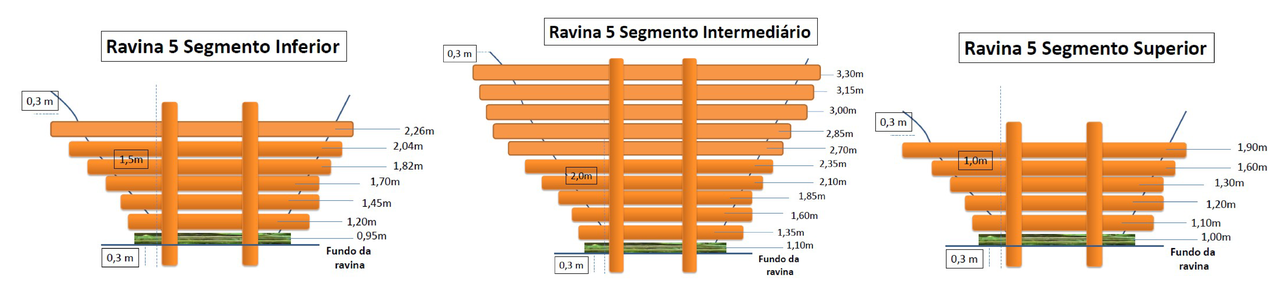
\includegraphics[width=0.9\linewidth,height=\textheight,keepaspectratio]{capitulos/../img/ravina_montagem.png}

}

\caption{\label{fig-tipos-erosao}Comparação visual dos tipos de erosão:
desde a erosão laminar até a formação de ravinas e voçorocas em solos
tropicais.}

\end{figure}%

\subsection{\texorpdfstring{Erosão Laminar (\emph{Sheet
Erosion})}{Erosão Laminar (Sheet Erosion)}}\label{erosuxe3o-laminar-sheet-erosion}

A erosão laminar consiste na remoção uniforme de uma fina camada de solo
pela ação do escoamento superficial difuso (uma lâmina d'água rasa que
escoa uniformemente sobre a superfície). É a forma mais insidiosa de
erosão por ser visualmente imperceptível; o agricultor perde solo
progressivamente sem notar, até que a exposição dos horizontes
subsuperficiais (mais claros, mais compactos) revele a gravidade da
situação. Em regiões tropicais, a erosão laminar sob chuvas intensas
pode remover 1--3 mm de solo por evento, o que equivale a 15--45 t/ha. A
proteção da superfície por cobertura vegetal viva, morta (mulch) ou
artificial (biomantas) é a estratégia primária de controle.

\subsection{\texorpdfstring{Erosão em Sulcos (\emph{Rill
Erosion})}{Erosão em Sulcos (Rill Erosion)}}\label{erosuxe3o-em-sulcos-rill-erosion}

Quando o escoamento superficial se concentra em pequenos canais
paralelos à encosta (com profundidade inferior a 30 cm), escava-se uma
rede de sulcos que concentra progressivamente o fluxo de água e
sedimentos. Os sulcos ainda podem ser desfeitos por operações agrícolas
convencionais (aração, gradagem), o que os distingue das ravinas.
Entretanto, se não corrigidos, representam o estágio inicial da formação
de feições erosivas permanentes. O controle se dá pela redução do
comprimento da rampa (implantação de cordões vegetativos, paliçadas ou
terraços que interrompem o escoamento concentrado).

\subsection{\texorpdfstring{Erosão em Ravinas (\emph{Gully
Erosion})}{Erosão em Ravinas (Gully Erosion)}}\label{erosuxe3o-em-ravinas-gully-erosion}

A ravina é um canal permanente com profundidade superior a 30 cm que não
pode ser eliminado por operações agrícolas convencionais. Representa o
estágio avançado da erosão hídrica concentrada e é o tipo de feição
erosiva que mais demanda intervenções de bioengenharia. A
Figura~\ref{fig-ravina-campo} mostra uma ravina ativa em solo tropical,
onde é possível observar as paredes verticais expostas e a ausência de
cobertura vegetal no interior do canal.

\begin{figure}

\centering{

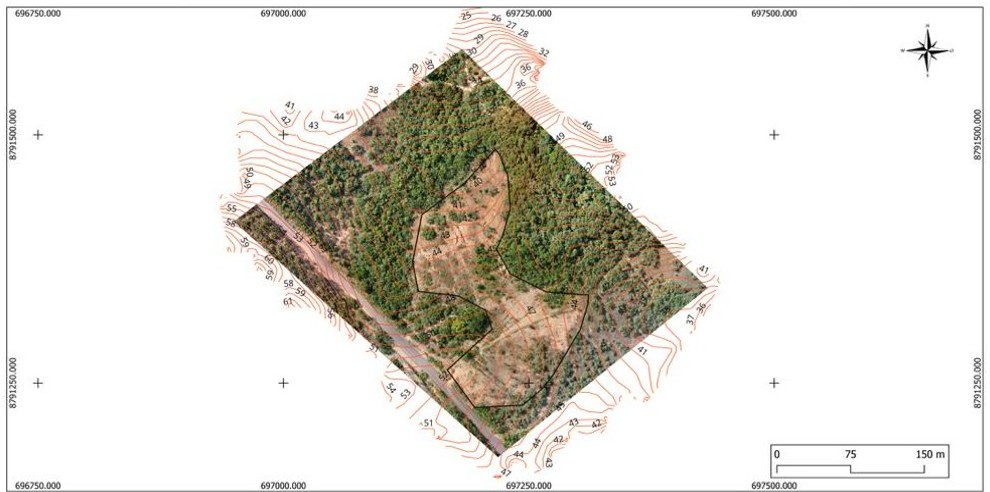
\includegraphics[width=0.75\linewidth,height=\textheight,keepaspectratio]{capitulos/../img/ravina_campo.jpg}

}

\caption{\label{fig-ravina-campo}Ravina ativa em solo tropical --- canal
permanente que não pode ser eliminado por operações agrícolas
convencionais.}

\end{figure}%

As ravinas podem ser classificadas segundo seu mecanismo de crescimento
dominante. As ravinas de cabeceira retrocedem por erosão remontante, na
qual o escoamento concentrado escava a montante, alargando
progressivamente a área de contribuição. As ravinas laterais se expandem
por solapamento e desabamento das paredes, processo acelerado pelo
umedecimento diferencial e pela ação do gelo em altas altitudes ou pela
simples saturação em ambientes tropicais. As ravinas de fundo se
aprofundam por incisão do talvegue, podendo atingir horizontes mais
compactos ou o lençol freático. É comum que os três mecanismos atuem
simultaneamente na mesma ravina, exigindo um tratamento integrado de
bioengenharia que aborde cabeceira, paredes e fundo do canal.

\subsection{Voçorocas}\label{vouxe7orocas}

As voçorocas são feições erosivas de grande porte (profundidade
\textgreater{} 1,5 m, largura \textgreater{} 3 m) que frequentemente
atingem o lençol freático, adicionando a contribuição de água
subterrânea ao processo erosivo. Representam o estágio mais severo de
degradação do solo e constituem um dos maiores desafios para a
bioengenharia.

A formação de voçorocas está associada a três mecanismos
interconectados. O primeiro é a progressão da erosão superficial, na
qual ravinas não controladas se ampliam e aprofundam até atingir
dimensões de voçoroca. O segundo é a erosão subsuperficial
(\emph{piping}), na qual a percolação de água através de
descontinuidades do solo (fraturas, raízes mortas, galerias de animais)
gera túneis internos cujo colapso súbito forma a feição erosiva. O
terceiro é a instabilidade de taludes, na qual o solapamento da base
pela exfiltração do lençol freático causa desabamentos sucessivos das
paredes, ampliando lateralmente a voçoroca.

\begin{figure}

\centering{

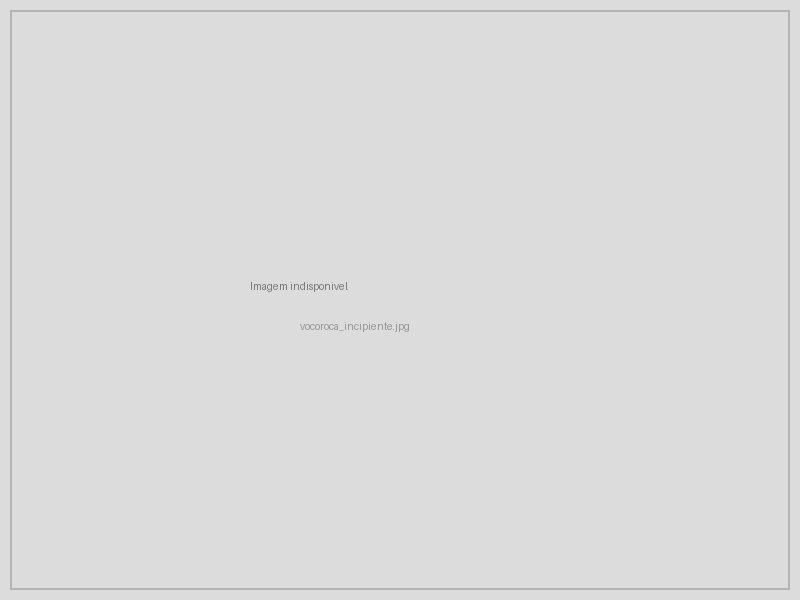
\includegraphics[width=0.75\linewidth,height=\textheight,keepaspectratio]{capitulos/../img/vocoroca_incipiente.jpg}

}

\caption{\label{fig-vocoroca-incipiente}Voçoroca incipiente --- estágio
inicial de formação, quando a ravina começa a ampliar-se e
aprofundar-se, ainda passível de controle por técnicas combinadas de
bioengenharia.}

\end{figure}%

O tratamento de voçorocas ativas exige um projeto integrado que combine
drenagem superficial (desvio das águas de contribuição), drenagem
subsuperficial (interceptação de \emph{pipes}), estabilização mecânica
das paredes (gabiões vivos, paredes Krainer, retaludamento) e
revegetação progressiva. Abordagens pontuais ou parciais tendem ao
fracasso, pois os processos atuantes são múltiplos e interconectados.

\section{Mecanismos de Erosão}\label{mecanismos-de-erosuxe3o}

O processo erosivo envolve três fases sequenciais cujo entendimento é
fundamental para projetar intervenções eficazes.

\subsection{\texorpdfstring{1. Desprendimento
(\emph{Detachment})}{1. Desprendimento (Detachment)}}\label{desprendimento-detachment}

O impacto das gotas de chuva (\emph{splash}) é o principal agente de
desprendimento de partículas de solo. Para dimensionar essa magnitude,
considere que uma gota de 5 mm de diâmetro (comum em chuvas convectivas
tropicais) atinge o solo a aproximadamente 9 m/s, exercendo pressão
instantânea de até 6 MPa (equivalente a cerca de 60 atmosferas), força
suficiente para desagregar partículas e projetá-las a mais de 1 metro de
distância. Uma chuva tropical intensa pode gerar milhares de impactos
por centímetro quadrado por hora.

A taxa de desprendimento é função da energia cinética da chuva:

\[
D_r = K_I \cdot I^2
\]

onde \(D_r\) é a taxa de desprendimento (kg m⁻² s⁻¹), \(K_I\) é a
erodibilidade intergoticular (propriedade do solo) e \(I\) é a
intensidade da chuva (mm h⁻¹). O expoente quadrático indica que a
duplicação da intensidade da chuva quadruplica o desprendimento, o que
explica por que as chuvas tropicais de curta duração e alta intensidade
são tão erosivas.

A proteção contra o desprendimento é a primeira linha de defesa da
bioengenharia. A cobertura vegetal (viva ou morta) intercepta as gotas
de chuva antes que atinjam o solo, eliminando o efeito \emph{splash}.
Uma cobertura de 70\% da superfície reduz o desprendimento em mais de
90\%.

\subsection{2. Transporte}\label{transporte}

As partículas desprendidas são transportadas pelo escoamento
superficial. A capacidade de transporte (\(T_c\)) determina a quantidade
máxima de sedimento que o fluxo pode carregar e depende diretamente da
velocidade e da profundidade do escoamento:

\[
T_c = k_t \cdot \tau^{1.5}
\]

onde \(\tau\) é a tensão cisalhante do fluxo (que depende da velocidade,
profundidade e declividade do escoamento) e \(k_t\) é um coeficiente
empírico que varia com o tamanho das partículas do solo. Essa equação
revela que a redução da velocidade do escoamento (por meio de obstáculos
como paliçadas, cordões vegetativos ou bacias de contenção) é a
estratégia mais eficaz para limitar o transporte de sedimentos.

\subsection{3. Deposição}\label{deposiuxe7uxe3o}

Quando a capacidade de transporte diminui (por redução de velocidade ou
declividade), as partículas em suspensão são depositadas. A deposição é
seletiva quanto ao tamanho das partículas: partículas grossas (areia)
são depositadas primeiro, seguidas por partículas intermediárias
(silte), enquanto partículas finas (argila) podem ser transportadas por
quilômetros até atingir corpos d'água. Esse fenômeno de seletividade
granulométrica explica por que as paliçadas e bacias de sedimentação são
eficazes para reter areia e silte, mas têm eficácia limitada para argila
em suspensão.

\section{Erosão em Regiões
Tropicais}\label{erosuxe3o-em-regiuxf5es-tropicais}

A erosão nas regiões tropicais apresenta particularidades que a
distinguem dos processos erosivos em outras zonas climáticas e que devem
ser consideradas no projeto de bioengenharia. A
Figura~\ref{fig-mapa-erosao} ilustra um mapa de susceptibilidade à
erosão, ferramenta fundamental para o planejamento espacial das
intervenções.

\begin{figure}

\centering{

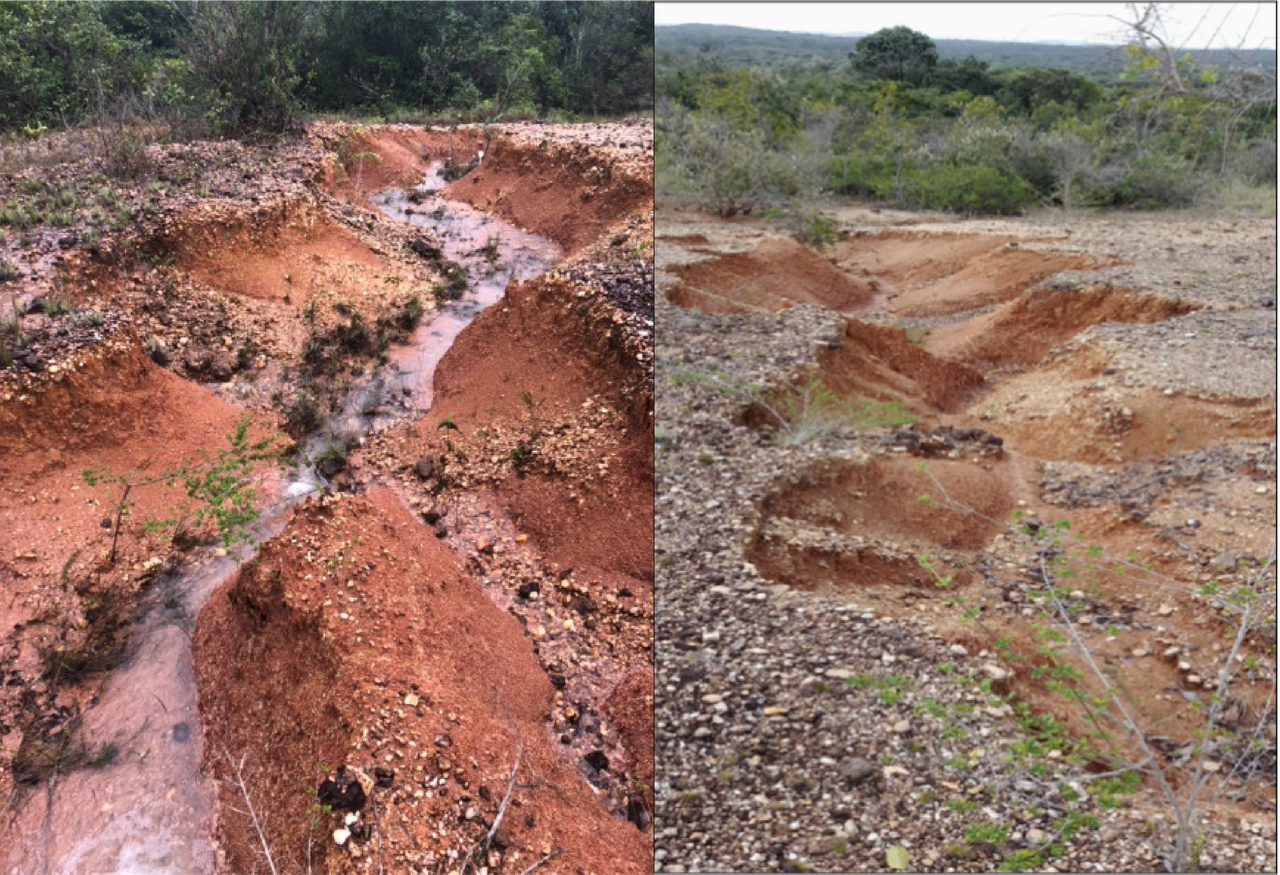
\includegraphics[width=0.85\linewidth,height=\textheight,keepaspectratio]{capitulos/../img/mapa_erosao.png}

}

\caption{\label{fig-mapa-erosao}Mapa de susceptibilidade à erosão e
capacidade de uso do solo --- ferramenta fundamental para planejamento
de intervenções de bioengenharia.}

\end{figure}%

Mapas como o da Figura~\ref{fig-mapa-erosao} são construídos a partir do
cruzamento de informações topográficas (modelo digital de elevação),
pedológicas (classes de solo e erodibilidade), climáticas (erosividade
da chuva) e de uso do solo (cobertura vegetal), e permitem identificar
as áreas prioritárias para intervenção (hotspots erosivos) e dimensionar
as técnicas mais adequadas para cada zona.

\begin{figure}

\centering{

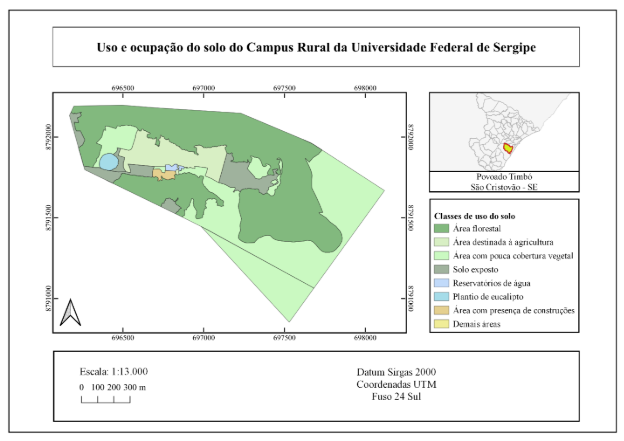
\includegraphics[width=0.85\linewidth,height=\textheight,keepaspectratio]{capitulos/../img/mapa_uso_solo.png}

}

\caption{\label{fig-mapa-uso-solo}Mapa de uso e cobertura do solo ---
classificação das categorias de uso da terra que alimenta o fator \(C\)
da RUSLE e o parâmetro \(CN\) do método SCS, essenciais para o
dimensionamento de intervenções de bioengenharia.}

\end{figure}%

\begin{tcolorbox}[enhanced jigsaw, leftrule=.75mm, colframe=quarto-callout-important-color-frame, colback=white, bottomrule=.15mm, opacityback=0, colbacktitle=quarto-callout-important-color!10!white, breakable, bottomtitle=1mm, opacitybacktitle=0.6, title=\textcolor{quarto-callout-important-color}{\faExclamation}\hspace{0.5em}{Particularidades tropicais}, titlerule=0mm, toprule=.15mm, toptitle=1mm, rightrule=.15mm, left=2mm, arc=.35mm, coltitle=black]

Nas regiões tropicais, quatro fatores condicionam a intensidade e a
dinâmica dos processos erosivos. Primeiro, a elevada erosividade das
chuvas, com \(EI_{30}\) superior a 10.000 MJ mm ha⁻¹ h⁻¹ ano⁻¹ (contra
1.000--3.000 em zonas temperadas), concentrada em poucos meses da
estação chuvosa. Segundo, os solos com coesão aparente, que se mostram
estáveis quando secos mas colapsam quando saturados, gerando rupturas
súbitas e imprevisíveis. Terceiro, a ocorrência frequente de erosão
subsuperficial (\emph{piping}), especialmente em solos com gradiente
textural (Argissolos) ou com camadas de impedimento (Plintossolos), que
gera túneis subterrâneos cujo colapso forma ravinas e voçorocas. Quarto,
os ciclos repetitivos de umedecimento e secagem, que causam fissuração
superficial, criando caminhos preferenciais para infiltração concentrada
e acelerando a desagregação do solo.

\end{tcolorbox}

\begin{figure}

\centering{

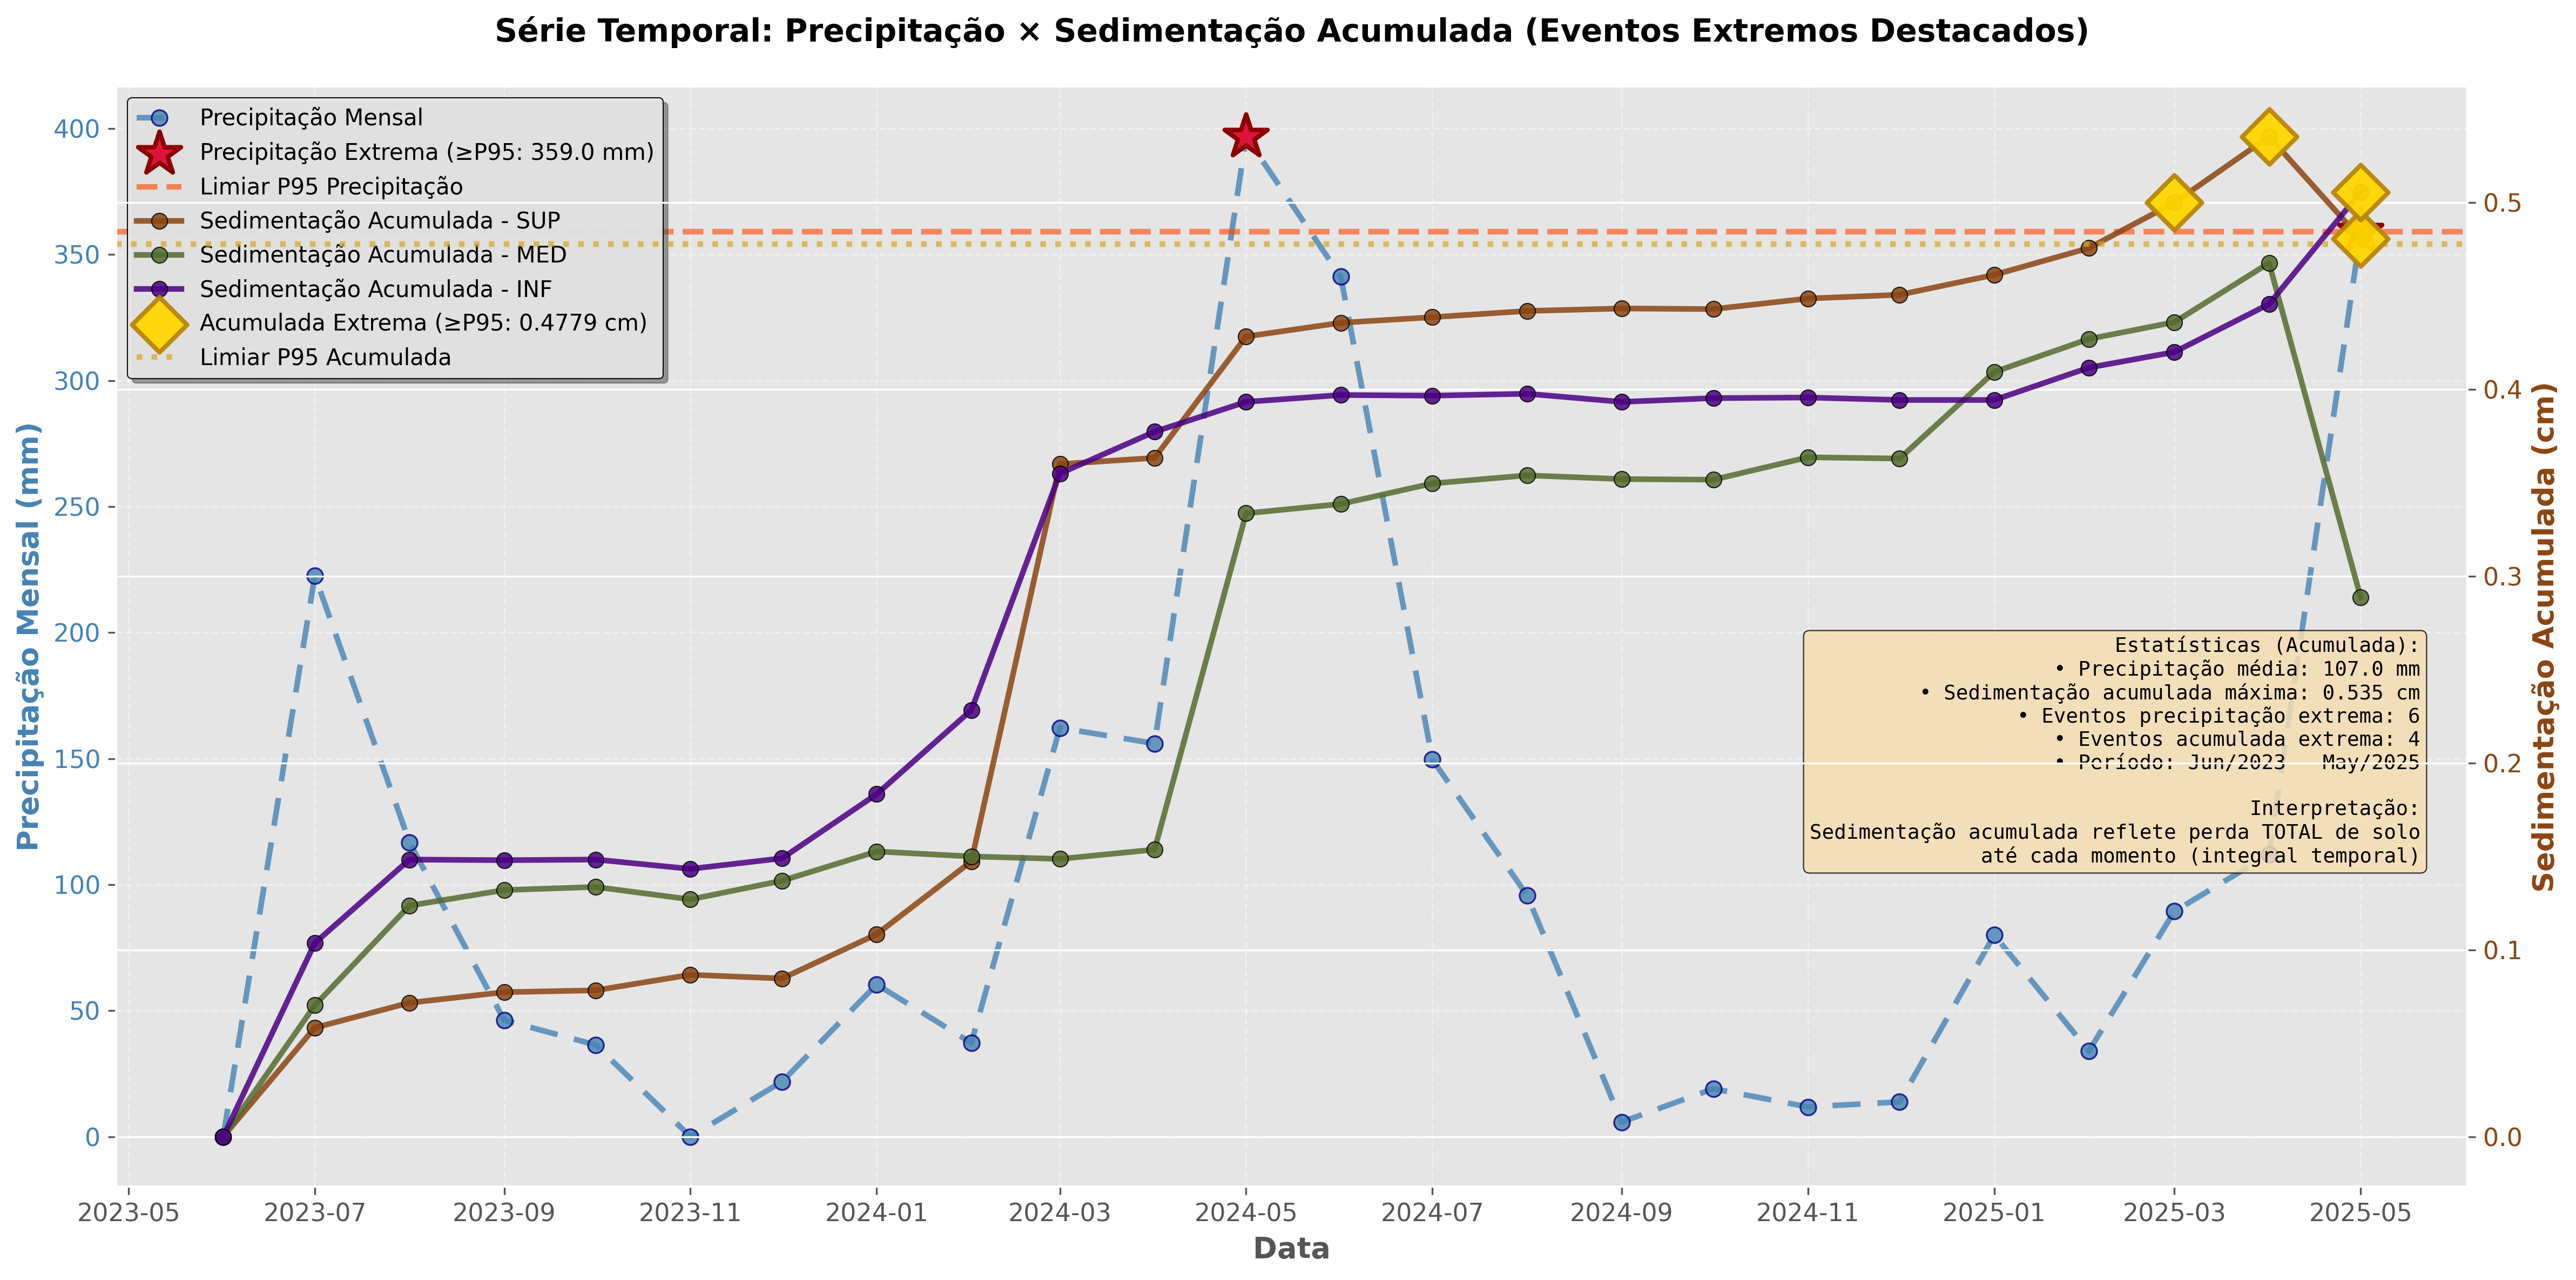
\includegraphics[width=0.8\linewidth,height=\textheight,keepaspectratio]{capitulos/../img/eventos_extremos.png}

}

\caption{\label{fig-eventos-extremos}Eventos climáticos extremos e
erosão --- a intensificação de chuvas convectivas tropicais aumenta a
erosividade e a frequência de rupturas em encostas e margens fluviais.}

\end{figure}%

\section{Erosão Marginal}\label{erosuxe3o-marginal}

Em regiões tropicais, a erosão das margens fluviais é um processo
crítico que afeta diretamente comunidades ribeirinhas, áreas agrícolas,
infraestrutura viária e ecossistemas ripários. O mecanismo envolve o
solapamento da base da margem pelo fluxo do rio (que remove material na
zona de contato com a água), seguido pelo desabamento gravitacional do
bloco superior, ciclo que se repete a cada cheia. O Baixo São Francisco
(SE/AL), por exemplo, perde em média 2 a 5 metros de margem por ano, com
registro de trechos onde a erosão atingiu 10 m/ano, resultando em perda
de terras agriculturáveis, destruição de residências e desestabilização
de rodovias.

A bioengenharia de solos oferece soluções específicas para erosão
marginal, combinando retaludamento (suavização do ângulo da margem para
estabilização geométrica), enrocamento vegetado na base da margem
(resistência mecânica à abrasão pelo fluxo com enraizamento progressivo)
e revegetação ciliar no topo do talude (ancoragem radicular e
interceptação de escoamento superficial). Essas técnicas serão
detalhadas nos capítulos sobre gabiões vivos
(\textbf{?@sec-gabiao-vivo}), paredes Krainer
(\textbf{?@sec-parede-krainer}) e revegetação
(\textbf{?@sec-revegetacao}).

\section{Tolerância de Perda de
Solo}\label{toleruxe2ncia-de-perda-de-solo}

A tolerância de perda de solo (\(T\)) é um conceito fundamental para
justificar a necessidade de intervenções de bioengenharia. Trata-se da
taxa máxima de erosão compatível com a manutenção da produtividade do
solo em longo prazo, ou seja, a taxa na qual a formação de novo solo
(por intemperismo) equilibra a perda por erosão.

\begin{longtable}[]{@{}
  >{\raggedright\arraybackslash}p{(\linewidth - 4\tabcolsep) * \real{0.3061}}
  >{\raggedright\arraybackslash}p{(\linewidth - 4\tabcolsep) * \real{0.3878}}
  >{\raggedright\arraybackslash}p{(\linewidth - 4\tabcolsep) * \real{0.3061}}@{}}
\caption{Tolerância de perda de solo para classes de solos tropicais
(Bertoni \& Lombardi Neto, 2017).}\label{tbl-tolerancia}\tabularnewline
\toprule\noalign{}
\begin{minipage}[b]{\linewidth}\raggedright
Classe de solo
\end{minipage} & \begin{minipage}[b]{\linewidth}\raggedright
T (t ha⁻¹ ano⁻¹)
\end{minipage} & \begin{minipage}[b]{\linewidth}\raggedright
Justificativa
\end{minipage} \\
\midrule\noalign{}
\endfirsthead
\toprule\noalign{}
\begin{minipage}[b]{\linewidth}\raggedright
Classe de solo
\end{minipage} & \begin{minipage}[b]{\linewidth}\raggedright
T (t ha⁻¹ ano⁻¹)
\end{minipage} & \begin{minipage}[b]{\linewidth}\raggedright
Justificativa
\end{minipage} \\
\midrule\noalign{}
\endhead
\bottomrule\noalign{}
\endlastfoot
Solos profundos (Latossolos) & 9--12 & Manto espesso permite maior perda
sem comprometer a raiz \\
Solos moderadamente profundos & 5--9 & Equilíbrio entre profundidade e
taxa de formação \\
Solos rasos (Neossolos) & 2--5 & Qualquer perda compromete rapidamente a
capacidade produtiva \\
\end{longtable}

Quando a perda atual (\(A\), calculada pela RUSLE ou medida em parcelas
experimentais) excede a tolerância (\(T\)), intervenções de
bioengenharia são necessárias para evitar a degradação irreversível do
recurso solo. Essa relação \(A > T\) é o critério técnico que fundamenta
a recomendação de intervenção e orienta o dimensionamento das técnicas
de controle, cuja intensidade deve ser proporcional ao excedente
\(A - T\).

\chapter{Importância da
Classificação}\label{importuxe2ncia-da-classificauxe7uxe3o}

\# Classificação de Feições Erosivas \{\#sec-classificacao-feicoes\}

A classificação precisa das feições erosivas é o primeiro passo para o
dimensionamento de intervenções de bioengenharia. Sem uma classificação
rigorosa, corre-se o risco de subdimensionar o tratamento (aplicar uma
solução simples a um problema complexo, resultando em falha) ou de
superdimensioná-lo (gastar recursos desnecessários com técnicas
sofisticadas onde uma solução simples bastaria). Uma ravina de cabeceira
com 0,5 m de profundidade demanda técnicas completamente diferentes de
uma voçoroca com 8 m de profundidade e contribuição do lençol freático,
embora ambas sejam ``feições erosivas''.

O mapeamento das feições erosivas pode ser realizado por diferentes
métodos, desde o reconhecimento visual em campo até o uso de tecnologias
de sensoriamento remoto. A Figura~\ref{fig-foto-aerea} demonstra a
capacidade dos sistemas RPAS (Remotely Piloted Aircraft Systems,
popularmente chamados drones) para identificar e mapear feições erosivas
com resolução espacial centimétrica.

\begin{figure}

\centering{

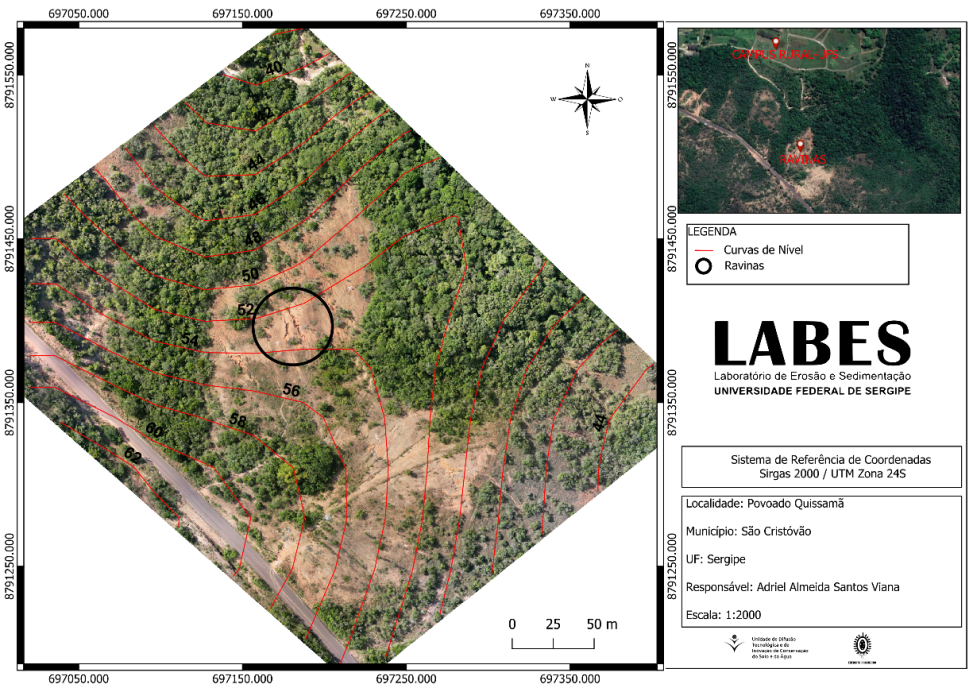
\includegraphics[width=0.85\linewidth,height=\textheight,keepaspectratio]{capitulos/../img/foto_aerea.png}

}

\caption{\label{fig-foto-aerea}Visão aérea de feições erosivas --- o
mapeamento por RPAS permite identificar e classificar ravinas com
precisão espacial centimétrica.}

\end{figure}%

A partir de imagens como a da Figura~\ref{fig-foto-aerea}, é possível
extrair informações geométricas detalhadas (largura, profundidade,
comprimento, área da seção transversal) que alimentam os sistemas de
classificação e orientam a seleção de técnicas de bioengenharia.

\section{Elementary Gully Classification
(EGC)}\label{elementary-gully-classification-egc}

O sistema Elementary Gully Classification (EGC) é uma abordagem
sistemática que permite classificar feições erosivas com base em suas
características geométricas e hidráulicas, utilizando dados obtidos por
levantamento topográfico convencional, GNSS de precisão ou sensoriamento
remoto (drone/VANT). A vantagem do EGC é fornecer critérios
quantitativos e objetivos para distinguir entre classes de feições,
substituindo classificações subjetivas baseadas apenas na impressão
visual do observador.

\subsection{Parâmetros Geométricos}\label{paruxe2metros-geomuxe9tricos}

Para classificar uma feição erosiva pelo EGC, é necessário medir seis
parâmetros fundamentais, descritos na Tabela~\ref{tbl-parametros}. Esses
parâmetros podem ser obtidos tanto em campo (com trena, nível óptico ou
estação total) quanto a partir do modelo digital de superfície gerado
por levantamento com drone.

\begin{longtable}[]{@{}
  >{\raggedright\arraybackslash}p{(\linewidth - 6\tabcolsep) * \real{0.2558}}
  >{\raggedright\arraybackslash}p{(\linewidth - 6\tabcolsep) * \real{0.2093}}
  >{\raggedright\arraybackslash}p{(\linewidth - 6\tabcolsep) * \real{0.2558}}
  >{\raggedright\arraybackslash}p{(\linewidth - 6\tabcolsep) * \real{0.2791}}@{}}
\caption{Parâmetros geométricos para classificação de feições
erosivas.}\label{tbl-parametros}\tabularnewline
\toprule\noalign{}
\begin{minipage}[b]{\linewidth}\raggedright
Parâmetro
\end{minipage} & \begin{minipage}[b]{\linewidth}\raggedright
Símbolo
\end{minipage} & \begin{minipage}[b]{\linewidth}\raggedright
Descrição
\end{minipage} & \begin{minipage}[b]{\linewidth}\raggedright
Como medir
\end{minipage} \\
\midrule\noalign{}
\endfirsthead
\toprule\noalign{}
\begin{minipage}[b]{\linewidth}\raggedright
Parâmetro
\end{minipage} & \begin{minipage}[b]{\linewidth}\raggedright
Símbolo
\end{minipage} & \begin{minipage}[b]{\linewidth}\raggedright
Descrição
\end{minipage} & \begin{minipage}[b]{\linewidth}\raggedright
Como medir
\end{minipage} \\
\midrule\noalign{}
\endhead
\bottomrule\noalign{}
\endlastfoot
Largura & \(W\) & Distância entre bordas (m) & Trena ou perfil
transversal do MDS \\
Profundidade & \(D\) & Distância vertical da borda ao fundo (m) & Mira
topográfica ou diferença altimétrica do MDS \\
Comprimento & \(L\) & Extensão longitudinal (m) & Trena ou polyline
sobre ortomosaico \\
Área da seção & \(A_s\) & Área da seção transversal (m²) & Cálculo por
integração do perfil \\
Razão W/D & --- & Indicador da forma da seção (V, U ou trapezoidal) &
Divisão de W por D \\
Declividade do fundo & \(S_f\) & Gradiente longitudinal (\%) & Nível
óptico ou perfil longitudinal do MDT \\
\end{longtable}

A razão W/D é particularmente informativa. Feições com W/D \textless{} 1
(mais profundas que largas) indicam erosão concentrada ativa com
aprofundamento dominante, enquanto feições com W/D \textgreater{} 3
(mais largas que profundas) sugerem alargamento por desabamento das
paredes, frequentemente associado à contribuição do lençol freático.
Essa distinção orienta a seleção de técnicas: feições profundas e
estreitas respondem bem a paliçadas e check-dams, enquanto feições
largas e rasas demandam tratamento de paredes (retaludamento, biomantas,
revegetação).

\subsection{Classificação por
Dimensões}\label{classificauxe7uxe3o-por-dimensuxf5es}

A Tabela~\ref{tbl-dimensoes} apresenta os critérios dimensionais para
cada classe de feição erosiva. Os limites entre classes não são
arbitrários; refletem transições nos processos dominantes e,
consequentemente, nas técnicas de controle recomendadas.

\begin{longtable}[]{@{}
  >{\raggedright\arraybackslash}p{(\linewidth - 8\tabcolsep) * \real{0.1250}}
  >{\raggedright\arraybackslash}p{(\linewidth - 8\tabcolsep) * \real{0.2031}}
  >{\raggedright\arraybackslash}p{(\linewidth - 8\tabcolsep) * \real{0.1406}}
  >{\raggedright\arraybackslash}p{(\linewidth - 8\tabcolsep) * \real{0.2344}}
  >{\raggedright\arraybackslash}p{(\linewidth - 8\tabcolsep) * \real{0.2969}}@{}}
\caption{Classificação de feições erosivas por dimensões e processo
dominante.}\label{tbl-dimensoes}\tabularnewline
\toprule\noalign{}
\begin{minipage}[b]{\linewidth}\raggedright
Classe
\end{minipage} & \begin{minipage}[b]{\linewidth}\raggedright
Profundidade
\end{minipage} & \begin{minipage}[b]{\linewidth}\raggedright
Largura
\end{minipage} & \begin{minipage}[b]{\linewidth}\raggedright
Área de seção
\end{minipage} & \begin{minipage}[b]{\linewidth}\raggedright
Processo dominante
\end{minipage} \\
\midrule\noalign{}
\endfirsthead
\toprule\noalign{}
\begin{minipage}[b]{\linewidth}\raggedright
Classe
\end{minipage} & \begin{minipage}[b]{\linewidth}\raggedright
Profundidade
\end{minipage} & \begin{minipage}[b]{\linewidth}\raggedright
Largura
\end{minipage} & \begin{minipage}[b]{\linewidth}\raggedright
Área de seção
\end{minipage} & \begin{minipage}[b]{\linewidth}\raggedright
Processo dominante
\end{minipage} \\
\midrule\noalign{}
\endhead
\bottomrule\noalign{}
\endlastfoot
Sulco & \textless{} 0,3 m & \textless{} 0,3 m & \textless{} 0,09 m² &
Escoamento difuso concentrado \\
Ravina pequena & 0,3--1,0 m & 0,3--1,0 m & 0,09--1,0 m² & Escoamento
concentrado com incisão \\
Ravina média & 1,0--3,0 m & 1,0--5,0 m & 1,0--15 m² & Escoamento
concentrado + solapamento \\
Ravina grande & 3,0--5,0 m & 5,0--15 m & 15--75 m² & Múltiplos processos
superficiais \\
Voçoroca & \textgreater{} 5,0 m & \textgreater{} 15 m & \textgreater{}
75 m² & Superficial + subsuperficial + gravitacional \\
\end{longtable}

\section{Levantamento com VANT
(Drone)}\label{levantamento-com-vant-drone}

O uso de Veículos Aéreos Não Tripulados (VANT/drone) revolucionou o
levantamento de feições erosivas nas últimas duas décadas. Antes dos
drones, o mapeamento detalhado de ravinas e voçorocas exigia
levantamentos topográficos de campo laboriosos, custosos e, em muitos
casos, perigosos (trabalhar dentro de voçorocas ativas envolve risco de
desabamento). Com os drones, é possível obter modelos tridimensionais de
alta resolução a partir de sobrevoos de poucos minutos, sem expor
operadores a riscos.

As imagens a seguir ilustram dois aspectos complementares do
levantamento. A Figura~\ref{fig-ravina-detalhe} mostra o detalhe de uma
ravina em resolução que permite medir os parâmetros geométricos da
Tabela~\ref{tbl-parametros} diretamente no modelo digital, enquanto a
Figura~\ref{fig-perfil-feicoes} revela os horizontes do solo expostos
pela erosão, informação essencial para dimensionar a profundidade de
ancoragem das estruturas de bioengenharia.

\begin{figure}

\begin{minipage}{0.50\linewidth}

\begin{figure}[H]

\centering{

\pandocbounded{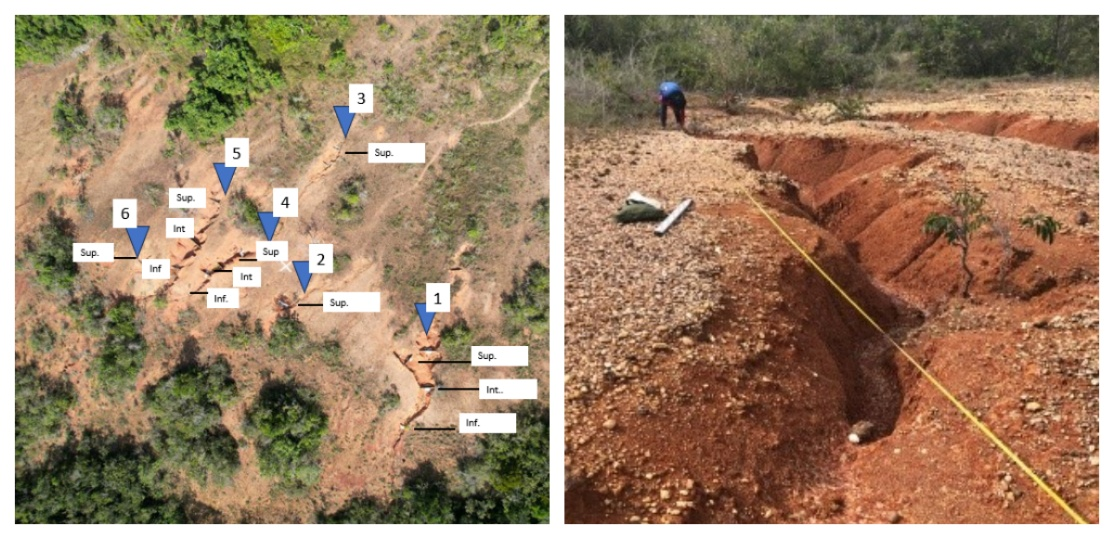
\includegraphics[keepaspectratio]{capitulos/../img/ravina_detalhe.jpg}}

}

\caption{\label{fig-ravina-detalhe}Detalhe de ravina --- parâmetros
geométricos podem ser medidos em campo ou pelo modelo digital gerado por
drone.}

\end{figure}%

\end{minipage}%
%
\begin{minipage}{0.50\linewidth}

\begin{figure}[H]

\centering{

\pandocbounded{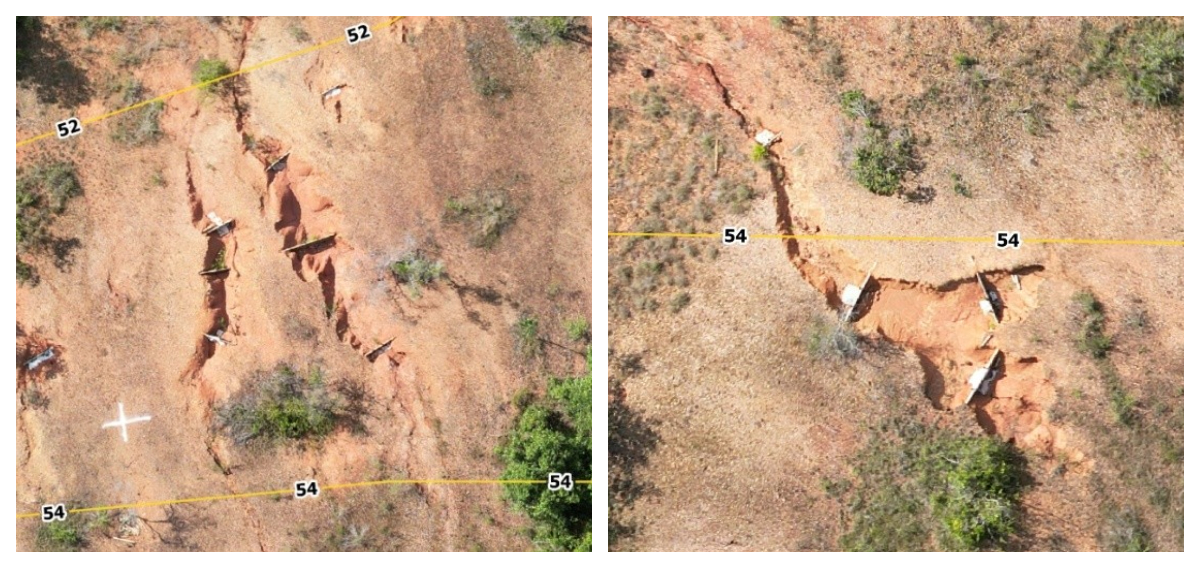
\includegraphics[keepaspectratio]{capitulos/../img/perfil_solo_feicoes.jpg}}

}

\caption{\label{fig-perfil-feicoes}Perfil de solo exposto pela erosão
--- a análise dos horizontes auxilia no dimensionamento das
intervenções.}

\end{figure}%

\end{minipage}%

\end{figure}%

\subsection{Fluxo de Trabalho com
VANT}\label{fluxo-de-trabalho-com-vant}

O levantamento com VANT segue uma sequência operacional padronizada em
cinco etapas. A primeira etapa é o planejamento de voo, no qual se
define a área de cobertura, a altitude de voo (tipicamente 50--100 m
acima do terreno, resultando em resolução de 1--3 cm/pixel) e a
sobreposição entre imagens (mínimo de 80\% frontal e 60\% lateral para
garantir a reconstrução tridimensional). A segunda etapa é a
distribuição de pontos de controle (GCPs, \emph{Ground Control Points}),
que são alvos georreferenciados com GNSS RTK (precisão centimétrica)
distribuídos pela área de interesse para garantir a acurácia posicional
do modelo.

A terceira etapa é o processamento fotogramétrico, realizado por
softwares de \emph{Structure from Motion} (SfM) como Agisoft Metashape,
OpenDroneMap ou Pix4D, que reconstroem a geometria tridimensional da
cena a partir da sobreposição das centenas de fotografias obtidas pelo
drone. O resultado é uma nuvem densa de pontos tridimensionais com
milhões de coordenadas XYZ. A quarta etapa é a geração de produtos
cartográficos, incluindo o ortomosaico (imagem georreferenciada em
projeção ortogonal), o MDS (Modelo Digital de Superfície, que inclui a
vegetação), o MDT (Modelo Digital do Terreno, obtido pela filtragem da
vegetação) e as curvas de nível. Por fim, a quinta etapa é a análise
geomorfológica, na qual se extraem seções transversais das feições,
calculam-se volumes de perda ou deposição de solo por diferença de MDTs
multitemporais e se quantificam taxas de recuo de cabeceira e de
alargamento lateral.

\section{Seleção de Técnicas por
Classe}\label{seleuxe7uxe3o-de-tuxe9cnicas-por-classe}

A classificação da feição erosiva orienta diretamente a seleção das
técnicas de bioengenharia, conforme sintetizado na
Tabela~\ref{tbl-selecao}. A lógica é progressiva: quanto maior e mais
complexa a feição, maior o número e a sofisticação das técnicas
combinadas.

\begin{longtable}[]{@{}
  >{\raggedright\arraybackslash}p{(\linewidth - 4\tabcolsep) * \real{0.1739}}
  >{\raggedright\arraybackslash}p{(\linewidth - 4\tabcolsep) * \real{0.3696}}
  >{\raggedright\arraybackslash}p{(\linewidth - 4\tabcolsep) * \real{0.4565}}@{}}
\caption{Seleção de técnicas de bioengenharia por classe de feição
erosiva.}\label{tbl-selecao}\tabularnewline
\toprule\noalign{}
\begin{minipage}[b]{\linewidth}\raggedright
Classe
\end{minipage} & \begin{minipage}[b]{\linewidth}\raggedright
Técnica primária
\end{minipage} & \begin{minipage}[b]{\linewidth}\raggedright
Técnica complementar
\end{minipage} \\
\midrule\noalign{}
\endfirsthead
\toprule\noalign{}
\begin{minipage}[b]{\linewidth}\raggedright
Classe
\end{minipage} & \begin{minipage}[b]{\linewidth}\raggedright
Técnica primária
\end{minipage} & \begin{minipage}[b]{\linewidth}\raggedright
Técnica complementar
\end{minipage} \\
\midrule\noalign{}
\endhead
\bottomrule\noalign{}
\endlastfoot
Sulco & Cobertura vegetal, palhada & Cordões vegetativos \\
Ravina pequena & Paliçadas de bambu & Revegetação \\
Ravina média & Paliçadas + check-dams & Hidrossemeadura \\
Ravina grande & Gabião vivo & Biomantas + drenagem \\
Voçoroca & Projeto integrado (retaludamento + drenagem + gabião +
revegetação) & Parede Krainer, enrocamento \\
\end{longtable}

\begin{tcolorbox}[enhanced jigsaw, leftrule=.75mm, colframe=quarto-callout-tip-color-frame, colback=white, bottomrule=.15mm, opacityback=0, colbacktitle=quarto-callout-tip-color!10!white, breakable, bottomtitle=1mm, opacitybacktitle=0.6, title=\textcolor{quarto-callout-tip-color}{\faLightbulb}\hspace{0.5em}{Regra prática}, titlerule=0mm, toprule=.15mm, toptitle=1mm, rightrule=.15mm, left=2mm, arc=.35mm, coltitle=black]

Quanto maior a feição erosiva, maior a necessidade de combinação de
técnicas e de um projeto integrado que considere drenagem, estabilização
mecânica e revegetação simultaneamente. Feições pequenas (sulcos e
ravinas pequenas) podem ser tratadas com uma única técnica, enquanto
voçorocas sempre exigem projeto multidisciplinar envolvendo drenagem,
estabilização e revegetação coordenadas.

\end{tcolorbox}

\section{Monitoramento Temporal}\label{monitoramento-temporal}

O monitoramento periódico das feições erosivas é essencial para avaliar
a eficácia das intervenções de bioengenharia e tomar decisões de
manutenção ou reforço. Sem monitoramento, é impossível saber se a
intervenção está funcionando até que uma eventual falha se manifeste de
forma catastrófica. A frequência mínima recomendada é trimestral durante
os dois primeiros anos após a implantação e semestral a partir do
terceiro ano.

Os indicadores-chave que devem ser medidos em cada campanha de
monitoramento são a taxa de recuo da cabeceira (m/ano, esperando-se
estabilização ou redução progressiva), a taxa de alargamento lateral
(m/ano, que indica se as paredes estão sendo estabilizadas), o volume de
sedimento retido nas estruturas (m³, medido pela diferença de cota a
montante das paliçadas ou check-dams), a cobertura vegetal no interior
da feição (\%, que deve aumentar progressivamente) e a estabilidade das
paredes laterais (ângulo do talude, monitorado por seções transversais).

A comparação de MDTs obtidos por drone em campanhas sucessivas permite
calcular com precisão os volumes de perda e deposição de solo,
identificando espacialmente as zonas ativas (ainda em erosão) e as zonas
estabilizadas (com deposição e revegetação), orientando ações corretivas
focalizadas.

\section{Tecnologias Emergentes de
Monitoramento}\label{tecnologias-emergentes-de-monitoramento}

O avanço das tecnologias de sensoriamento e comunicação sem fio ampliou
significativamente o arsenal de ferramentas disponíveis para o
monitoramento de feições erosivas e da eficácia de intervenções de
bioengenharia. Três tecnologias emergentes merecem destaque por seu
potencial de aplicação em condições tropicais.

\subsection{Sensores IoT para Monitoramento
Contínuo}\label{sensores-iot-para-monitoramento-contuxednuo}

A Internet das Coisas (\emph{Internet of Things}, IoT) permite a
instalação de redes de sensores autônomos em campo, capazes de
transmitir dados em tempo real via rede celular (GSM/4G), LoRaWAN ou
satélite. Em projetos de bioengenharia, sensores de umidade volumétrica
do solo (TDR ou capacitivos) instalados em diferentes profundidades ao
longo de perfis transversais à feição erosiva permitem monitorar
continuamente a frente de umedecimento durante eventos de chuva,
identificando o momento em que a saturação atinge a zona crítica de
ruptura. Piezômetros automatizados registram a variação do nível do
lençol freático com resolução temporal de minutos, dado essencial para a
previsão de instabilidades em voçorocas com contribuição de água
subterrânea. Inclinômetros MEMS (\emph{Micro-Electro-Mechanical
Systems}) detectam deslocamentos milimétricos nas paredes laterais de
feições erosivas, funcionando como sistemas de alerta precoce para
desabamentos. Pluviógrafos de báscula conectados à mesma rede permitem
correlacionar diretamente a intensidade da chuva com a resposta
hidrológica do solo monitorado, alimentando modelos preditivos de erosão
em tempo real.

A Tabela~\ref{tbl-iot} sintetiza os sensores recomendados para um
sistema de monitoramento IoT aplicado a projetos de bioengenharia.

\begin{longtable}[]{@{}
  >{\raggedright\arraybackslash}p{(\linewidth - 6\tabcolsep) * \real{0.1739}}
  >{\raggedright\arraybackslash}p{(\linewidth - 6\tabcolsep) * \real{0.3478}}
  >{\raggedright\arraybackslash}p{(\linewidth - 6\tabcolsep) * \real{0.2391}}
  >{\raggedright\arraybackslash}p{(\linewidth - 6\tabcolsep) * \real{0.2391}}@{}}
\caption{Sensores IoT para monitoramento de projetos de
bioengenharia.}\label{tbl-iot}\tabularnewline
\toprule\noalign{}
\begin{minipage}[b]{\linewidth}\raggedright
Sensor
\end{minipage} & \begin{minipage}[b]{\linewidth}\raggedright
Variável medida
\end{minipage} & \begin{minipage}[b]{\linewidth}\raggedright
Resolução
\end{minipage} & \begin{minipage}[b]{\linewidth}\raggedright
Aplicação
\end{minipage} \\
\midrule\noalign{}
\endfirsthead
\toprule\noalign{}
\begin{minipage}[b]{\linewidth}\raggedright
Sensor
\end{minipage} & \begin{minipage}[b]{\linewidth}\raggedright
Variável medida
\end{minipage} & \begin{minipage}[b]{\linewidth}\raggedright
Resolução
\end{minipage} & \begin{minipage}[b]{\linewidth}\raggedright
Aplicação
\end{minipage} \\
\midrule\noalign{}
\endhead
\bottomrule\noalign{}
\endlastfoot
TDR ou capacitivo & Umidade volumétrica (\%) & ±1\% & Frente de
umedecimento, infiltração \\
Piezômetro vibrating wire & Nível piezométrico (m) & ±1 mm &
Poropressão, lençol freático \\
Inclinômetro MEMS & Deslocamento angular (°) & ±0,001° & Movimento de
massa, alerta precoce \\
Pluviógrafo de báscula & Precipitação (mm) & 0,2 mm & Correlação
chuva-resposta erosiva \\
Sensor de turbidez óptico & Sedimento em suspensão (NTU) & ±2 NTU &
Carga sólida no exutório \\
\end{longtable}

\subsection{LiDAR Terrestre e
Aerotransportado}\label{lidar-terrestre-e-aerotransportado}

O LiDAR (\emph{Light Detection and Ranging}) complementa a fotogrametria
SfM com a capacidade de penetrar a cobertura vegetal, gerando modelos
digitais de terreno (MDT) sob dosséis florestais fechados, situação em
que a fotogrametria óptica é incapaz de reconstruir a superfície do
solo. Em feições erosivas sob regeneração vegetal avançada, o LiDAR
aerotransportado por drone (resolução de 5--20 pontos/m²) permite
quantificar volumes de preenchimento e deposição que seriam invisíveis
por fotogrametria, sendo particularmente útil no monitoramento de médio
e longo prazo (anos 3--10 após a intervenção). O LiDAR terrestre (TLS,
\emph{Terrestrial Laser Scanner}), com resolução milimétrica
(\textgreater{} 1.000 pontos/m²), é a ferramenta de maior precisão para
quantificar taxas de recuo de cabeceira e evolução de seções
transversais, funcionando como referência para calibração dos demais
métodos.

\subsection{Sensoriamento Distribuído por Fibra
Óptica}\label{sensoriamento-distribuuxeddo-por-fibra-uxf3ptica}

A tecnologia de sensoriamento distribuído por fibra óptica (DFOS,
\emph{Distributed Fiber Optic Sensing}) permite monitorar deformações,
temperatura e umidade ao longo de cabos de fibra óptica enterrados no
maciço de solo, com resolução espacial de 0,5--1,0 m e extensão de até
10 km por canal. Em estruturas de bioengenharia de grande porte (gabiões
vivos, paredes Krainer), a fibra óptica instalada durante a construção
funciona como um ``sistema nervoso'' da estrutura, detectando
deformações diferenciais, variações de temperatura associadas a fluxo
preferencial de água (piping) e mudanças de umidade que indicam
saturação localizada. Embora o custo atual do sistema de aquisição
(interrogador óptico, R\$ 80.000--200.000) limite sua aplicação a obras
de grande responsabilidade (barragens, encostas urbanas), a tendência de
redução de custos torna essa tecnologia cada vez mais acessível para
projetos de pesquisa e monitoramento de referência.

\begin{tcolorbox}[enhanced jigsaw, leftrule=.75mm, colframe=quarto-callout-note-color-frame, colback=white, bottomrule=.15mm, opacityback=0, colbacktitle=quarto-callout-note-color!10!white, breakable, bottomtitle=1mm, opacitybacktitle=0.6, title=\textcolor{quarto-callout-note-color}{\faInfo}\hspace{0.5em}{Integração de dados}, titlerule=0mm, toprule=.15mm, toptitle=1mm, rightrule=.15mm, left=2mm, arc=.35mm, coltitle=black]

A convergência dessas tecnologias em plataformas de gestão de dados
geoespaciais (como GeoNode, QGIS Server ou Google Earth Engine) permite
a criação de painéis de monitoramento (\emph{dashboards}) que integram
dados de sensores IoT, produtos de sensoriamento remoto (drone, LiDAR,
satélite) e modelos hidrológicos em uma interface única de tomada de
decisão, viabilizando a gestão adaptativa preconizada pelos critérios
IUCN para NBS (ver \textbf{?@sec-nbs}).

\end{tcolorbox}

\part{Parte II --- Técnicas de Bioengenharia}

\chapter{Princípios da
Revegetação}\label{princuxedpios-da-revegetauxe7uxe3o}

\# Revegetação e Espécies para Bioengenharia \{\#sec-revegetacao\}

A revegetação é a técnica fundamental e mais antiga da bioengenharia de
solos. Enquanto estruturas como paliçadas, gabiões e paredes Krainer
oferecem estabilização mecânica imediata, é a vegetação que assegura a
proteção em longo prazo, transformando progressivamente uma superfície
vulnerável em um sistema autossustentável. Por essa razão, todas as
demais técnicas de bioengenharia são, em última análise, projetadas para
criar condições favoráveis ao estabelecimento vegetal.

O sistema radicular é o componente-chave dessa proteção. A
Figura~\ref{fig-vetiver-raizes} apresenta o sistema radicular do vetiver
(\emph{Vetiveria zizanioides}), considerado o padrão de referência em
bioengenharia tropical, cujas raízes podem ultrapassar 3 m de
profundidade em solos bem drenados.

\begin{figure}

\centering{

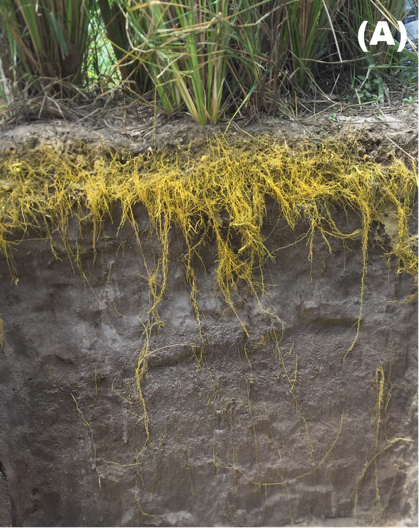
\includegraphics[width=0.7\linewidth,height=\textheight,keepaspectratio]{capitulos/../img/vetiver_1.png}

}

\caption{\label{fig-vetiver-raizes}Sistema radicular de vetiver ---
raízes profundas que conferem coesão e ancoragem ao solo, mecanismo
fundamental da revegetação em bioengenharia.}

\end{figure}%

Conforme ilustrado na Figura~\ref{fig-vetiver-raizes}, a densidade e a
profundidade das raízes do vetiver criam uma malha tridimensional que
reforça mecanicamente o solo. As plantas protegem o solo por seis
mecanismos simultâneos e complementares. A interceptação da energia
cinética das gotas de chuva pela copa e pelas folhas reduz em até 90\% o
impacto direto sobre a superfície, eliminando o efeito \emph{splash}
(desprendimento por impacto). A proteção superficial pelo acúmulo de
serrapilheira (folhas mortas, restos vegetais) cria uma camada
amortecedora que reduz a velocidade do escoamento e protege os agregados
do solo contra desagregação. O reforço radicular aumenta a coesão do
solo em 5--40 kPa, conforme demonstrado pelo modelo de Wu-Waldron
discutido no \textbf{?@sec-solos-tropicais}, sendo o incremento
proporcional à densidade e à resistência à tração das raízes. A drenagem
biológica por evapotranspiração remove água do solo, reduzindo a
poropressão e aumentando a tensão efetiva, o que estabiliza encostas
suscetíveis a deslizamentos. A criação de macroporos pelo crescimento e
pela decomposição das raízes eleva a permeabilidade do solo em 2 a 10
vezes, favorecendo a infiltração (que reduz o escoamento superficial) e
melhorando a drenagem interna. Por fim, as raízes pivotantes ancoram
camadas superficiais instáveis a substratos estáveis em profundidade,
funcionando como tirantes naturais.

\section{Seleção de Espécies}\label{seleuxe7uxe3o-de-espuxe9cies}

A seleção de espécies para bioengenharia é uma decisão de engenharia,
não apenas uma escolha paisagística. Cada espécie possui características
funcionais (profundidade e arquitetura radicular, velocidade de
cobertura, tolerância a estresses) que devem ser compatibilizadas com as
condições do sítio (tipo de solo, declividade, regime hídrico, clima).

\subsection{Critérios Técnicos}\label{crituxe9rios-tuxe9cnicos}

Do ponto de vista técnico, cinco critérios devem ser avaliados
simultaneamente. O sistema radicular é o mais importante e deve ser
compatível com a função desejada (fasciculado para reforço da camada
superficial 0--50 cm, ou pivotante para ancoragem profunda
\textgreater{} 1 m). A velocidade de estabelecimento determina o tempo
de exposição do solo à erosão desprotegida; espécies que cobrem mais de
80\% da superfície em 60--90 dias (como braquiária e vetiver) são
preferidas para proteção emergencial. A tolerância a estresses (déficit
hídrico, encharcamento temporário, solos ácidos com pH 4--5, baixa
fertilidade) é fundamental em solos tropicais degradados, onde as
condições raramente são favoráveis. A capacidade de regeneração após
corte, pastejo ou dano mecânico (por enxurrada, por exemplo) determina a
resiliência da cobertura ao longo do tempo. A produção de biomassa para
ciclagem de nutrientes e formação de cobertura morta é especialmente
importante em solos com baixa CTC, que dependem da matéria orgânica para
reter nutrientes.

\subsection{Critérios Ecológicos}\label{crituxe9rios-ecoluxf3gicos}

Sob a perspectiva ecológica, deve-se priorizar espécies nativas ou
naturalizadas não invasoras, considerando o bioma e o tipo de vegetação
local (Caatinga, Cerrado, Mata Atlântica). A legislação ambiental
brasileira exige o uso de espécies nativas em áreas de preservação
permanente (APP) e reserva legal (RL), o que restringe o uso de
gramíneas exóticas como a braquiária nesses contextos. É essencial
evitar espécies com histórico de invasão biológica (como \emph{Leucaena
leucocephala} em ilhas oceânicas) e promover a diversidade funcional
pela combinação de gramíneas (cobertura rápida), leguminosas (fixação de
nitrogênio), arbustos (cobertura intermediária) e árvores (ancoragem
profunda e sombreamento).

\section{Espécies Recomendadas para Regiões
Tropicais}\label{espuxe9cies-recomendadas-para-regiuxf5es-tropicais}

\subsection{Gramíneas e Leguminosas
Herbáceas}\label{gramuxedneas-e-leguminosas-herbuxe1ceas}

A Tabela~\ref{tbl-gramineas} apresenta as principais espécies herbáceas
utilizadas em projetos de bioengenharia em regiões tropicais, com
destaque para suas características radiculares e aplicações.

\begin{longtable}[]{@{}
  >{\raggedright\arraybackslash}p{(\linewidth - 6\tabcolsep) * \real{0.1607}}
  >{\raggedright\arraybackslash}p{(\linewidth - 6\tabcolsep) * \real{0.2321}}
  >{\raggedright\arraybackslash}p{(\linewidth - 6\tabcolsep) * \real{0.3393}}
  >{\raggedright\arraybackslash}p{(\linewidth - 6\tabcolsep) * \real{0.2679}}@{}}
\caption{Gramíneas e leguminosas para bioengenharia em regiões
tropicais.}\label{tbl-gramineas}\tabularnewline
\toprule\noalign{}
\begin{minipage}[b]{\linewidth}\raggedright
Espécie
\end{minipage} & \begin{minipage}[b]{\linewidth}\raggedright
Nome popular
\end{minipage} & \begin{minipage}[b]{\linewidth}\raggedright
Sistema radicular
\end{minipage} & \begin{minipage}[b]{\linewidth}\raggedright
Uso principal
\end{minipage} \\
\midrule\noalign{}
\endfirsthead
\toprule\noalign{}
\begin{minipage}[b]{\linewidth}\raggedright
Espécie
\end{minipage} & \begin{minipage}[b]{\linewidth}\raggedright
Nome popular
\end{minipage} & \begin{minipage}[b]{\linewidth}\raggedright
Sistema radicular
\end{minipage} & \begin{minipage}[b]{\linewidth}\raggedright
Uso principal
\end{minipage} \\
\midrule\noalign{}
\endhead
\bottomrule\noalign{}
\endlastfoot
\emph{Vetiveria zizanioides} & Vetiver & Fasciculado profundo (3--4 m) &
Barreiras vivas, taludes \\
\emph{Paspalum notatum} & Grama batatais & Fasciculado/estolonífero &
Cobertura geral \\
\emph{Brachiaria decumbens} & Braquiária & Fasciculado denso & Cobertura
rápida \\
\emph{Stylosanthes guianensis} & Estilosantes & Pivotante + fixação N₂ &
Recuperação de fertilidade \\
\emph{Cajanus cajan} & Guandu & Pivotante profundo & Subsolagem
biológica \\
\emph{Arachis pintoi} & Amendoim forrageiro & Estolonífero & Cobertura
sombreada \\
\end{longtable}

\begin{tcolorbox}[enhanced jigsaw, leftrule=.75mm, colframe=quarto-callout-tip-color-frame, colback=white, bottomrule=.15mm, opacityback=0, colbacktitle=quarto-callout-tip-color!10!white, breakable, bottomtitle=1mm, opacitybacktitle=0.6, title=\textcolor{quarto-callout-tip-color}{\faLightbulb}\hspace{0.5em}{Destaque: Vetiver}, titlerule=0mm, toprule=.15mm, toptitle=1mm, rightrule=.15mm, left=2mm, arc=.35mm, coltitle=black]

O vetiver (\emph{Vetiveria zizanioides}) é considerado a planta ideal
para bioengenharia tropical. Suas raízes podem atingir 4 m de
profundidade, com resistência à tração de 40--120 MPa (comparável a fios
de aço fino). A planta tolera pH entre 3 e 11, suporta tanto seca
prolongada quanto encharcamento temporário, e suas barreiras vivas
reduzem a velocidade do escoamento em 60--70\%. Por não produzir
sementes viáveis fora do seu centro de origem (Índia), não apresenta
risco de invasão biológica.

\end{tcolorbox}

\subsection{Espécies Arbóreas e
Arbustivas}\label{espuxe9cies-arbuxf3reas-e-arbustivas}

Para intervenções que exigem ancoragem profunda e proteção em longo
prazo (margens fluviais, taludes de grande porte, áreas de preservação
permanente), espécies arbóreas e arbustivas complementam as gramíneas
conforme descrito na Tabela~\ref{tbl-arboreas}.

\begin{longtable}[]{@{}
  >{\raggedright\arraybackslash}p{(\linewidth - 6\tabcolsep) * \real{0.2045}}
  >{\raggedright\arraybackslash}p{(\linewidth - 6\tabcolsep) * \real{0.2955}}
  >{\raggedright\arraybackslash}p{(\linewidth - 6\tabcolsep) * \real{0.1591}}
  >{\raggedright\arraybackslash}p{(\linewidth - 6\tabcolsep) * \real{0.3409}}@{}}
\caption{Espécies arbóreas para
bioengenharia.}\label{tbl-arboreas}\tabularnewline
\toprule\noalign{}
\begin{minipage}[b]{\linewidth}\raggedright
Espécie
\end{minipage} & \begin{minipage}[b]{\linewidth}\raggedright
Nome popular
\end{minipage} & \begin{minipage}[b]{\linewidth}\raggedright
Bioma
\end{minipage} & \begin{minipage}[b]{\linewidth}\raggedright
Uso principal
\end{minipage} \\
\midrule\noalign{}
\endfirsthead
\toprule\noalign{}
\begin{minipage}[b]{\linewidth}\raggedright
Espécie
\end{minipage} & \begin{minipage}[b]{\linewidth}\raggedright
Nome popular
\end{minipage} & \begin{minipage}[b]{\linewidth}\raggedright
Bioma
\end{minipage} & \begin{minipage}[b]{\linewidth}\raggedright
Uso principal
\end{minipage} \\
\midrule\noalign{}
\endhead
\bottomrule\noalign{}
\endlastfoot
\emph{Mimosa caesalpiniifolia} & Sabiá & Caatinga & Estacas vivas,
cercas \\
\emph{Gliricidia sepium} & Gliricídia & Pantropical & Estacas vivas,
sombreamento \\
\emph{Leucaena leucocephala} & Leucena & Pantropical & Recuperação de
fertilidade \\
\emph{Schinus terebinthifolius} & Aroeira & Mata Atlântica & Mata
ciliar \\
\emph{Inga edulis} & Ingá & Amazônia/Mata Atlântica & Sombreamento,
fixação N₂ \\
\end{longtable}

\subsection{Fibras Vegetais para
Bioengenharia}\label{fibras-vegetais-para-bioengenharia}

Além de seu papel direto na proteção do solo, as plantas tropicais
fornecem fibras que são a matéria-prima de geotêxteis, biomantas e
geocompostos biodegradáveis (abordados em detalhe nos capítulos sobre
geotêxteis e biotêxteis). A Tabela~\ref{tbl-fibras} compara as
propriedades mecânicas das principais fibras vegetais tropicais.

\begin{longtable}[]{@{}llll@{}}
\caption{Fibras vegetais tropicais e suas propriedades
mecânicas.}\label{tbl-fibras}\tabularnewline
\toprule\noalign{}
Espécie & Fibra & Resistência à tração (MPa) & Aplicação \\
\midrule\noalign{}
\endfirsthead
\toprule\noalign{}
Espécie & Fibra & Resistência à tração (MPa) & Aplicação \\
\midrule\noalign{}
\endhead
\bottomrule\noalign{}
\endlastfoot
\emph{Agave sisalana} & Sisal & 400--700 & Geotêxteis, cordas \\
\emph{Cocos nucifera} & Coco & 95--230 & Biomantas, fibras \\
\emph{Typha domingensis} & Taboa & 60--120 & Geotêxteis, Bio-SAP \\
\emph{Boehmeria nivea} & Rami & 400--938 & Reforço de geocompostos \\
\emph{Musa} spp. & Bananeira & 54--136 & Geodrenos \\
\end{longtable}

\section{Métodos de Implantação}\label{muxe9todos-de-implantauxe7uxe3o}

A escolha do método de implantação depende da espécie selecionada, da
acessibilidade do terreno, da declividade, da extensão da área e do
orçamento disponível. Cada método possui vantagens, limitações e faixa
de custo específicas.

\subsection{Plantio Direto}\label{plantio-direto}

A semeadura direta consiste na deposição manual (a lanço ou em linhas)
ou mecanizada (semeadeira) de sementes diretamente sobre o solo
previamente preparado. É o método mais indicado para gramíneas de
cobertura rápida (\emph{Brachiaria}, \emph{Paspalum}) e leguminosas
herbáceas (\emph{Stylosanthes}, \emph{Cajanus}) em áreas planas a
suavemente onduladas (declividade \textless{} 20\%) com acesso a
máquinas ou mão de obra local. O custo varia entre R\$ 800 e R\$
2.000/ha, dependendo da espécie e da densidade de semeadura. A principal
limitação é a vulnerabilidade das sementes ao impacto das gotas de chuva
e ao escoamento superficial antes da germinação, o que exige
preferencialmente semeadura no início da estação chuvosa e, sempre que
possível, cobertura com mulch ou palhada.

\subsection{Plantio de Mudas}\label{plantio-de-mudas}

O transplante de mudas produzidas em viveiro é o método indicado para
espécies arbóreas e arbustivas, que possuem sementes de germinação lenta
ou irregular e que requerem um porte inicial mínimo para sobreviver às
condições adversas do campo. É especialmente utilizado em projetos de
recomposição de mata ciliar (APP), revegetação de áreas de mineração e
recobrimento de taludes de grande porte. O custo varia entre R\$ 3.000 e
R\$ 8.000/ha (incluindo produção ou aquisição de mudas, transporte,
plantio e replantio), sendo o método mais oneroso, porém com maior taxa
de sucesso para espécies arbóreas. Recomenda-se o uso de tubetes com
substrato fertilizado e de gel hidrorretentores no plantio,
especialmente em regiões semiáridas.

\subsection{Estacas Vivas}\label{estacas-vivas}

A inserção de estacas vivas consiste em cortar segmentos de ramos de
espécies com alta capacidade de enraizamento vegetativo (sabiá,
gliricídia, salgueiro, ingá) e inseri-los diretamente no solo úmido,
onde emitem raízes e brotações em 2--4 semanas. É um método versátil e
econômico (R\$ 1.500 a R\$ 4.000/ha), indicado para encostas e taludes
(onde as estacas são inseridas em ângulo de 45° para ancoragem), margens
fluviais (estacas de salgueiro na zona de flutuação do nível d'água) e
combinação com estruturas de bioengenharia (estacas inseridas em gabiões
vivos, paredes Krainer e paliçadas). As estacas devem ter diâmetro entre
3 e 8 cm, comprimento de 50--100 cm, e ser inseridas com no mínimo 2/3
do comprimento enterrado. O corte deve ser feito durante o período de
dormência (estação seca) para maximizar as reservas de carboidratos.

\subsection{Hidrossemeadura}\label{hidrossemeadura}

A hidrossemeadura é a projeção mecanizada de uma mistura aquosa de
sementes, mulch, fertilizante e fixador sobre superfícies erodíveis. Por
sua importância e complexidade operacional, é detalhada em capítulo
próprio (\textbf{?@sec-hidrossemeadura}). É o método mais produtivo (até
5.000 m²/h) e é a escolha preferencial para taludes rodoviários,
mineração e barragens.

\section{Cuidados na Implantação}\label{cuidados-na-implantauxe7uxe3o}

\begin{tcolorbox}[enhanced jigsaw, leftrule=.75mm, colframe=quarto-callout-warning-color-frame, colback=white, bottomrule=.15mm, opacityback=0, colbacktitle=quarto-callout-warning-color!10!white, breakable, bottomtitle=1mm, opacitybacktitle=0.6, title=\textcolor{quarto-callout-warning-color}{\faExclamationTriangle}\hspace{0.5em}{Atenção}, titlerule=0mm, toprule=.15mm, toptitle=1mm, rightrule=.15mm, left=2mm, arc=.35mm, coltitle=black]

O sucesso da revegetação depende fortemente do momento da implantação e
dos cuidados pós-plantio. Recomenda-se plantar preferencialmente no
início da estação chuvosa (quando o solo tem umidade suficiente para
germinação, mas as chuvas mais intensas ainda não iniciaram) e proteger
o solo imediatamente após a implantação com mulch ou biomanta. A taxa de
cobertura deve ser monitorada nos primeiros 90 dias, sendo obrigatório o
replantio quando a cobertura for inferior a 60\% aos 60 dias. Em solos
com baixa fertilidade (CTC \textless{} 5 cmolc/kg), a adubação de
arranque com NPK e matéria orgânica é indispensável para garantir o
estabelecimento inicial.

\end{tcolorbox}

\chapter{Paliçadas}\label{paliuxe7adas}

\# Paliçadas para Controle de Ravinas \{\#sec-palicadas\}

As paliçadas são barreiras transversais permeáveis instaladas no
interior de ravinas para reduzir a velocidade do escoamento, reter
sedimentos e criar condições favoráveis ao estabelecimento vegetal.
Trata-se da técnica mais simples e econômica de bioengenharia para
controle de erosão concentrada, sendo frequentemente o primeiro recurso
empregado em projetos de estabilização de ravinas em regiões tropicais.

O princípio de funcionamento é direto: ao interpor um obstáculo
permeável no caminho do escoamento concentrado, a velocidade da água é
reduzida imediatamente a montante da estrutura, o que diminui a tensão
cisalhante e, consequentemente, a capacidade de transporte de
sedimentos. As partículas em suspensão depositam-se progressivamente a
montante da paliçada, gerando um assoreamento controlado que, ao longo
de meses, cria patamares de sedimento que suavizam a declividade do
fundo da ravina. Sobre esses patamares, a vegetação se estabelece
espontaneamente (ou por plantio), completando a estabilização. A
Figura~\ref{fig-palicada-campo} ilustra uma paliçada instalada em campo,
onde é possível observar a estrutura transversal de bambu entrelaçado e
a ancoragem nas paredes laterais da ravina.

\begin{figure}

\centering{

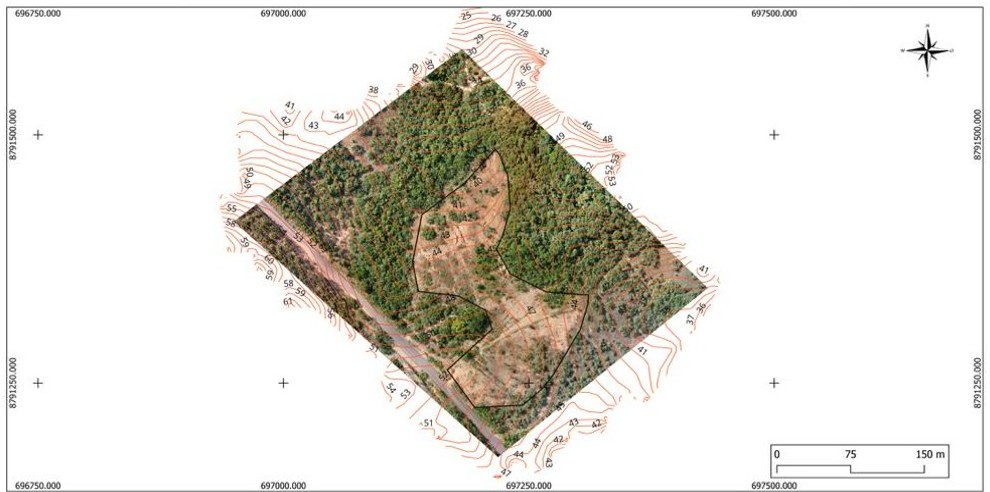
\includegraphics[width=0.8\linewidth,height=\textheight,keepaspectratio]{capitulos/../img/palicada_campo.jpg}

}

\caption{\label{fig-palicada-campo}Paliçada instalada em ravina ---
barreira transversal permeável que retarda o escoamento e promove a
deposição de sedimentos.}

\end{figure}%

\section{Materiais}\label{materiais}

A escolha do material para a paliçada depende da disponibilidade local,
do custo e da durabilidade necessária. Em regiões tropicais, três
materiais predominam.

\subsection{Bambu}\label{bambu}

O bambu (\emph{Bambusa} spp., \emph{Dendrocalamus} spp.) é o material
mais utilizado em regiões tropicais por combinar alta resistência à
tração (100--400 MPa, comparável a aço de construção), disponibilidade
abundante em propriedades rurais, baixo custo de aquisição, facilidade
de corte, transporte e montagem em campo (sem necessidade de ferramentas
especializadas) e durabilidade de 2--5 anos quando tratado com
preservativos naturais (imersão em solução de sulfato de cobre ou
tratamento por oclusão com bórax e ácido bórico). O bambu sem tratamento
degrada-se em 6--12 meses em ambiente tropical úmido, período que pode
ser suficiente para o estabelecimento vegetal em ravinas de pequeno
porte.

\subsection{Madeira Roliça}\label{madeira-roliuxe7a}

Troncos de eucalipto, pinus ou espécies nativas de rápido crescimento
(como leucena ou gliricídia) oferecem maior resistência mecânica e
durabilidade (3--8 anos sem tratamento, 10--15 anos com tratamento
autoclave). São indicados para ravinas de médio a grande porte onde a
pressão hidrostática exige maior robustez estrutural, mas seu custo e
peso são superiores ao bambu.

\subsection{Pedra Seca}\label{pedra-seca}

Em regiões com disponibilidade de pedras (encostas serranas, leitos
pedregosos de rios intermitentes), as paliçadas podem ser construídas
com pedras empilhadas sem argamassa, combinando função de filtro (a
permeabilidade entre as pedras permite a passagem da água enquanto retém
sedimentos grossos), alta durabilidade (décadas), resistência a
incêndios e nenhuma necessidade de manutenção. A desvantagem é o peso e
a dificuldade de transporte em terrenos íngremes.

\section{Dimensionamento}\label{dimensionamento}

O dimensionamento de paliçadas envolve três cálculos fundamentais que
determinam o espaçamento entre estruturas, a altura máxima e a
capacidade de retenção de sedimentos.

\subsection{Espaçamento entre
Paliçadas}\label{espauxe7amento-entre-paliuxe7adas}

O espaçamento (\(E\)) entre paliçadas consecutivas deve garantir que a
crista da paliçada a jusante esteja no mesmo nível que a base da
paliçada a montante, criando uma sequência de patamares que, quando
assoreados, eliminam o gradiente longitudinal original da ravina:

\[
E = \frac{H}{S_f}
\]

onde \(H\) é a altura efetiva da paliçada (porção acima do nível do
fundo da ravina, em metros) e \(S_f\) é a declividade do fundo da ravina
(em m/m, não em percentual). Por exemplo, para uma paliçada de 0,50 m de
altura efetiva em uma ravina com declividade de 10\% (0,10 m/m), o
espaçamento será de 5,0 m.

\subsection{Altura Efetiva}\label{altura-efetiva}

A altura efetiva da paliçada não deve exceder um terço da profundidade
da ravina na seção de instalação, garantindo que o escoamento possa
transbordar pela crista sem gerar erosão lateral:

\[
H_{max} = \frac{D}{3}
\]

onde \(D\) é a profundidade da ravina (m). Paliçadas mais altas que
\(D/3\) geram represamento excessivo, com risco de erosão por contorno
(a água contorna a estrutura pelas laterais, escavando as paredes da
ravina) ou de ruptura por sobrecarga hidrostática.

\subsection{Capacidade de Retenção}\label{capacidade-de-retenuxe7uxe3o}

O volume de sedimento retido por uma paliçada pode ser estimado pela
geometria do prisma trapezoidal que se forma a montante da estrutura:

\[
V_r = \frac{E \cdot W \cdot H}{2}
\]

onde \(W\) é a largura da ravina na posição da paliçada. Esse volume
permite estimar o tempo de preenchimento e, consequentemente, a
necessidade de manutenção ou substituição.

\section{Construção}\label{construuxe7uxe3o}

O processo de construção de uma paliçada de bambu é relativamente
simples e pode ser executado por equipes de 2--4 trabalhadores com
ferramentas manuais (enxada, facão, marreta). A
Figura~\ref{fig-instalacao} ilustra as etapas de instalação em
sequência.

\begin{figure}

\centering{

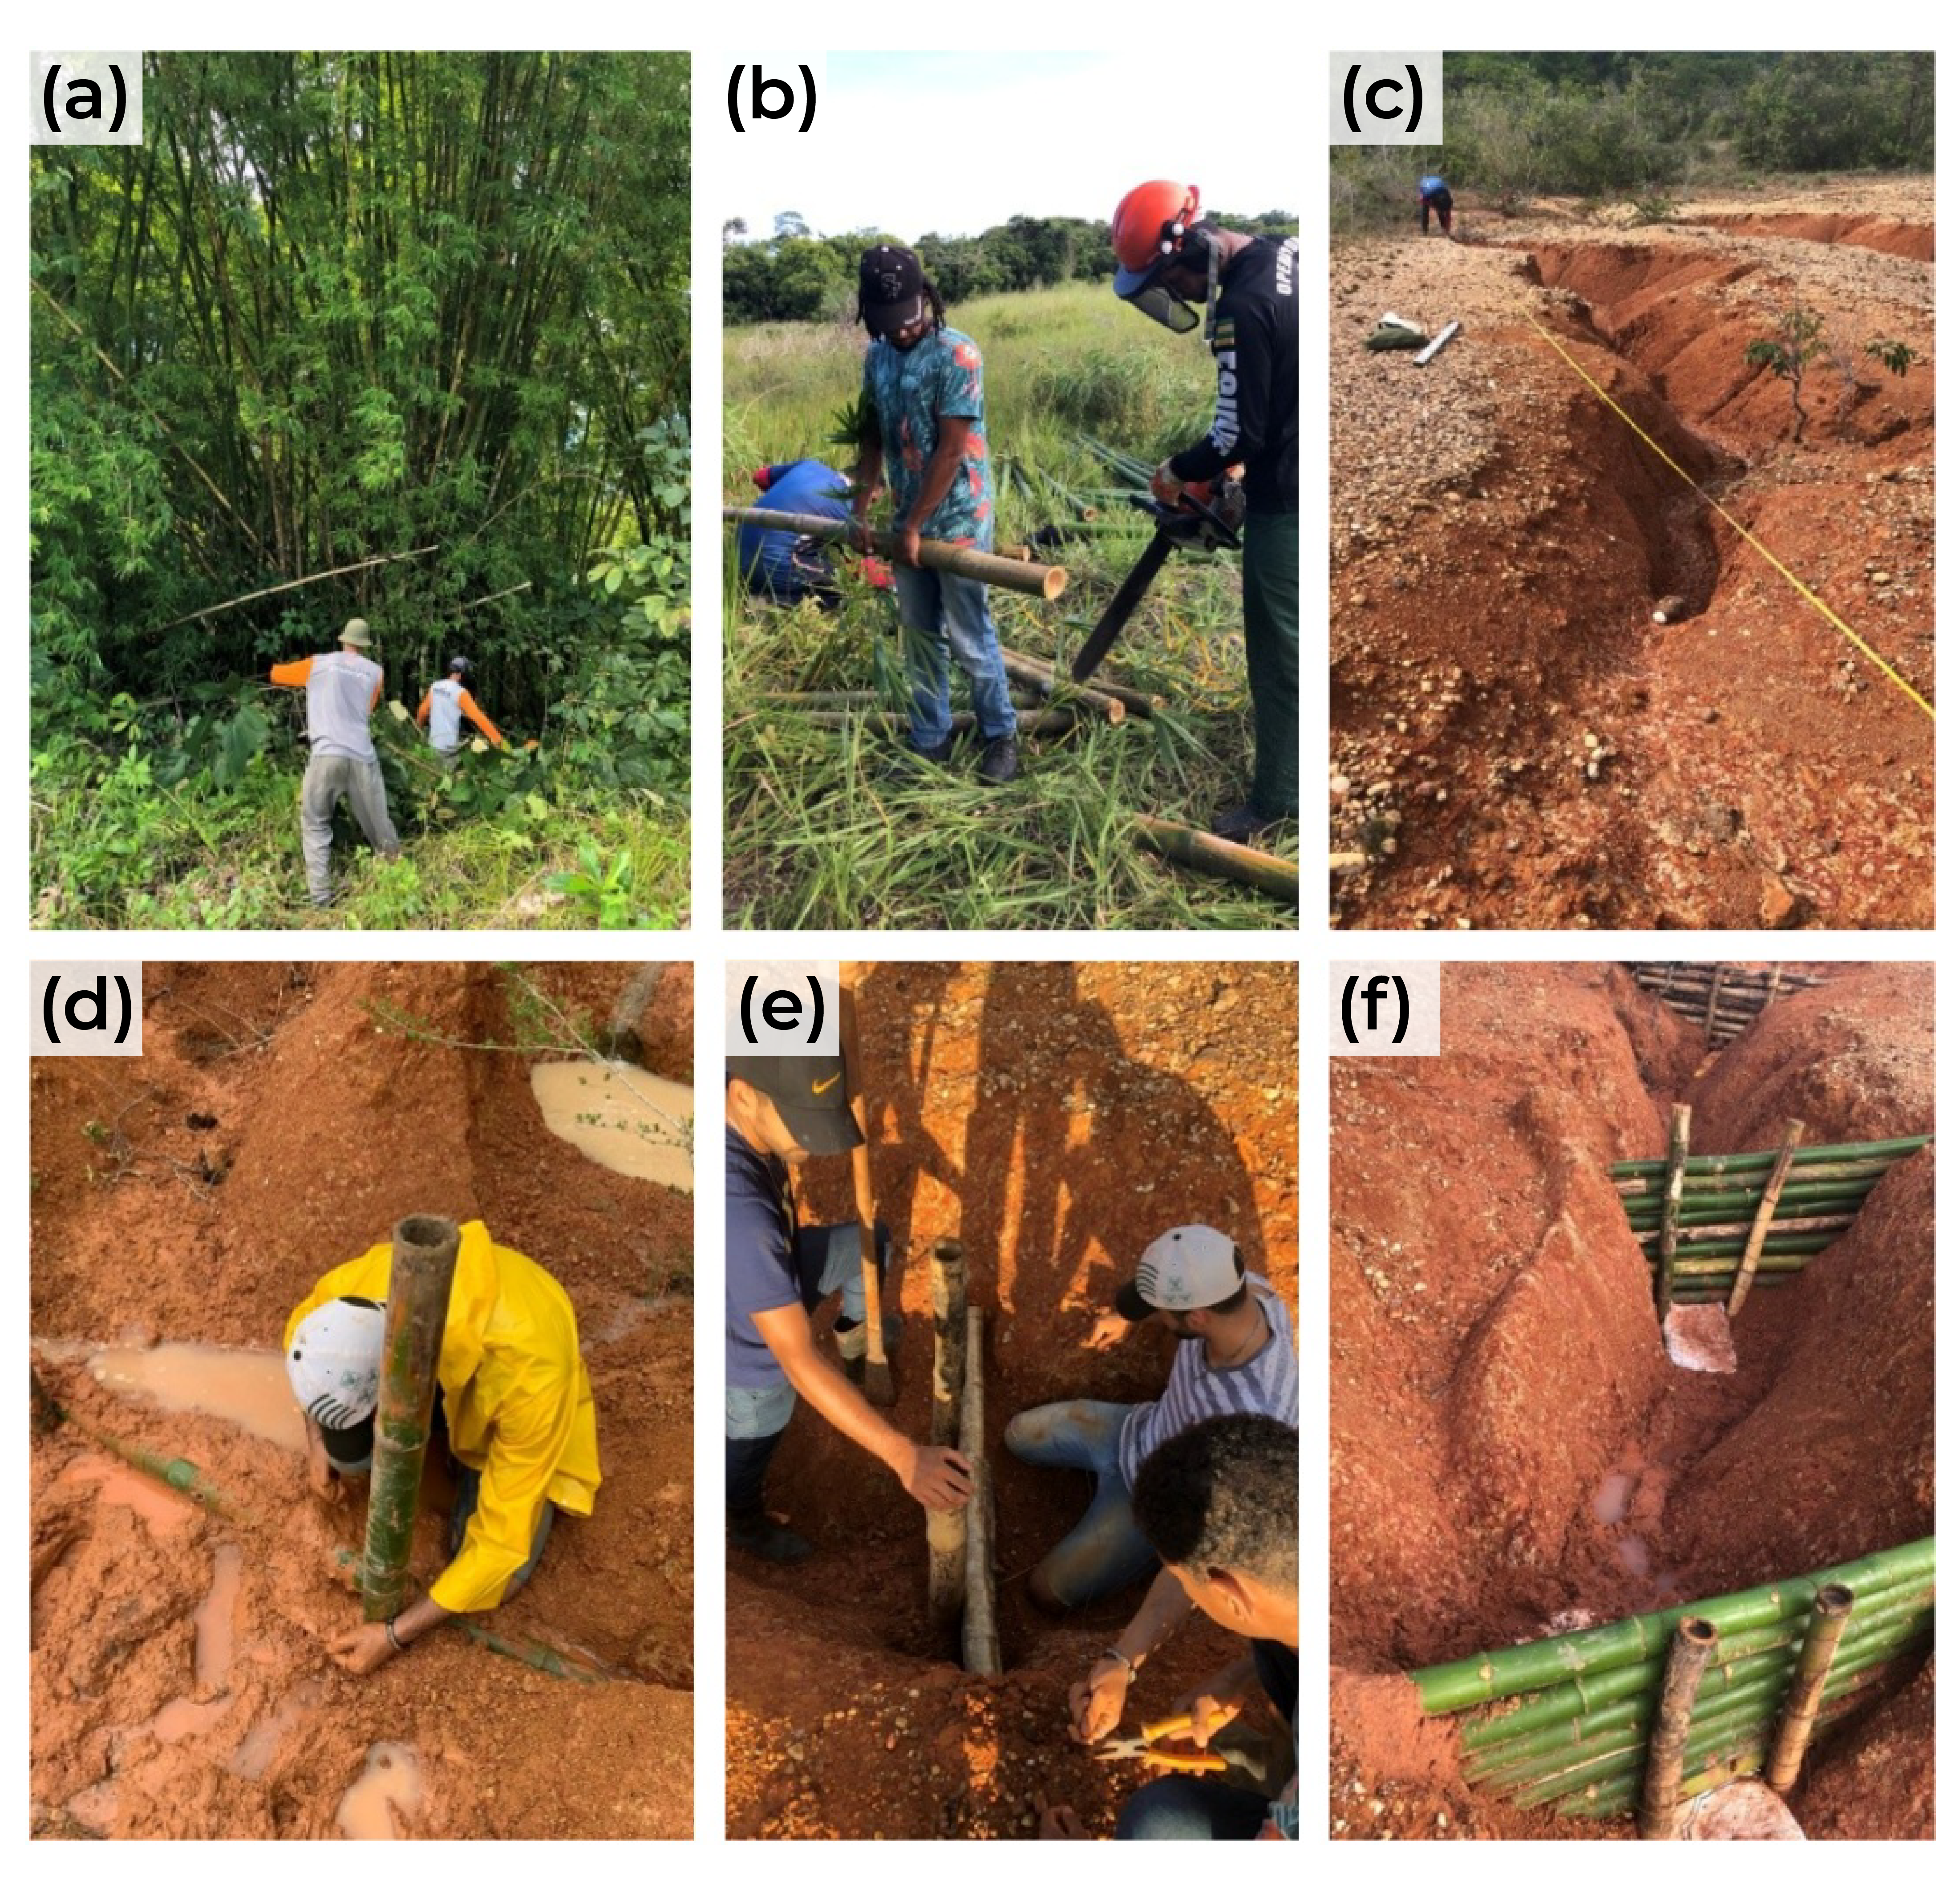
\includegraphics[width=0.85\linewidth,height=\textheight,keepaspectratio]{capitulos/../img/instalacao_palicadas.png}

}

\caption{\label{fig-instalacao}Etapas de instalação de paliçadas em
ravina --- escavação, cravamento de estacas e entrelaçamento das varas.}

\end{figure}%

\subsection{Passo a Passo}\label{passo-a-passo}

Conforme mostrado na Figura~\ref{fig-instalacao}, o procedimento inicia
com a escavação de uma vala transversal perpendicular ao eixo da ravina,
com profundidade igual à altura efetiva \(H\) (ou seja, metade da
paliçada ficará enterrada, garantindo ancoragem contra tombamento e
percolação por baixo). Em seguida, realiza-se o cravamento de estacas
verticais de bambu ou madeira a cada 30--50 cm ao longo da vala, com
cada estaca penetrando ao menos 30 cm abaixo do fundo da vala. O
entrelaçamento de varas horizontais entre as estacas é feito alternando
os lados (frente e trás), de forma análoga à tecelagem, criando uma
estrutura flexível mas resistente. Após o entrelaçamento, compacta-se
terra contra a face montante da paliçada para vedar a base e evitar
percolação concentrada. As laterais são ancoradas nas paredes da ravina
por pelo menos 50 cm de cada lado, com as varas horizontais embutidas em
entalhes escavados nas paredes. Por fim, semeiam-se gramíneas a montante
da paliçada para acelerar a cobertura vegetal sobre os sedimentos que
serão depositados.

\begin{tcolorbox}[enhanced jigsaw, leftrule=.75mm, colframe=quarto-callout-important-color-frame, colback=white, bottomrule=.15mm, opacityback=0, colbacktitle=quarto-callout-important-color!10!white, breakable, bottomtitle=1mm, opacitybacktitle=0.6, title=\textcolor{quarto-callout-important-color}{\faExclamation}\hspace{0.5em}{Ponto crítico}, titlerule=0mm, toprule=.15mm, toptitle=1mm, rightrule=.15mm, left=2mm, arc=.35mm, coltitle=black]

As paliçadas devem ser ancoradas nas paredes laterais da ravina por pelo
menos 50 cm de cada lado. A principal causa de falha em paliçadas é a
erosão lateral por contorno da estrutura, que ocorre quando a água
encontra caminho mais fácil pelas laterais do que pelo corpo permeável
da paliçada. A ancoragem insuficiente é um erro de projeto que
compromete toda a intervenção.

\end{tcolorbox}

\section{Eficiência}\label{eficiuxeancia}

Os dados de eficiência das paliçadas são essenciais para justificar
tecnicamente a escolha dessa técnica em detrimento de alternativas mais
caras. A Figura~\ref{fig-simulacao} apresenta a evolução temporal da
retenção de sedimentos em uma sequência de paliçadas, demonstrando como
o assoreamento progressivo cria patamares que estabilizam o perfil
longitudinal da ravina.

\begin{figure}

\centering{

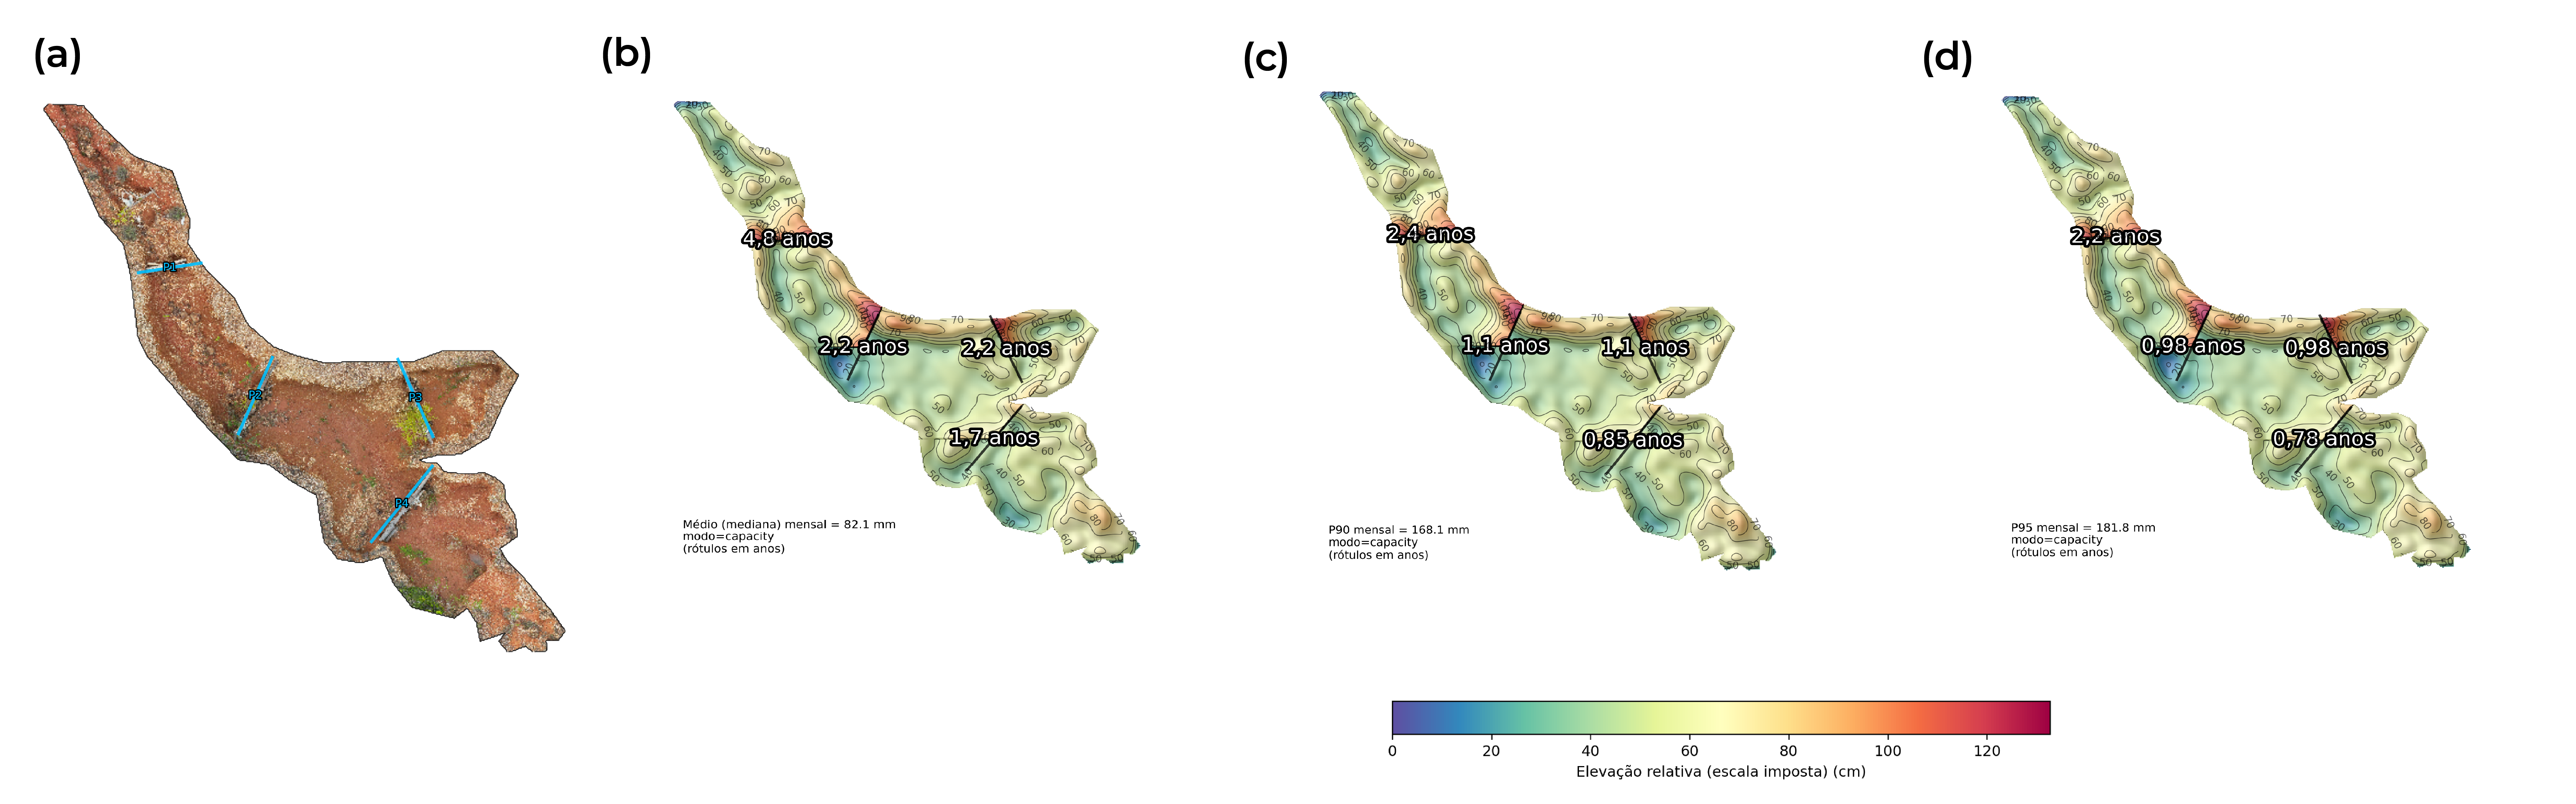
\includegraphics[width=0.85\linewidth,height=\textheight,keepaspectratio]{capitulos/../img/simulacao_palicadas.png}

}

\caption{\label{fig-simulacao}Simulação temporal de retenção de
sedimentos pelas paliçadas ao longo dos anos --- o assoreamento
progressivo cria patamares que estabilizam a ravina.}

\end{figure}%

\begin{figure}

\centering{

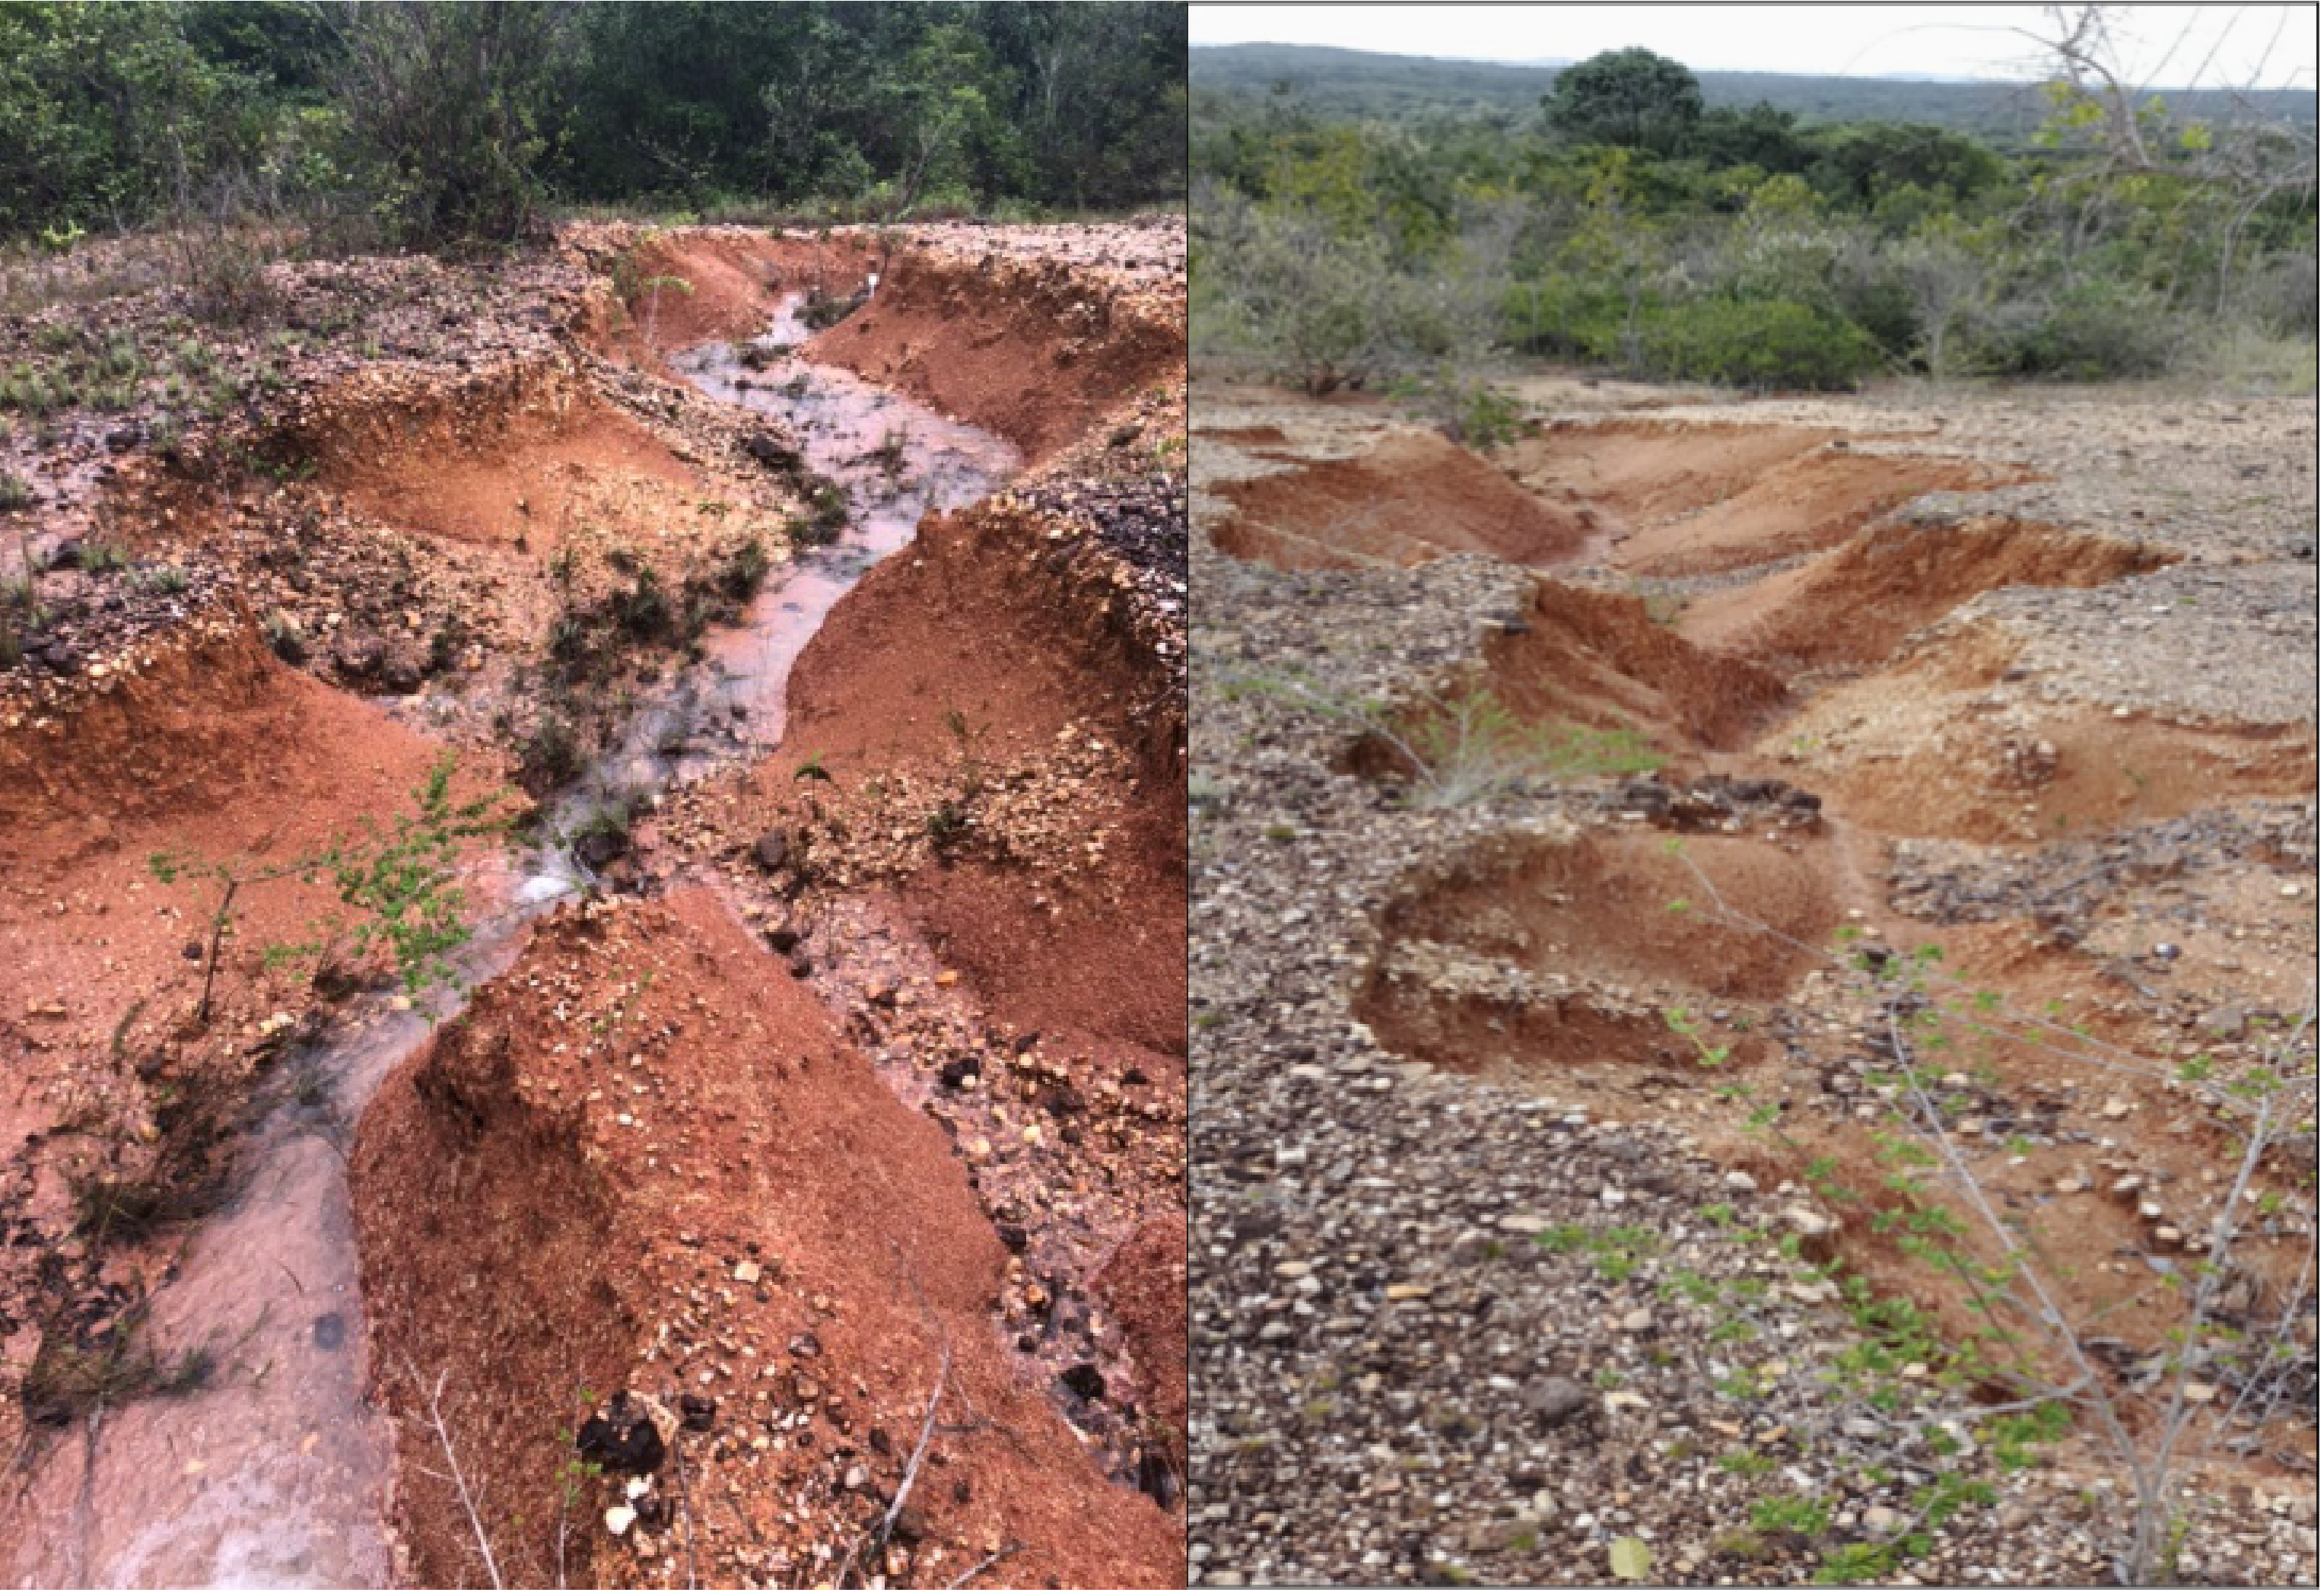
\includegraphics[width=0.8\linewidth,height=\textheight,keepaspectratio]{capitulos/../img/area_estudo_palicadas.png}

}

\caption{\label{fig-area-estudo-palicadas}Área de estudo --- localização
das paliçadas experimentais em ravinas nos Tabuleiros Costeiros de
Sergipe.}

\end{figure}%

Conforme observado na Figura~\ref{fig-simulacao}, o processo de
estabilização é progressivo. Estudos em Plintossolo degradado nos
Tabuleiros Costeiros de Sergipe demonstraram resultados quantitativos
expressivos: retenção de 76 cm de sedimento em 12 meses (paliçada de 1,0
m de altura), redução de 85\% na velocidade do escoamento no interior da
ravina e colonização vegetal espontânea a montante das paliçadas após 6
meses. A projeção de preenchimento total do espaço entre paliçadas
consecutivas estima-se entre 3 e 5 anos, período no qual a vegetação
assume progressivamente a função de estabilização, realizando a
transição funcional discutida no \textbf{?@sec-introducao}.

\section{Custos Comparativos}\label{custos-comparativos}

A viabilidade econômica das paliçadas de bambu em relação às
alternativas convencionais (check-dams de alvenaria ou concreto) é uma
das principais vantagens da técnica, conforme demonstrado na
Tabela~\ref{tbl-custos-palicada}.

\begin{longtable}[]{@{}lll@{}}
\caption{Comparativo de custos entre paliçadas de bambu e check-dams de
alvenaria.}\label{tbl-custos-palicada}\tabularnewline
\toprule\noalign{}
Item & Paliçada de bambu & Check-dam de alvenaria \\
\midrule\noalign{}
\endfirsthead
\toprule\noalign{}
Item & Paliçada de bambu & Check-dam de alvenaria \\
\midrule\noalign{}
\endhead
\bottomrule\noalign{}
\endlastfoot
Material & R\$ 15--30/m² & R\$ 150--300/m² \\
Mão de obra & R\$ 20--40/m² & R\$ 80--150/m² \\
Total & R\$ 35--70/m² & R\$ 230--450/m² \\
Vida útil & 3--5 anos & 20+ anos \\
Manutenção & Anual & Quinquenal \\
\end{longtable}

\begin{tcolorbox}[enhanced jigsaw, leftrule=.75mm, colframe=quarto-callout-tip-color-frame, colback=white, bottomrule=.15mm, opacityback=0, colbacktitle=quarto-callout-tip-color!10!white, breakable, bottomtitle=1mm, opacitybacktitle=0.6, title=\textcolor{quarto-callout-tip-color}{\faLightbulb}\hspace{0.5em}{Vantagem econômica}, titlerule=0mm, toprule=.15mm, toptitle=1mm, rightrule=.15mm, left=2mm, arc=.35mm, coltitle=black]

O custo das paliçadas de bambu é 5 a 7× menor que check-dams de
alvenaria. Mesmo considerando a reposição a cada 5 anos (três ciclos em
15 anos), o custo acumulado das paliçadas permanece inferior ao da
solução convencional. Adicionalmente, as paliçadas podem ser construídas
com mão de obra local não especializada, o que gera renda na comunidade
e reduz custos logísticos de transporte de materiais pesados (cimento,
areia, brita).

\end{tcolorbox}

\chapter{Bacias de Captação}\label{bacias-de-captauxe7uxe3o}

\# Bacias de Captação e Barraginhas \{\#sec-bacias-captacao\}

As bacias de captação (ou barraginhas) são estruturas de retenção de
enxurrada escavadas ao longo de estradas rurais ou em encostas, cujo
propósito é interceptar, reter e infiltrar o escoamento superficial
antes que ele cause erosão a jusante. Em essência, trata-se de pequenas
depressões côncavas escavadas no solo (normalmente com formato de
meia-lua ou circular), dimensionadas para receber o volume de enxurrada
gerado pela área de contribuição a montante. A água captada permanece na
bacia por horas a dias, infiltrando gradualmente no solo e recarregando
o lençol freático, em vez de escoar em alta velocidade pela superfície,
erodindo estradas e formando ravinas.

A técnica foi amplamente difundida pela Embrapa Milho e Sorgo no
Semiárido brasileiro, onde estradas rurais não pavimentadas concentram o
escoamento superficial e geram ravinas laterais que, sem intervenção,
evoluem para voçorocas em poucos anos. No entanto, a aplicabilidade das
barraginhas estende-se a qualquer região onde o escoamento superficial
concentrado cause erosão em estradas, encostas ou áreas de pastagem
degradada. A Figura~\ref{fig-barraginha} mostra uma barraginha típica
implantada em estrada rural, onde se observa a geometria côncava da
escavação e a interceptação do escoamento lateral.

\begin{figure}

\centering{

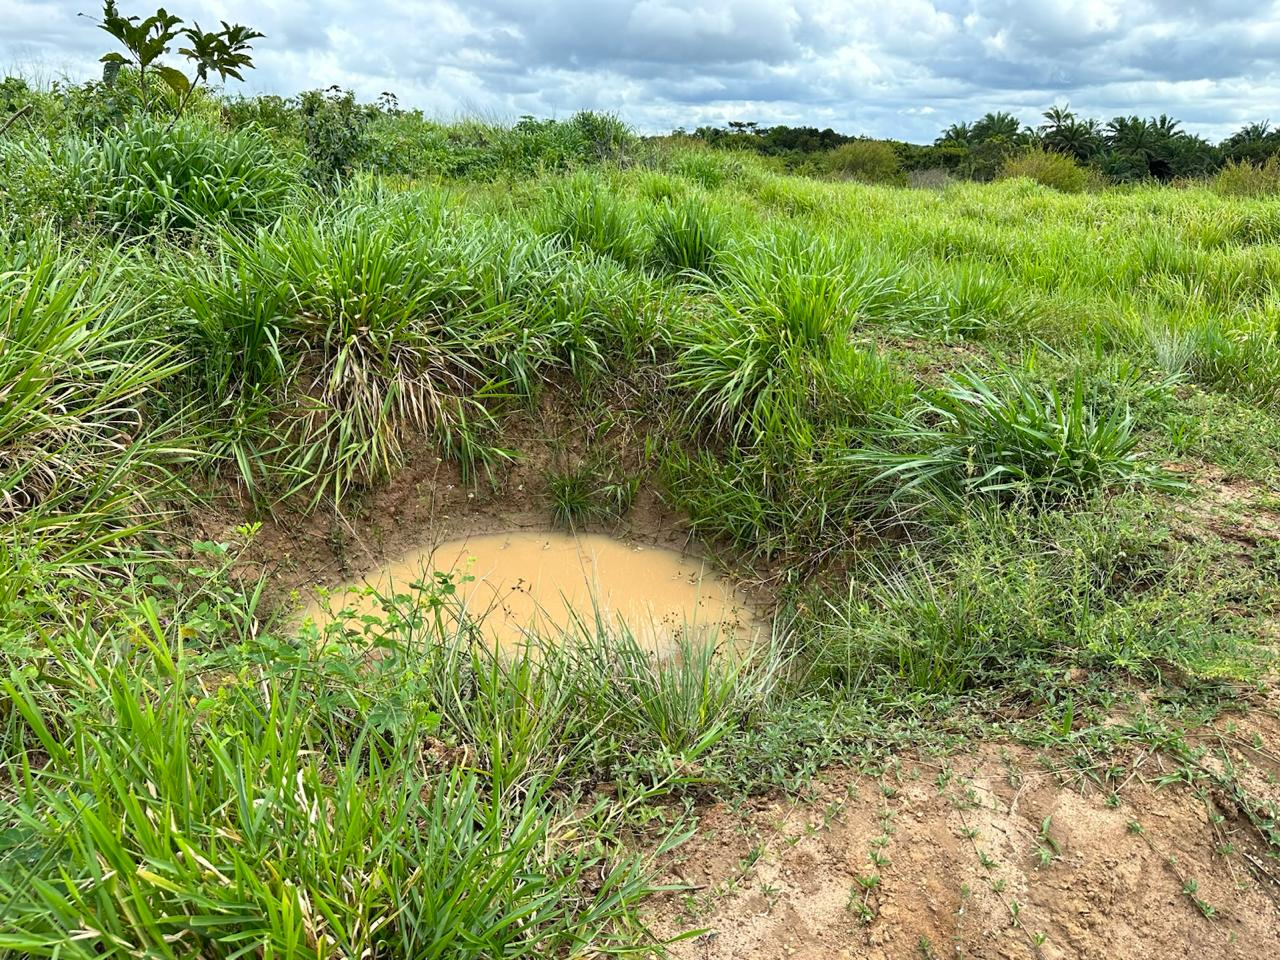
\includegraphics[width=0.8\linewidth,height=\textheight,keepaspectratio]{capitulos/../img/barraginha_1.jpeg}

}

\caption{\label{fig-barraginha}Barraginha implantada em estrada rural
--- estrutura de retenção que intercepta e infiltra o escoamento
superficial.}

\end{figure}%

\section{Funções}\label{funuxe7uxf5es}

As bacias de captação desempenham quatro funções hidrológicas e
geomorfológicas interconectadas. A retenção de sedimentos é a função
mais imediata, operando com eficiência de 50--80\% na remoção de
partículas do escoamento, uma vez que a redução brusca de velocidade da
água ao entrar na bacia causa a deposição gravitacional das partículas
em suspensão: primeiro as areias (em minutos), depois os siltes (em
horas) e por último as argilas floculadas (em dias). A recarga de
aquíferos é a função menos visível mas mais relevante para a
sustentabilidade hídrica da paisagem, promovendo infiltração de 20--60
m³ por evento chuvoso, o que equivale, em uma propriedade com 30
barraginhas, a um volume anual de recarga da ordem de 2.000--6.000 m³. O
amortecimento do pico de cheia pode atingir 40\% de redução na vazão
máxima a jusante, protegendo pontes, bueiros e estradas de acessso. A
proteção de estradas rurais evita a formação de ravinas laterais ao
interceptar o escoamento antes que ele atinja velocidades erosivas.

A Figura~\ref{fig-barraginha2} permite observar o funcionamento
hidráulico da bacia após um evento chuvoso, com a água retida
infiltrando gradualmente no solo, enquanto a
Figura~\ref{fig-mapa-decliv} demonstra como o planejamento espacial das
barraginhas é orientado por critérios topográficos, com a declividade do
terreno determinando o espaçamento e o posicionamento ideal das
estruturas.

\begin{figure}

\begin{minipage}{0.50\linewidth}

\begin{figure}[H]

\centering{

\pandocbounded{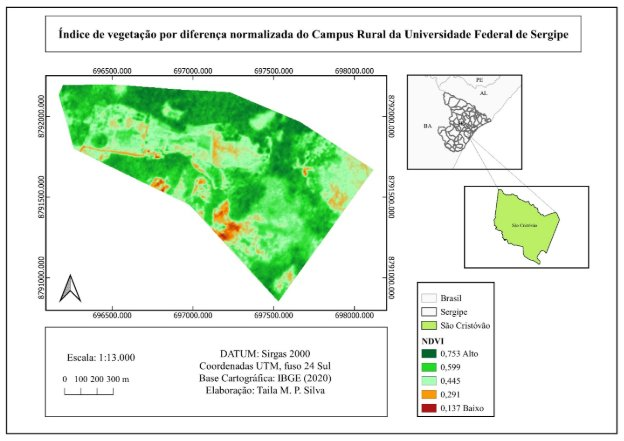
\includegraphics[keepaspectratio]{capitulos/../img/barraginha_2.jpg}}

}

\caption{\label{fig-barraginha2}Detalhe de barraginha após chuva --- a
água é retida e infiltra gradualmente no solo.}

\end{figure}%

\end{minipage}%
%
\begin{minipage}{0.50\linewidth}

\begin{figure}[H]

\centering{

\pandocbounded{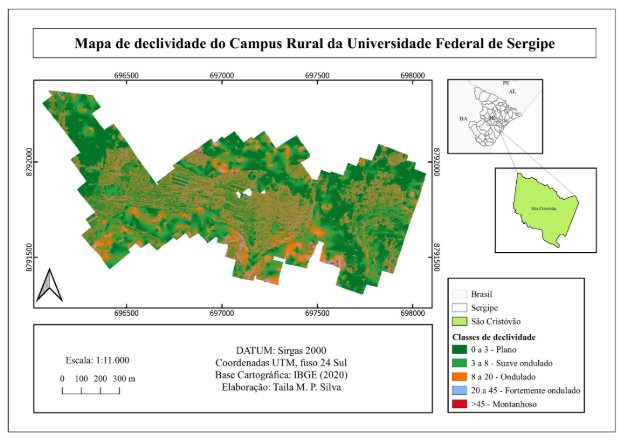
\includegraphics[keepaspectratio]{capitulos/../img/mapa_declividade.jpg}}

}

\caption{\label{fig-mapa-decliv}Mapa de declividade para planejamento de
barraginhas --- a localização é definida por critérios topográficos.}

\end{figure}%

\end{minipage}%

\end{figure}%

\section{Dimensionamento}\label{dimensionamento-1}

O dimensionamento adequado é o fator determinante da eficiência das
barraginhas. Uma bacia subdimensionada transbordará com frequência,
anulando suas funções de retenção e infiltração; uma bacia
superdimensionada representa desperdício de recursos de escavação e
ocupa área útil desnecessariamente. O dimensionamento envolve três
cálculos fundamentais.

\subsection{Método EUPS + VIB}\label{muxe9todo-eups-vib}

O volume da bacia deve ser suficiente para conter o escoamento gerado
por uma chuva de projeto (tipicamente com período de retorno de 10 anos
e duração igual ao tempo de concentração da área de contribuição),
descontando-se a parcela que infiltra durante o próprio evento. A
equação que integra esses fatores é

\[
V_{bacia} = A_c \cdot P \cdot C \cdot (1 - VIB/P)
\]

onde \(A_c\) é a área de contribuição (m²), que corresponde à porção do
terreno cujo escoamento é direcionado para a bacia pelo relevo e pela
infraestrutura viária; \(P\) é a precipitação de projeto (m), obtida a
partir de curvas IDF (Intensidade-Duração-Frequência) da estação
meteorológica mais próxima; \(C\) é o coeficiente de escoamento
superficial (adimensional, tipicamente 0,30--0,60 para estradas não
pavimentadas e 0,10--0,30 para pastagens); e \(VIB\) é a velocidade de
infiltração básica do solo (m/h), determinada por ensaio de infiltração
com infiltrômetro de duplo anel conforme a norma ABNT NBR 7229. O termo
\((1 - VIB/P)\) representa a fração da chuva que efetivamente gera
escoamento, descontada a infiltração simultânea.

\begin{figure}

\centering{

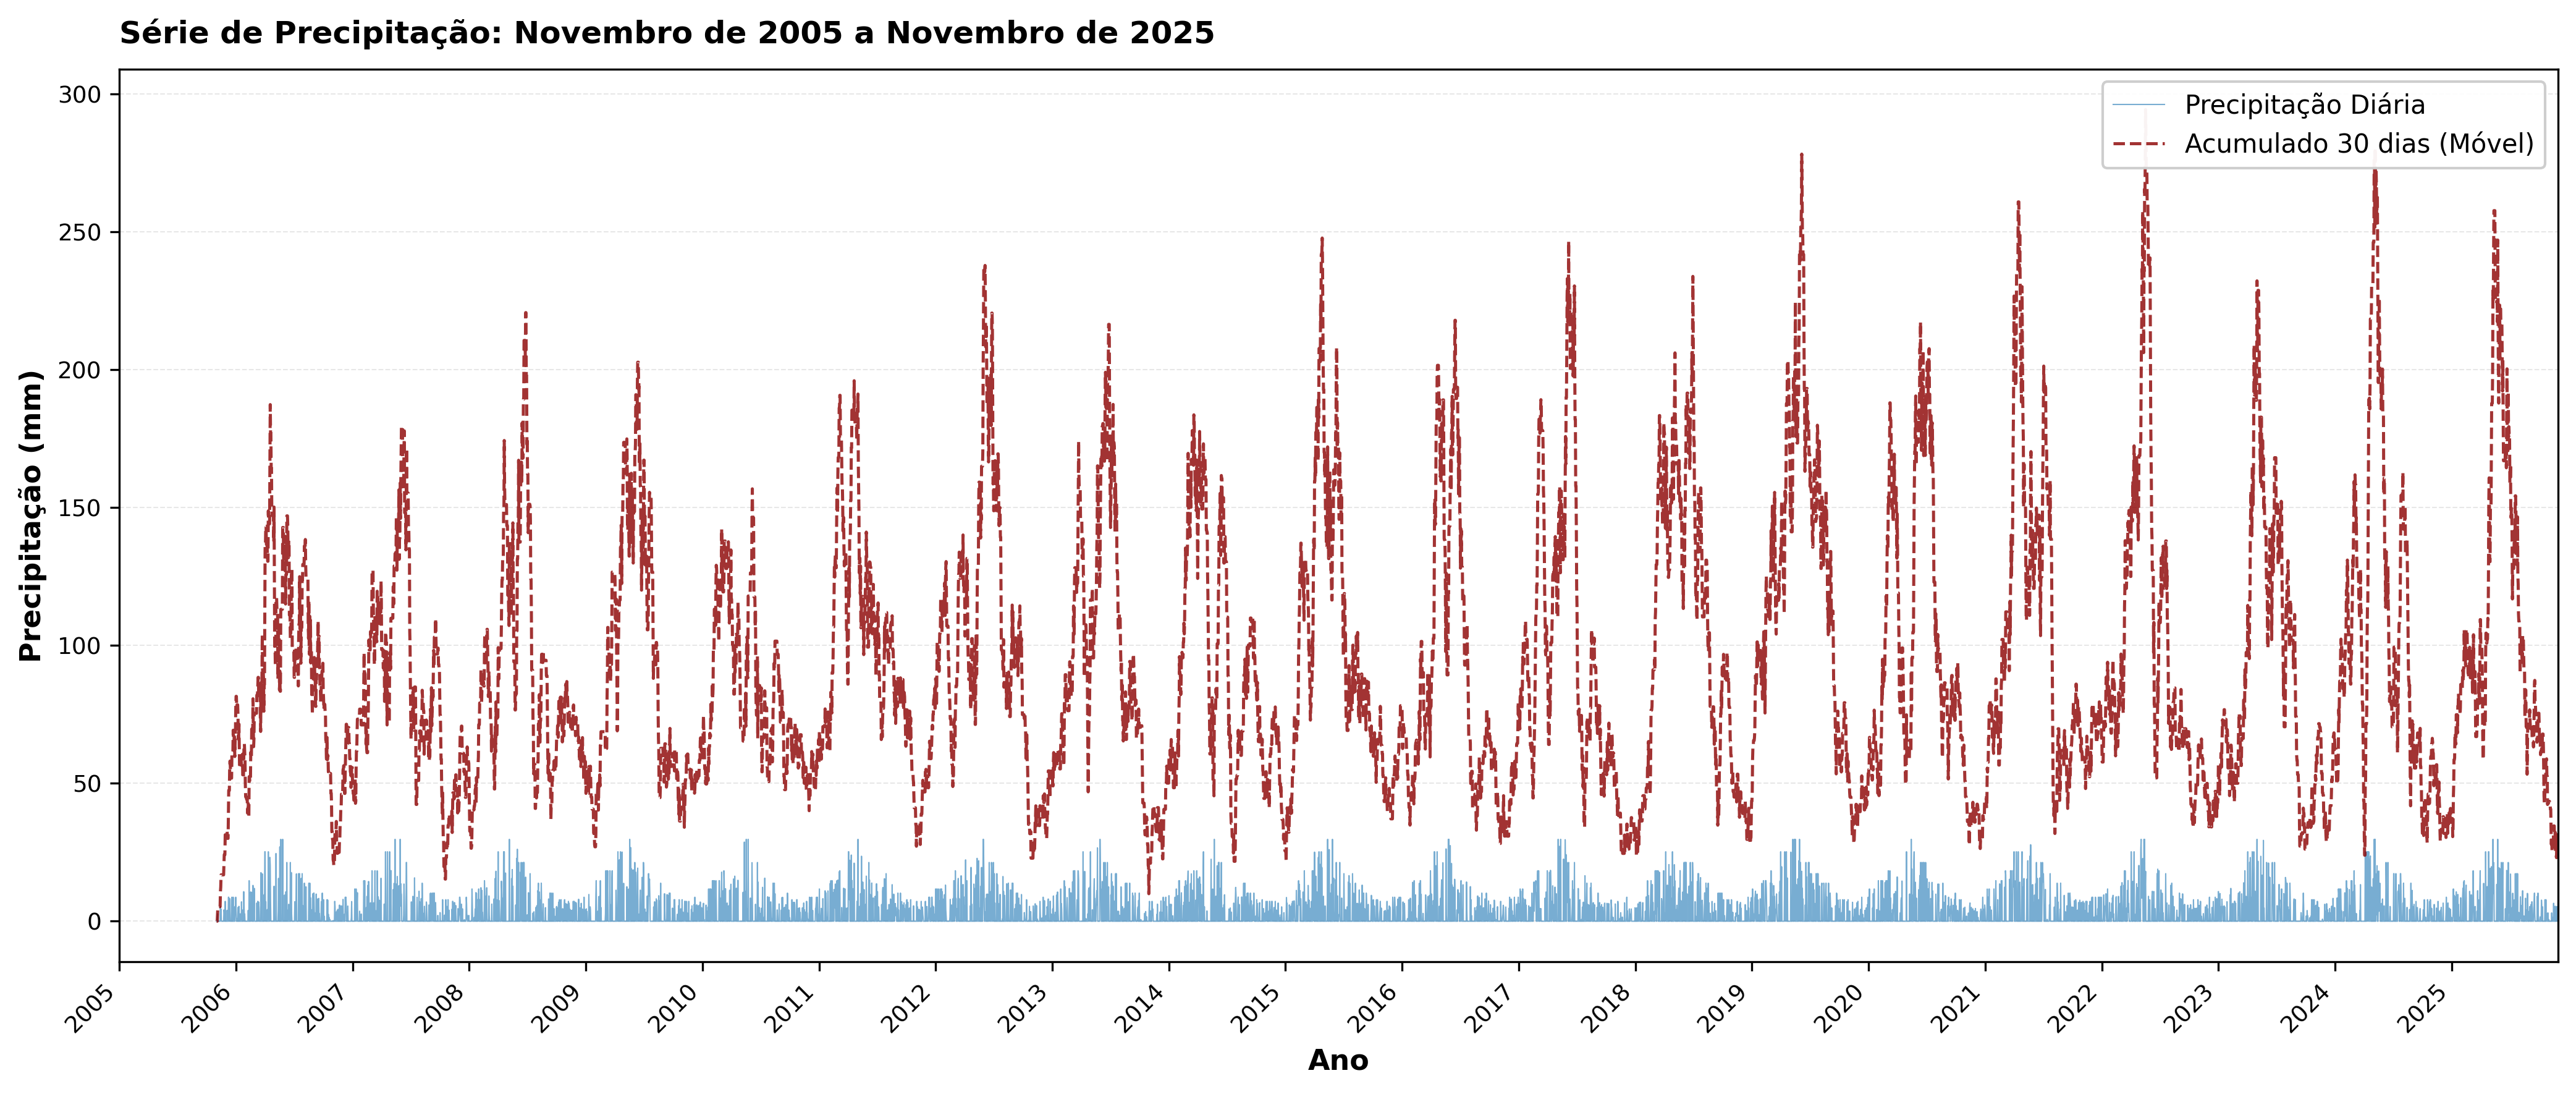
\includegraphics[width=0.8\linewidth,height=\textheight,keepaspectratio]{capitulos/../img/precipitacao.png}

}

\caption{\label{fig-precipitacao}Distribuição da precipitação --- série
pluviométrica e curvas IDF utilizadas para determinação da precipitação
de projeto (\(P\)) no dimensionamento de bacias de captação.}

\end{figure}%

\subsection{Área de Contribuição}\label{uxe1rea-de-contribuiuxe7uxe3o}

Para estradas rurais, a área de contribuição é calculada como

\[
A_c = L \cdot (W_{estrada} + W_{talude})
\]

onde \(L\) é o comprimento da estrada que drena para a bacia (m),
\(W_{estrada}\) é a largura da plataforma da estrada (tipicamente 4--8 m
para estradas vicinais) e \(W_{talude}\) é a largura horizontal do
talude de corte a montante que também contribui com escoamento para a
estrada (0--5 m, dependendo da geometria). A identificação precisa de
\(A_c\) pode ser realizada em campo com nível de mangueira ou, de forma
mais acurada, a partir de Modelo Digital de Terreno (MDT) com resolução
mínima de 1 m, conforme abordagem discutida na
Figura~\ref{fig-mapa-decliv}.

\subsection{Dimensões Típicas}\label{dimensuxf5es-tuxedpicas}

A Tabela~\ref{tbl-dimensoes-bacia} sintetiza os valores típicos de
dimensionamento adotados em projetos de barraginhas para estradas rurais
no Brasil.

\begin{longtable}[]{@{}lll@{}}
\caption{Dimensões típicas de bacias de captação para estradas
rurais.}\label{tbl-dimensoes-bacia}\tabularnewline
\toprule\noalign{}
Parâmetro & Valor típico & Observação \\
\midrule\noalign{}
\endfirsthead
\toprule\noalign{}
Parâmetro & Valor típico & Observação \\
\midrule\noalign{}
\endhead
\bottomrule\noalign{}
\endlastfoot
Profundidade & 0,8--1,5 m & Limitada pelo nível do lençol freático \\
Diâmetro superior & 3--6 m & Maior em solos com baixa VIB \\
Volume & 5--30 m³ & Proporcional a \(A_c\) \\
Espaçamento & 30--80 m & Reduzir em declividades \textgreater{} 8\% \\
Declividade lateral & 1:1 a 1:1,5 & Mais suave em solos arenosos \\
\end{longtable}

\section{Espaçamento}\label{espauxe7amento}

O espaçamento entre bacias consecutivas deve garantir que cada uma
receba um volume compatível com sua capacidade, sem que o escoamento
excedente gere erosão no trecho entre bacias sucessivas. A equação de
espaçamento é

\[
E_{bacias} = \frac{V_{bacia}}{W_{estrada} \cdot P \cdot C}
\]

Em terrenos com declividade \textgreater{} 8\%, o espaçamento deve ser
reduzido em 30--50\%, pois a velocidade do escoamento aumenta e o tempo
de concentração diminui, gerando picos de vazão mais intensos que exigem
maior capacidade de retenção por unidade de comprimento de estrada. Uma
regra prática amplamente adotada em programas de conservação de estradas
rurais é posicionar as barraginhas nos pontos naturais de concentração
de enxurrada (curvas, depressões, confluências de trilhas laterais),
ajustando o espaçamento calculado à realidade topográfica do terreno.

\section{Vida Útil e Manutenção}\label{vida-uxfatil-e-manutenuxe7uxe3o}

A vida útil projetada das bacias situa-se entre 10 e 20 anos, dependendo
fundamentalmente da taxa de produção de sedimentos na área de
contribuição a montante (que por sua vez depende do tipo de solo,
cobertura vegetal, uso da terra e declividade) e da frequência de
manutenção. O assoreamento é o principal fator de degradação das
barraginhas, reduzindo progressivamente o volume útil disponível para
retenção de enxurrada. O monitoramento deve acompanhar a evolução do
nível de sedimentos no interior da bacia, e a manutenção principal
consiste na limpeza mecanizada (retroescavadeira) a cada 2--5 anos,
removendo o sedimento acumulado e restaurando a capacidade de retenção
original. O sinal de esgotamento funcional é o assoreamento superior a
70\% da capacidade, quando a bacia já não consegue amortecer
adequadamente os picos de cheia e passa a transbordar com frequência.

O sedimento removido das bacias pode ser reaproveitado como material de
aterro em estradas ou como substrato para revegetação de áreas
degradadas, fechando o ciclo de materiais e reduzindo custos de
disposição.

\begin{tcolorbox}[enhanced jigsaw, leftrule=.75mm, colframe=quarto-callout-warning-color-frame, colback=white, bottomrule=.15mm, opacityback=0, colbacktitle=quarto-callout-warning-color!10!white, breakable, bottomtitle=1mm, opacitybacktitle=0.6, title=\textcolor{quarto-callout-warning-color}{\faExclamationTriangle}\hspace{0.5em}{Atenção}, titlerule=0mm, toprule=.15mm, toptitle=1mm, rightrule=.15mm, left=2mm, arc=.35mm, coltitle=black]

Em solos com VIB muito baixa (\textless{} 5 mm/h), como Vertissolos ou
Planossolos, as bacias podem transbordar com frequência mesmo quando
adequadamente dimensionadas. Nesses casos, o projetista deve dimensionar
com chuva de menor período de retorno (5 anos) ou prever um sangradouro
lateral vegetado, que é um canal de extravasamento revestido com
gramíneas (preferencialmente \emph{Paspalum notatum} ou \emph{Cynodon}
spp.) que conduz o excedente para a bacia seguinte sem causar erosão.

\end{tcolorbox}

\section{Custos}\label{custos}

Os custos de implantação variam entre R\$ 200 e R\$ 500 por bacia para
escavação mecanizada com retroescavadeira (1--2 horas de máquina por
bacia, incluindo mobilização e desmobilização) e entre R\$ 400 e R\$ 800
por bacia para escavação manual (2--3 dias de trabalho de 2 operários,
indicada para locais sem acesso para máquinas). O custo por hectare
protegido situa-se entre R\$ 500 e R\$ 1.500, considerando a densidade
média de 3--5 bacias/ha em estradas rurais com declividade moderada.

A relação custo-benefício é extremamente favorável, com evidências de
que cada real investido em barraginhas evita R\$ 5--12 em custos de
manutenção de estradas rurais (patrolamento, reposição de cascalho,
reconstrução de bueiros danificados), além dos benefícios indiretos de
recarga hídrica, redução de assoreamento de corpos d'água a jusante e
preservação de áreas de cultivo adjacentes.

\chapter{\texorpdfstring{Feixes Vivos
(\emph{Fascines})}{Feixes Vivos (Fascines)}}\label{feixes-vivos-fascines}

\# Feixes Vivos e Drenos Verdes \{\#sec-feixes-drenos\}

\subsection{Feixes Vivos}\label{feixes-vivos}

Os feixes vivos (\emph{fascines} ou \emph{wattle fences}) são amarrados
de ramos vivos e flexíveis, dispostos em valas rasas ao longo de curvas
de nível para interceptar o escoamento superficial laminar e promover
simultaneamente a infiltração e a retenção de sedimentos. O princípio de
funcionamento é análogo ao das paliçadas (ver \textbf{?@sec-palicadas}),
porém os feixes atuam contra o escoamento difuso em encostas (não
concentrado em ravinas), funcionando como barreiras lineares de baixa
altura (15--30 cm) que fragmentam a lâmina d'água, reduzem a velocidade
superficial e criam uma zona de deposição a montante onde sedimentos
finos se acumulam e a vegetação se restabelece.

A grande vantagem dos feixes em relação a cordões de pedra ou leiras de
terra é que, sendo compostos por ramos vivos, enraízam e brotam após a
instalação, transformando-se progressivamente em sebes vivas que mantêm
e até ampliam sua função de barreira ao longo do tempo, sem necessidade
de reposição. Essa transição de estrutura morta para estrutura viva é o
mecanismo central que confere sustentabilidade à técnica. A
Figura~\ref{fig-feixes-campo} mostra feixes vivos recém-instalados em
campo, onde se observam os amarrados de ramos posicionados em valas
rasas e fixados com estacas verticais.

\begin{figure}

\centering{

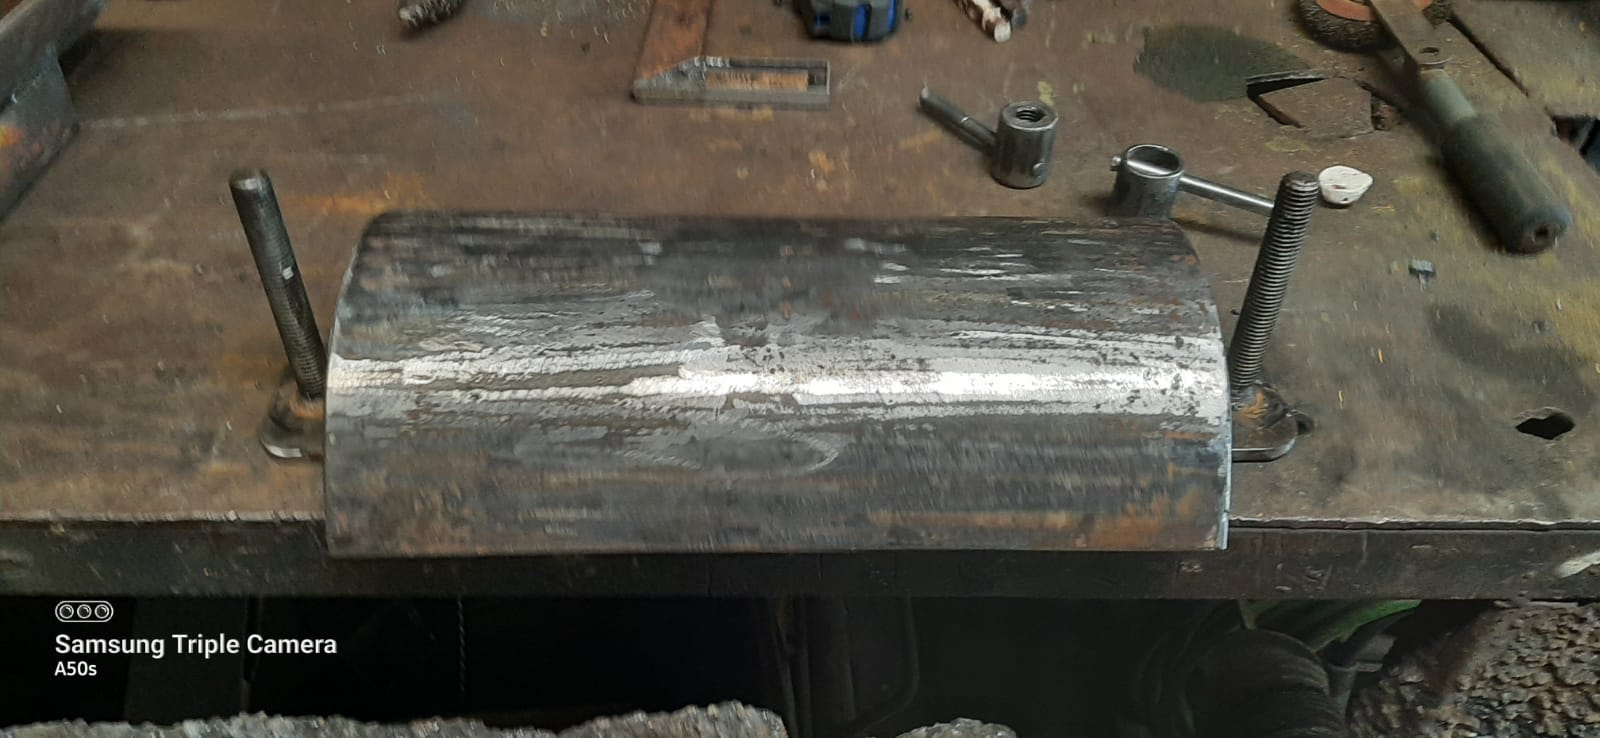
\includegraphics[width=0.8\linewidth,height=\textheight,keepaspectratio]{capitulos/../img/feixes_vivos_campo.jpg}

}

\caption{\label{fig-feixes-campo}Feixes vivos em campo --- amarrados de
ramos vivos instalados em valas para interceptar o escoamento e promover
a infiltração.}

\end{figure}%

A Figura~\ref{fig-feixe-diagrama} apresenta o diagrama em corte
transversal do feixe instalado na vala, detalhando as proporções entre
profundidade de enterramento, diâmetro do feixe e altura exposta acima
da superfície. Já a Figura~\ref{fig-estacas} mostra em detalhe o
material vegetativo utilizado como estacas de fixação, evidenciando os
pontos de brotação que garantem o enraizamento futuro da estrutura.

\begin{figure}

\begin{minipage}{0.50\linewidth}

\begin{figure}[H]

\centering{

\pandocbounded{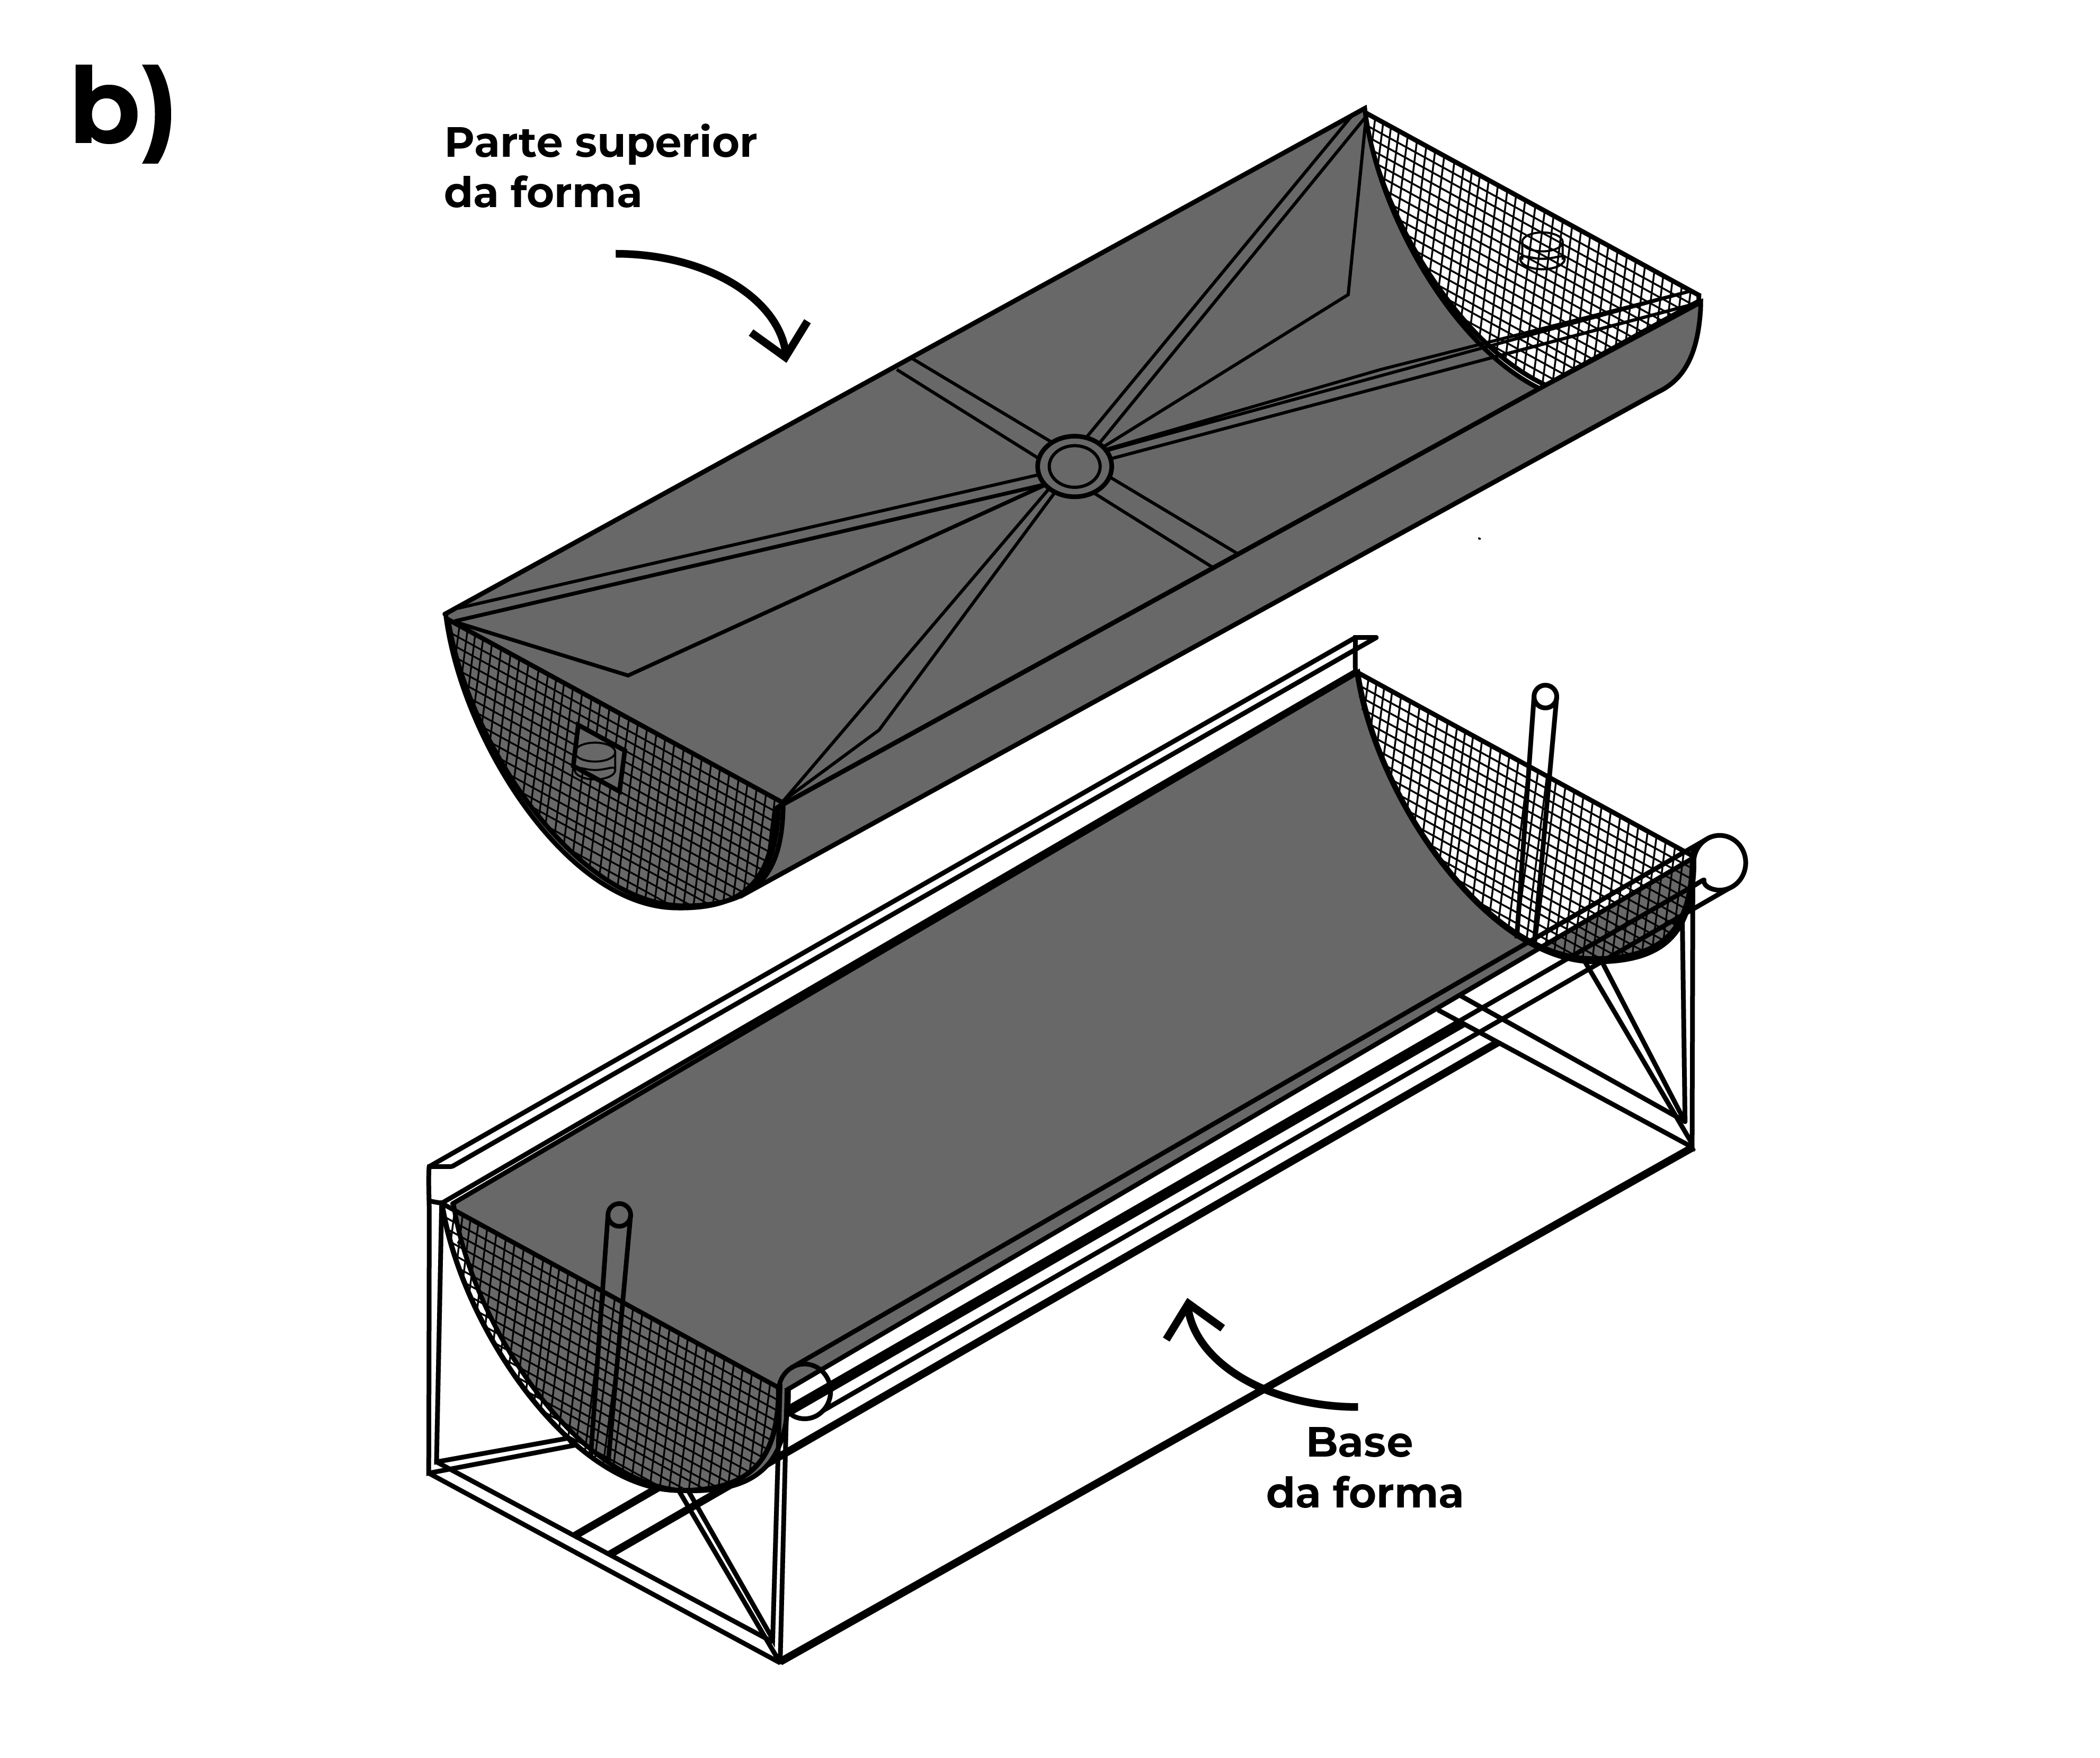
\includegraphics[keepaspectratio]{capitulos/../img/feixes_diagrama.png}}

}

\caption{\label{fig-feixe-diagrama}Diagrama de feixe vivo --- vista em
corte transversal mostrando a instalação em vala rasa.}

\end{figure}%

\end{minipage}%
%
\begin{minipage}{0.50\linewidth}

\begin{figure}[H]

\centering{

\pandocbounded{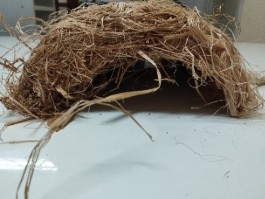
\includegraphics[keepaspectratio]{capitulos/../img/estacas_vivas.jpeg}}

}

\caption{\label{fig-estacas}Estacas vivas detalhadas --- material
vegetativo utilizado para fixação dos feixes.}

\end{figure}%

\end{minipage}%

\end{figure}%

\subsection{Materiais}\label{materiais-1}

A seleção de espécies vegetais para composição dos feixes deve priorizar
ramos com elevada capacidade de brotação vegetativa (capacidade de
emitir raízes e brotos a partir de estacas sem tratamento hormonal),
flexibilidade suficiente para ser curvados e amarrados sem quebrar, e
resistência mecânica mínima para suportar o impacto do escoamento
durante os primeiros meses antes do enraizamento. Os materiais mais
utilizados no Brasil são ramos de sabiá (\emph{Mimosa caesalpiniifolia})
na Caatinga, espécie de alta durabilidade natural (2--3 anos sem
tratamento) e excelente brotação; ramos de gliricídia (\emph{Gliricidia
sepium}) em regiões pantropicais, que enraíza facilmente e fixa
nitrogênio, enriquecendo o solo adjacente; ramos de salgueiro
(\emph{Salix} spp.) em zonas temperadas e subtropicais, escolha
tradicional na bioengenharia europeia, com taxa de brotação superior a
90\%; e bambu verde, de disponibilidade praticamente universal, muito
flexível e de fácil obtenção, embora com menor capacidade de brotação
que as demais espécies.

\subsection{Dimensionamento}\label{dimensionamento-2}

O dimensionamento dos feixes envolve cinco parâmetros interconectados. O
diâmetro do feixe deve situar-se entre 15 e 30 cm, sendo que feixes mais
espessos (25--30 cm) são indicados para encostas com declividade
superior a 15\%, onde a energia do escoamento é maior. O comprimento de
cada segmento deve ser de 2 a 4 m (amarrados com arame galvanizado n.º
18 ou fibra de sisal a cada 50 cm), permitindo manuseio e transporte por
dois trabalhadores. A profundidade da vala corresponde a metade do
diâmetro do feixe (por exemplo, 10 cm para um feixe de 20 cm de
diâmetro), de modo que a metade inferior fique enterrada (garantindo
contato com o solo úmido para brotação) e a metade superior fique
exposta (interceptando o escoamento). O espaçamento entre feixes segue
as curvas de nível, a cada 5--10 m de desnível vertical, com
espaçamentos menores em declividades acentuadas ou em solos de alta
erodibilidade. As estacas de fixação devem ser de material vivo
(gliricídia, sabiá ou salgueiro), com 50 cm de comprimento e diâmetro de
3--5 cm, cravadas a cada 1,0--1,5 m ao longo do feixe e penetrando pelo
menos 30 cm abaixo do fundo da vala.

\subsection{Instalação}\label{instalauxe7uxe3o}

O procedimento de instalação é executado em quatro etapas sequenciais.
Primeiro, traça-se a curva de nível no terreno com auxílio de nível de
mangueira ou clinômetro, marcando a posição da vala. Em seguida,
escava-se a vala rasa ao longo da curva de nível, com largura igual ao
diâmetro do feixe e profundidade equivalente à metade desse diâmetro. O
feixe é então posicionado na vala, com os ramos orientados
transversalmente à direção do escoamento, e fixado com estacas vivas
cravadas através do feixe e no solo abaixo. Por fim, compacta-se terra
contra o feixe no lado montante, assegurando vedação da base e criando
uma pequena ``barreira de solo'' que impede a percolação por baixo nos
primeiros eventos chuvosos, antes que o enraizamento consolide a
estrutura.

\begin{tcolorbox}[enhanced jigsaw, leftrule=.75mm, colframe=quarto-callout-note-color-frame, colback=white, bottomrule=.15mm, opacityback=0, colbacktitle=quarto-callout-note-color!10!white, breakable, bottomtitle=1mm, opacitybacktitle=0.6, title=\textcolor{quarto-callout-note-color}{\faInfo}\hspace{0.5em}{Taxa de sobrevivência}, titlerule=0mm, toprule=.15mm, toptitle=1mm, rightrule=.15mm, left=2mm, arc=.35mm, coltitle=black]

Estudos em encostas de Plintossolo no Nordeste brasileiro demonstraram
taxas de brotação de 70--95\% dos feixes de sabiá após 90 dias da
instalação quando a implantação ocorreu no início da estação chuvosa,
com redução para 30--40\% quando implantados na estação seca. O
posicionamento temporal da instalação é, portanto, tão crítico quanto o
dimensionamento físico.

\end{tcolorbox}

\section{Drenos Verdes}\label{drenos-verdes}

\subsection{Drenos Verdes}\label{drenos-verdes-1}

Os drenos verdes (\emph{vegetated drains} ou \emph{bioswales}) são
canais de drenagem superficial ou subsuperficial revegetados, projetados
para conduzir o escoamento excedente de forma controlada, reduzindo a
velocidade por meio da rugosidade da vegetação e promovendo
simultaneamente a infiltração e a filtração de sedimentos ao longo de
todo o percurso. Enquanto os feixes vivos atuam contra o escoamento
laminar (difuso), os drenos verdes gerenciam o escoamento concentrado
nos talvegues (linhas naturais de convergência do fluxo), constituindo
elementos complementares dentro de um sistema integrado de manejo de
enxurrada.

Diferentemente dos drenos convencionais de concreto, que conduzem a água
em alta velocidade sem nenhuma atenuação de pico ou retenção de
sedimentos, os drenos verdes transformam o canal de drenagem em um
biofiltro linear, onde a vegetação atua como filtro mecânico
(interceptação física de partículas pela folhagem e sistema radicular) e
como redutor de velocidade (aumento do coeficiente de rugosidade de
Manning de 0,013, típico de concreto, para 0,03--0,05 em canais
vegetados).

\subsection{Tipos}\label{tipos}

O dreno superficial vegetado consiste em um canal trapezoidal revestido
com gramíneas de alta densidade (tipicamente \emph{Paspalum notatum},
\emph{Cynodon} spp. ou \emph{Stenotaphrum secundatum}), funcionando como
uma berma vegetada. A velocidade máxima do escoamento deve ser limitada
a 0,5--1,0 m/s para evitar erosão do revestimento vegetal. Para canais
de maior porte, esta técnica evolui para a canaleta verde, cuja
abordagem é desenvolvida em detalhe na \textbf{?@sec-canaleta-verde}.

O dreno subsuperficial biodegradável consiste em um tubo ou camada
drenante composta por materiais vegetais (feixes de bambu, cascas de
coco, fibras de palmeira) enterrados a 30--60 cm de profundidade,
envolvidos em geotêxtil biodegradável (ver \textbf{?@sec-biotexteis}).
Essa configuração cria uma zona preferencial de percolação que drena o
excesso de umidade do solo sem necessidade de tubulação plástica,
degradando-se naturalmente em 3--5 anos, período no qual a drenagem se
estabelece por caminhos preferenciais consolidados no solo.

\begin{figure}

\centering{

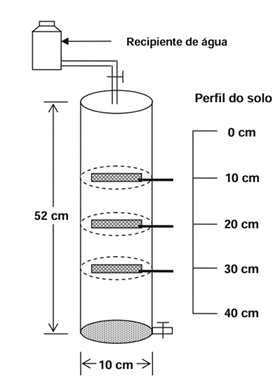
\includegraphics[width=0.75\linewidth,height=\textheight,keepaspectratio]{capitulos/../img/dispositivo_coluna.png}

}

\caption{\label{fig-dispositivo-coluna}Dispositivo de coluna drenante
--- esquema construtivo do dreno subsuperficial biodegradável com
camadas de materiais vegetais envolvidos em geotêxtil.}

\end{figure}%

\subsection{Dimensionamento do Dreno
Superficial}\label{dimensionamento-do-dreno-superficial}

A capacidade de vazão do dreno é calculada pela equação de Manning, que
relaciona a geometria do canal, sua rugosidade e a declividade

\[
Q = \frac{1}{n} \cdot A \cdot R_h^{2/3} \cdot S^{1/2}
\]

onde \(n\) é o coeficiente de rugosidade de Manning (0,03--0,05 para
canais vegetados com gramíneas curtas a médias, podendo chegar a 0,10
para gramíneas altas e densas), \(A\) é a área da seção molhada (m²),
\(R_h\) é o raio hidráulico (razão entre área molhada e perímetro
molhado, em metros) e \(S\) é a declividade longitudinal do canal (m/m).
O dimensionamento inicia com a estimativa da vazão de projeto (método
racional: \(Q = C \cdot i \cdot A\)) e prossegue com a determinação
iterativa da seção transversal que comporta essa vazão com velocidade
inferior a 1,0 m/s.

\subsection{Vantagens dos Drenos
Verdes}\label{vantagens-dos-drenos-verdes}

A Tabela~\ref{tbl-drenos} sintetiza o comparativo técnico-econômico
entre drenos convencionais e drenos verdes, evidenciando as vantagens em
termos de infiltração, filtração, custo e integração paisagística.

\begin{longtable}[]{@{}
  >{\raggedright\arraybackslash}p{(\linewidth - 4\tabcolsep) * \real{0.1731}}
  >{\raggedright\arraybackslash}p{(\linewidth - 4\tabcolsep) * \real{0.5769}}
  >{\raggedright\arraybackslash}p{(\linewidth - 4\tabcolsep) * \real{0.2500}}@{}}
\caption{Comparativo entre drenos convencionais e drenos
verdes.}\label{tbl-drenos}\tabularnewline
\toprule\noalign{}
\begin{minipage}[b]{\linewidth}\raggedright
Aspecto
\end{minipage} & \begin{minipage}[b]{\linewidth}\raggedright
Dreno convencional (concreto)
\end{minipage} & \begin{minipage}[b]{\linewidth}\raggedright
Dreno verde
\end{minipage} \\
\midrule\noalign{}
\endfirsthead
\toprule\noalign{}
\begin{minipage}[b]{\linewidth}\raggedright
Aspecto
\end{minipage} & \begin{minipage}[b]{\linewidth}\raggedright
Dreno convencional (concreto)
\end{minipage} & \begin{minipage}[b]{\linewidth}\raggedright
Dreno verde
\end{minipage} \\
\midrule\noalign{}
\endhead
\bottomrule\noalign{}
\endlastfoot
Infiltração & Nula (superfície impermeável) & 30--60\% do volume \\
Filtração de sedimentos & Nenhuma & 50--80\% \\
Custo de implantação & R\$ 200--500/m & R\$ 40--100/m \\
Manutenção & Limpeza mecânica (semestral) & Roçada periódica
(trimestral) \\
Paisagem & Impacto visual negativo & Integrado ao ambiente \\
Vida útil & 30--50 anos & Indefinida (autorrenovável) \\
\end{longtable}

\begin{tcolorbox}[enhanced jigsaw, leftrule=.75mm, colframe=quarto-callout-tip-color-frame, colback=white, bottomrule=.15mm, opacityback=0, colbacktitle=quarto-callout-tip-color!10!white, breakable, bottomtitle=1mm, opacitybacktitle=0.6, title=\textcolor{quarto-callout-tip-color}{\faLightbulb}\hspace{0.5em}{Aplicação ideal}, titlerule=0mm, toprule=.15mm, toptitle=1mm, rightrule=.15mm, left=2mm, arc=.35mm, coltitle=black]

Drenos verdes são especialmente eficazes em áreas periurbanas
(loteamentos, campi universitários, parques industriais) e estradas
rurais, onde a infraestrutura convencional de concreto é cara, pouco
sustentável e esteticamente desarmônica. Em projetos de Soluções
Baseadas na Natureza (ver \textbf{?@sec-nbs}), os drenos verdes são
frequentemente combinados com jardins de chuva e tetos verdes para
compor sistemas de drenagem urbana sustentável (SUDS).

\end{tcolorbox}

\section{Integração Feixes +
Drenos}\label{integrauxe7uxe3o-feixes-drenos}

A combinação de feixes vivos ao longo de curvas de nível com drenos
verdes nos talvegues cria um sistema integrado de manejo de enxurrada
que opera em três escalas funcionais complementares. Na escala de
encosta, os feixes interceptam o escoamento laminar difuso, reduzindo
sua velocidade e promovendo a deposição de sedimentos finos, de modo que
a água que atinge os talvegues já chega com menor carga sólida e menor
energia cinética. Na escala dos talvegues, os drenos verdes recebem o
escoamento concentrado remanescente e o conduzem de forma controlada até
o exutório, infiltrando 30--60\% do volume e filtrando 50--80\% dos
sedimentos restantes. Na escala de bacia, a integração dos dois sistemas
reduz a conectividade hidrossedimentológica entre as vertentes e os
corpos d'água receptores, diminuindo simultaneamente o pico de vazão
(amortecimento) e a carga sólida total exportada.

\begin{figure}

\centering{

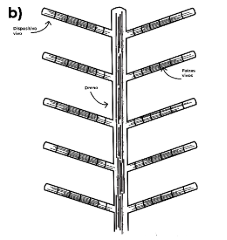
\includegraphics[width=0.8\linewidth,height=\textheight,keepaspectratio]{capitulos/../img/espinha_peixe.png}

}

\caption{\label{fig-espinha-peixe}Arranjo em espinha de peixe
(\emph{herringbone}) --- disposição espacial dos feixes vivos em curvas
de nível combinados com drenos verdes nos talvegues, formando o sistema
integrado de manejo de enxurrada.}

\end{figure}%

A complementaridade dos dois sistemas é sinérgica: os feixes protegem os
drenos de obstrução por excesso de sedimentos, enquanto os drenos
protegem os feixes de sobrecarga por concentração de escoamento,
garantindo que cada componente opere dentro de sua faixa de projeto.
Esse arranjo integrado é particularmente eficaz em encostas longas
(\textgreater{} 100 m de comprimento de rampa) onde nenhuma das duas
técnicas, isoladamente, seria suficiente para controlar o escoamento e a
erosão de forma satisfatória.

\chapter{Hidrossemeadura}\label{hidrossemeadura-1}

\# Hidrossemeadura \{\#sec-hidrossemeadura\}

A hidrossemeadura (\emph{hydroseeding} ou \emph{hydraulic mulch
seeding}) é a técnica de projeção mecanizada de uma mistura aquosa
contendo sementes, mulch (cobertura morta), fertilizante e fixador
(\emph{tackifier}) sobre taludes e superfícies erodíveis. O princípio
consiste em aplicar, simultaneamente e de forma homogênea, todos os
insumos necessários para o estabelecimento vegetal em um único passo
operacional, utilizando um equipamento (hidrossemeador) que projeta a
pasta sob pressão a distâncias de 30 a 60 m. Essa abordagem elimina a
necessidade de acesso direto a superfícies íngremes, o que torna a
hidrossemeadura particularmente adequada para taludes rodoviários,
barragens, pedreiras, aterros sanitários e áreas de mineração onde o
plantio manual seria impraticável ou perigoso.

Em termos de produtividade, a hidrossemeadura é a técnica mais eficiente
de revegetação de grandes áreas, alcançando até 5.000 m²/h com
equipamentos de grande porte, cifra que se compara aos 50--100 m²/h do
plantio manual de mudas e aos 200--500 m²/h da semeadura a lanço. Essa
diferença de escala explica por que a hidrossemeadura domina o mercado
de revegetação de obras lineares (rodovias, ferrovias, gasodutos, linhas
de transmissão) em todo o mundo. A Figura~\ref{fig-hidrossemeadura}
mostra a aplicação da técnica em um talude rodoviário, onde é possível
observar o jato de projeção da pasta verde (a coloração distingue-se da
superfície do solo, permitindo ao operador controlar visualmente a
uniformidade de cobertura).

\begin{figure}

\centering{

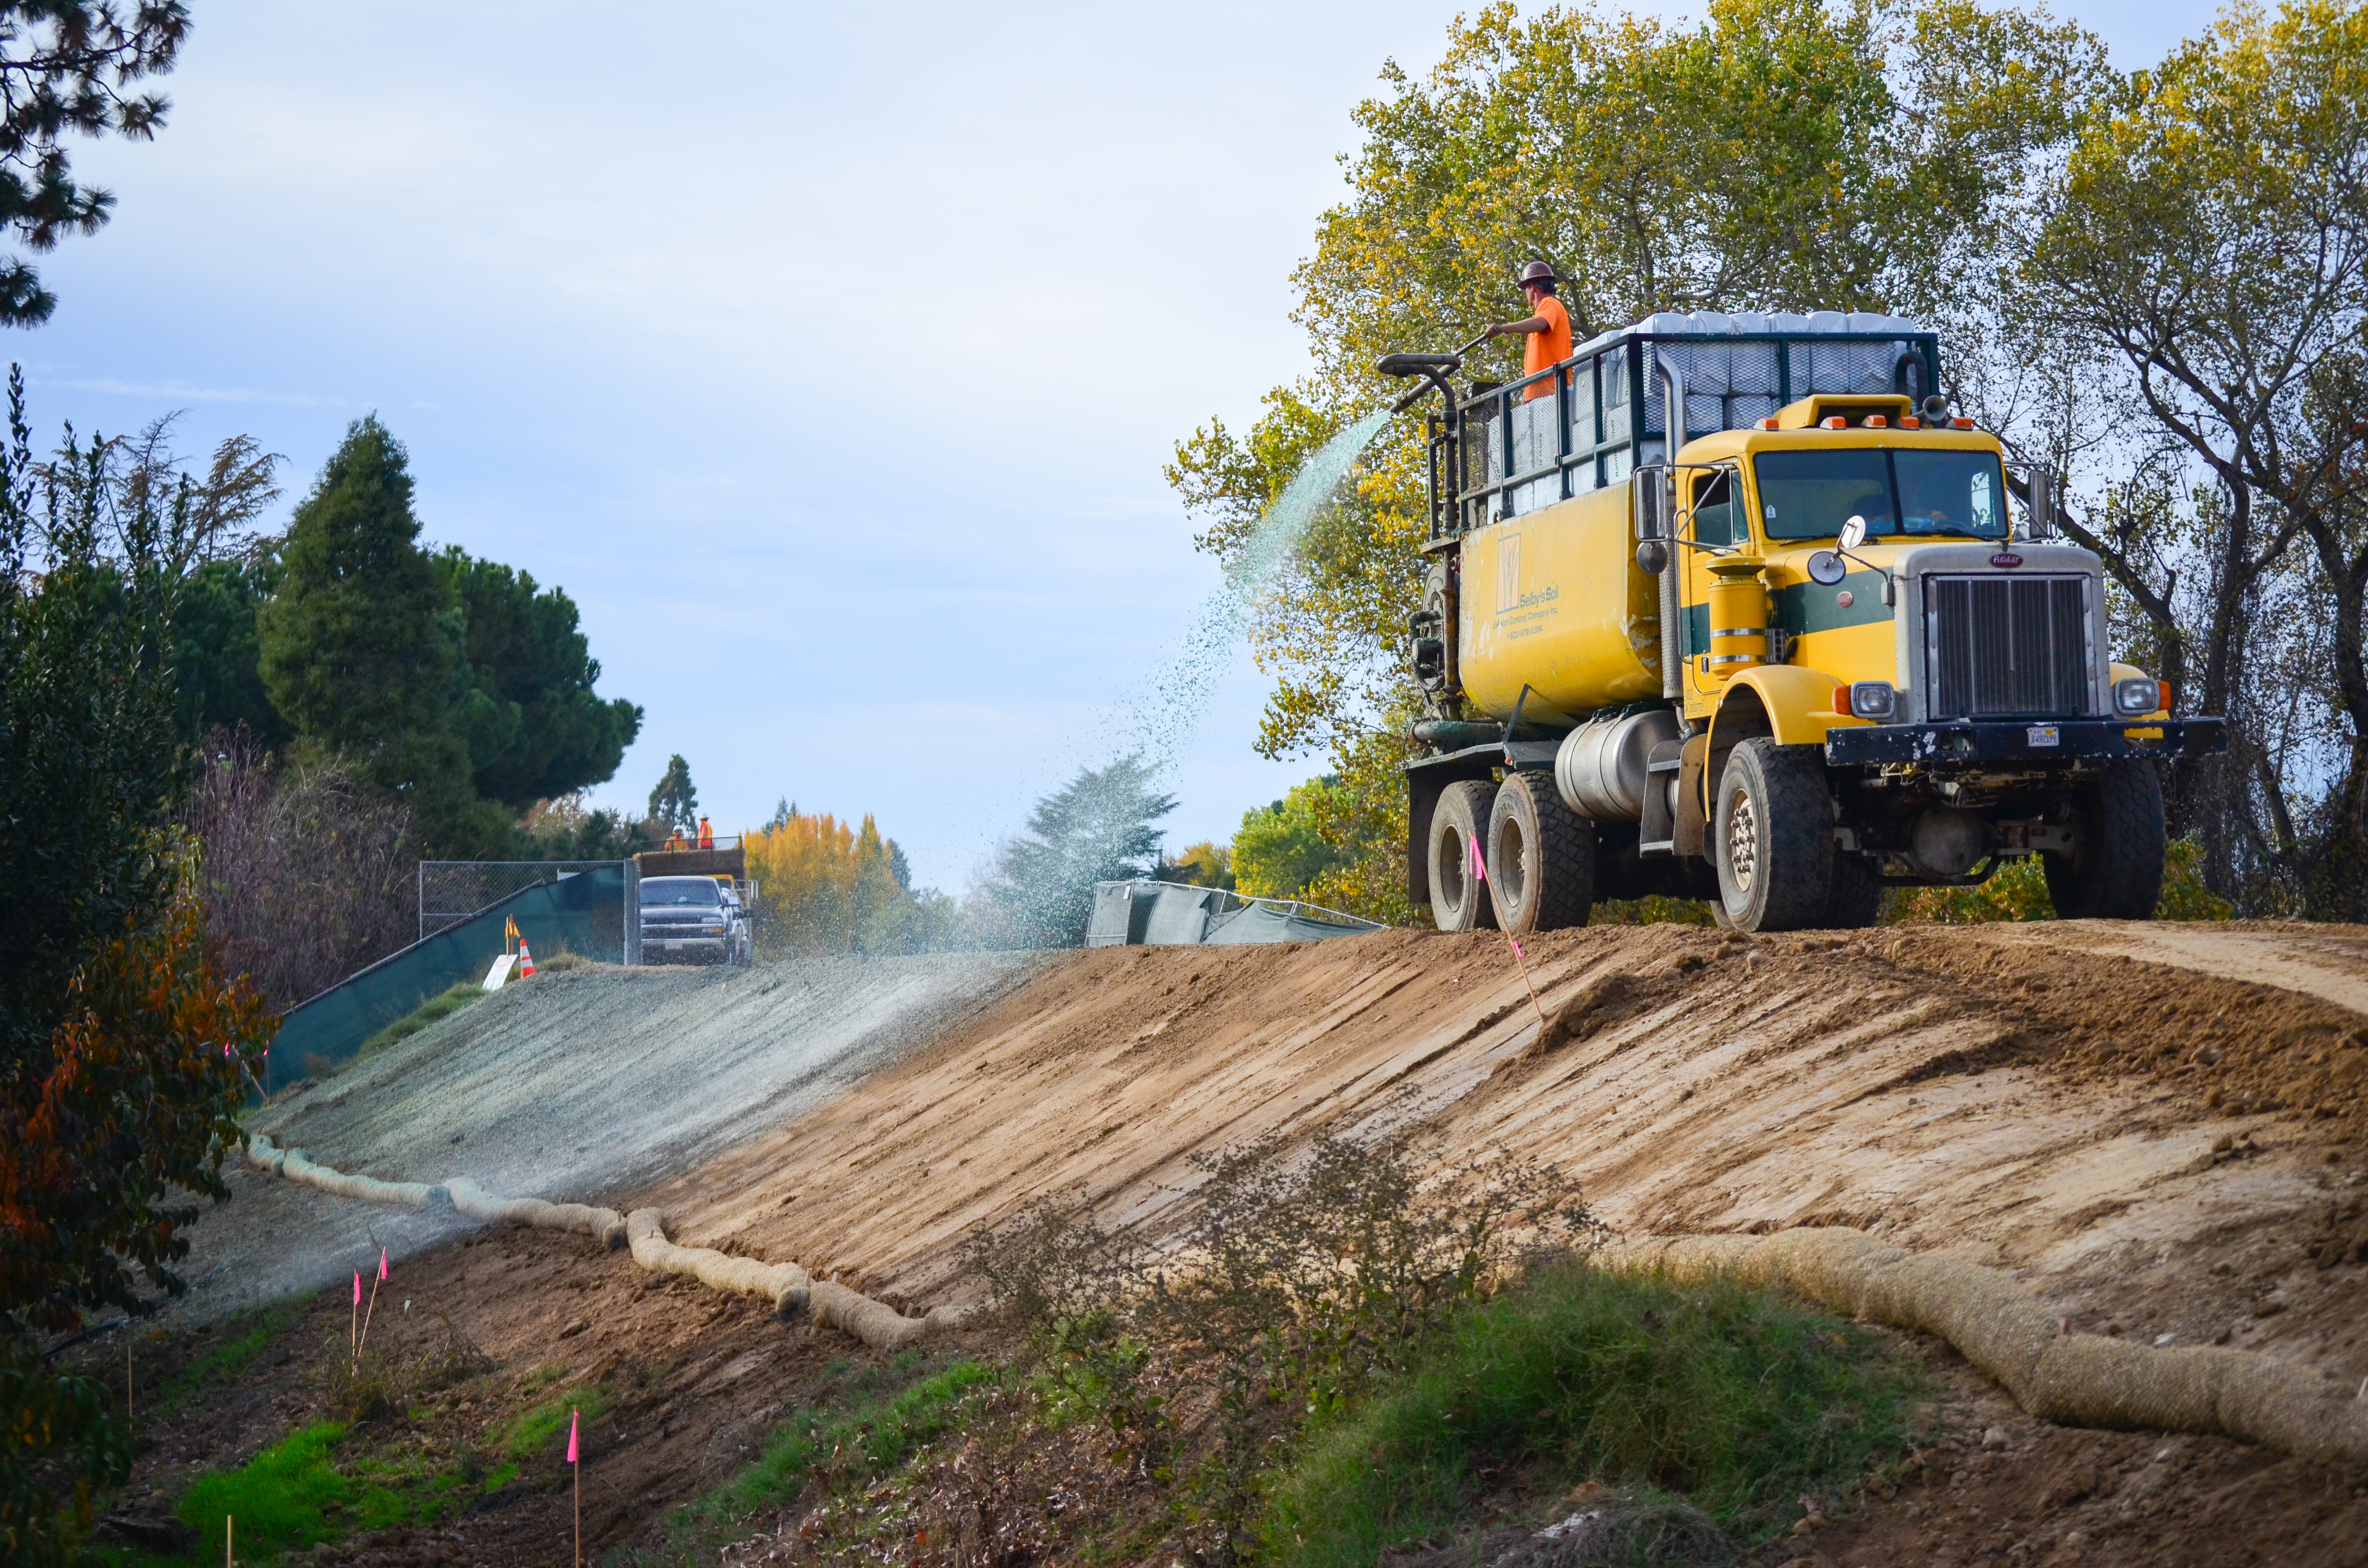
\includegraphics[width=0.8\linewidth,height=\textheight,keepaspectratio]{capitulos/../img/hidrossemeadura_levee.jpg}

}

\caption{\label{fig-hidrossemeadura}Aplicação de hidrossemeadura em
talude rodoviário --- projeção mecanizada da pasta com sementes, mulch e
fertilizante.}

\end{figure}%

O resultado prático da aplicação pode ser observado em duas situações
distintas. A Figura~\ref{fig-hidro-restauracao} mostra a projeção da
pasta em uma área degradada em processo de restauração, enquanto a
Figura~\ref{fig-hidro-rodovia} apresenta o resultado após o
estabelecimento vegetal, com gramíneas já consolidadas em talude de alta
declividade, demonstrando a eficácia da técnica mesmo em superfícies com
inclinação superior a 45°.

\begin{figure}

\begin{minipage}{0.50\linewidth}

\begin{figure}[H]

\centering{

\pandocbounded{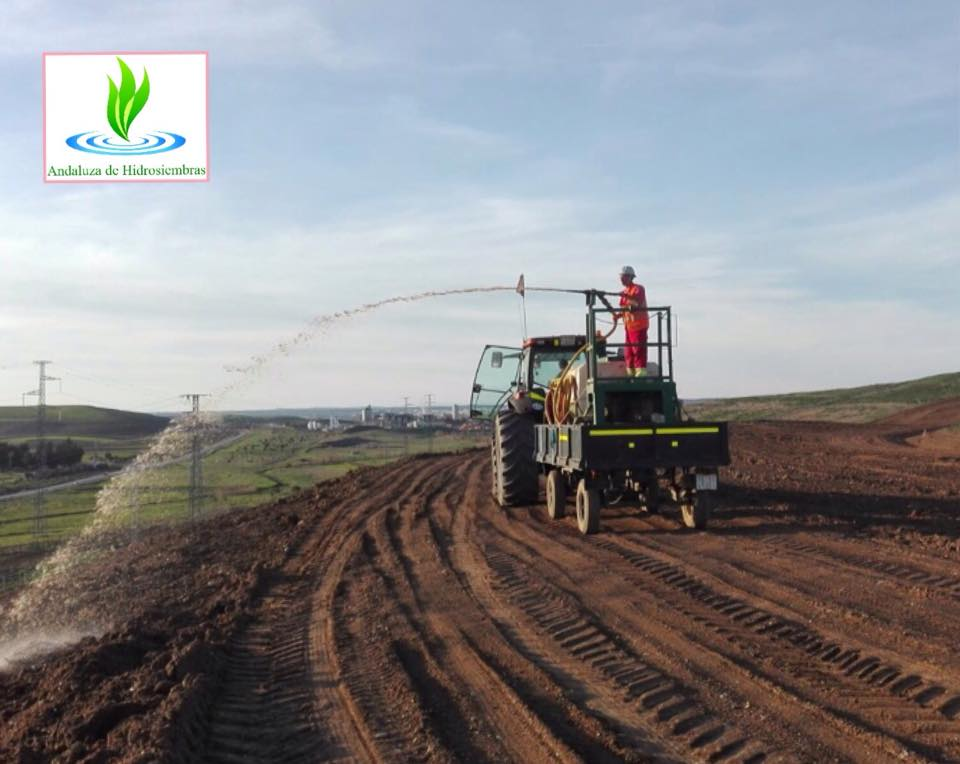
\includegraphics[keepaspectratio]{capitulos/../img/hidrossemeadura_restauracao.jpg}}

}

\caption{\label{fig-hidro-restauracao}Hidrossemeadura em restauração de
área degradada --- projeção da pasta sobre superfície erodível.}

\end{figure}%

\end{minipage}%
%
\begin{minipage}{0.50\linewidth}

\begin{figure}[H]

\centering{

\pandocbounded{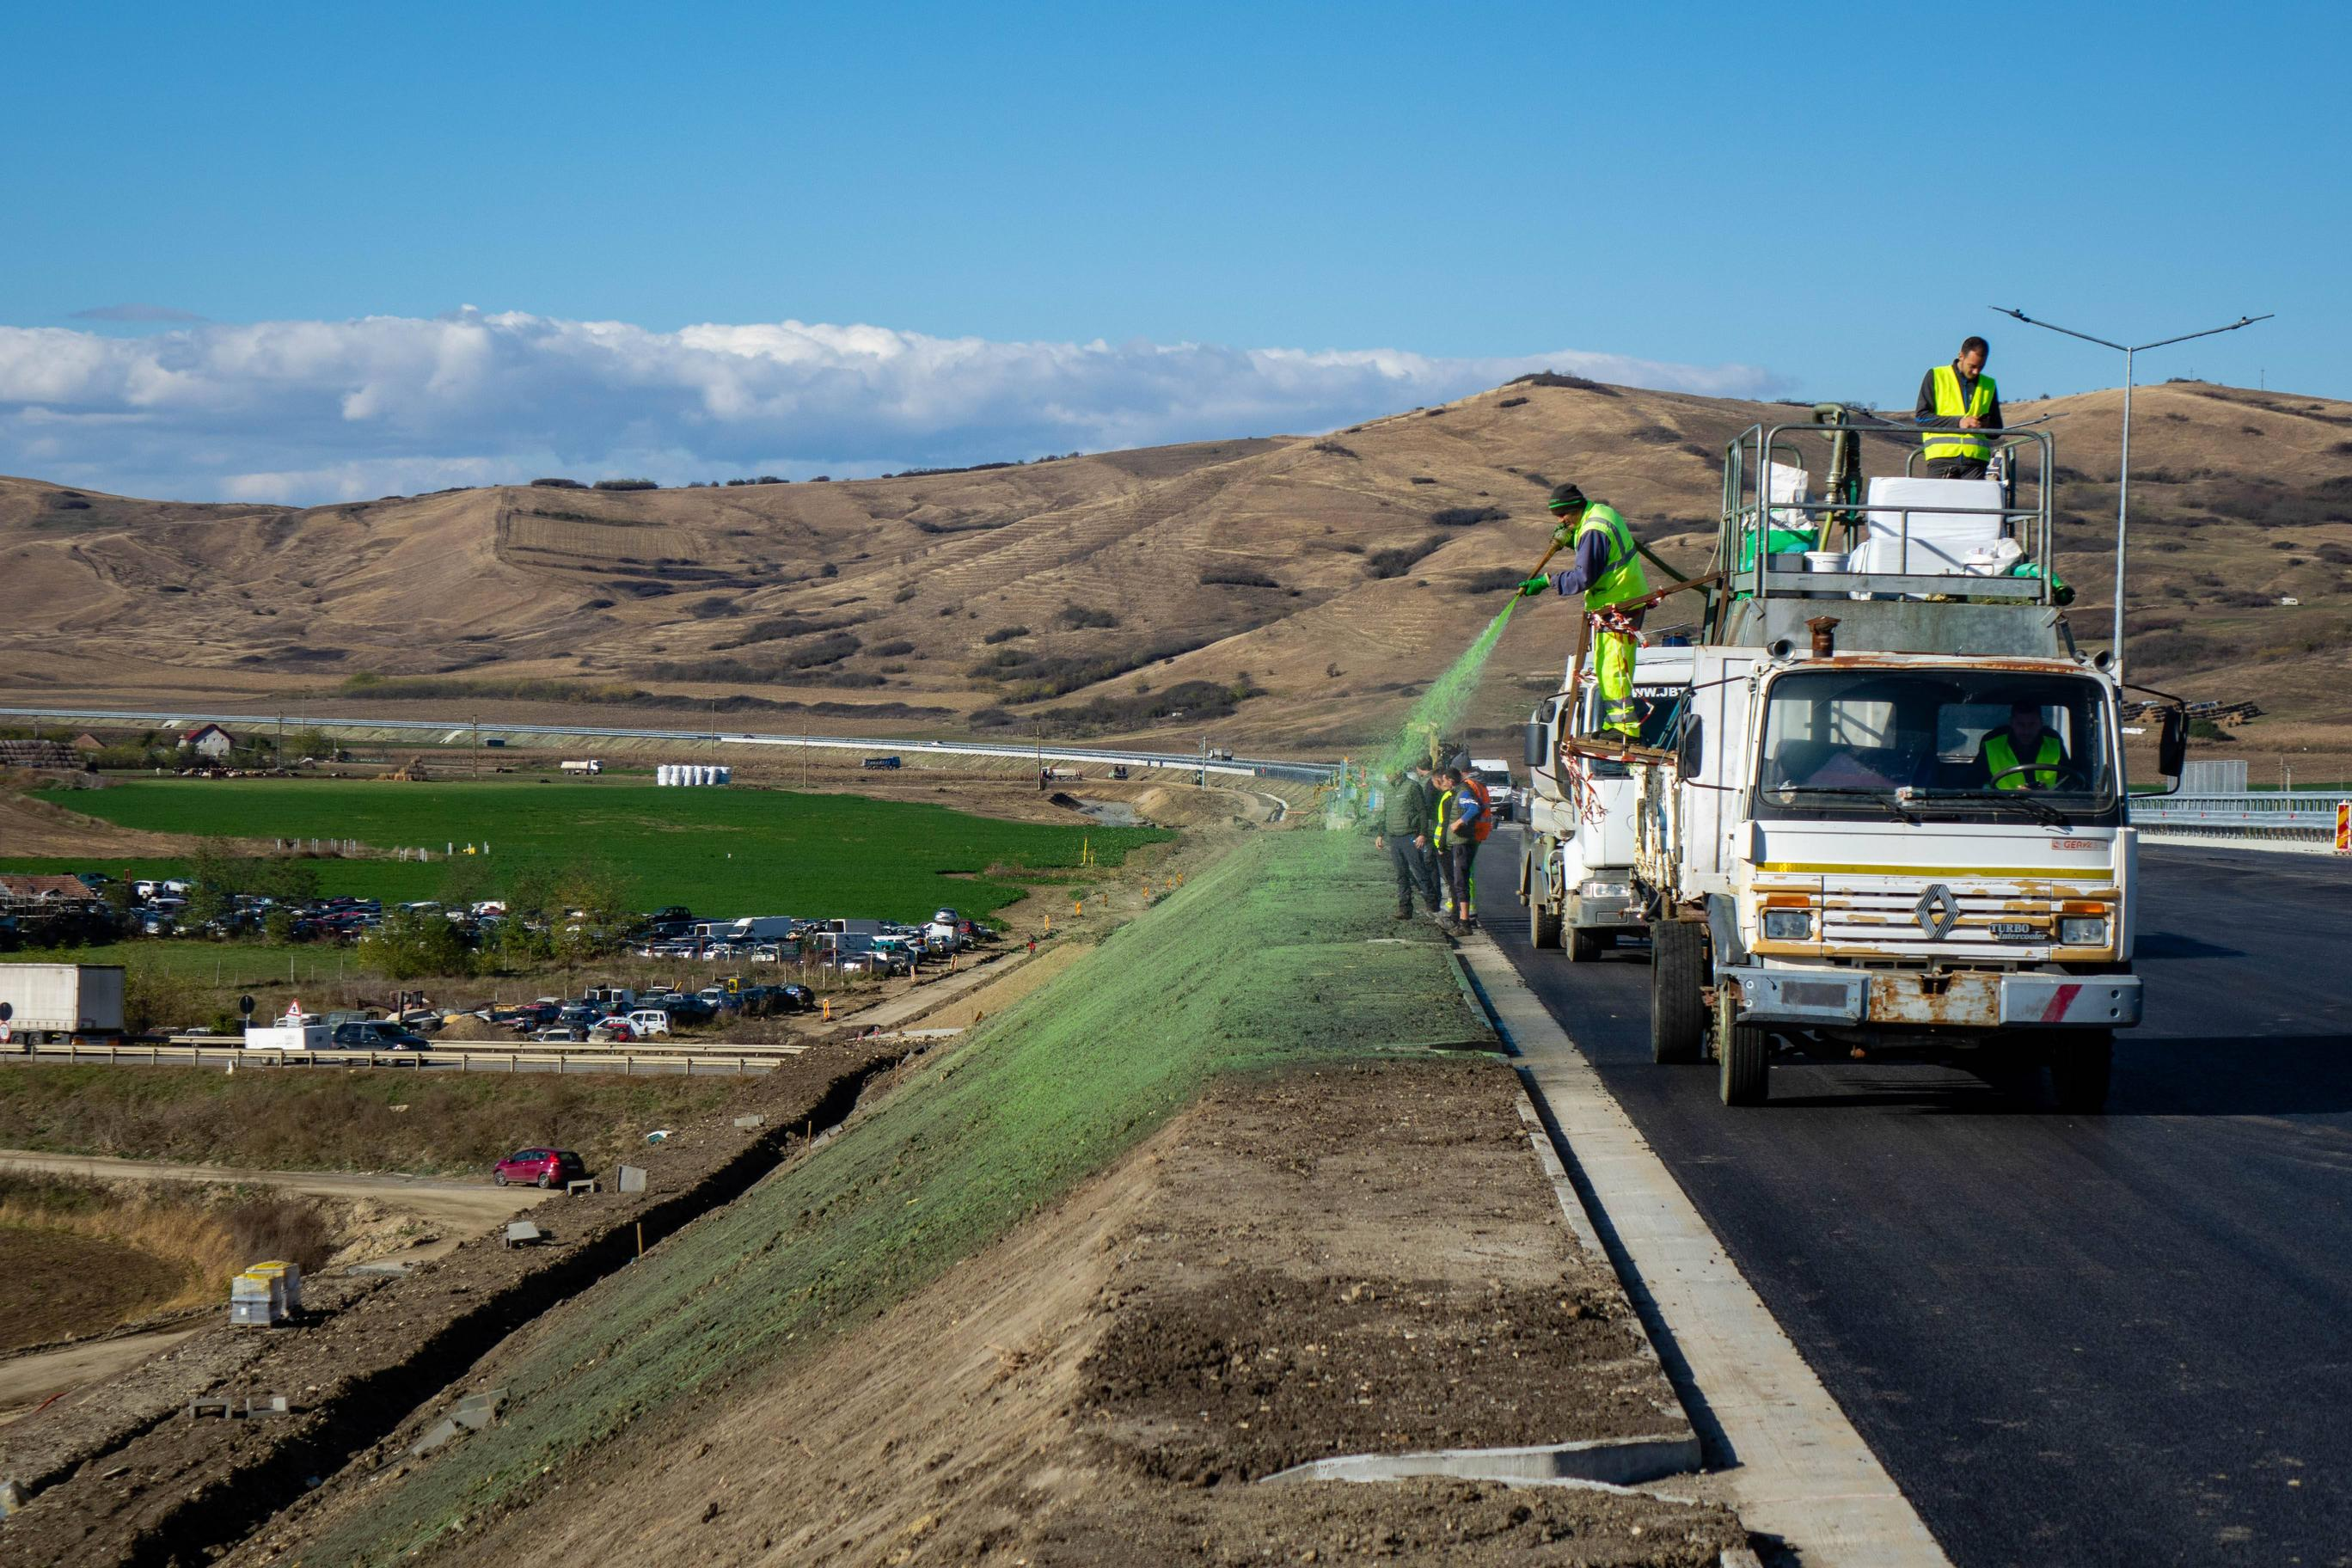
\includegraphics[keepaspectratio]{capitulos/../img/hidrossemeadura_rodovia.jpg}}

}

\caption{\label{fig-hidro-rodovia}Resultado da hidrossemeadura em
rodovia --- vegetação herbácea estabelecida em talude com alta
declividade.}

\end{figure}%

\end{minipage}%

\end{figure}%

\section{Composição da Pasta}\label{composiuxe7uxe3o-da-pasta}

A pasta de hidrossemeadura é uma suspensão aquosa cujos componentes
desempenham funções complementares e sinérgicas. A formulação é ajustada
conforme o tipo de solo, a declividade, o regime climático e os
objetivos de revegetação. A Tabela~\ref{tbl-pasta} apresenta a
composição típica e a dosagem de cada componente.

\begin{longtable}[]{@{}
  >{\raggedright\arraybackslash}p{(\linewidth - 4\tabcolsep) * \real{0.3429}}
  >{\raggedright\arraybackslash}p{(\linewidth - 4\tabcolsep) * \real{0.2286}}
  >{\raggedright\arraybackslash}p{(\linewidth - 4\tabcolsep) * \real{0.4286}}@{}}
\caption{Composição típica da pasta de
hidrossemeadura.}\label{tbl-pasta}\tabularnewline
\toprule\noalign{}
\begin{minipage}[b]{\linewidth}\raggedright
Componente
\end{minipage} & \begin{minipage}[b]{\linewidth}\raggedright
Função
\end{minipage} & \begin{minipage}[b]{\linewidth}\raggedright
Dosagem típica
\end{minipage} \\
\midrule\noalign{}
\endfirsthead
\toprule\noalign{}
\begin{minipage}[b]{\linewidth}\raggedright
Componente
\end{minipage} & \begin{minipage}[b]{\linewidth}\raggedright
Função
\end{minipage} & \begin{minipage}[b]{\linewidth}\raggedright
Dosagem típica
\end{minipage} \\
\midrule\noalign{}
\endhead
\bottomrule\noalign{}
\endlastfoot
Água & Veículo e hidratação inicial das sementes & 2.000--4.000 L/ha \\
Sementes & Estabelecimento de cobertura vegetal & 50--200 kg/ha \\
Mulch & Proteção superficial contra impacto de gotas e dessecação &
1.500--3.000 kg/ha \\
Fertilizante & Nutrição inicial (N--P--K + micronutrientes) & 200--500
kg/ha \\
Fixador (\emph{tackifier}) & Adesão da pasta ao solo e resistência à
erosão hídrica & 50--150 kg/ha \\
Corante & Controle visual de uniformidade de aplicação & 5--10 L/ha \\
\end{longtable}

A água atua como veículo para homogeneizar e projetar os demais
componentes, além de fornecer a umidade inicial para ativação da
germinação. O mulch é o componente de maior massa, sendo responsável por
proteger a superfície contra o impacto cinético das gotas de chuva
(\emph{splash erosion}), manter a umidade superficial e criar um
microclima favorável à germinação. O fertilizante fornece nutrientes de
liberação lenta (formulação 10-10-10 ou 20-05-20) para sustentar o
crescimento vegetal nos primeiros 60--90 dias, período em que as raízes
ainda não acessam os nutrientes do solo. O fixador é um polímero
(natural ou sintético) que aglutina as partículas de mulch e sementes ao
solo, impedindo que a pasta seja lavada pela primeira chuva após a
aplicação. O corante (verde, à base de clorofila sintética) permite ao
operador identificar visualmente as áreas já cobertas, evitando
sobreposição ou omissão.

\section{Tipos de Mulch}\label{tipos-de-mulch}

A escolha do mulch é uma das decisões mais críticas do projeto de
hidrossemeadura, pois determina o nível de proteção superficial, o tempo
de degradação e, consequentemente, a janela de vulnerabilidade entre a
aplicação e o estabelecimento vegetal efetivo.

\subsection{Mulch de Celulose}\label{mulch-de-celulose}

O mulch de celulose é composto por fibras de papel reciclado ou celulose
virgem moída. Apresenta retenção hídrica moderada (retém 6--8× seu peso
em água) e degradação rápida (30--60 dias em clima tropical úmido). Seu
custo é o mais baixo entre os mulches comerciais (R\$ 3--6/kg), o que o
torna a escolha padrão para projetos de grande escala em declividades
moderadas (\textless{} 30°). A principal limitação é a baixa resistência
à erosão hídrica: em taludes íngremes, a chuva intensa pode remover o
mulch de celulose antes que a germinação esteja consolidada.

\subsection{Mulch de Madeira}\label{mulch-de-madeira}

O mulch de madeira é composto por fibras de madeira processada
(eucalipto, pinus), com fibras mais longas e interconectadas que o de
celulose. Oferece retenção hídrica elevada (10--12× seu peso),
degradação lenta (90--180 dias) e maior resistência à erosão, sendo
indicado para taludes com declividade de 30--45° ou em regiões com
chuvas intensas. Seu custo (R\$ 5--10/kg) é intermediário, equilibrando
proteção e economia.

\subsection{Mulch Bonded Fiber Matrix
(BFM)}\label{mulch-bonded-fiber-matrix-bfm}

O BFM representa a categoria premium de mulch, combinando fibras longas
de madeira com aglutinante biodegradável que, ao secar, forma uma manta
coesa sobre o solo. Essa manta pode ser suficientemente resistente para
substituir biomantas têxteis (ver \textbf{?@sec-biomantas}) em taludes
de até 45°, com a vantagem de aplicação por projeção (sem necessidade de
desenrolar e fixar rolos manualmente). O custo é o mais elevado (R\$
8--15/kg), justificado em projetos onde a logística de instalação de
biomantas é inviável (acessos difíceis, grandes extensões de taludes).

\section{\texorpdfstring{Fixadores
(\emph{Tackifiers})}{Fixadores (Tackifiers)}}\label{fixadores-tackifiers}

Os fixadores são o componente que garante a permanência da pasta
aplicada sobre a superfície do solo diante das forças erosivas da chuva
e do escoamento. A Tabela~\ref{tbl-fixadores} compara os quatro tipos
mais utilizados no mercado brasileiro.

\begin{longtable}[]{@{}lllll@{}}
\caption{Tipos de fixadores e suas
propriedades.}\label{tbl-fixadores}\tabularnewline
\toprule\noalign{}
Tipo & Origem & Resistência à chuva & Duração & Custo (R\$/kg) \\
\midrule\noalign{}
\endfirsthead
\toprule\noalign{}
Tipo & Origem & Resistência à chuva & Duração & Custo (R\$/kg) \\
\midrule\noalign{}
\endhead
\bottomrule\noalign{}
\endlastfoot
Guar & Vegetal (goma de guar) & Moderada & 30--60 dias & 15--25 \\
Psyllium & Vegetal (\emph{Plantago}) & Alta & 60--90 dias & 25--40 \\
PAM (poliacrilamida) & Sintético & Muito alta & 90--180 dias & 30--50 \\
Amido & Vegetal (milho/mandioca) & Baixa & 15--30 dias & 8--15 \\
\end{longtable}

A escolha do fixador depende do regime pluviométrico local e da
declividade do talude. Em regiões com chuvas intensas e frequentes
(pluviosidade \textgreater{} 1.500 mm/ano), fixadores sintéticos (PAM)
ou de alta resistência (psyllium) são recomendados. Em regiões
semiáridas, onde o risco de lavagem é menor, o amido ou guar oferecem
boa relação custo-eficácia.

\section{Dimensionamento}\label{dimensionamento-3}

\subsection{Taxa de Aplicação}\label{taxa-de-aplicauxe7uxe3o}

A taxa de aplicação (\(T_a\)) é a quantidade total de mulch a ser
aplicada por unidade de área, ajustada por fatores multiplicadores que
expressam as condições do sítio

\[
T_a = T_{base} \cdot F_d \cdot F_s \cdot F_c
\]

onde \(T_{base}\) é a taxa base de 3.000 kg/ha (estabelecida para
gramíneas em taludes de até 30° em solo argiloso e clima úmido), \(F_d\)
é o fator de declividade (1,0 para inclinações inferiores a 30°, 1,3
para 30--45° e 1,6 para ângulos superiores a 45°, refletindo o aumento
da energia erosiva com o gradiente), \(F_s\) é o fator de solo (1,0 para
argilosos, que possuem maior coesão, 1,2 para arenosos e 1,4 para
siltosos, que são os mais erodíveis) e \(F_c\) é o fator climático (1,0
para clima úmido com chuvas distribuídas e 1,3 para semiárido onde a
concentração de chuvas intensas em curtos períodos eleva o risco de
lavagem).

\subsection{Mistura de Sementes}\label{mistura-de-sementes}

A composição da mistura de sementes deve atender a três funções
temporais complementares. A fração de estabelecimento rápido (70\% da
mistura) compreende gramíneas de germinação acelerada, como
\emph{Brachiaria decumbens}, \emph{Brachiaria brizantha} cv. Marandu e
\emph{Paspalum notatum}, cujas plântulas emergem em 5--15 dias e
proporcionam cobertura mínima de 40\% em 30 dias. A fração de fixação
biológica de nitrogênio (20\%) inclui leguminosas como
\emph{Stylosanthes} spp., \emph{Cajanus cajan} (guandu) e
\emph{Crotalaria juncea}, que fixam 50--200 kg N/ha/ano via simbiose com
rizóbios, reduzindo a dependência de fertilizantes minerais a médio
prazo. A fração de persistência (10\%) contempla gramíneas perenes de
ciclo longo e raízes profundas, que assumem a proteção do solo após a
senescência das espécies pioneiras, garantindo cobertura permanente.

\section{Equipamentos}\label{equipamentos}

O hidrossemeador mecânico é o equipamento central da técnica,
consistindo em um tanque cilíndrico de aço ou polietileno com capacidade
de 2.000 a 8.000 L, equipado com agitador mecânico interno (para manter
a pasta homogênea), bomba centrífuga de alta pressão e canhão de
projeção direcional. A pressão de trabalho situa-se entre 4 e 8 bar,
gerando um jato com alcance de 30 a 60 m dependendo da viscosidade da
pasta e da configuração do bico. O rendimento típico é de 3.000--5.000
m²/h para equipamentos montados em caminhão (os mais comuns no Brasil),
podendo chegar a 8.000 m²/h em hidrossemeadores de grande porte montados
em carretas. Para áreas de difícil acesso (morros, encostas sem
estrada), existem hidrossemeadores portáteis montados em trailers leves
(500--1.000 L) ou mochilas motorizadas (50--100 L), com rendimento
inferior (500--1.000 m²/h) mas grande versatilidade operacional.

A calibração do equipamento antes de cada aplicação é fundamental: o
operador deve ajustar a velocidade do agitador para evitar sedimentação
das sementes no fundo do tanque, regular a pressão para obter o alcance
desejado sem fragmentar as sementes pelo impacto excessivo, e verificar
a uniformidade da distribuição por meio de testes em área controlada.

\section{Monitoramento}\label{monitoramento}

O monitoramento pós-aplicação é indispensável para avaliar o sucesso da
hidrossemeadura e identificar precocemente eventuais falhas que exijam
reaplicação. A Tabela~\ref{tbl-monitoramento} estabelece as metas
quantitativas para cada indicador nos primeiros 90 dias.

\begin{longtable}[]{@{}llll@{}}
\caption{Metas de monitoramento
pós-hidrossemeadura.}\label{tbl-monitoramento}\tabularnewline
\toprule\noalign{}
Indicador & Meta (30 dias) & Meta (60 dias) & Meta (90 dias) \\
\midrule\noalign{}
\endfirsthead
\toprule\noalign{}
Indicador & Meta (30 dias) & Meta (60 dias) & Meta (90 dias) \\
\midrule\noalign{}
\endhead
\bottomrule\noalign{}
\endlastfoot
Germinação & \textgreater{} 50\% & --- & --- \\
Cobertura & \textgreater{} 40\% & \textgreater{} 70\% & \textgreater{}
90\% \\
Erosão visível & \textless{} 5\% da área & \textless{} 2\% & 0\% \\
\end{longtable}

Áreas que não atingirem a meta de 40\% de cobertura aos 30 dias devem
ser avaliadas quanto à causa da falha (drenagem do fixador, predação de
sementes, temperatura inadequada, déficit hídrico) e submetidas a
reaplicação localizada. A reaplicação total é indicada apenas quando a
cobertura for inferior a 20\% aos 30 dias, sugerindo falha sistêmica na
formulação ou na aplicação.

\section{Custos}\label{custos-1}

A Tabela~\ref{tbl-custos-hidro} sintetiza os custos médios de
hidrossemeadura em comparação com o plantio manual de mudas e a
semeadura a lanço, evidenciando a vantagem competitiva da técnica em
projetos de grande escala.

\begin{longtable}[]{@{}
  >{\raggedright\arraybackslash}p{(\linewidth - 6\tabcolsep) * \real{0.1053}}
  >{\raggedright\arraybackslash}p{(\linewidth - 6\tabcolsep) * \real{0.2807}}
  >{\raggedright\arraybackslash}p{(\linewidth - 6\tabcolsep) * \real{0.2807}}
  >{\raggedright\arraybackslash}p{(\linewidth - 6\tabcolsep) * \real{0.3333}}@{}}
\caption{Comparativo de custos e produtividade entre métodos de
revegetação.}\label{tbl-custos-hidro}\tabularnewline
\toprule\noalign{}
\begin{minipage}[b]{\linewidth}\raggedright
Item
\end{minipage} & \begin{minipage}[b]{\linewidth}\raggedright
Hidrossemeadura
\end{minipage} & \begin{minipage}[b]{\linewidth}\raggedright
Plantio manual
\end{minipage} & \begin{minipage}[b]{\linewidth}\raggedright
Semeadura a lanço
\end{minipage} \\
\midrule\noalign{}
\endfirsthead
\toprule\noalign{}
\begin{minipage}[b]{\linewidth}\raggedright
Item
\end{minipage} & \begin{minipage}[b]{\linewidth}\raggedright
Hidrossemeadura
\end{minipage} & \begin{minipage}[b]{\linewidth}\raggedright
Plantio manual
\end{minipage} & \begin{minipage}[b]{\linewidth}\raggedright
Semeadura a lanço
\end{minipage} \\
\midrule\noalign{}
\endhead
\bottomrule\noalign{}
\endlastfoot
Insumos & R\$ 8.000--15.000/ha & R\$ 12.000--25.000/ha & R\$
3.000--6.000/ha \\
Mão de obra & R\$ 1.000--3.000/ha & R\$ 8.000--15.000/ha & R\$
2.000--4.000/ha \\
Total & R\$ 9.000--18.000/ha & R\$ 20.000--40.000/ha & R\$
5.000--10.000/ha \\
Produtividade & 3.000--5.000 m²/h & 50--100 m²/h & 200--500 m²/h \\
Aplicabilidade em taludes & Até 70° & Até 30° & Até 15° \\
\end{longtable}

\section{Limitações e
Contraindicações}\label{limitauxe7uxf5es-e-contraindicauxe7uxf5es}

Apesar de sua versatilidade, a hidrossemeadura não é indicada em todas
as situações. Em solos rochosos sem substrato (rocha exposta com
\textless{} 5 cm de solo), a pasta não adere adequadamente e as raízes
não encontram meio para se desenvolver, exigindo prévia aplicação de
substrato orgânico ou tela metálica ancorada na rocha. Em taludes com
erosão ativa (presença de sulcos ou ravinas), a pasta será removida pelo
escoamento concentrado antes da germinação, sendo necessário primeiro
estabilizar as feições erosivas com paliçadas (ver
\textbf{?@sec-palicadas}) ou biomantas (ver \textbf{?@sec-biomantas}) e
depois aplicar a hidrossemeadura nas áreas entre elas. Em períodos de
seca prolongada, a germinação será nula ou insignificante, resultando em
perda total dos insumos aplicados, razão pela qual o planejamento
temporal da aplicação deve coincidir com o início da estação chuvosa.

\begin{tcolorbox}[enhanced jigsaw, leftrule=.75mm, colframe=quarto-callout-warning-color-frame, colback=white, bottomrule=.15mm, opacityback=0, colbacktitle=quarto-callout-warning-color!10!white, breakable, bottomtitle=1mm, opacitybacktitle=0.6, title=\textcolor{quarto-callout-warning-color}{\faExclamationTriangle}\hspace{0.5em}{Condições de aplicação}, titlerule=0mm, toprule=.15mm, toptitle=1mm, rightrule=.15mm, left=2mm, arc=.35mm, coltitle=black]

A hidrossemeadura não deve ser aplicada com vento superior a 25 km/h
(dispersão irregular da pasta), sobre solo saturado (deslizamento da
pasta por gravidade antes da adesão), em temperaturas de solo inferiores
a 10 °C (inibição da germinação) nem em superfícies com escoamento
concentrado ativo. O período ideal de aplicação corresponde ao início da
estação chuvosa, quando a umidade do solo é suficiente para sustentar a
germinação mas o solo ainda não está saturado.

\end{tcolorbox}

\chapter{Biomantas}\label{biomantas}

\# Biomantas e Geossintéticos Biodegradáveis \{\#sec-biomantas\}

As biomantas são mantas pré-fabricadas de fibras naturais (coco, juta,
sisal, palha) mantidas por redes de sustentação biodegradáveis ou
fotodegradáveis. Sua função primordial é proporcionar proteção imediata
contra a erosão superficial enquanto a vegetação se estabelece, ocupando
a janela de vulnerabilidade entre a preparação do terreno e a
consolidação da cobertura vegetal (tipicamente 30--90 dias). Sem essa
proteção, os primeiros eventos chuvosos após a semeadura podem remover
as sementes, o fertilizante e até a camada superficial do solo antes que
as raízes tenham se desenvolvido o suficiente para ancorar o substrato.

O mecanismo de proteção é triplo. Primeiro, a biomanta absorve a energia
cinética das gotas de chuva (\emph{raindrop impact}), impedindo a
desagregação por \emph{splash erosion}, que é o mecanismo erosivo
dominante nos primeiros centímetros de solo exposto. Segundo, a
rugosidade superficial da manta reduz a velocidade do escoamento
laminar, aumentando o coeficiente de Manning de 0,02 (solo nu) para
0,04--0,08, o que diminui a tensão cisalhante sobre a superfície.
Terceiro, a retenção hídrica das fibras naturais (especialmente coco e
juta) cria um microambiente úmido favorável à germinação, reduzindo a
perda de água por evaporação em 30--50\% em comparação com solo exposto.

A Figura~\ref{fig-biomanta-talude} mostra uma biomanta de fibra de coco
instalada em um talude, evidenciando a cobertura uniforme da superfície
e a fixação com grampos metálicos, enquanto a
Figura~\ref{fig-biomanta-grama} demonstra o estágio seguinte do
processo, com a vegetação emergindo através das aberturas da manta,
consolidando a proteção biológica que substituirá progressivamente a
proteção mecânica da biomanta à medida que esta se biodegrada.

\begin{figure}

\begin{minipage}{0.50\linewidth}

\begin{figure}[H]

\centering{

\pandocbounded{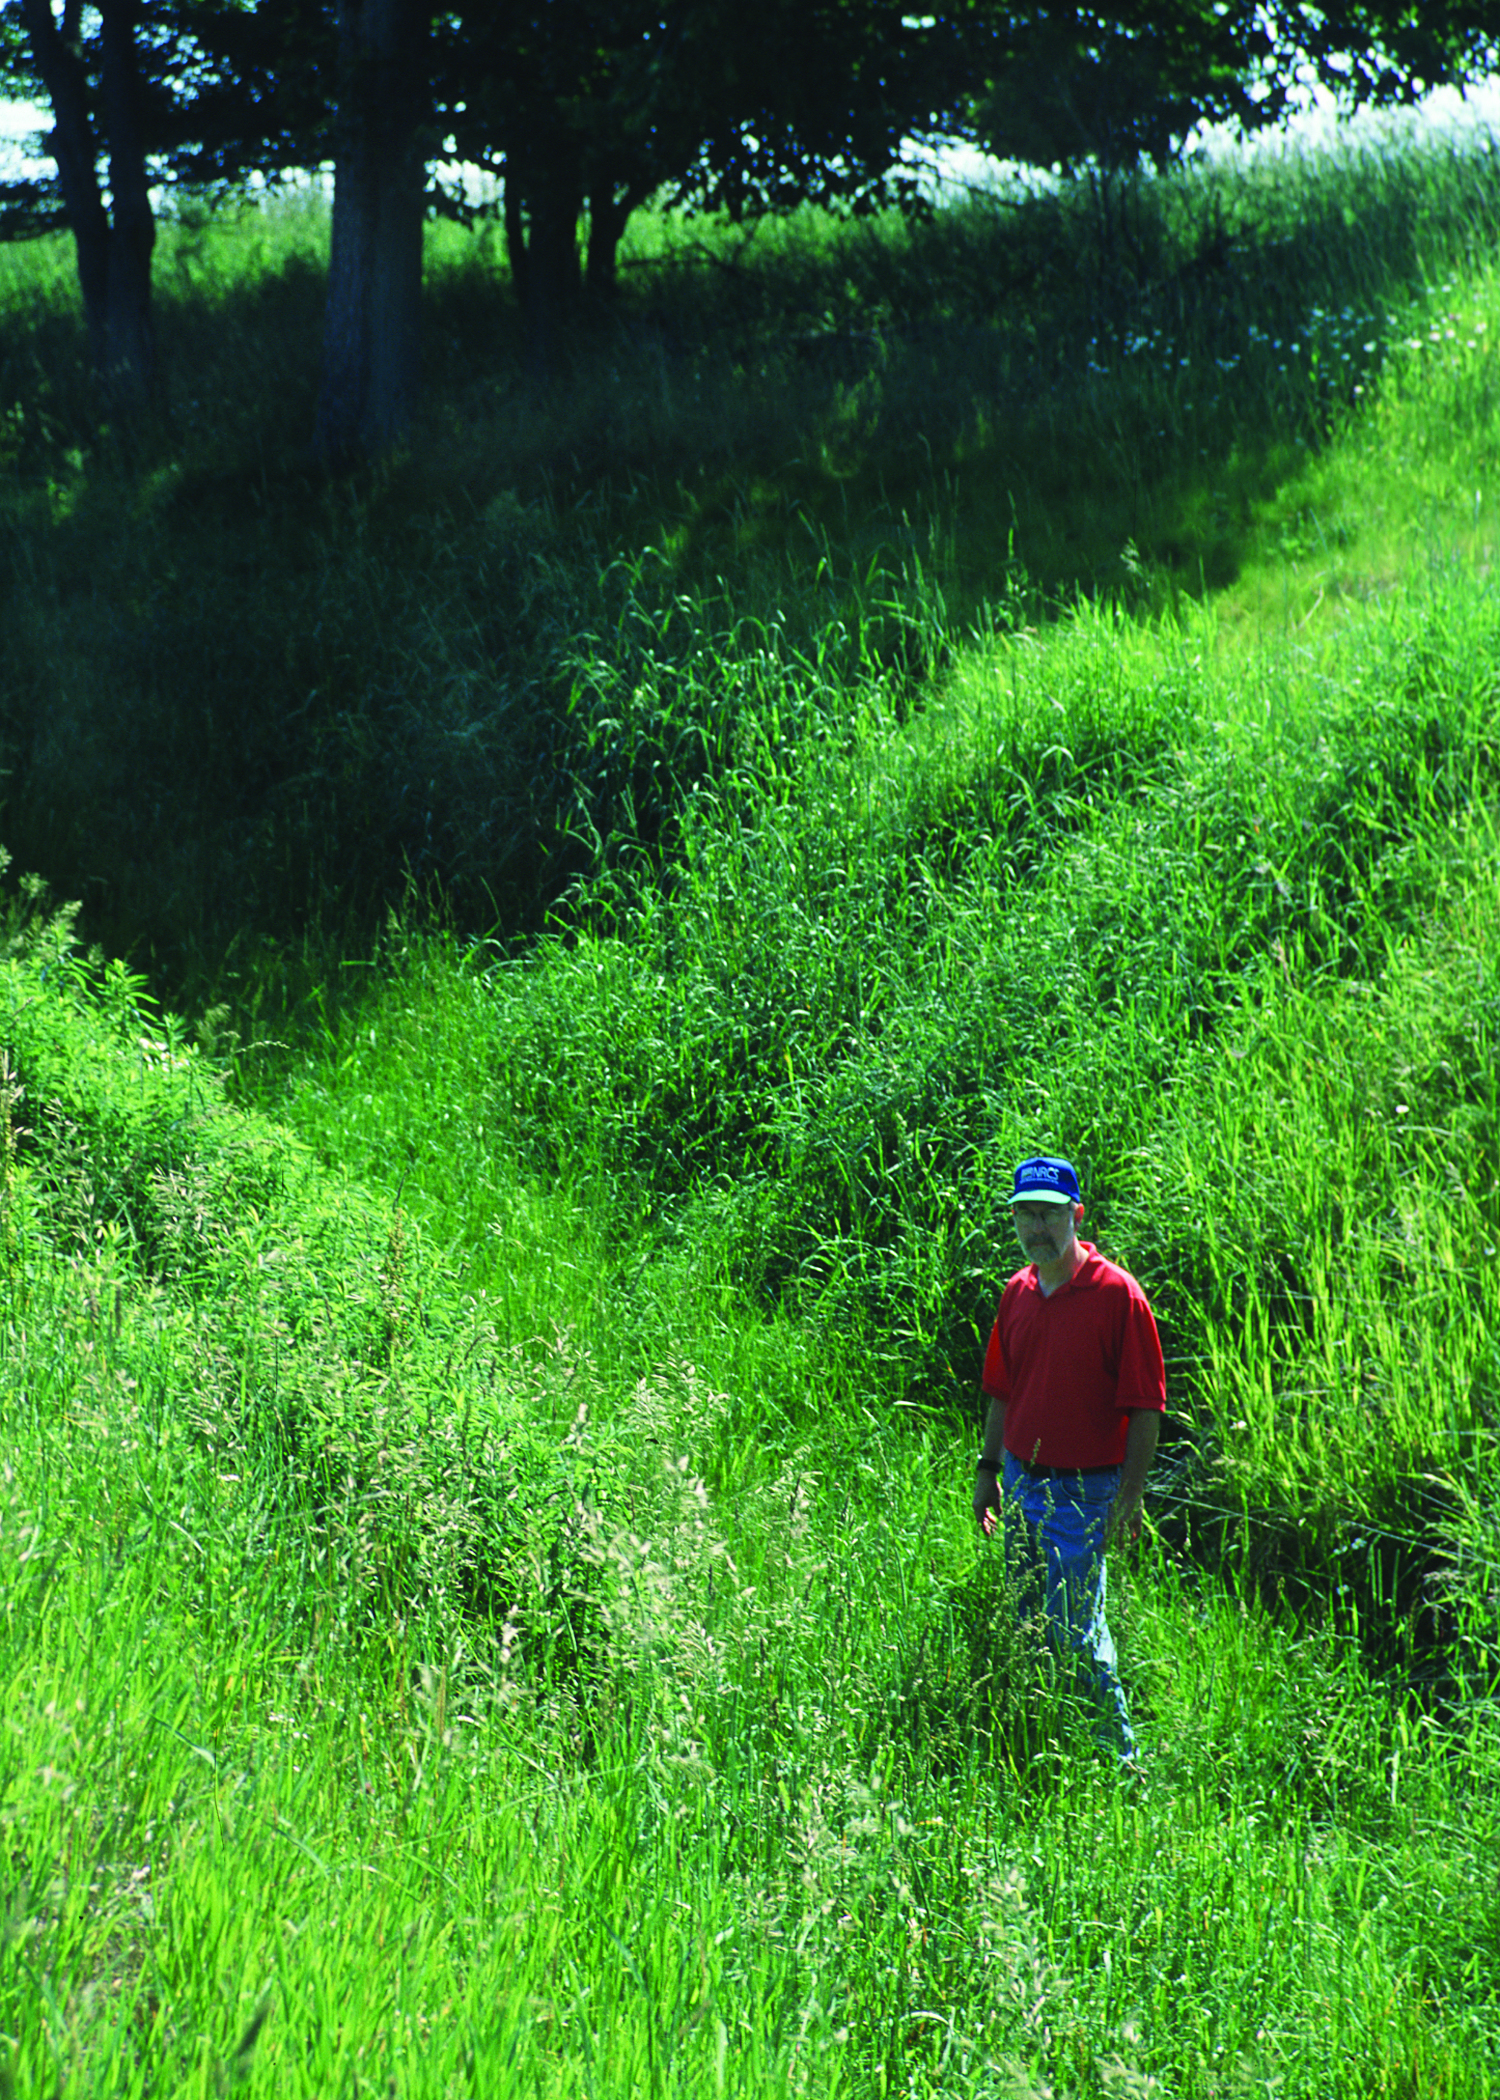
\includegraphics[keepaspectratio]{capitulos/../img/geotextil_talude.jpg}}

}

\caption{\label{fig-biomanta-talude}Biomanta instalada em talude ---
proteção imediata contra erosão enquanto a vegetação se estabelece.}

\end{figure}%

\end{minipage}%
%
\begin{minipage}{0.50\linewidth}

\begin{figure}[H]

\centering{

\pandocbounded{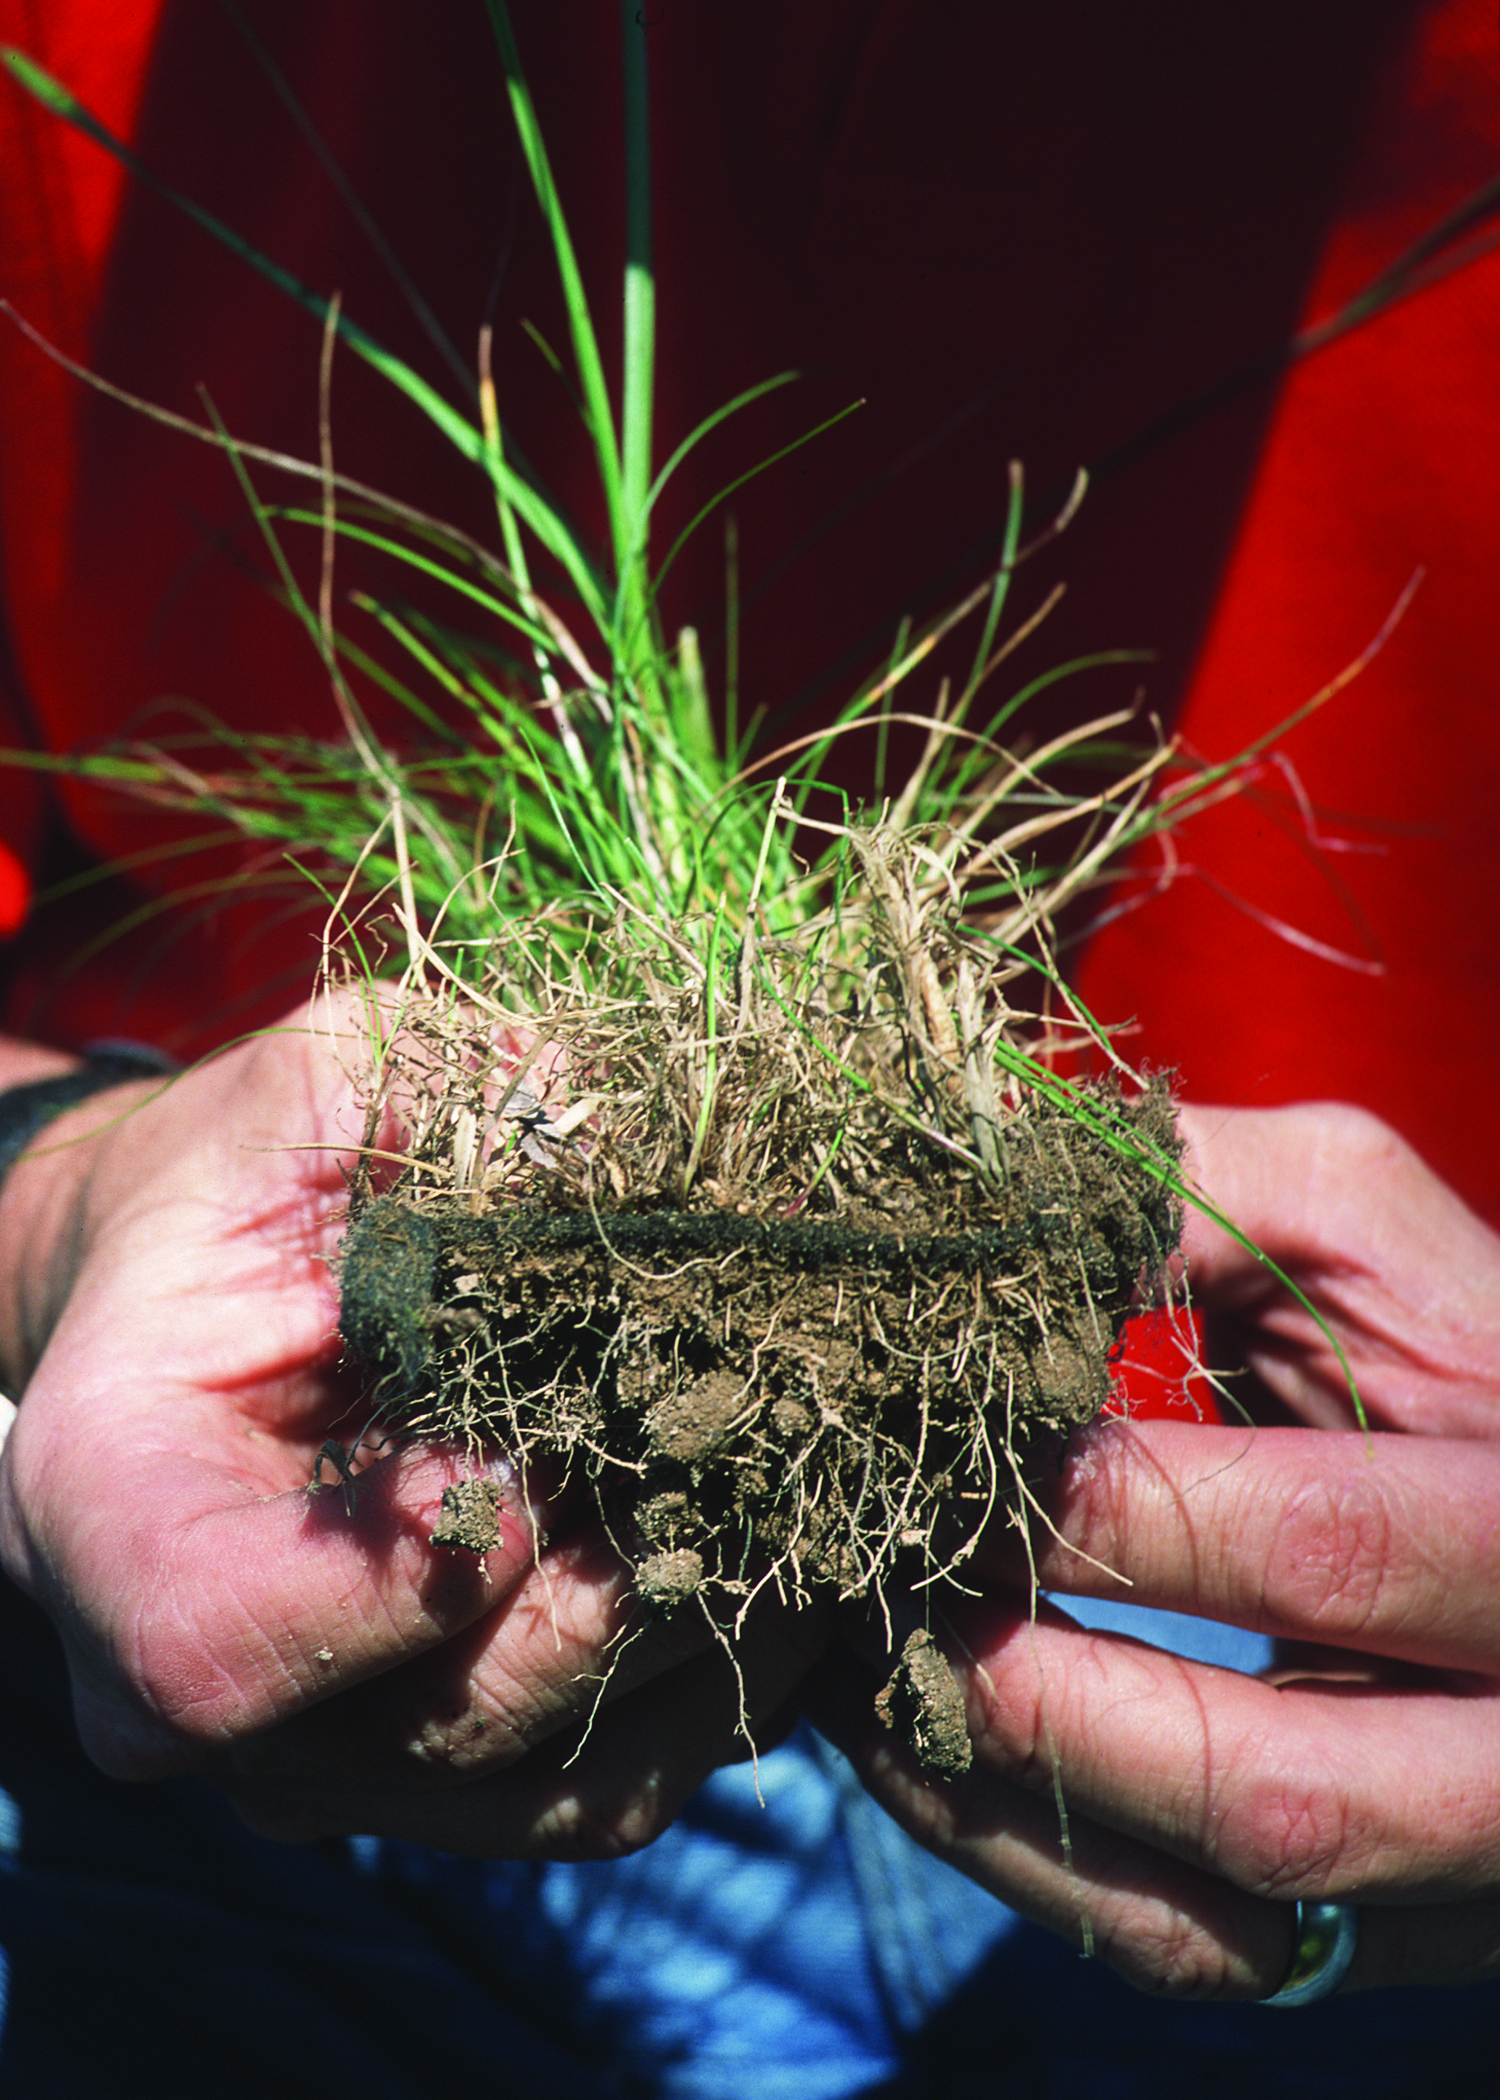
\includegraphics[keepaspectratio]{capitulos/../img/biomanta_grama.jpg}}

}

\caption{\label{fig-biomanta-grama}Vegetação emergindo através da
biomanta --- a grama se estabelece através das aberturas da manta.}

\end{figure}%

\end{minipage}%

\end{figure}%

\section{Classificação}\label{classificauxe7uxe3o}

\subsection{Por Material}\label{por-material}

A escolha do tipo de biomanta depende da durabilidade requerida pelo
projeto (que por sua vez depende do tempo necessário para a vegetação se
consolidar), do regime pluviométrico, da declividade do talude e do
orçamento disponível. A Tabela~\ref{tbl-biomantas} sintetiza as cinco
categorias comerciais mais utilizadas no Brasil.

\begin{longtable}[]{@{}
  >{\raggedright\arraybackslash}p{(\linewidth - 6\tabcolsep) * \real{0.1304}}
  >{\raggedright\arraybackslash}p{(\linewidth - 6\tabcolsep) * \real{0.3478}}
  >{\raggedright\arraybackslash}p{(\linewidth - 6\tabcolsep) * \real{0.2826}}
  >{\raggedright\arraybackslash}p{(\linewidth - 6\tabcolsep) * \real{0.2391}}@{}}
\caption{Tipos de biomantas e suas
características.}\label{tbl-biomantas}\tabularnewline
\toprule\noalign{}
\begin{minipage}[b]{\linewidth}\raggedright
Tipo
\end{minipage} & \begin{minipage}[b]{\linewidth}\raggedright
Fibra principal
\end{minipage} & \begin{minipage}[b]{\linewidth}\raggedright
Durabilidade
\end{minipage} & \begin{minipage}[b]{\linewidth}\raggedright
Aplicação preferencial
\end{minipage} \\
\midrule\noalign{}
\endfirsthead
\toprule\noalign{}
\begin{minipage}[b]{\linewidth}\raggedright
Tipo
\end{minipage} & \begin{minipage}[b]{\linewidth}\raggedright
Fibra principal
\end{minipage} & \begin{minipage}[b]{\linewidth}\raggedright
Durabilidade
\end{minipage} & \begin{minipage}[b]{\linewidth}\raggedright
Aplicação preferencial
\end{minipage} \\
\midrule\noalign{}
\endhead
\bottomrule\noalign{}
\endlastfoot
Biomanta de coco & Coco (\emph{Cocos nucifera}) & 2--4 anos & Taludes
rodoviários, margens fluviais \\
Biomanta de juta & Juta (\emph{Corchorus} spp.) & 1--2 anos & Canais,
áreas planas com chuva moderada \\
Biomanta de palha & Palha de arroz/trigo & 6--12 meses & Proteção
temporária de obras em andamento \\
Biomanta de sisal & Sisal (\emph{Agave sisalana}) & 2--5 anos & Taludes
íngremes (\textgreater{} 45°) \\
Biomanta mista & Coco + palha & 1--3 anos & Uso geral (melhor
custo-benefício) \\
\end{longtable}

A biomanta de coco é a mais versátil e robusta para condições tropicais
brasileiras, combinando alta resistência mecânica das fibras de
mesocarpo do coco (1 m de comprimento, Ø 0,1--0,3 mm) com excelente
retenção hídrica e degradação lenta (2--4 anos), que coincide com o
tempo necessário para a vegetação atingir plena maturidade radicular em
solos tropicais.

\subsection{Por Função (Norma ABNT NBR
16308)}\label{por-funuxe7uxe3o-norma-abnt-nbr-16308}

A norma ABNT NBR 16308 classifica as biomantas em quatro classes
funcionais que orientam a especificação técnica em projetos de
engenharia. A Classe I destina-se à proteção temporária (até 12 meses),
adequada para canteiros de obras ou áreas onde a revegetação é rápida. A
Classe II provê proteção de curta duração (12--24 meses), indicada para
taludes com declividade moderada (\textless{} 30°) em clima úmido. A
Classe III oferece proteção de média duração (24--48 meses), recomendada
para taludes íngremes ou áreas com revegetação lenta (solos arenosos,
clima semiárido). A Classe IV garante proteção de longa duração
(\textgreater{} 48 meses), reservada para situações críticas como
margens fluviais com erosão ativa ou taludes de barragens.

\section{Propriedades Mecânicas}\label{propriedades-mecuxe2nicas}

A especificação técnica de biomantas exige a comparação de propriedades
mecânicas e hidráulicas entre os materiais disponíveis. A
Tabela~\ref{tbl-propriedades} apresenta essa comparação para as duas
biomantas mais utilizadas (coco e juta) e, como referência, para o
geotêxtil sintético de polipropileno que constitui a alternativa
convencional.

\begin{longtable}[]{@{}
  >{\raggedright\arraybackslash}p{(\linewidth - 6\tabcolsep) * \real{0.1912}}
  >{\raggedright\arraybackslash}p{(\linewidth - 6\tabcolsep) * \real{0.2500}}
  >{\raggedright\arraybackslash}p{(\linewidth - 6\tabcolsep) * \real{0.2500}}
  >{\raggedright\arraybackslash}p{(\linewidth - 6\tabcolsep) * \real{0.3088}}@{}}
\caption{Propriedades mecânicas
comparativas.}\label{tbl-propriedades}\tabularnewline
\toprule\noalign{}
\begin{minipage}[b]{\linewidth}\raggedright
Propriedade
\end{minipage} & \begin{minipage}[b]{\linewidth}\raggedright
Biomanta de coco
\end{minipage} & \begin{minipage}[b]{\linewidth}\raggedright
Biomanta de juta
\end{minipage} & \begin{minipage}[b]{\linewidth}\raggedright
Geotêxtil sintético
\end{minipage} \\
\midrule\noalign{}
\endfirsthead
\toprule\noalign{}
\begin{minipage}[b]{\linewidth}\raggedright
Propriedade
\end{minipage} & \begin{minipage}[b]{\linewidth}\raggedright
Biomanta de coco
\end{minipage} & \begin{minipage}[b]{\linewidth}\raggedright
Biomanta de juta
\end{minipage} & \begin{minipage}[b]{\linewidth}\raggedright
Geotêxtil sintético
\end{minipage} \\
\midrule\noalign{}
\endhead
\bottomrule\noalign{}
\endlastfoot
Massa por área & 400--900 g/m² & 300--600 g/m² & 100--400 g/m² \\
Resistência à tração & 2--8 kN/m & 1--4 kN/m & 5--50 kN/m \\
Retenção hídrica & Alta (8--10× peso seco) & Moderada (5--7× peso seco)
& Baixa (\textless{} 2× peso seco) \\
Permeabilidade & Alta & Alta & Variável (depende da gramatura) \\
Biodegradabilidade & Sim (2--4 anos) & Sim (1--2 anos) & Não
(\textgreater{} 100 anos) \\
\end{longtable}

A diferença mais relevante do ponto de vista da bioengenharia é a
retenção hídrica: enquanto o geotêxtil sintético praticamente não retém
água (funcionando apenas como filtro), a biomanta de coco absorve 8--10×
seu peso em água, criando um reservatório superficial que libera umidade
gradualmente para as sementes em germinação, efeito particularmente
valioso em regiões com períodos secos intermitentes.

\section{Instalação}\label{instalauxe7uxe3o-1}

A instalação correta da biomanta é tão importante quanto a escolha do
material. Falhas de instalação (especialmente bolsões de ar e ancoragem
insuficiente) são responsáveis por mais de 60\% dos casos de insucesso
relatados na literatura técnica.

\subsection{Preparação do Terreno}\label{preparauxe7uxe3o-do-terreno}

A superfície do talude deve ser previamente regularizada, removendo-se
torrões, pedras soltas e saliências que impediriam o contato íntimo
entre a manta e o solo. Após a regularização, aplicam-se fertilizante
(NPK 10-10-10 a 200--400 kg/ha) e sementes (conforme mistura definida no
projeto de revegetação, ver \textbf{?@sec-hidrossemeadura}) diretamente
sobre o solo antes da instalação da biomanta, de modo que a manta
funcione como cobertura protetora das sementes já distribuídas. Em
seguida, escava-se a trincheira de ancoragem no topo do talude, com
dimensões mínimas de 15×15 cm, onde a borda superior da biomanta será
enterrada.

\subsection{Fixação}\label{fixauxe7uxe3o}

A biomanta é ancorada na trincheira superior com grampos em U (mínimo 3
grampos por metro linear de trincheira) e desenrolada de cima para baixo
ao longo do talude, em sentido perpendicular às curvas de nível. A
fixação ao solo é feita com grampos metálicos distribuídos a cada
0,5--1,0 m em padrão alternado (trebolillo), garantindo que a manta
permaneça em contato direto com o solo mesmo sob a ação do vento e do
escoamento. A sobreposição entre faixas adjacentes deve ser de pelo
menos 10 cm (15 cm em taludes \textgreater{} 45°), com a faixa superior
sobrepondo a inferior (como telhas), evitando que o escoamento penetre
sob a manta na junta. O procedimento finaliza com a ancoragem da borda
inferior da biomanta em uma segunda trincheira na base do talude.

\subsection{Grampeamento}\label{grampeamento}

Os grampos são o elemento de fixação que garante a aderência da biomanta
ao solo sob as forças de arraste do escoamento e do vento. Utilizam-se
grampos em U de aço CA-25 (Ø 5 mm, comprimento 20--30 cm), cravados no
solo com martelo ou marreta. A densidade de grampeamento é de 2--4
grampos/m² em taludes inferiores a 45° e de 4--8 grampos/m² em taludes
superiores a 45°, valores que devem ser aumentados em 50\% nas zonas de
maior concentração de escoamento (concavidades, confluências de
micro-talvegues) e nas bordas laterais da biomanta.

\begin{tcolorbox}[enhanced jigsaw, leftrule=.75mm, colframe=quarto-callout-important-color-frame, colback=white, bottomrule=.15mm, opacityback=0, colbacktitle=quarto-callout-important-color!10!white, breakable, bottomtitle=1mm, opacitybacktitle=0.6, title=\textcolor{quarto-callout-important-color}{\faExclamation}\hspace{0.5em}{Ponto crítico}, titlerule=0mm, toprule=.15mm, toptitle=1mm, rightrule=.15mm, left=2mm, arc=.35mm, coltitle=black]

O contato íntimo entre a biomanta e o solo é essencial para o sucesso da
técnica. Bolsões de ar sob a manta criam caminhos preferenciais de
escoamento que concentram o fluxo (fenômeno análogo ao \emph{piping}),
gerando erosão subsuperficial localizada que pode destruir toda a
instalação em um único evento chuvoso intenso. A principal medida
preventiva é a regularização cuidadosa da superfície antes da instalação
e o grampeamento em densidade adequada, particularmente nas concavidades
do terreno.

\end{tcolorbox}

\section{Vantagens sobre Geossintéticos
Convencionais}\label{vantagens-sobre-geossintuxe9ticos-convencionais}

As biomantas oferecem cinco vantagens técnicas e ambientais em relação
aos geossintéticos sintéticos (polipropileno, poliéster). A
biodegradabilidade garante que não haverá resíduos plásticos permanentes
no solo após o cumprimento da função de proteção, evitando a
contaminação por microplásticos que ocorre com a fragmentação de
geotêxteis sintéticos. A incorporação de matéria orgânica ao solo
durante a degradação (1--4 t C/ha) melhora a estrutura, a retenção
hídrica e a atividade biológica do substrato. A retenção hídrica das
fibras naturais é 3--5× superior à dos sintéticos, favorecendo a
germinação em períodos secos. A rugosidade superficial elevada das
fibras de coco e juta reduz a velocidade do escoamento em 40--60\% em
comparação com geotêxteis de polipropileno de superfície lisa. O custo é
tipicamente 30--50\% inferior ao dos geossintéticos de polipropileno de
gramatura equivalente.

\section{Custos}\label{custos-2}

A Tabela~\ref{tbl-custos-biomanta} apresenta a composição de custos por
metro quadrado para a biomanta de coco (700 g/m²), que é a especificação
mais comum em projetos de bioengenharia no Brasil.

\begin{longtable}[]{@{}ll@{}}
\caption{Custo médio de implantação de biomanta de
coco.}\label{tbl-custos-biomanta}\tabularnewline
\toprule\noalign{}
Item & Valor (R\$/m²) \\
\midrule\noalign{}
\endfirsthead
\toprule\noalign{}
Item & Valor (R\$/m²) \\
\midrule\noalign{}
\endhead
\bottomrule\noalign{}
\endlastfoot
Biomanta de coco (700 g/m²) & 8--15 \\
Grampos (4/m²) & 2--4 \\
Mão de obra de instalação & 5--10 \\
Sementes + fertilizante pré-instalação & 3--6 \\
Total & 18--35 \\
\end{longtable}

O custo total de R\$ 18--35/m² compara-se aos R\$ 9--18/ha da
hidrossemeadura simples (ver \textbf{?@sec-hidrossemeadura}) e aos R\$
40--80/m² dos geotêxteis sintéticos com grampeamento. A biomanta é,
portanto, a solução intermediária em custo e proteção, indicada quando a
hidrossemeadura sozinha é insuficiente (taludes \textgreater{} 30° ou
solos muito erodíveis) mas o geotêxtil sintético é dispensável (ausência
de cargas estruturais permanentes).

\chapter{Enrocamento Vegetado}\label{enrocamento-vegetado}

\# Enrocamento Vegetado \{\#sec-enrocamento\}

O enrocamento vegetado (\emph{vegetated riprap}) combina a proteção
mecânica imediata de pedras com o reforço biológico progressivo
fornecido por plantas vivas inseridas entre as pedras. Trata-se de uma
técnica de bioengenharia para proteção de margens fluviais e bases de
taludes submetidos a fluxo d'água, onde a ação hidrodinâmica
(velocidade, turbulência, ondas) exige uma resistência mecânica que a
vegetação sozinha não pode oferecer nos primeiros anos, mas a solução
puramente inerte (enrocamento convencional) não proporciona os serviços
ecossistêmicos e a durabilidade de longo prazo que o sistema radicular
proporciona.

O princípio de funcionamento baseia-se na complementaridade temporal
entre dois mecanismos de proteção. Nos primeiros 3--5 anos após a
instalação, as pedras fornecem 100\% da resistência ao arraste e à
erosão, enquanto as estacas vivas inseridas entre elas enraízam, brotam
e desenvolvem progressivamente um sistema radicular que penetra 1--3 m
no solo subjacente. Após esse período de transição, as raízes criam uma
ancoragem biológica que complementa e paulatinamente substitui a função
mecânica das pedras, de modo que eventuais deslocamentos de pedras
individuais não comprometem a estabilidade do conjunto. A
Figura~\ref{fig-riprap-rio} mostra um enrocamento convencional em margem
fluvial, onde as pedras protegem a base contra a erosão do fluxo,
enquanto a Figura~\ref{fig-riprap-vegetado} apresenta um enrocamento
vegetado em estágio avançado de consolidação biológica, com a vegetação
já plenamente estabelecida entre as pedras.

\begin{figure}

\begin{minipage}{0.50\linewidth}

\begin{figure}[H]

\centering{

\pandocbounded{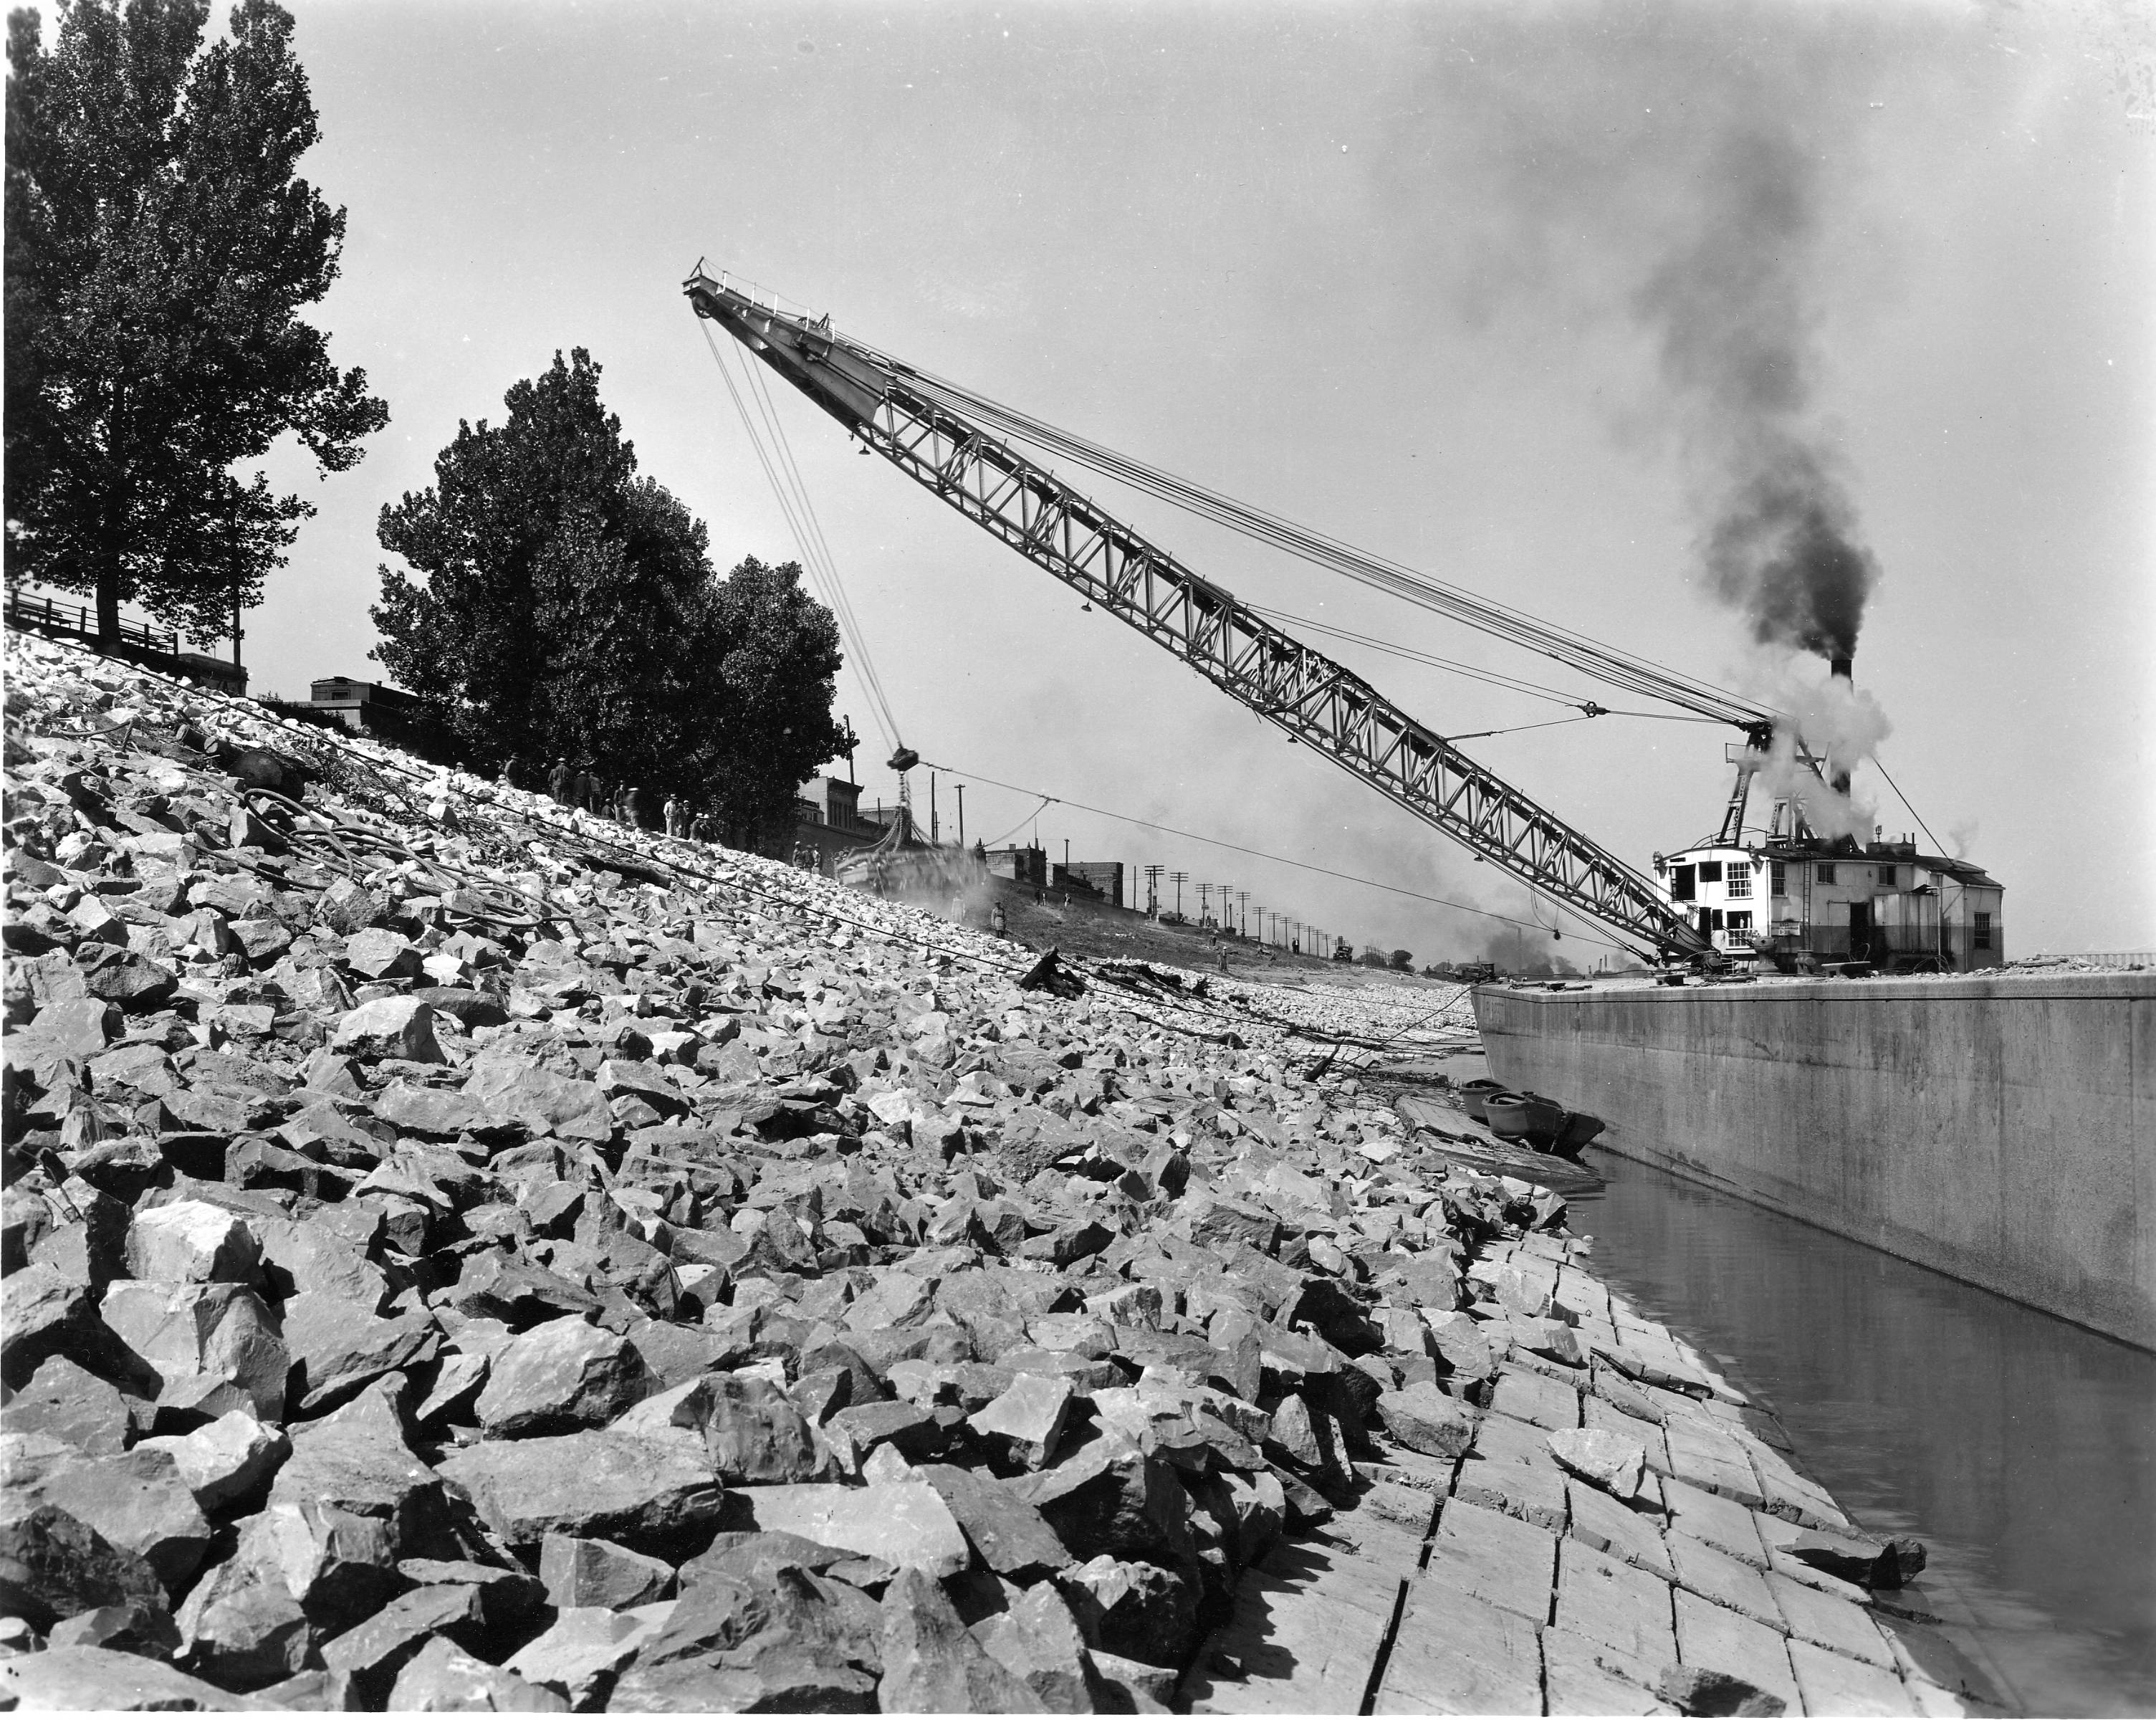
\includegraphics[keepaspectratio]{capitulos/../img/riprap_rio.jpg}}

}

\caption{\label{fig-riprap-rio}Enrocamento em margem fluvial --- pedras
protegem a base enquanto a vegetação se estabelece entre os
interstícios.}

\end{figure}%

\end{minipage}%
%
\begin{minipage}{0.50\linewidth}

\begin{figure}[H]

\centering{

\pandocbounded{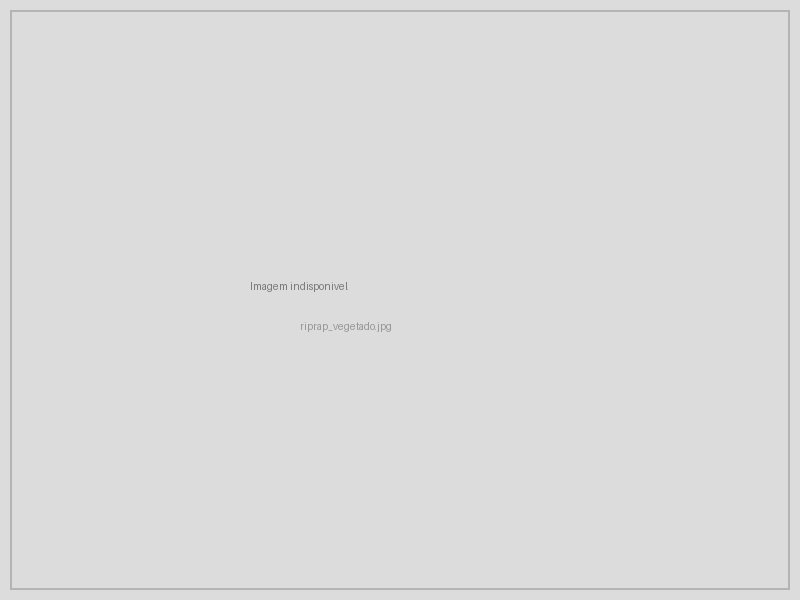
\includegraphics[keepaspectratio]{capitulos/../img/riprap_vegetado.jpg}}

}

\caption{\label{fig-riprap-vegetado}Enrocamento vegetado --- combinação
de proteção mecânica e biológica em estágio avançado de consolidação.}

\end{figure}%

\end{minipage}%

\end{figure}%

\section{Componentes}\label{componentes}

O enrocamento vegetado é composto por três elementos estruturais. As
pedras devem ter diâmetro médio entre 15 e 50 cm e massa individual
entre 5 e 150 kg, privilegiando-se rochas compactas, densas e
resistentes à abrasão (granito, gnaisse, basalto), evitando-se rochas
friáveis (xisto, arenito mal cimentado) que se fragmentam sob impacto.
As estacas vivas são ramos ou troncos jovens de espécies com elevada
capacidade de enraizamento vegetativo, inseridos entre as pedras durante
a construção, com diâmetro de 3--8 cm e comprimento suficiente para
transpor toda a espessura do enrocamento e penetrar no solo subjacente.
A camada de filtro é o elemento mais frequentemente negligenciado em
projetos mal executados, consistindo em geotêxtil não-tecido ou camada
de transição granulométrica posicionada entre o solo natural e as
pedras, cuja função é impedir a remoção seletiva de partículas finas do
solo pelo fluxo d'água (\emph{suffusion}), que é a principal causa de
colapso de enrocamentos pela perda de suporte da fundação.

\section{Dimensionamento das Pedras}\label{dimensionamento-das-pedras}

O diâmetro médio das pedras (\(D_{50}\)) é a variável de projeto mais
importante e é calculado em função da velocidade do fluxo a que a margem
está submetida, utilizando a equação de Isbash adaptada

\[
D_{50} = \frac{0{,}06 \cdot V^2}{(\gamma_s / \gamma_w - 1) \cdot g}
\]

onde \(V\) é a velocidade do fluxo na margem (m/s), determinada por
medição em campo ou por modelagem hidráulica, \(\gamma_s\) é o peso
específico da pedra (tipicamente 26 kN/m³ para granito e basalto),
\(\gamma_w\) é o peso específico da água (9,81 kN/m³) e \(g\) é a
aceleração gravitacional (9,81 m/s²). O resultado dessa equação indica o
diâmetro mínimo da pedra que resiste ao arraste hidrodinâmico sem ser
mobilizada pelo fluxo.

\subsection{Espessura da Camada}\label{espessura-da-camada}

A espessura mínima do enrocamento (\(e\)) deve ser

\[
e = 1{,}5 \cdot D_{50}
\]

e nunca inferior a 30 cm, garantindo que as pedras se arranjem em pelo
menos duas camadas sobrepostas, criando intertravamento mecânico que
impede o deslocamento individual. Em margens submetidas a ondas de
embarcações ou variação rápida de nível d'água, a espessura deve ser
aumentada para \(2{,}0 \cdot D_{50}\).

\section{Vegetação no Enrocamento}\label{vegetauxe7uxe3o-no-enrocamento}

\subsection{Espécies Indicadas}\label{espuxe9cies-indicadas}

A seleção de espécies para vegetação do enrocamento deve priorizar a
capacidade de enraizamento em ambiente parcialmente submerso (zona de
variação do nível d'água), a tolerância a inundações periódicas e a
produção de raízes profundas e densas. As espécies mais indicadas para o
contexto brasileiro incluem \emph{Salix} spp. (salgueiro) em zonas
temperadas e subtropicais do Sul e Sudeste, com taxa de enraizamento
superior a 90\% e crescimento rápido (2--3 m/ano); \emph{Mimosa
caesalpiniifolia} (sabiá) na Caatinga e Tabuleiros Costeiros, com
madeira de alta durabilidade natural que resiste à degradação mesmo
quando parcialmente submersa; \emph{Gliricidia sepium} (gliricídia) em
regiões pantropicais, combinando excelente brotação com fixação
biológica de nitrogênio; \emph{Inga} spp. (ingá) em mata ciliar
tropical, espécie nativa que reconstitui a vegetação ripária original;
além de gramíneas rizomatosas (\emph{Paspalum}, \emph{Cynodon}) nos
interstícios superficiais, que proporcionam cobertura rápida e filtração
de sedimentos finos.

\subsection{Instalação}\label{instalauxe7uxe3o-2}

O procedimento de instalação é executado em camadas, iniciando com a
preparação da base do talude mediante colocação de filtro geotêxtil
não-tecido (gramatura mínima 200 g/m²) ou geotêxtil biodegradável de
coco (ver \textbf{?@sec-biomantas}) sobre o solo natural da margem.
Sobre o filtro, assenta-se a primeira camada de pedras, arranjadas com a
face mais plana voltada para baixo para maximizar o contato e o
intertravamento. As estacas vivas são então inseridas entre as pedras,
em ângulo de 15--20° com a horizontal (essa inclinação facilita o
enraizamento e direciona o crescimento da copa para fora da face do
enrocamento), com as pontas inferiores penetrando no solo subjacente e
as superiores projetando-se 20--30 cm além da face do enrocamento. Os
interstícios são preenchidos com solo vegetal (mistura de solo local com
20\% de composto orgânico). Camadas adicionais são completadas até a
cota de projeto, repetindo o procedimento de alternância
pedras--estacas--solo, finalizando com semeadura de gramíneas nos
interstícios superficiais.

\begin{tcolorbox}[enhanced jigsaw, leftrule=.75mm, colframe=quarto-callout-tip-color-frame, colback=white, bottomrule=.15mm, opacityback=0, colbacktitle=quarto-callout-tip-color!10!white, breakable, bottomtitle=1mm, opacitybacktitle=0.6, title=\textcolor{quarto-callout-tip-color}{\faLightbulb}\hspace{0.5em}{Transição funcional}, titlerule=0mm, toprule=.15mm, toptitle=1mm, rightrule=.15mm, left=2mm, arc=.35mm, coltitle=black]

Após 3--5 anos, as raízes das estacas vivas penetram 1--3 m no solo,
criando uma ancoragem biológica que complementa e gradualmente substitui
a função mecânica das pedras. O enrocamento evolui de uma estrutura
inerte para um ecossistema ripário funcional, com contribuições
ecossistêmicas adicionais como habitat para fauna aquática e terrestre,
filtração de nutrientes e sedimentos do escoamento lateral, estabilidade
térmica da água pela sombra da copa e sequestro de carbono na biomassa e
no solo.

\end{tcolorbox}

\section{Aplicações Típicas}\label{aplicauxe7uxf5es-tuxedpicas}

A Tabela~\ref{tbl-enrocamento} orienta o dimensionamento do enrocamento
em função da velocidade do fluxo para as situações mais comuns de
projeto, desde margens com erosão lenta até vertedouros de barragens.

\begin{longtable}[]{@{}llll@{}}
\caption{Dimensionamento de enrocamento por velocidade de
fluxo.}\label{tbl-enrocamento}\tabularnewline
\toprule\noalign{}
Situação & Velocidade do fluxo & D₅₀ recomendado & Espessura mínima \\
\midrule\noalign{}
\endfirsthead
\toprule\noalign{}
Situação & Velocidade do fluxo & D₅₀ recomendado & Espessura mínima \\
\midrule\noalign{}
\endhead
\bottomrule\noalign{}
\endlastfoot
Margens com erosão lenta & 1--2 m/s & 10--20 cm & 30 cm \\
Margens com erosão ativa & 2--3 m/s & 20--35 cm & 40--55 cm \\
Pilares de ponte & 3--4 m/s & 35--50 cm & 55--75 cm \\
Vertedouros de barragens & \textgreater{} 4 m/s & \textgreater{} 50 cm &
\textgreater{} 75 cm \\
\end{longtable}

\section{Custos}\label{custos-3}

O enrocamento simples (sem vegetação) custa entre R\$ 80 e R\$ 150/m²,
incluindo pedras, filtro geotêxtil, transporte e mão de obra. O
enrocamento vegetado situa-se entre R\$ 100 e R\$ 200/m², com o
acréscimo correspondendo às estacas vivas, ao solo vegetal, ao composto
orgânico e à semeadura de gramíneas. Para comparação, o muro de gabião
(ver \textbf{?@sec-gabiao-vivo}) varia de R\$ 200 a R\$ 400/m² e o muro
de concreto armado de R\$ 800 a R\$ 1.500/m².

O sobrecusto da vegetação (20--30\% sobre o enrocamento simples) é
justificado pela durabilidade ampliada da obra (as raízes compensam a
perda de intertravamento por deslocamento de pedras), pelos serviços
ecossistêmicos adicionais (habitat, filtração, paisagem, carbono) e pela
redução de custos de manutenção a longo prazo, uma vez que o enrocamento
vegetado consolidado dispensa as intervenções periódicas de reposição de
pedras que o enrocamento convencional frequentemente exige após cheias
excepcionais.

\chapter{Cordões Vegetativos}\label{corduxf5es-vegetativos}

\# Cordões Vegetativos e Fascinas \{\#sec-cordoes-fascinas\}

\subsection{Cordões Vegetativos}\label{corduxf5es-vegetativos-1}

Os cordões vegetativos são faixas de vegetação densa (1--3 m de largura)
dispostas ao longo de curvas de nível em encostas, formando barreiras
biológicas contínuas ao escoamento superficial laminar. Diferentemente
dos feixes vivos (ver \textbf{?@sec-feixes-drenos}), que são estruturas
construídas com ramos amarrados em valas, os cordões vegetativos são
faixas plantadas de espécies perenes que, após o estabelecimento, formam
uma barreira viva permanente, autossustentável e de manutenção mínima.

O mecanismo de funcionamento opera em duas escalas. Em escala
superficial, a vegetação densa reduz a velocidade do escoamento laminar
por aumento da rugosidade hidráulica, promovendo a deposição dos
sedimentos transportados a montante do cordão. Ao longo dos anos, essa
deposição acumula uma camada de solo que eleva progressivamente o nível
do terreno a montante, criando terraços naturais (fenômeno denominado
\emph{sediment wedge}) que suavizam a declividade original da encosta.
Em escala subsuperficial, o sistema radicular profundo e denso das
espécies utilizadas (particularmente o vetiver, com raízes de até 4 m)
aumenta a coesão do solo e a resistência ao cisalhamento, reduzindo a
suscetibilidade a deslizamentos rasos. A Figura~\ref{fig-cordao} mostra
a construção de um cordão vegetativo por entrelaçamento de ramos,
evidenciando a técnica de implantação que combina elementos vivos e
mortos para obter barreira funcional desde o primeiro dia.

\begin{figure}

\centering{

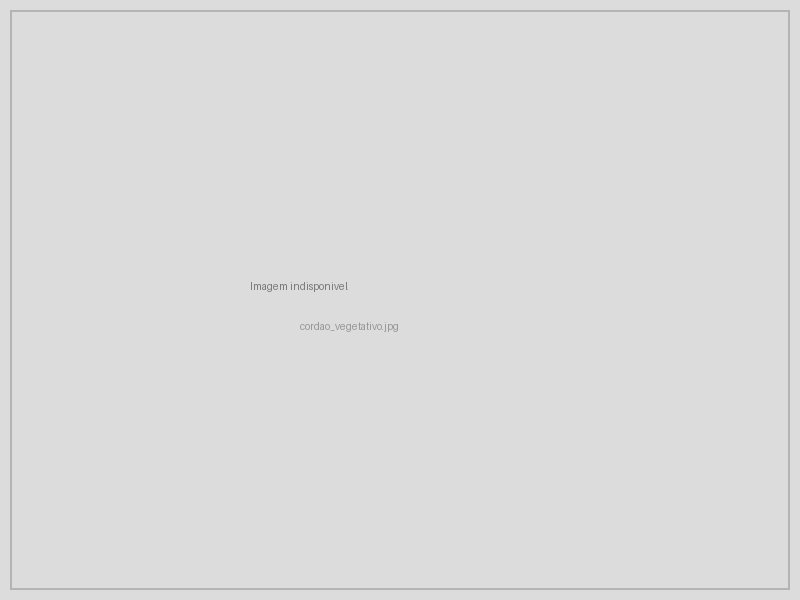
\includegraphics[width=0.8\linewidth,height=\textheight,keepaspectratio]{capitulos/../img/cordao_vegetativo.jpg}

}

\caption{\label{fig-cordao}Construção de cordão vegetativo com
entrelaçamento de ramos --- barreira biológica que retarda o escoamento
superficial.}

\end{figure}%

Técnicas complementares de estabilização biológica são também utilizadas
em contextos semelhantes. A Figura~\ref{fig-fascina} apresenta uma cerca
de fascina construída com salgueiro, estrutura biodegradável que
estabiliza taludes por entrelaçamento de ramos vivos, enquanto a
Figura~\ref{fig-barreira} mostra uma barreira de salgueiro em estágio
avançado, com as estacas já brotando e formando um cordão vegetativo
consolidado.

\begin{figure}

\begin{minipage}{0.50\linewidth}

\begin{figure}[H]

\centering{

\pandocbounded{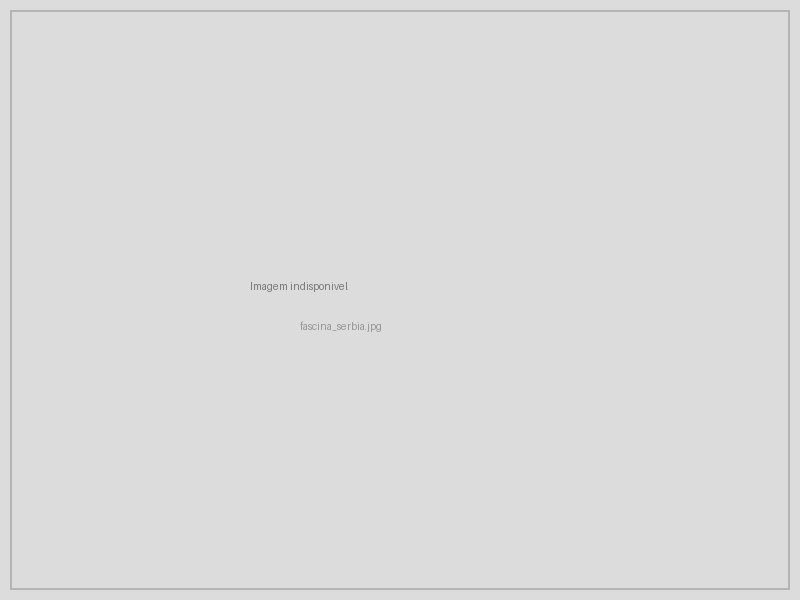
\includegraphics[keepaspectratio]{capitulos/../img/fascina_serbia.jpg}}

}

\caption{\label{fig-fascina}Cerca de fascina com salgueiro --- estrutura
biodegradável que estabiliza taludes por entrelaçamento de ramos.}

\end{figure}%

\end{minipage}%
%
\begin{minipage}{0.50\linewidth}

\begin{figure}[H]

\centering{

\pandocbounded{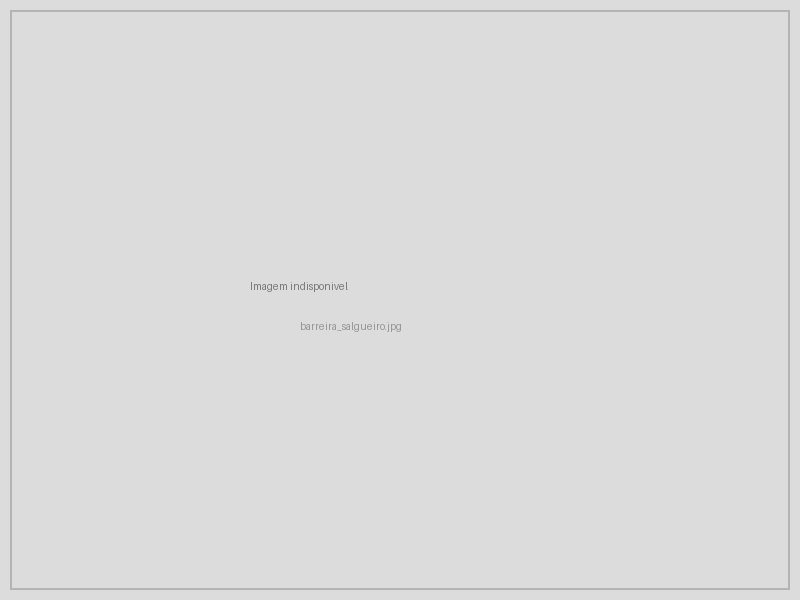
\includegraphics[keepaspectratio]{capitulos/../img/barreira_salgueiro.jpg}}

}

\caption{\label{fig-barreira}Barreira de salgueiro --- cordão vegetativo
em estágio avançado com brotamento das estacas.}

\end{figure}%

\end{minipage}%

\end{figure}%

\subsection{Espécies}\label{espuxe9cies}

A seleção da espécie é determinante para o sucesso do cordão vegetativo,
devendo-se considerar a profundidade e a densidade do sistema radicular,
a capacidade de formar barreira densa e impenetrável pelo fluxo, a
tolerância a condições edáficas extremas e a facilidade de propagação. A
Figura~\ref{fig-vetiver} demonstra o sistema radicular excepcionalmente
profundo e denso do vetiver em análise de campo, onde se observam raízes
que penetram até 4 m de profundidade, conferindo ancoragem e coesão ao
maciço de solo.

\begin{figure}

\centering{

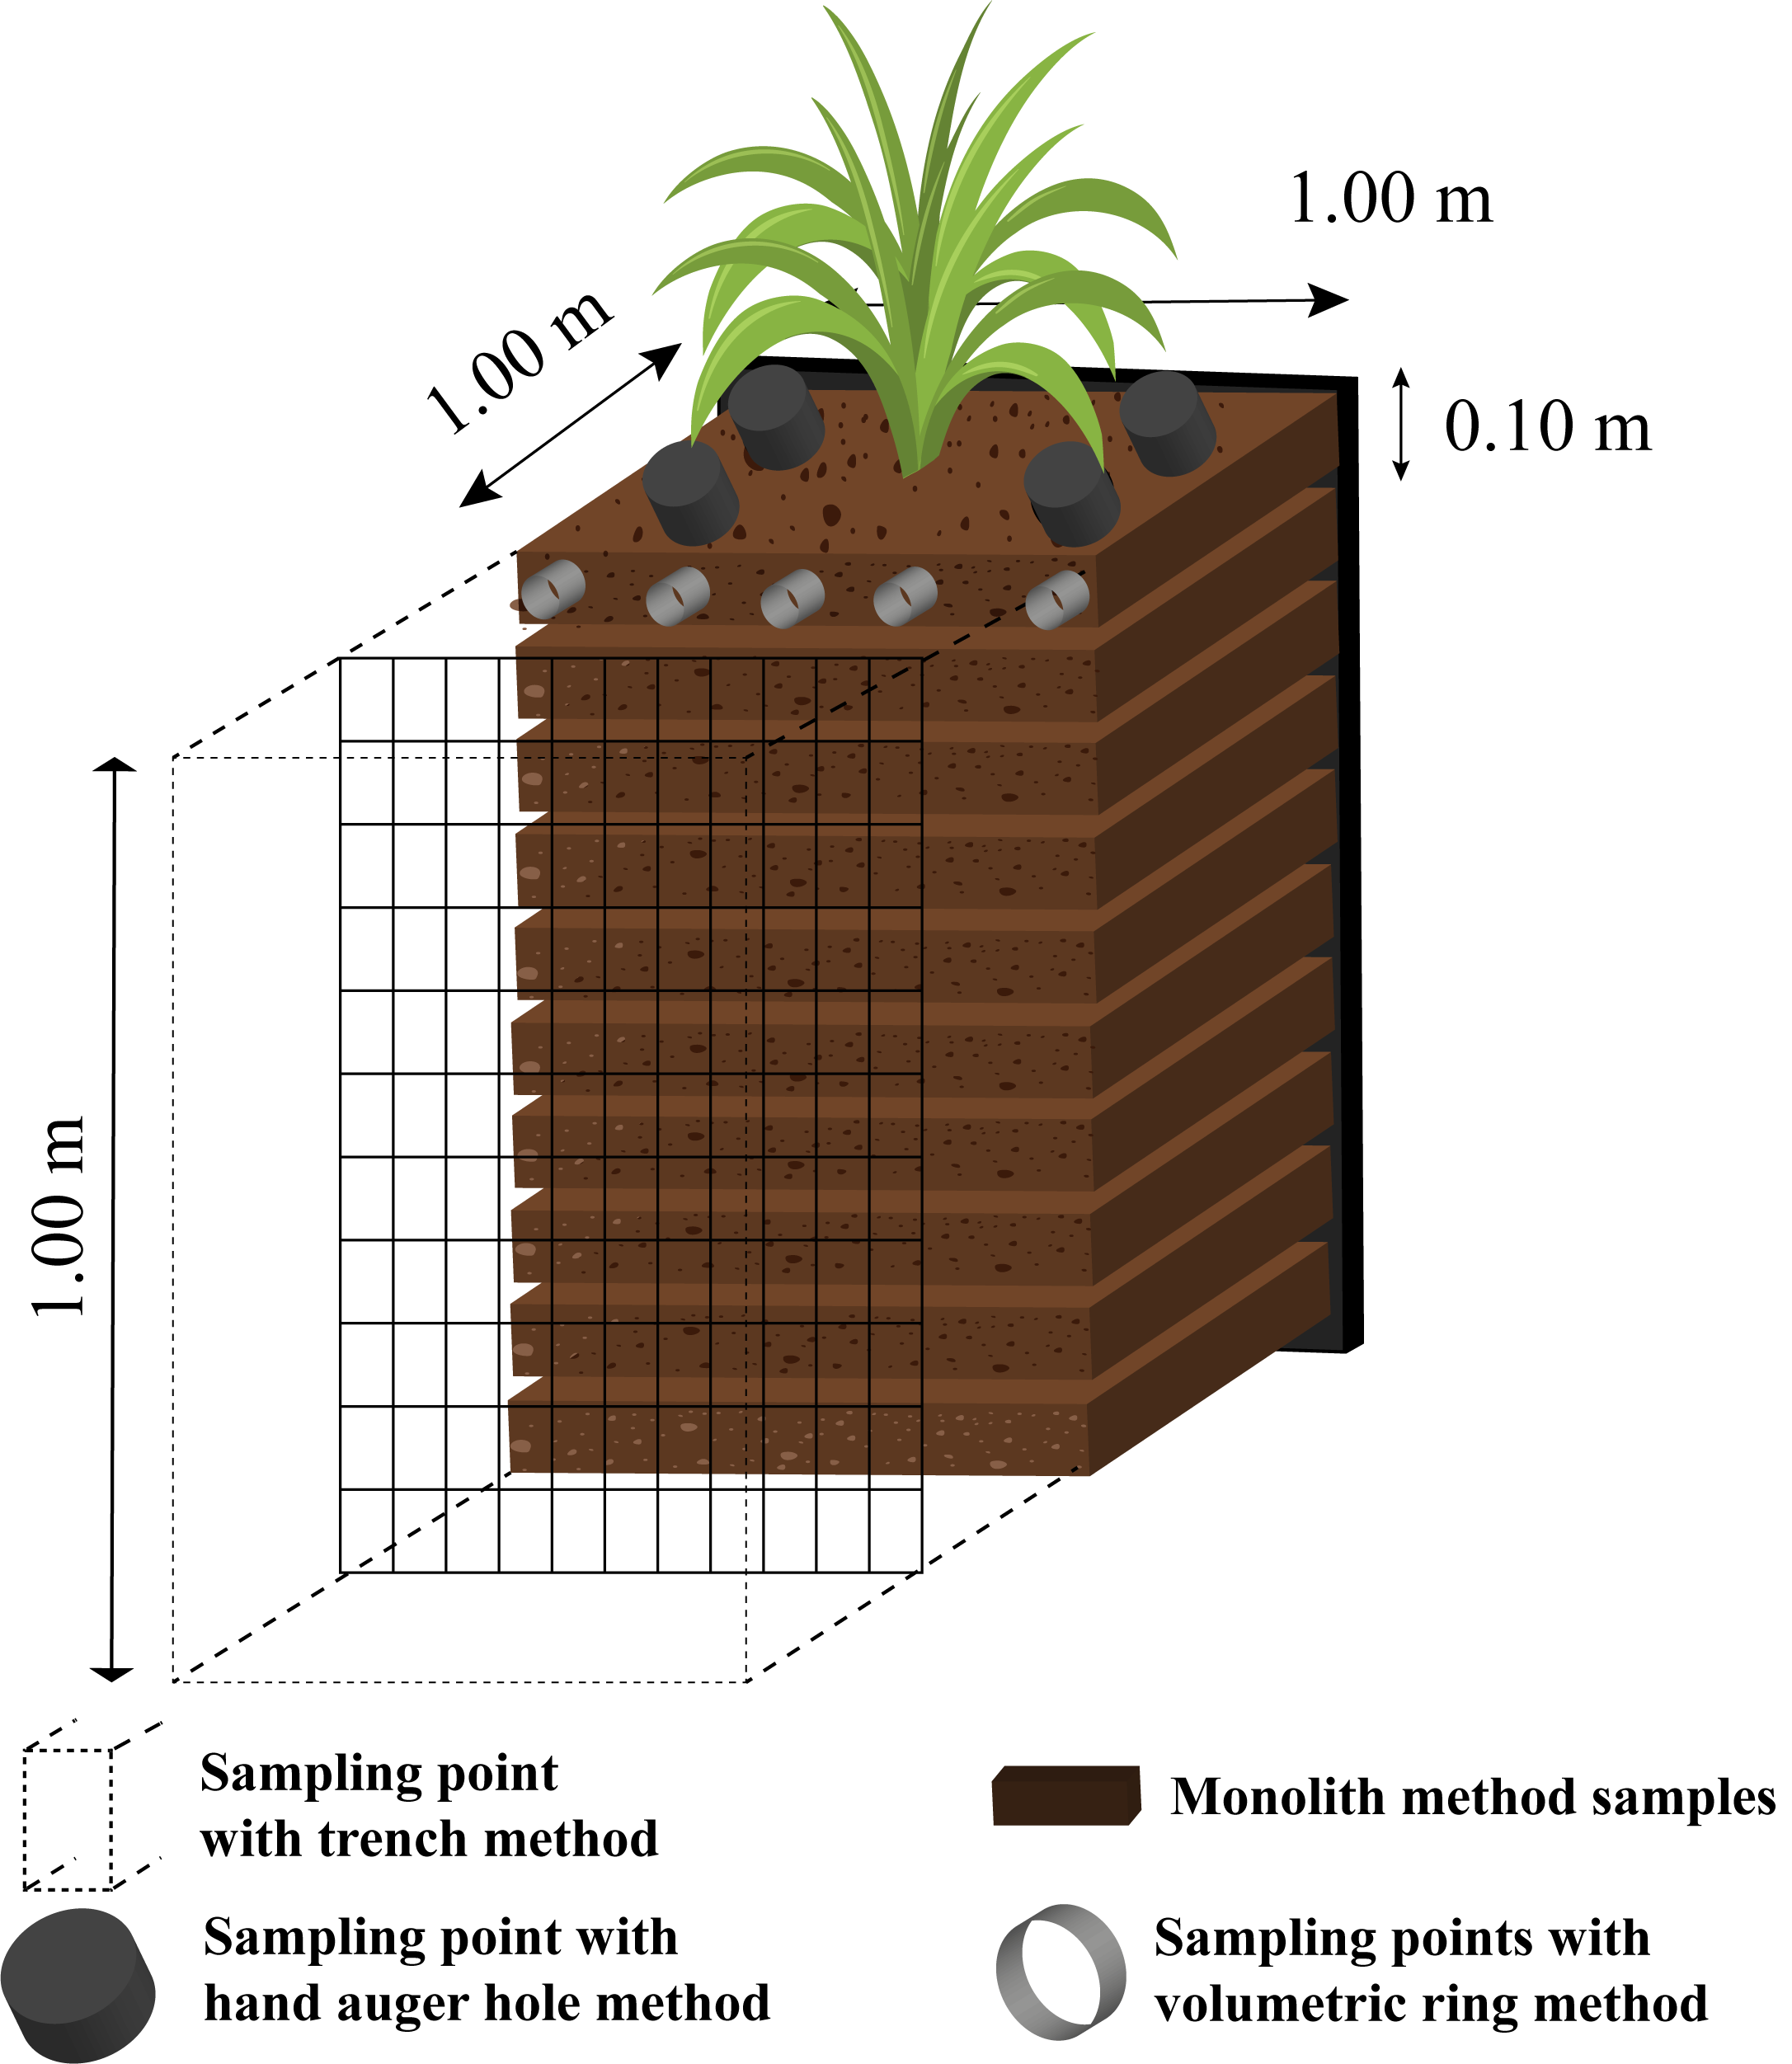
\includegraphics[width=0.8\linewidth,height=\textheight,keepaspectratio]{capitulos/../img/vetiver_analise.png}

}

\caption{\label{fig-vetiver}Análise de campo do sistema radicular de
vetiver --- raízes profundas (até 4 m) que conferem alta resistência à
tração.}

\end{figure}%

A espécie mais utilizada mundialmente para cordões vegetativos é o
vetiver (\emph{Vetiveria zizanioides}), que reúne características
excepcionais para a bioengenharia: sistema radicular vertical e profundo
(até 4 m), com raízes individuais de resistência à tração de 40--120 MPa
(comparável à de aços estruturais de baixa resistência); formação de
barreira densa e impenetrável pelo fluxo a partir de 4--6 meses após o
plantio; e extrema tolerância a condições adversas, suportando pH de 3 a
11, seca prolongada, encharcamento temporário, salinidade e metais
pesados.

Outras opções tropicais incluem o capim-elefante (\emph{Pennisetum
purpureum}), que produz biomassa abundante e pode ser utilizado como
forrageira; a cana-de-açúcar em curvas de nível, tradicional em áreas de
produção familiar; e a citronela (\emph{Cymbopogon nardus}), que
adiciona a propriedade repelente de insetos.

\subsection{Dimensionamento}\label{dimensionamento-4}

O dimensionamento de cordões vegetativos envolve dois parâmetros
principais. O espaçamento vertical entre cordões deve ser de 1--2 m de
desnível, com intervalos menores (1 m) em solos de alta erodibilidade e
maiores (2 m) em solos mais estáveis. A largura da faixa plantada deve
ser de 1--3 m, sendo que faixas mais largas oferecem maior capacidade de
filtração e retenção, porém ocupam mais área produtiva. O espaçamento
horizontal resultante entre cordões na encosta é determinado pela
relação \(E_h = \frac{\Delta h}{S}\), onde \(\Delta h\) é o desnível
vertical permitido entre cordões e \(S\) é a declividade local (m/m).

\subsection{Eficiência}\label{eficiuxeancia-1}

Estudos em condições tropicais demonstram que cordões de vetiver
produzem redução de 60--70\% na velocidade do escoamento superficial
laminar, retenção de 70--90\% dos sedimentos grossos (areia e silte
grosso) e 40--60\% dos sedimentos finos, e formação progressiva de
terraços naturais a montante (acúmulo de 5--15 cm de solo/ano nos
primeiros 3--5 anos). A eficiência aumenta cumulativamente ao longo do
tempo, pois os terraços formados reduzem a declividade efetiva entre
cordões.

\section{Fascinas}\label{fascinas}

\subsection{Fascinas}\label{fascinas-1}

As fascinas (\emph{fascines}) são cilindros de ramos vivos ou mortos
rigidamente amarrados, instalados em valas ao longo de curvas de nível
ou na base de taludes. Diferem dos feixes vivos descritos na
\textbf{?@sec-feixes-drenos} pela geometria (cilindros compactos), pela
aplicação preferencial (base de taludes e margens) e pela maior robustez
mecânica.

\subsection{Tipos}\label{tipos-1}

A fascina viva é construída com ramos de espécies com capacidade de
rebrota vegetativa (salgueiro, gliricídia, sabiá). Após o enraizamento
(30--90 dias em condições favoráveis), transforma-se em uma sebe densa e
permanente, tornando-se um cordão vegetativo consolidado.

A fascina inerte é construída com ramos secos ou fibras vegetais sem
capacidade de rebrota, desempenhando função exclusivamente mecânica com
durabilidade de 1--3 anos, período suficiente para o estabelecimento de
vegetação adjacente.

\subsection{Dimensionamento}\label{dimensionamento-5}

Os parâmetros de dimensionamento diferem em função da capacidade de
brotação e da necessidade de ancoragem mecânica, conforme sintetizado na
Tabela~\ref{tbl-fascinas}.

\begin{longtable}[]{@{}
  >{\raggedright\arraybackslash}p{(\linewidth - 4\tabcolsep) * \real{0.2750}}
  >{\raggedright\arraybackslash}p{(\linewidth - 4\tabcolsep) * \real{0.3250}}
  >{\raggedright\arraybackslash}p{(\linewidth - 4\tabcolsep) * \real{0.4000}}@{}}
\caption{Dimensionamento de fascinas vivas e
inertes.}\label{tbl-fascinas}\tabularnewline
\toprule\noalign{}
\begin{minipage}[b]{\linewidth}\raggedright
Parâmetro
\end{minipage} & \begin{minipage}[b]{\linewidth}\raggedright
Fascina viva
\end{minipage} & \begin{minipage}[b]{\linewidth}\raggedright
Fascina inerte
\end{minipage} \\
\midrule\noalign{}
\endfirsthead
\toprule\noalign{}
\begin{minipage}[b]{\linewidth}\raggedright
Parâmetro
\end{minipage} & \begin{minipage}[b]{\linewidth}\raggedright
Fascina viva
\end{minipage} & \begin{minipage}[b]{\linewidth}\raggedright
Fascina inerte
\end{minipage} \\
\midrule\noalign{}
\endhead
\bottomrule\noalign{}
\endlastfoot
Diâmetro & 15--30 cm & 20--40 cm (maior, para compensar degradação) \\
Comprimento & 2--4 m & 2--4 m \\
Profundidade de enterrio & 1/2 do diâmetro & 2/3 do diâmetro (maior
ancoragem) \\
Fixação & Estacas vivas a cada 1,0 m & Estacas de madeira a cada 0,8
m \\
Durabilidade funcional & Permanente (após brotação) & 1--3 anos \\
\end{longtable}

\subsection{Instalação}\label{instalauxe7uxe3o-3}

A instalação inicia com a escavação de vala com profundidade igual a
metade do diâmetro da fascina (viva) ou dois terços (inerte), seguindo
rigorosamente a curva de nível traçada com nível de mangueira ou
clinômetro. O cilindro é posicionado na vala e fixado com estacas
alternadas entre as faces montante e jusante, criando travamento contra
rolamento. Terra é compactada no lado montante e a face é coberta com
solo vegetal misturado a sementes de gramíneas.

\subsection{Aplicações}\label{aplicauxe7uxf5es}

As fascinas são versáteis, prestando-se à estabilização de bases de
taludes (na interface solo-ar), à proteção de margens (submersas na cota
de nível d'água), ao controle de ravinas (como micro-barragens
transversais, função análoga às paliçadas da \textbf{?@sec-palicadas}) e
à construção de terraços biodegradáveis em substituição aos terraços de
terra.

\begin{tcolorbox}[enhanced jigsaw, leftrule=.75mm, colframe=quarto-callout-tip-color-frame, colback=white, bottomrule=.15mm, opacityback=0, colbacktitle=quarto-callout-tip-color!10!white, breakable, bottomtitle=1mm, opacitybacktitle=0.6, title=\textcolor{quarto-callout-tip-color}{\faLightbulb}\hspace{0.5em}{Combinação com outras técnicas}, titlerule=0mm, toprule=.15mm, toptitle=1mm, rightrule=.15mm, left=2mm, arc=.35mm, coltitle=black]

Fascinas vivas + biomantas (ver \textbf{?@sec-biomantas}) +
hidrossemeadura (ver \textbf{?@sec-hidrossemeadura}) formam um sistema
triplamente redundante com proteção em três escalas temporais: proteção
imediata pela biomanta (dia 1--180), proteção de médio prazo pela
fascina viva enraizando e brotando (mês 3--24), e proteção permanente
pela vegetação herbácea e arbustiva consolidada (ano 1 em diante).

\end{tcolorbox}

\chapter{Gabião Vivo}\label{gabiuxe3o-vivo}

\# Gabião Vivo \{\#sec-gabiao-vivo\}

O gabião vivo (\emph{vegetated gabion}) é uma variação do gabião
metálico convencional que incorpora estacas vivas e solo vegetal entre
as camadas de pedras, promovendo a transição funcional da resistência
mecânica do arame para a ancoragem biológica do sistema radicular.
Trata-se de uma estrutura de contenção de gravidade (cujo peso próprio
resiste ao empuxo do solo) que, ao contrário do gabião convencional,
evolui biologicamente ao longo do tempo, tornando-se progressivamente
mais resistente à medida que o sistema radicular se desenvolve e o arame
se corrói.

Essa estratégia é particularmente relevante em margens fluviais e bases
de taludes onde a solicitação mecânica exige uma estrutura rígida nos
primeiros anos, mas a durabilidade de longo prazo depende de mecanismos
que o arame galvanizado não pode garantir indefinidamente (a vida útil
do arame é de 15--25 anos, após o que a corrosão compromete a
integridade da cesta). A Figura~\ref{fig-gabiao-rio} apresenta um gabião
convencional em margem fluvial, enquanto a Figura~\ref{fig-gabiao-vivo}
mostra um gabião vivo com vegetação já emergente, ilustrando a transição
funcional entre as fases estrutural e biológica.

\begin{figure}

\begin{minipage}{0.50\linewidth}

\begin{figure}[H]

\centering{

\pandocbounded{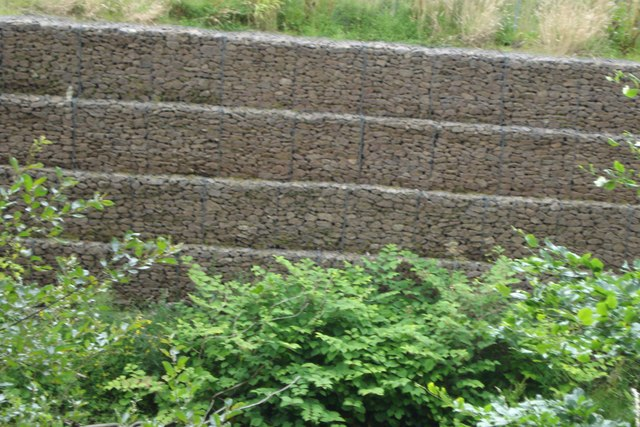
\includegraphics[keepaspectratio]{capitulos/../img/gabiao_rio.jpg}}

}

\caption{\label{fig-gabiao-rio}Gabião convencional em margem fluvial ---
estrutura metálica preenchida com pedras.}

\end{figure}%

\end{minipage}%
%
\begin{minipage}{0.50\linewidth}

\begin{figure}[H]

\centering{

\pandocbounded{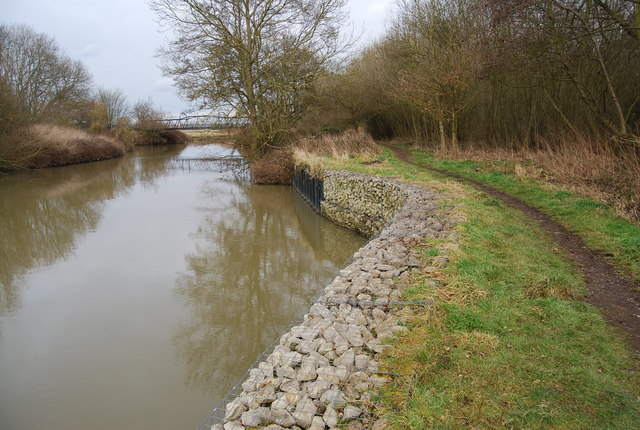
\includegraphics[keepaspectratio]{capitulos/../img/gabiao_medway.jpg}}

}

\caption{\label{fig-gabiao-vivo}Gabião vivo com vegetação emergente ---
a transição funcional da resistência mecânica para a ancoragem
biológica.}

\end{figure}%

\end{minipage}%

\end{figure}%

\section{Transição Estrutural}\label{transiuxe7uxe3o-estrutural}

O ciclo de vida do gabião vivo segue três fases distintas, conforme
sintetizado na Tabela~\ref{tbl-transicao}. Na fase estrutural (0--5
anos), a estabilidade é garantida integralmente pelo arame e pelas
pedras, enquanto as estacas vivas desenvolvem seu sistema radicular. Na
fase de transição (5--15 anos), as raízes já contribuem
significativamente para a coesão do conjunto, compartilhando a função de
resistência com o arame que ainda mantém integridade parcial. Na fase
biológica (15--25+ anos), o arame corroído perde função estrutural, mas
o sistema radicular já desenvolveu coesão suficiente (15--25 kPa de
coesão radicular) para manter a estabilidade do conjunto, que funciona
então como um maciço de solo reforçado por raízes com pedras que
contribuem com peso e drenagem.

\begin{longtable}[]{@{}
  >{\raggedright\arraybackslash}p{(\linewidth - 8\tabcolsep) * \real{0.0741}}
  >{\raggedright\arraybackslash}p{(\linewidth - 8\tabcolsep) * \real{0.1111}}
  >{\raggedright\arraybackslash}p{(\linewidth - 8\tabcolsep) * \real{0.2716}}
  >{\raggedright\arraybackslash}p{(\linewidth - 8\tabcolsep) * \real{0.2716}}
  >{\raggedright\arraybackslash}p{(\linewidth - 8\tabcolsep) * \real{0.2716}}@{}}
\caption{Fases da transição funcional do gabião
vivo.}\label{tbl-transicao}\tabularnewline
\toprule\noalign{}
\begin{minipage}[b]{\linewidth}\raggedright
Fase
\end{minipage} & \begin{minipage}[b]{\linewidth}\raggedright
Período
\end{minipage} & \begin{minipage}[b]{\linewidth}\raggedright
Resistência dominante
\end{minipage} & \begin{minipage}[b]{\linewidth}\raggedright
Contribuição do arame
\end{minipage} & \begin{minipage}[b]{\linewidth}\raggedright
Contribuição radicular
\end{minipage} \\
\midrule\noalign{}
\endfirsthead
\toprule\noalign{}
\begin{minipage}[b]{\linewidth}\raggedright
Fase
\end{minipage} & \begin{minipage}[b]{\linewidth}\raggedright
Período
\end{minipage} & \begin{minipage}[b]{\linewidth}\raggedright
Resistência dominante
\end{minipage} & \begin{minipage}[b]{\linewidth}\raggedright
Contribuição do arame
\end{minipage} & \begin{minipage}[b]{\linewidth}\raggedright
Contribuição radicular
\end{minipage} \\
\midrule\noalign{}
\endhead
\bottomrule\noalign{}
\endlastfoot
Estrutural & 0--5 anos & Arame + pedras & 100\% & 0--20\% \\
Transição & 5--15 anos & Arame + raízes & 60--40\% & 40--60\% \\
Biológica & 15--25+ anos & Raízes + pedras & 0--20\% & 80--100\% \\
\end{longtable}

\begin{tcolorbox}[enhanced jigsaw, leftrule=.75mm, colframe=quarto-callout-note-color-frame, colback=white, bottomrule=.15mm, opacityback=0, colbacktitle=quarto-callout-note-color!10!white, breakable, bottomtitle=1mm, opacitybacktitle=0.6, title=\textcolor{quarto-callout-note-color}{\faInfo}\hspace{0.5em}{Conceito-chave}, titlerule=0mm, toprule=.15mm, toptitle=1mm, rightrule=.15mm, left=2mm, arc=.35mm, coltitle=black]

A cesta de arame galvanizado tem vida útil de 15--25 anos. Quando o
arame se deteriora, o sistema radicular já deve ter desenvolvido coesão
suficiente (15--25 kPa) para manter a estabilidade. Essa é a premissa
central do projeto: o dimensionamento deve garantir que a taxa de
crescimento radicular supere a taxa de corrosão do arame, criando uma
janela de segurança na transição.

\end{tcolorbox}

\section{Dimensionamento Estrutural}\label{dimensionamento-estrutural}

O dimensionamento segue os mesmos princípios das estruturas de contenção
por gravidade, exigindo três verificações de estabilidade obrigatórias.

\subsection{Verificação ao
Tombamento}\label{verificauxe7uxe3o-ao-tombamento}

A estrutura deve ser verificada contra rotação em torno da aresta
inferior da base, garantindo que os momentos resistentes (peso próprio e
eventuais sobrecargas favoráveis) superem os momentos atuantes (empuxo
de terra) com fator de segurança mínimo de 1,5

\[
FS_{tomb} = \frac{M_{resistente}}{M_{atuante}} \geq 1{,}5
\]

\subsection{Verificação ao
Deslizamento}\label{verificauxe7uxe3o-ao-deslizamento}

A resistência ao deslizamento na base da estrutura deve superar o empuxo
ativo horizontal do solo com fator de segurança mínimo de 1,5

\[
FS_{desl} = \frac{N \cdot \tan \phi + c \cdot B}{E_a} \geq 1{,}5
\]

onde \(N\) é a força normal na base (peso próprio da estrutura),
\(\phi\) é o ângulo de atrito na interface solo-gabião (tipicamente
30--35° para pedregulho sobre solo compactado), \(c\) é a coesão na base
(se houver), \(B\) é a largura da base do gabião e \(E_a\) é o empuxo
ativo calculado pela teoria de Rankine ou Coulomb.

\subsection{Verificação da Capacidade de
Carga}\label{verificauxe7uxe3o-da-capacidade-de-carga}

A tensão máxima transmitida ao solo de fundação não deve exceder a
capacidade de carga admissível do solo

\[
FS_{cap} = \frac{q_{ult}}{q_{atuante}} \geq 3{,}0
\]

onde \(q_{ult}\) é a capacidade de carga última do solo de fundação,
determinada por ensaios de campo (SPT, CPT) ou por formulações teóricas
(Terzaghi, Meyerhof).

\section{Construção}\label{construuxe7uxe3o-1}

\subsection{Materiais}\label{materiais-2}

A construção do gabião vivo exige cestas de tela de arame galvanizado de
dupla torção (malha 8×10 cm, Ø 2,7--3,4 mm), conforme ABNT NBR 10514,
que devem ser inspecionadas quanto à integridade da galvanização antes
da montagem. As pedras devem ter diâmetro de 10--25 cm, ser compactas,
resistentes ao intemperismo e não friáveis (teste de fragmentação
manual). As estacas vivas (ramos de 2--5 cm de diâmetro, com comprimento
igual à largura do gabião mais 30 cm para cada lado) devem ser de
espécies com alta taxa de brotação vegetativa. O solo vegetal para
preenchimento dos interstícios deve ser uma mistura de solo local com
15--20\% de composto orgânico, garantindo fertilidade e retenção hídrica
para o desenvolvimento radicular.

\subsection{Passo a Passo}\label{passo-a-passo-1}

A construção inicia com a preparação da fundação, que consiste na
escavação de uma trincheira de encastramento de 30--50 cm de
profundidade e largura igual à base do gabião, regularizada e
compactada. As cestas metálicas são então montadas e amarradas com arame
da mesma especificação, posicionadas na trincheira e iniciado o
preenchimento. O preenchimento é realizado em camadas de 1/3 da altura
total, intercalando-se pedras arranjadas manualmente (não despejadas
aleatoriamente, para evitar vazios excessivos), estacas vivas
horizontais (com pontas projetando 20--30 cm da face frontal para
permitir brotação e exposição à luz) e solo vegetal nos interstícios
entre as pedras. Após a primeira e a segunda camada, instalam-se
tirantes internos de arame, tensionados entre as faces frontal e
posterior, para manter a geometria da cesta sob carga e prevenir o
abaulamento. Após a terceira camada e os tirantes superiores, fecha-se e
amarra-se a tampa. O procedimento finaliza com o plantio de gramíneas e
herbáceas na face frontal exposta, utilizando sementes ou mudas
inseridas nos interstícios superficiais.

\section{Coesão Radicular}\label{coesuxe3o-radicular}

O incremento de coesão proporcionado pelo sistema radicular é o
mecanismo central que garante a funcionalidade de longo prazo do gabião
vivo. O crescimento segue uma curva sigmoidal, com fase inicial lenta
(enraizamento e adaptação), fase exponencial (rápido desenvolvimento
radicular) e fase de estabilização (maturidade do sistema)

\[
c_r(t) = c_{r,max} \cdot \frac{1}{1 + e^{-k(t - t_0)}}
\]

onde \(c_{r,max}\) é a coesão radicular máxima (15--25 kPa para espécies
arbóreas tropicais), \(k\) é a taxa de crescimento (parâmetro
espécie-específico) e \(t_0\) é o tempo de inflexão da curva
(tipicamente 5--8 anos para espécies tropicais de rápido crescimento). A
importância prática dessa equação é que ela permite ao projetista
estimar em que ano a contribuição radicular atingirá o limiar necessário
para compensar a perda de integridade do arame, validando a viabilidade
da transição funcional.

\section{Normas Aplicáveis}\label{normas-aplicuxe1veis}

O projeto e a construção de gabiões vivos devem atender a um conjunto de
normas técnicas que regem tanto a componente estrutural metálica quanto
os critérios de estabilidade geotécnica. No âmbito brasileiro,
aplicam-se a ABNT NBR 10514 (gabiões e colchões reno, que especifica
materiais, fabricação e montagem), a DNIT 062 (especificação para
contenções com gabiões em obras rodoviárias). No âmbito internacional,
aplicam-se a ASTM A975 (gabião metálico, incluindo requisitos de
galvanização e resistência mecânica da malha) e a EN 10223-3 (tela de
dupla torção, requisitos dimensionais e mecânicos da malha hexagonal).

\section{Custos Comparativos}\label{custos-comparativos-1}

A Tabela~\ref{tbl-custos-gabiao} compara o custo por metro cúbico de
diferentes soluções de contenção, posicionando o gabião vivo no contexto
das alternativas disponíveis.

\begin{longtable}[]{@{}lll@{}}
\caption{Custos comparativos de estruturas de
contenção.}\label{tbl-custos-gabiao}\tabularnewline
\toprule\noalign{}
Solução & Custo (R\$/m³) & Vida útil estimada \\
\midrule\noalign{}
\endfirsthead
\toprule\noalign{}
Solução & Custo (R\$/m³) & Vida útil estimada \\
\midrule\noalign{}
\endhead
\bottomrule\noalign{}
\endlastfoot
Gabião convencional & 350--550 & 15--25 anos (limitada pelo arame) \\
Gabião vivo & 400--650 & 50+ anos (transição biológica) \\
Muro de concreto armado & 800--1.500 & 50--80 anos \\
Solo reforçado com geossintético & 500--900 & 30--50 anos \\
\end{longtable}

O gabião vivo apresenta sobrecusto de 15--20\% em relação ao gabião
convencional, equivalente ao custo das estacas vivas, do solo vegetal e
da mão de obra adicional de plantio. Esse investimento adicional é
recuperado pela extensão da vida útil funcional (de 15--25 para 50+
anos), pela eliminação da necessidade de substituição periódica das
cestas corroídas e pelos serviços ecossistêmicos gerados (habitat,
paisagem, carbono), que conferem ao gabião vivo uma relação
custo-benefício de ciclo de vida (LCC) superior a todas as alternativas
listadas.

\chapter{Parede Krainer}\label{parede-krainer}

\# Parede Krainer \{\#sec-parede-krainer\}

A parede Krainer (\emph{Krainer wall} ou \emph{crib wall}) é uma
estrutura de contenção em grelha de troncos de madeira preenchida com
solo e vegetação. Originária dos Alpes austríacos (região da Caríntia),
foi desenvolvida para estabilizar encostas montanhosas e margens de rios
torrenciais, sendo posteriormente adaptada para uso em regiões tropicais
utilizando madeiras locais (eucalipto, sabiá, acácia). O princípio
construtivo é elegante em sua simplicidade: troncos dispostos em grelha
tridimensional formam células prismáticas que são preenchidas com solo,
funcionando como uma estrutura de contenção por gravidade (resistência
pelo peso próprio) com capacidade de autovegetação nas faces e no topo.

A principal vantagem da parede Krainer sobre muros de concreto armado ou
gabiões é a integração paisagística: após 2--3 anos, a vegetação cobre
completamente a estrutura, que se torna indistinguível de um talude
natural vegetado. Essa característica é particularmente valorizada em
áreas de proteção ambiental, margens de rios em zonas urbanas e taludes
viários em regiões turísticas. A Figura~\ref{fig-krainer} mostra uma
parede Krainer instalada, onde se observa a grelha de troncos e o
preenchimento com solo, com vegetação em processo de colonização da face
frontal.

\begin{figure}

\centering{

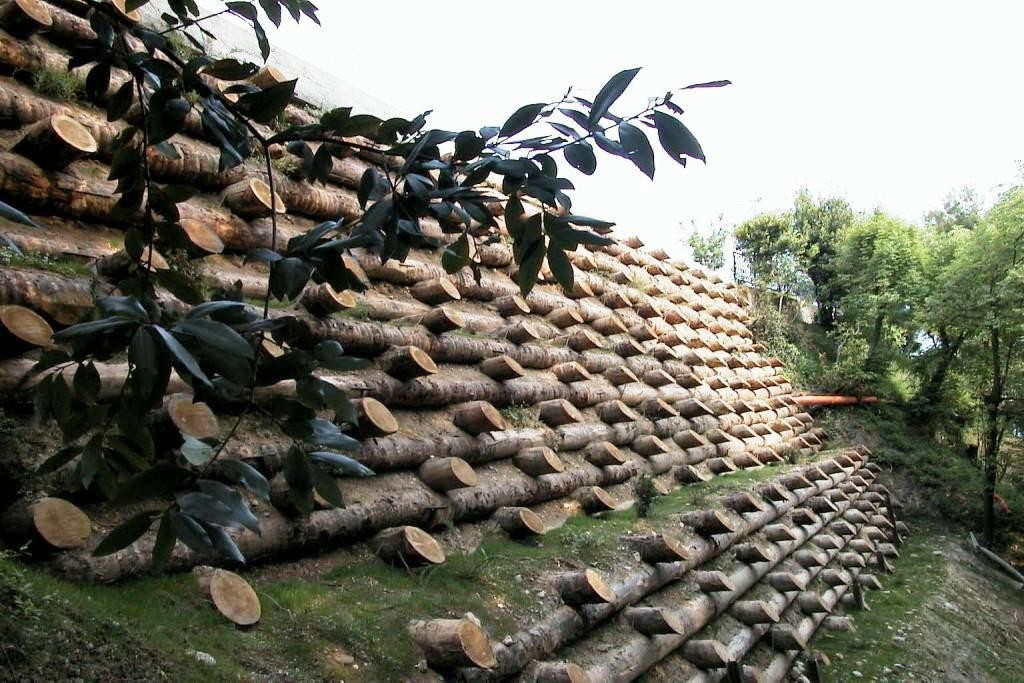
\includegraphics[width=0.8\linewidth,height=\textheight,keepaspectratio]{capitulos/../img/krainer_1.jpg}

}

\caption{\label{fig-krainer}Parede Krainer instalada --- grelha de
troncos preenchida com solo e vegetação para contenção de encostas.}

\end{figure}%

\section{Tipologia}\label{tipologia}

A parede Krainer pode ser construída em duas configurações estruturais,
cuja escolha depende da altura necessária e das solicitações mecânicas.
A Figura~\ref{fig-krainer2} mostra uma parede Krainer dupla em estágio
avançado de colonização vegetal, enquanto a
Figura~\ref{fig-krainer-corte} apresenta o corte transversal esquemático
que detalha o arranjo construtivo dos troncos e o preenchimento com
solo.

\begin{figure}

\begin{minipage}{0.50\linewidth}

\begin{figure}[H]

\centering{

\pandocbounded{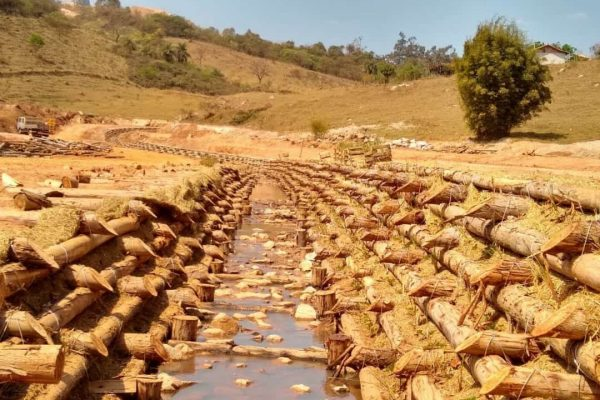
\includegraphics[keepaspectratio]{capitulos/../img/krainer_2.jpg}}

}

\caption{\label{fig-krainer2}Parede Krainer dupla em estágio avançado
--- vegetação já estabelecida entre os troncos.}

\end{figure}%

\end{minipage}%
%
\begin{minipage}{0.50\linewidth}

\begin{figure}[H]

\centering{

\pandocbounded{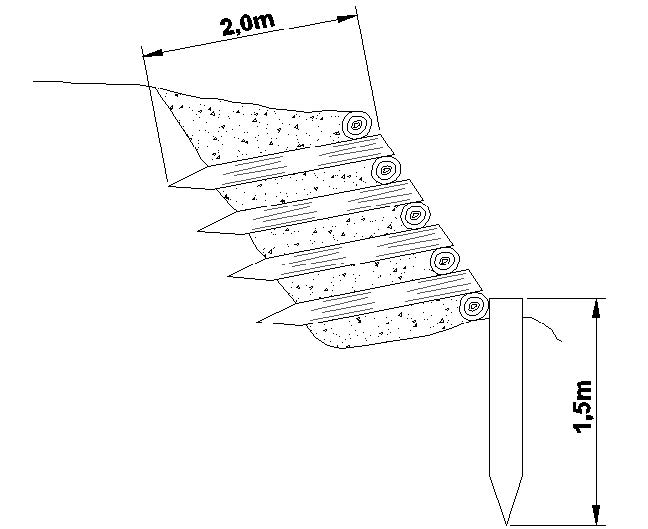
\includegraphics[keepaspectratio]{capitulos/../img/krainer_corte.jpeg}}

}

\caption{\label{fig-krainer-corte}Corte transversal esquemático da
parede Krainer --- mostrando o arranjo de troncos e o preenchimento com
solo.}

\end{figure}%

\end{minipage}%

\end{figure}%

\subsection{Parede Krainer Simples}\label{parede-krainer-simples}

A parede simples consiste em uma grelha de troncos em uma única direção
(longitudinal), apoiados em troncos transversais curtos que funcionam
como consolos. A altura máxima recomendada é de 2,0 m, adequada para
estabilização de pequenos taludes, bases de encostas e cabeceiras de
voçorocas. A profundidade de embutimento (comprimento dos troncos
transversais) deve ser de pelo menos 0,5× a altura, garantindo ancoragem
suficiente no maciço de solo a montante.

\subsection{Parede Krainer Dupla}\label{parede-krainer-dupla}

A parede dupla emprega grelha de troncos em duas direções (longitudinal
+ transversal), formando células prismáticas tridimensionais de alta
estabilidade mecânica. A altura máxima recomendada é de 4,0 m, sendo a
configuração adequada para margens fluviais, taludes viários de grande
altura e encostas com risco geotécnico. A robustez estrutural é
significativamente superior à da parede simples, pois os troncos
transversais atravessam toda a seção da parede (não são consolos) e
criam intertravamento mecânico em ambas as direções.

\section{Dimensionamento Estrutural}\label{dimensionamento-estrutural-1}

O dimensionamento da parede Krainer segue os princípios das estruturas
de contenção por gravidade, de forma análoga ao gabião vivo (ver
\textbf{?@sec-gabiao-vivo}).

\subsection{Geometria}\label{geometria}

A base (\(B\)) da parede deve ser igual ou superior a \(0{,}5 \cdot H\)
(mínimo absoluto de 1,0 m), onde \(H\) é a altura total da parede. A
altura máxima (\(H\)) é de 4,0 m para paredes duplas e 2,0 m para
simples. A face frontal deve ter inclinação de 10 a 15° em relação à
vertical (inclinada para trás), o que desloca o centro de gravidade para
o interior do maciço e melhora a segurança ao tombamento. Os troncos
devem ter diâmetro de 15--30 cm (diâmetros maiores para paredes mais
altas), com espaçamento entre troncos longitudinais de 30--60 cm (vãos
que permitem a passagem de vegetação e drenagem sem comprometer a
retenção do solo de preenchimento).

\subsection{Verificação de
Estabilidade}\label{verificauxe7uxe3o-de-estabilidade}

As verificações de estabilidade seguem as mesmas expressões apresentadas
para o gabião vivo

\[
FS_{tomb} \geq 1{,}5 \quad;\quad FS_{desl} \geq 1{,}5 \quad;\quad FS_{cap} \geq 3{,}0
\]

\subsection{Peso Específico da
Estrutura}\label{peso-especuxedfico-da-estrutura}

Para o cálculo das forças resistentes, é necessário determinar o peso
específico aparente da estrutura preenchida (\(\gamma_{ap}\)), que
depende da proporção volumétrica de madeira e solo no interior da grelha

\[
\gamma_{ap} = n_{madeira} \cdot \gamma_{madeira} + (1 - n_{madeira}) \cdot \gamma_{solo}
\]

onde \(n_{madeira}\) é a fração volumétrica da madeira (tipicamente
15--25\%, dependendo do diâmetro dos troncos e do espaçamento),
\(\gamma_{madeira}\) é o peso específico da madeira (5--10 kN/m³,
conforme a espécie) e \(\gamma_{solo}\) é o peso específico do solo de
preenchimento compactado (16--20 kN/m³). Para uma parede com 20\% de
madeira de eucalipto (\(\gamma = 7\) kN/m³) e solo compactado
(\(\gamma = 18\) kN/m³), \(\gamma_{ap} \approx 15{,}8\) kN/m³.

\section{Seleção de Madeiras
Tropicais}\label{seleuxe7uxe3o-de-madeiras-tropicais}

A durabilidade da madeira é o fator limitante da vida útil da componente
estrutural da parede Krainer. A seleção deve considerar a durabilidade
natural (resistência à biodeterioração sem tratamento), a densidade (que
influencia o peso específico e a resistência mecânica) e a
disponibilidade regional. A Tabela~\ref{tbl-madeiras} compara as
principais opções para o contexto tropical brasileiro.

\begin{longtable}[]{@{}
  >{\raggedright\arraybackslash}p{(\linewidth - 6\tabcolsep) * \real{0.1364}}
  >{\raggedright\arraybackslash}p{(\linewidth - 6\tabcolsep) * \real{0.2879}}
  >{\raggedright\arraybackslash}p{(\linewidth - 6\tabcolsep) * \real{0.3182}}
  >{\raggedright\arraybackslash}p{(\linewidth - 6\tabcolsep) * \real{0.2576}}@{}}
\caption{Madeiras tropicais para paredes
Krainer.}\label{tbl-madeiras}\tabularnewline
\toprule\noalign{}
\begin{minipage}[b]{\linewidth}\raggedright
Espécie
\end{minipage} & \begin{minipage}[b]{\linewidth}\raggedright
Densidade (kg/m³)
\end{minipage} & \begin{minipage}[b]{\linewidth}\raggedright
Durabilidade natural
\end{minipage} & \begin{minipage}[b]{\linewidth}\raggedright
Disponibilidade
\end{minipage} \\
\midrule\noalign{}
\endfirsthead
\toprule\noalign{}
\begin{minipage}[b]{\linewidth}\raggedright
Espécie
\end{minipage} & \begin{minipage}[b]{\linewidth}\raggedright
Densidade (kg/m³)
\end{minipage} & \begin{minipage}[b]{\linewidth}\raggedright
Durabilidade natural
\end{minipage} & \begin{minipage}[b]{\linewidth}\raggedright
Disponibilidade
\end{minipage} \\
\midrule\noalign{}
\endhead
\bottomrule\noalign{}
\endlastfoot
\emph{Eucalyptus} spp. & 550--800 & 5--15 anos & Alta \\
\emph{Mimosa caesalpiniifolia} (sabiá) & 800--1.000 & 10--20 anos &
Média (Nordeste) \\
\emph{Acacia mangium} & 500--650 & 5--10 anos & Média \\
\emph{Bambusa} spp. (bambu) & 400--700 & 3--5 anos (tratado) & Alta \\
\emph{Tectona grandis} (teca) & 550--700 & 20+ anos & Baixa \\
\end{longtable}

No contexto tropical brasileiro, o eucalipto tratado é a escolha mais
frequente pela combinação de alta disponibilidade e custo acessível,
embora sua durabilidade natural seja inferior à do sabiá (\emph{Mimosa
caesalpiniifolia}), espécie nativa do Nordeste cuja madeira extremamente
densa (800--1.000 kg/m³) dispensa tratamento químico em muitas
aplicações. O bambu, apesar de abundante, é recomendado somente para
estruturas temporárias (3--5 anos mesmo com tratamento), enquanto a teca
oferece a melhor durabilidade natural (20+ anos), porém com
disponibilidade e custo limitantes para projetos de grande escala.

\begin{tcolorbox}[enhanced jigsaw, leftrule=.75mm, colframe=quarto-callout-tip-color-frame, colback=white, bottomrule=.15mm, opacityback=0, colbacktitle=quarto-callout-tip-color!10!white, breakable, bottomtitle=1mm, opacitybacktitle=0.6, title=\textcolor{quarto-callout-tip-color}{\faLightbulb}\hspace{0.5em}{Tratamento preservativo}, titlerule=0mm, toprule=.15mm, toptitle=1mm, rightrule=.15mm, left=2mm, arc=.35mm, coltitle=black]

Madeiras não naturalmente duráveis devem receber tratamento com CCA
(Arseniato de Cobre Cromatado) ou CCB (Borato de Cobre Cromatado) em
autoclave, que impregna a madeira com sais metálicos fungicidas e
inseticidas sob pressão, aumentando a durabilidade para 15--25 anos. O
tratamento deve ser realizado com a madeira já cortada nas dimensões de
projeto, pois cortes posteriores expõem o cerne não tratado à
biodeterioração.

\end{tcolorbox}

\section{Estacas Vivas}\label{estacas-vivas-1}

A inserção de estacas vivas entre os troncos é o elemento que diferencia
a parede Krainer convencional (estrutura exclusivamente de madeira
morta) da versão de bioengenharia de solos. As estacas são segmentos de
ramos de espécies com alta capacidade de propagação vegetativa, as
mesmas empregadas em gabiões vivos e enrocamento vegetado (ver
\textbf{?@sec-gabiao-vivo} e \textbf{?@sec-enrocamento}), com diâmetro
de 3--8 cm e comprimento suficiente para transpor toda a seção da parede
mais 30 cm para cada lado (garantindo contato com o solo natural a
montante e exposição à luz na face frontal). As estacas são inseridas
horizontalmente entre camadas de troncos, em densidade de 3--5 estacas
por m² de face, preferencialmente durante o período de dormência
vegetativa (estação seca) para maximizar as taxas de enraizamento. Com o
brotamento e o desenvolvimento radicular, as estacas desempenham três
funções simultâneas: reforço mecânico do solo de preenchimento por
coesão radicular, drenagem biológica por evapotranspiração e integração
paisagística progressiva.

\section{Construção}\label{construuxe7uxe3o-2}

O arranjo tridimensional da estrutura pode ser visualizado na
Figura~\ref{fig-krainer-3d}, enquanto a Figura~\ref{fig-krainer-pecas}
detalha as peças componentes individuais (troncos longitudinais,
transversais e estacas vivas) e sua posição relativa no conjunto.

\begin{figure}

\begin{minipage}{0.50\linewidth}

\begin{figure}[H]

\centering{

\pandocbounded{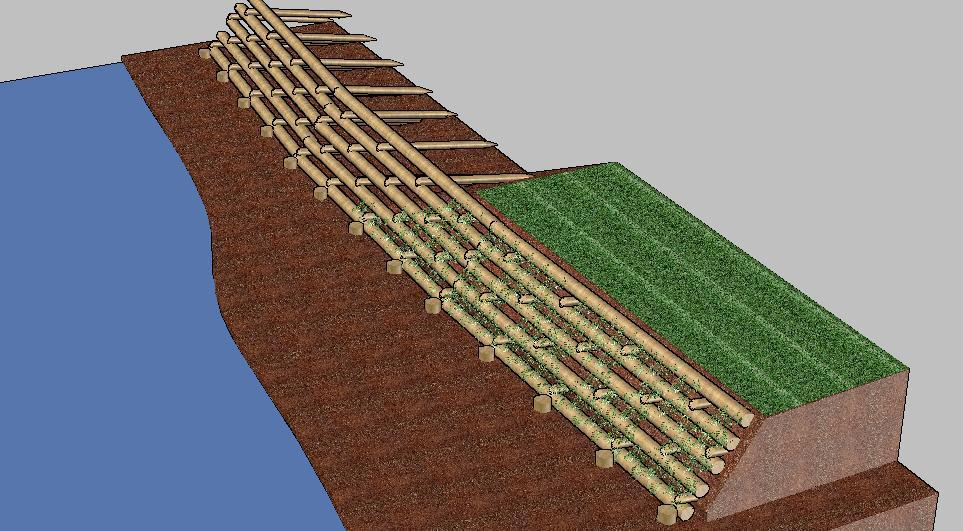
\includegraphics[keepaspectratio]{capitulos/../img/krainer_3d.jpeg}}

}

\caption{\label{fig-krainer-3d}Vista tridimensional da parede Krainer
--- arranjo estrutural dos troncos longitudinais e transversais formando
células prismáticas.}

\end{figure}%

\end{minipage}%
%
\begin{minipage}{0.50\linewidth}

\begin{figure}[H]

\centering{

\pandocbounded{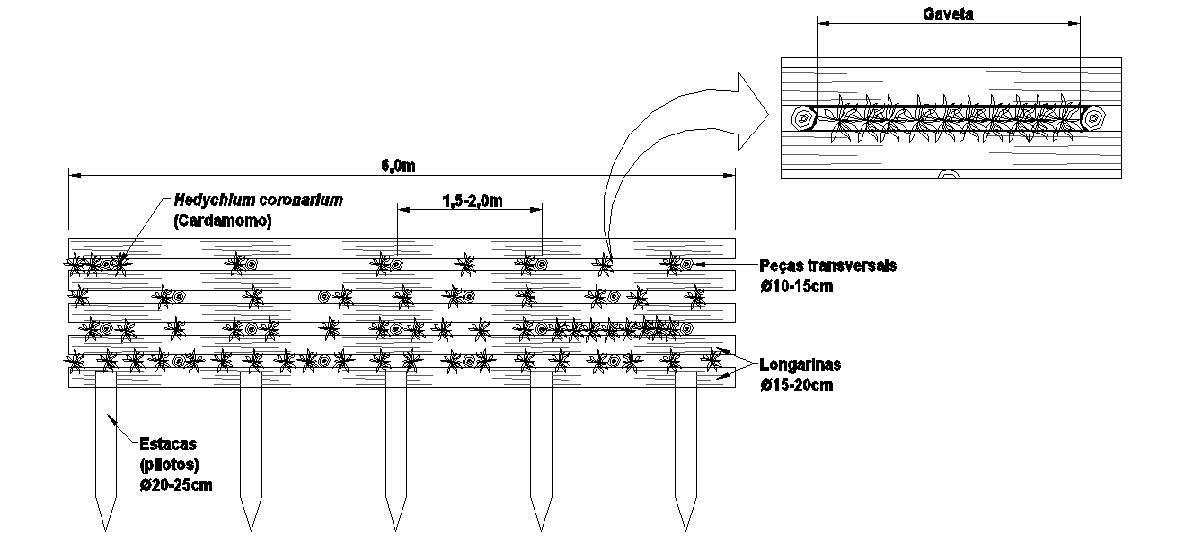
\includegraphics[keepaspectratio]{capitulos/../img/krainer_pecas.jpeg}}

}

\caption{\label{fig-krainer-pecas}Peças componentes da parede Krainer
--- troncos longitudinais, transversais e estacas vivas antes da
montagem.}

\end{figure}%

\end{minipage}%

\end{figure}%

A construção segue uma sequência de empilhamento por camadas. A primeira
etapa consiste na escavação da fundação, uma trincheira de encastramento
com profundidade de 40--60 cm e largura igual à base de projeto (\(B\)),
nivelada e compactada para distribuir as tensões de contato. Na segunda
etapa, os troncos longitudinais de base são posicionados na trincheira
com o espaçamento definido (30--60 cm), e os troncos transversais são
apoiados perpendicularmente sobre eles, fixados com pregos de aço
galvanizado (\(\varnothing\) 8--10 mm) ou parafusos estruturais nos
pontos de cruzamento. Na terceira etapa, as células formadas pela grelha
são preenchidas com solo vegetal em camadas de 15--20 cm, levemente
compactadas (compactação excessiva impede o desenvolvimento radicular
das estacas vivas). A quarta etapa consiste na inserção horizontal das
estacas vivas entre os troncos, com a extremidade basal voltada para o
interior do maciço (contato com umidade) e a extremidade apical
ligeiramente projetada na face frontal. Esse ciclo de empilhamento
(troncos → fixação → preenchimento → estacas vivas) é repetido até
atingir a altura de projeto, finalizando com o plantio de gramíneas e
arbustos no topo e nas faces expostas para proteção superficial imediata
contra erosão laminar.

\section{Drenagem}\label{drenagem}

A parede Krainer é intrinsecamente autordrenante graças aos espaços
entre troncos, que funcionam como canais de percolação distribuídos ao
longo de toda a face frontal, impedindo o acúmulo de poropressões
positivas no interior da estrutura (fator crítico de instabilidade em
muros de arrimo convencionais). No entanto, em solos com alto teor de
finos (siltes e argilas dispersivas), os espaços entre troncos podem ser
gradualmente colmatados pelo carreamento de partículas finas, reduzindo
a capacidade drenante. Para esses casos, recomenda-se a instalação de
barbacãs de PVC (\(\varnothing\) 50 mm) a cada 2--3 m² de face, com
inclinação descendente de 5° para o exterior, além de uma camada de
brita ou manta geotêxtil não tecida na interface entre o solo de
preenchimento e a face frontal da parede, funcionando como filtro que
retém finos mas permite a passagem de água.

\section{Aplicações}\label{aplicauxe7uxf5es-1}

A Tabela~\ref{tbl-aplicacoes} sintetiza as aplicações típicas da parede
Krainer, indicando a altura usual e o tipo de parede recomendado para
cada cenário. A versatilidade da técnica permite seu emprego desde
pequenas intervenções em cabeceiras de voçorocas até obras de maior
porte em margens fluviais, sempre com a vantagem da progressiva
integração paisagística que elimina a necessidade de revestimentos
estéticos posteriores.

\begin{longtable}[]{@{}
  >{\raggedright\arraybackslash}p{(\linewidth - 6\tabcolsep) * \real{0.2075}}
  >{\raggedright\arraybackslash}p{(\linewidth - 6\tabcolsep) * \real{0.2642}}
  >{\raggedright\arraybackslash}p{(\linewidth - 6\tabcolsep) * \real{0.3019}}
  >{\raggedright\arraybackslash}p{(\linewidth - 6\tabcolsep) * \real{0.2264}}@{}}
\caption{Aplicações típicas da parede
Krainer.}\label{tbl-aplicacoes}\tabularnewline
\toprule\noalign{}
\begin{minipage}[b]{\linewidth}\raggedright
Aplicação
\end{minipage} & \begin{minipage}[b]{\linewidth}\raggedright
Altura típica
\end{minipage} & \begin{minipage}[b]{\linewidth}\raggedright
Tipo de parede
\end{minipage} & \begin{minipage}[b]{\linewidth}\raggedright
Observação
\end{minipage} \\
\midrule\noalign{}
\endfirsthead
\toprule\noalign{}
\begin{minipage}[b]{\linewidth}\raggedright
Aplicação
\end{minipage} & \begin{minipage}[b]{\linewidth}\raggedright
Altura típica
\end{minipage} & \begin{minipage}[b]{\linewidth}\raggedright
Tipo de parede
\end{minipage} & \begin{minipage}[b]{\linewidth}\raggedright
Observação
\end{minipage} \\
\midrule\noalign{}
\endhead
\bottomrule\noalign{}
\endlastfoot
Margens de rios & 1,5--3,0 m & Dupla & Exige proteção de base contra
solapamento \\
Taludes viários & 1,0--2,5 m & Simples ou dupla & Compatível com
paisagismo rodoviário \\
Estabilização de encostas & 2,0--4,0 m & Dupla & Pode ser escalonada em
bancadas \\
Controle de voçorocas & 1,0--2,0 m & Simples & Associar a paliçadas a
montante (\textbf{?@sec-palicadas}) \\
\end{longtable}

\chapter{Canaleta Verde}\label{canaleta-verde}

\# Canaleta Verde \{\#sec-canaleta-verde\}

A canaleta verde (\emph{vegetated swale} ou \emph{bioswale}) é um canal
de drenagem aberto com seção trapezoidal ou parabólica, revestido com
vegetação herbácea densa, que funciona simultaneamente como condutor
hidráulico e como sistema de tratamento por infiltração e filtração.
Diferentemente das canaletas de concreto (estruturas impermeáveis que
apenas transportam o escoamento), a canaleta verde intercepta,
desacelera e filtra o escoamento superficial, promovendo a remoção de
sedimentos, nutrientes e poluentes difusos antes que atinjam os corpos
hídricos receptores. A Figura~\ref{fig-canaleta} ilustra uma canaleta
verde com vegetação herbácea plenamente estabelecida, onde a rugosidade
da cobertura vegetal reduz a velocidade do escoamento e a superfície
permeável permite infiltração ao longo de todo o percurso.

\begin{figure}

\centering{

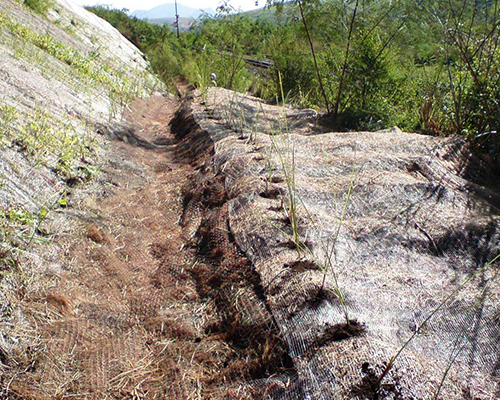
\includegraphics[width=0.8\linewidth,height=\textheight,keepaspectratio]{capitulos/../img/canaleta_verde.jpg}

}

\caption{\label{fig-canaleta}Canaleta verde com vegetação herbácea
estabelecida --- canal de drenagem naturalizado que combina condução
hidráulica com tratamento por infiltração.}

\end{figure}%

\section{Funções}\label{funuxe7uxf5es-1}

A canaleta verde desempenha cinco funções hidráulicas e ambientais
simultâneas, o que justifica sua classificação como técnica de
infraestrutura verde multifuncional. A primeira é a condução controlada
do escoamento superficial, substituindo tubulações enterradas por um
canal aberto que pode ser inspecionado visualmente e mantido com baixo
custo operacional. A segunda é a infiltração para recarga do aquífero,
com taxas que dependem da permeabilidade do solo subjacente e da altura
da vegetação (canaletas em solos arenosos podem infiltrar 30--60\% do
volume escoado). A terceira é a filtração de sedimentos e nutrientes
pela interação entre o escoamento e a vegetação densa, que funciona como
filtro biológico com eficiência de remoção de 60--85\% para sólidos
suspensos. A quarta é o amortecimento do pico de cheia por laminação, em
que a rugosidade vegetal retarda o escoamento e distribui o hidrograma
ao longo de um período mais prolongado. A quinta é a integração
paisagística com geração de serviços ecossistêmicos (habitat para
polinizadores, corredor ecológico, sequestro de carbono). A
Figura~\ref{fig-canaleta-hidro} mostra a integração entre a canaleta
verde e a técnica de hidrossemeadura (ver
\textbf{?@sec-hidrossemeadura}), utilizada para o estabelecimento rápido
da cobertura vegetal protetora no canal recém-construído.

\begin{figure}

\centering{

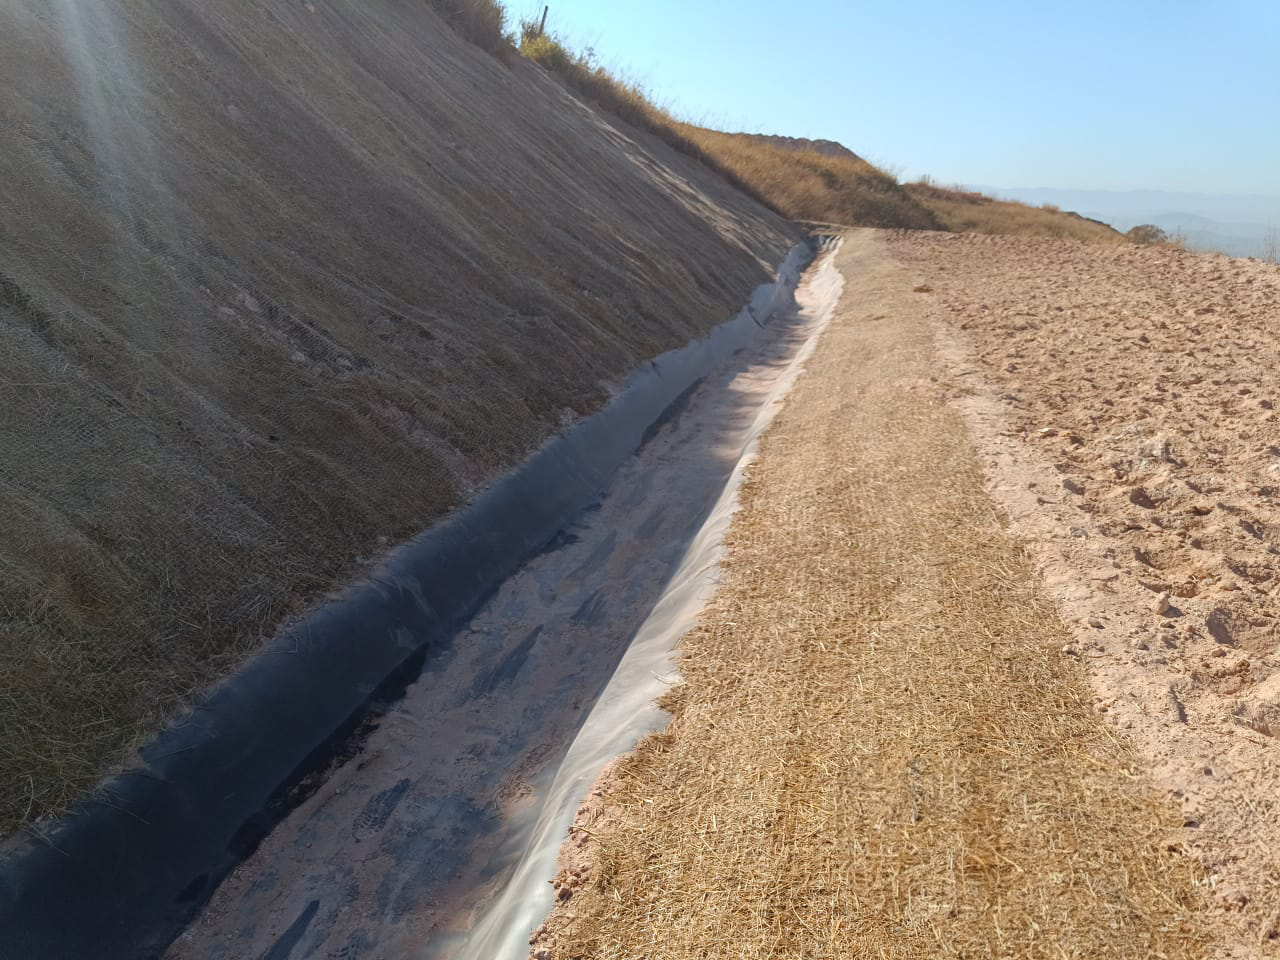
\includegraphics[width=0.8\linewidth,height=\textheight,keepaspectratio]{capitulos/../img/canaleta_hidrossemeadura.png}

}

\caption{\label{fig-canaleta-hidro}Canaleta verde com hidrossemeadura
--- integração de drenagem naturalizada com revegetação por
hidrossemeadura para estabelecimento rápido da cobertura vegetal.}

\end{figure}%

\section{Dimensionamento
Hidráulico}\label{dimensionamento-hidruxe1ulico}

O dimensionamento hidráulico da canaleta verde segue os mesmos
princípios aplicados a canais abertos em regime permanente e uniforme,
com a particularidade de que o coeficiente de resistência ao escoamento
(\(n\) de Manning) é significativamente maior do que em canais
revestidos com concreto, pois a rugosidade da vegetação é o elemento que
confere à canaleta suas funções de filtração e amortecimento.

\subsection{Equação de Manning}\label{equauxe7uxe3o-de-manning}

A vazão de projeto (\(Q\)) é calculada pela equação de Manning para
escoamento uniforme em canais abertos

\[
Q = \frac{1}{n} \cdot A \cdot R_h^{2/3} \cdot S^{1/2}
\]

onde \(Q\) é a vazão (m³/s), \(n\) é o coeficiente de Manning
(adimensional, função da rugosidade vegetal), \(A\) é a área da seção
molhada (m²), \(R_h\) é o raio hidráulico (\(A/P\), onde \(P\) é o
perímetro molhado, em metros), e \(S\) é a declividade longitudinal do
canal (m/m). Para canais vegetados, o coeficiente \(n\) varia com a
espécie, a altura e a densidade da vegetação, conforme a
Tabela~\ref{tbl-manning}.

\begin{longtable}[]{@{}
  >{\raggedright\arraybackslash}p{(\linewidth - 4\tabcolsep) * \real{0.4130}}
  >{\raggedright\arraybackslash}p{(\linewidth - 4\tabcolsep) * \real{0.3261}}
  >{\raggedright\arraybackslash}p{(\linewidth - 4\tabcolsep) * \real{0.2609}}@{}}
\caption{Coeficientes de Manning para canais
vegetados.}\label{tbl-manning}\tabularnewline
\toprule\noalign{}
\begin{minipage}[b]{\linewidth}\raggedright
Cobertura vegetal
\end{minipage} & \begin{minipage}[b]{\linewidth}\raggedright
\emph{n} de Manning
\end{minipage} & \begin{minipage}[b]{\linewidth}\raggedright
Observação
\end{minipage} \\
\midrule\noalign{}
\endfirsthead
\toprule\noalign{}
\begin{minipage}[b]{\linewidth}\raggedright
Cobertura vegetal
\end{minipage} & \begin{minipage}[b]{\linewidth}\raggedright
\emph{n} de Manning
\end{minipage} & \begin{minipage}[b]{\linewidth}\raggedright
Observação
\end{minipage} \\
\midrule\noalign{}
\endhead
\bottomrule\noalign{}
\endlastfoot
Grama curta (\textless{} 10 cm) & 0,030--0,035 & Gramados manejados com
roçada frequente \\
Grama média (10--25 cm) & 0,035--0,045 & Condição típica de
manutenção \\
Grama alta (\textgreater{} 25 cm) & 0,045--0,060 & Maior filtração,
menor capacidade de vazão \\
Vegetação densa + arbustos & 0,060--0,100 & Máxima retenção de
sedimentos \\
\end{longtable}

A escolha do valor de \(n\) implica um compromisso de projeto entre
capacidade hidráulica e eficiência de tratamento. Valores baixos de
\(n\) (grama curta) maximizam a vazão conduzida, mas reduzem a filtração
e a infiltração; valores altos de \(n\) (vegetação densa) maximizam a
remoção de poluentes, mas exigem seções maiores para conduzir a mesma
vazão de projeto.

\subsection{Regime de Escoamento}\label{regime-de-escoamento}

Para que a canaleta funcione como sistema de filtração e infiltração sem
causar erosão no leito ou nas laterais, o escoamento deve ser mantido em
regime subcrítico, condição verificada pelo número de Froude

\[
Fr = \frac{V}{\sqrt{g \cdot y}} < 1{,}0
\]

onde \(V\) é a velocidade média do escoamento (m/s), \(g\) é a
aceleração gravitacional (9,81 m/s²) e \(y\) é a profundidade do
escoamento (m). O regime subcrítico (\(Fr < 1\)) garante que a energia
cinética do escoamento é inferior à energia potencial (profundidade), o
que significa que perturbações se propagam para montante e o escoamento
é controlável. Em regime supercrítico (\(Fr > 1\)), a velocidade
excessiva causa erosão na base da canaleta e impede a sedimentação de
partículas.

\subsection{Tensão Cisalhante
Admissível}\label{tensuxe3o-cisalhante-admissuxedvel}

A estabilidade do revestimento vegetal depende da tensão cisalhante
(\(\tau\)) exercida pelo escoamento sobre o leito, que não deve exceder
a resistência da cobertura vegetal

\[
\tau = \gamma_w \cdot R_h \cdot S
\]

onde \(\gamma_w\) é o peso específico da água (9,81 kN/m³), \(R_h\) é o
raio hidráulico (m) e \(S\) é a declividade longitudinal. A
Tabela~\ref{tbl-tensao} apresenta os valores admissíveis de tensão
cisalhante e velocidade máxima para diferentes tipos de cobertura, que
devem ser respeitados para evitar o arrancamento da vegetação e a
consequente erosão do canal.

\begin{longtable}[]{@{}
  >{\raggedright\arraybackslash}p{(\linewidth - 6\tabcolsep) * \real{0.1692}}
  >{\raggedright\arraybackslash}p{(\linewidth - 6\tabcolsep) * \real{0.2923}}
  >{\raggedright\arraybackslash}p{(\linewidth - 6\tabcolsep) * \real{0.2615}}
  >{\raggedright\arraybackslash}p{(\linewidth - 6\tabcolsep) * \real{0.2769}}@{}}
\caption{Tensão cisalhante e velocidade admissíveis para canais
vegetados.}\label{tbl-tensao}\tabularnewline
\toprule\noalign{}
\begin{minipage}[b]{\linewidth}\raggedright
Cobertura
\end{minipage} & \begin{minipage}[b]{\linewidth}\raggedright
\(\tau_{adm}\) (Pa)
\end{minipage} & \begin{minipage}[b]{\linewidth}\raggedright
\(V_{max}\) (m/s)
\end{minipage} & \begin{minipage}[b]{\linewidth}\raggedright
Aplicação típica
\end{minipage} \\
\midrule\noalign{}
\endfirsthead
\toprule\noalign{}
\begin{minipage}[b]{\linewidth}\raggedright
Cobertura
\end{minipage} & \begin{minipage}[b]{\linewidth}\raggedright
\(\tau_{adm}\) (Pa)
\end{minipage} & \begin{minipage}[b]{\linewidth}\raggedright
\(V_{max}\) (m/s)
\end{minipage} & \begin{minipage}[b]{\linewidth}\raggedright
Aplicação típica
\end{minipage} \\
\midrule\noalign{}
\endhead
\bottomrule\noalign{}
\endlastfoot
Grama curta & 30--50 & 1,5--2,0 & Declividades baixas (\textless{}
3\%) \\
Grama densa & 50--100 & 2,0--2,5 & Declividades moderadas (3--5\%) \\
Grama + arbustos & 100--170 & 2,5--3,0 & Declividades maiores ou picos
de cheia \\
\end{longtable}

\subsection{Seção Trapezoidal}\label{seuxe7uxe3o-trapezoidal}

A seção trapezoidal é a geometria mais utilizada para canaletas verdes,
pois combina facilidade construtiva com estabilidade dos taludes
laterais. A área da seção molhada (\(A\)) e o perímetro molhado (\(P\))
são calculados por

\[
A = (b + m \cdot y) \cdot y
\]

\[
P = b + 2y\sqrt{1 + m^2}
\]

onde \(b\) é a largura da base (m), \(m\) é a inclinação dos taludes
laterais expressa como relação horizontal/vertical (H:V), e \(y\) é a
profundidade do escoamento (m). A inclinação lateral mínima recomendada
é de 3:1 (H:V), o que facilita a mecanização da roçada, permite o acesso
seguro para manutenção e reduz o risco de instabilidade dos taludes
laterais.

\section{Projeto Típico}\label{projeto-tuxedpico}

A Tabela~\ref{tbl-projeto} sintetiza os parâmetros recomendados para o
projeto de canaletas verdes em condições típicas (áreas urbanas, rurais
ou viárias). Esses valores devem ser ajustados em função da vazão de
projeto (calculada pelo método racional ou por modelagem hidrológica),
das características do solo local e dos objetivos de tratamento
(filtração, infiltração ou amortecimento).

\begin{longtable}[]{@{}
  >{\raggedright\arraybackslash}p{(\linewidth - 4\tabcolsep) * \real{0.2500}}
  >{\raggedright\arraybackslash}p{(\linewidth - 4\tabcolsep) * \real{0.4091}}
  >{\raggedright\arraybackslash}p{(\linewidth - 4\tabcolsep) * \real{0.3409}}@{}}
\caption{Parâmetros de projeto para canaleta
verde.}\label{tbl-projeto}\tabularnewline
\toprule\noalign{}
\begin{minipage}[b]{\linewidth}\raggedright
Parâmetro
\end{minipage} & \begin{minipage}[b]{\linewidth}\raggedright
Valor recomendado
\end{minipage} & \begin{minipage}[b]{\linewidth}\raggedright
Justificativa
\end{minipage} \\
\midrule\noalign{}
\endfirsthead
\toprule\noalign{}
\begin{minipage}[b]{\linewidth}\raggedright
Parâmetro
\end{minipage} & \begin{minipage}[b]{\linewidth}\raggedright
Valor recomendado
\end{minipage} & \begin{minipage}[b]{\linewidth}\raggedright
Justificativa
\end{minipage} \\
\midrule\noalign{}
\endhead
\bottomrule\noalign{}
\endlastfoot
Largura da base & 0,5--2,0 m & Mínimo para manutenção mecanizada \\
Profundidade & 0,3--0,6 m & Limita velocidade e garante contato com
vegetação \\
Inclinação lateral & ≥ 3:1 (H:V) & Estabilidade e acessibilidade \\
Declividade longitudinal & 1--5\% & \textless{} 1\% causa empoçamento;
\textgreater{} 5\% exige proteção adicional \\
Borda livre & ≥ 15 cm & Segurança contra transbordamento \\
Velocidade máxima & ≤ 2,0 m/s & Proteção do revestimento vegetal \\
\end{longtable}

\section{Vantagens sobre Canaletas de
Concreto}\label{vantagens-sobre-canaletas-de-concreto}

A Tabela~\ref{tbl-comparativo} demonstra que a canaleta verde é superior
à canaleta de concreto em praticamente todos os critérios ambientais e
econômicos, com custo de implantação 50--70\% menor, capacidade de
infiltração e filtração ausente em canais impermeáveis, e manutenção
simplificada (roçada mecânica versus limpeza de detritos em canaleta de
concreto). A única vantagem da canaleta de concreto é a maior capacidade
hidráulica por unidade de área de seção (menor \(n\) de Manning), o que
pode ser relevante em áreas com espaço extremamente limitado para a
seção do canal.

\begin{longtable}[]{@{}lll@{}}
\caption{Comparativo entre canaletas de concreto e canaletas
verdes.}\label{tbl-comparativo}\tabularnewline
\toprule\noalign{}
Critério & Canaleta de concreto & Canaleta verde \\
\midrule\noalign{}
\endfirsthead
\toprule\noalign{}
Critério & Canaleta de concreto & Canaleta verde \\
\midrule\noalign{}
\endhead
\bottomrule\noalign{}
\endlastfoot
Custo de implantação & R\$ 150--400/m & R\$ 40--120/m \\
Infiltração & Nula & 30--60\% do volume \\
Remoção de sedimentos & \textasciitilde{} 0\% & 60--85\% \\
Manutenção & Limpeza mecânica & Roçada 2--4×/ano \\
Vida útil & 30+ anos & Permanente (vegetal) \\
Emissão de CO₂ & Alta (concreto) & Sequestro \\
\end{longtable}

\begin{tcolorbox}[enhanced jigsaw, leftrule=.75mm, colframe=quarto-callout-tip-color-frame, colback=white, bottomrule=.15mm, opacityback=0, colbacktitle=quarto-callout-tip-color!10!white, breakable, bottomtitle=1mm, opacitybacktitle=0.6, title=\textcolor{quarto-callout-tip-color}{\faLightbulb}\hspace{0.5em}{Infraestrutura verde}, titlerule=0mm, toprule=.15mm, toptitle=1mm, rightrule=.15mm, left=2mm, arc=.35mm, coltitle=black]

Canaletas verdes são um componente central da infraestrutura verde
urbana (\emph{green infrastructure}), reconhecidas como solução baseada
na natureza (NbS) pela IUCN e pelo Banco Mundial. Sua integração com
outras técnicas de bioengenharia, como biomantas
(\textbf{?@sec-biomantas}) e hidrossemeadura
(\textbf{?@sec-hidrossemeadura}), potencializa a eficiência de
tratamento e o estabelecimento da cobertura vegetal protetora.

\end{tcolorbox}

\part{Parte III --- Geotêxteis e Inovação}

\chapter{Geotêxteis}\label{geotuxeaxteis}

\# Geotêxteis no Controle de Erosão \{\#sec-geotexteis\}

Os geotêxteis são produtos têxteis permeáveis utilizados em contato
direto com o solo para desempenhar funções de filtração, separação,
reforço, drenagem e proteção superficial. No contexto da bioengenharia
de solos, os geotêxteis controlam a erosão superficial ao reduzir o
impacto direto das gotas de chuva (\emph{splash erosion}), diminuir a
velocidade do escoamento superficial e reter partículas de solo,
enquanto permitem a infiltração de água e o estabelecimento progressivo
da cobertura vegetal. A Figura~\ref{fig-geotextil-talude} mostra um
talude revestido com geotêxtil, onde o material têxtil fornece proteção
mecânica imediata ao solo exposto enquanto a vegetação se estabelece
através das aberturas da malha.

\begin{figure}

\centering{


\includegraphics[width=0.8\linewidth,height=\textheight,keepaspectratio]{capitulos/../img/talude_biotextil.jpg}

}

\caption{\label{fig-geotextil-talude}Talude revestido com geotêxtil ---
o material têxtil protege o solo contra erosão enquanto permite o
crescimento da vegetação através da sua estrutura permeável.}

\end{figure}%

\section{Classificação}\label{classificauxe7uxe3o-1}

Os geotêxteis podem ser classificados segundo dois critérios
fundamentais: o processo de fabricação (que define a estrutura interna e
as propriedades mecânicas) e a matéria-prima (que define a durabilidade
e a pegada ambiental). A caracterização laboratorial dessas propriedades
requer ensaios normatizados conduzidos em equipamentos específicos. A
Figura~\ref{fig-maquina} ilustra uma máquina universal de ensaios
mecânicos, utilizada para determinar a resistência à tração e ao
puncionamento, enquanto a Figura~\ref{fig-camara} mostra uma câmara de
degradação acelerada que simula envelhecimento por radiação UV e
intempéries para avaliar a durabilidade em campo.

\begin{figure}

\begin{minipage}{0.50\linewidth}

\begin{figure}[H]

\centering{

\pandocbounded{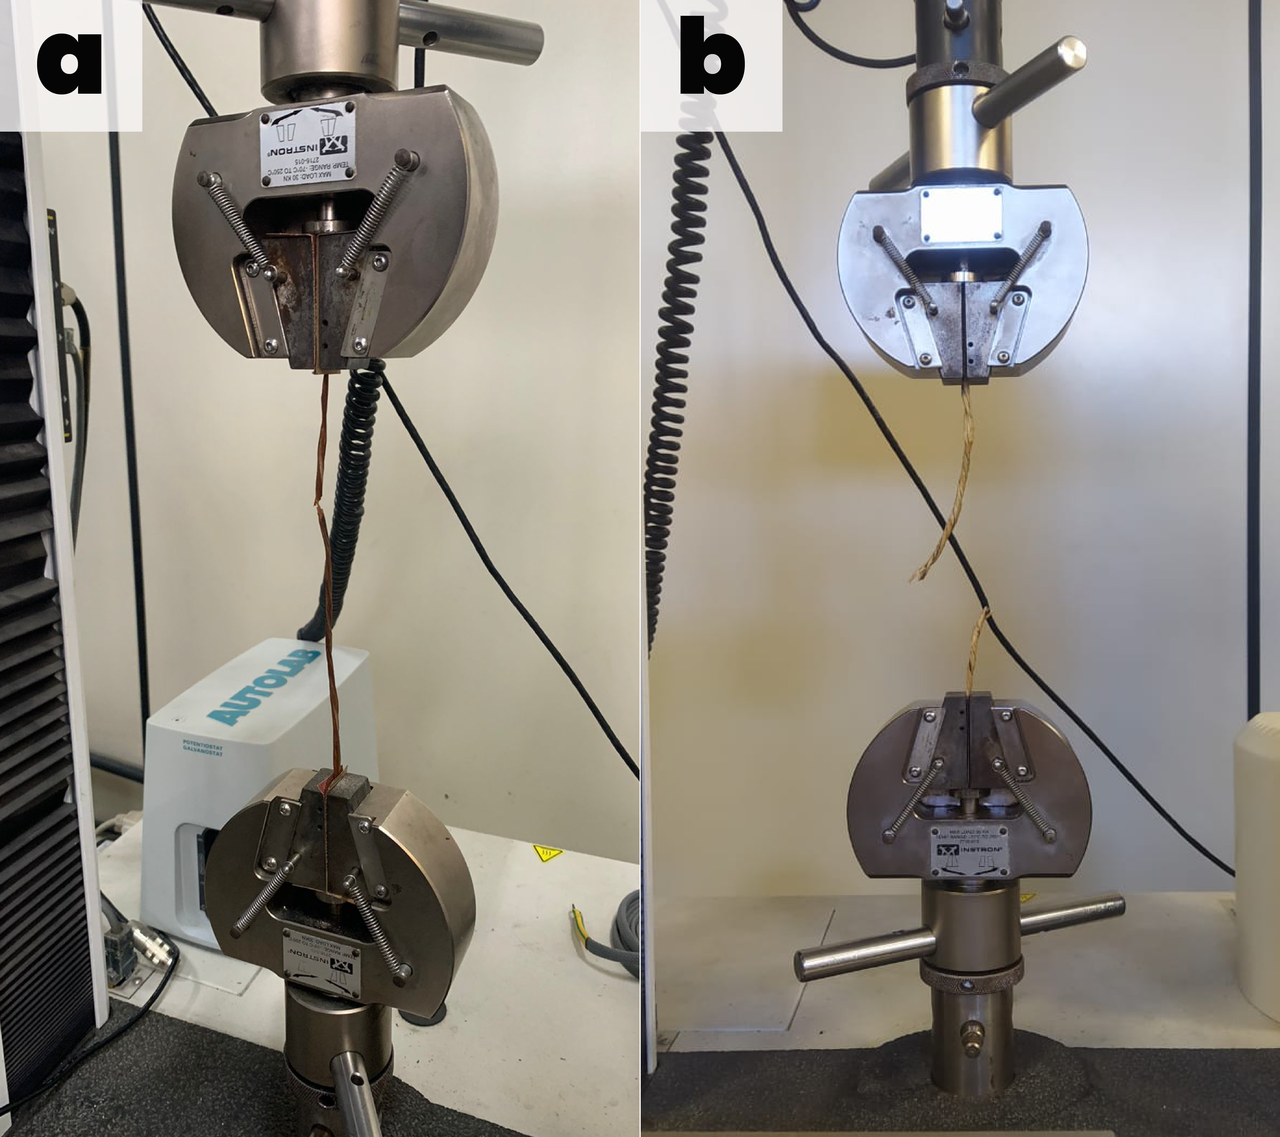
\includegraphics[keepaspectratio]{capitulos/../img/maquina_ensaio.png}}

}

\caption{\label{fig-maquina}Máquina universal de ensaios --- equipamento
para medição de resistência à tração e perfuração dos geotêxteis
conforme normas ABNT e ASTM.}

\end{figure}%

\end{minipage}%
%
\begin{minipage}{0.50\linewidth}

\begin{figure}[H]

\centering{

\pandocbounded{
\includegraphics[keepaspectratio]{capitulos/../img/camara_degradacao.png}}

}

\caption{\label{fig-camara}Câmara de degradação acelerada --- simulação
de envelhecimento UV e intempéries para avaliar durabilidade em
condições de exposição contínua.}

\end{figure}%

\end{minipage}%

\end{figure}%

\subsection{Por Processo de
Fabricação}\label{por-processo-de-fabricauxe7uxe3o}

Os geotêxteis tecidos são fabricados pelo entrelaçamento de fibras em
trama regular (urdume e trama), produzidos em máquinas de tecelagem
industrial. Essa estrutura ordenada confere alta resistência à tração em
uma ou duas direções (dependendo da distribuição de fios), com
alongamento na ruptura relativamente baixo (10--30\%), o que os torna
adequados para aplicações de reforço de solo e contenção onde
deformações excessivas são indesejáveis. Os geotêxteis não tecidos, por
sua vez, são compostos por fibras dispostas aleatoriamente e unidas por
agulhamento mecânico, termofusão ou ligação química. A disposição
aleatória das fibras confere alta permeabilidade em todas as direções,
deformabilidade elevada (alongamento de 50--100\%+) e distribuição
uniforme de poros, características que os tornam ideais para funções de
filtração, drenagem e proteção de geomembranas.

\subsection{Por Matéria-Prima}\label{por-matuxe9ria-prima}

Os geotêxteis sintéticos são fabricados a partir de polímeros derivados
do petróleo, principalmente polipropileno (PP), poliéster (PET) e
polietileno (PE), com durabilidade de 50--100+ anos em condições de
aterramento (ausência de UV). Os geotêxteis naturais (ou biogeotêxteis)
são fabricados a partir de fibras vegetais como coco, juta, sisal e
taboa (\emph{Typha}), com tempo de biodegradação de 1--5 anos conforme a
fibra e as condições ambientais (ver \textbf{?@sec-biotexteis}). A
biodegradabilidade não é uma desvantagem, mas uma característica de
projeto: em aplicações de controle de erosão, o geotêxtil deve durar
apenas o tempo necessário para o estabelecimento da cobertura vegetal
(tipicamente 6--24 meses), após o qual a vegetação assume a função
protetora e o material se incorpora ao solo como matéria orgânica.

\section{Funções Geotécnicas}\label{funuxe7uxf5es-geotuxe9cnicas}

A Tabela~\ref{tbl-funcoes} sintetiza as seis funções geotécnicas que os
geotêxteis podem desempenhar, com o mecanismo físico envolvido e a
aplicação correspondente em bioengenharia de solos. Em muitas situações
de campo, um único geotêxtil desempenha duas ou mais funções
simultaneamente (por exemplo, filtração + separação na base de
enrocamento vegetado, conforme \textbf{?@sec-enrocamento}).

\begin{longtable}[]{@{}
  >{\raggedright\arraybackslash}p{(\linewidth - 4\tabcolsep) * \real{0.1739}}
  >{\raggedright\arraybackslash}p{(\linewidth - 4\tabcolsep) * \real{0.2391}}
  >{\raggedright\arraybackslash}p{(\linewidth - 4\tabcolsep) * \real{0.5870}}@{}}
\caption{Funções geotécnicas de geotêxteis e suas aplicações em
bioengenharia.}\label{tbl-funcoes}\tabularnewline
\toprule\noalign{}
\begin{minipage}[b]{\linewidth}\raggedright
Função
\end{minipage} & \begin{minipage}[b]{\linewidth}\raggedright
Mecanismo
\end{minipage} & \begin{minipage}[b]{\linewidth}\raggedright
Aplicação na bioengenharia
\end{minipage} \\
\midrule\noalign{}
\endfirsthead
\toprule\noalign{}
\begin{minipage}[b]{\linewidth}\raggedright
Função
\end{minipage} & \begin{minipage}[b]{\linewidth}\raggedright
Mecanismo
\end{minipage} & \begin{minipage}[b]{\linewidth}\raggedright
Aplicação na bioengenharia
\end{minipage} \\
\midrule\noalign{}
\endhead
\bottomrule\noalign{}
\endlastfoot
Filtração & Reter partículas de solo, permitir passagem de água &
Drenos, base de enrocamento, interface solo-pedra \\
Separação & Impedir mistura de camadas granulometricamente distintas &
Interface solo-brita em canaletas verdes
(\textbf{?@sec-canaleta-verde}) \\
Reforço & Resistir a esforços de tração no interior do solo & Taludes
íngremes, solo reforçado em paredes Krainer
(\textbf{?@sec-parede-krainer}) \\
Proteção & Absorver energia de impacto & Proteção de geomembranas em
aterros \\
Drenagem & Conduzir fluidos no plano do geotêxtil & Geodrenos verticais
e horizontais \\
Controle de erosão & Cobrir e proteger superfície exposta & Biomantas
(\textbf{?@sec-biomantas}), TRM \\
\end{longtable}

\section{Propriedades}\label{propriedades}

\subsection{Mecânicas}\label{mecuxe2nicas}

As propriedades mecânicas fundamentais determinam o desempenho
estrutural do geotêxtil e incluem a resistência à tração (kN/m, medida
pelo ensaio de faixa larga conforme ABNT NBR 12824, que aplica carga
distribuída em uma amostra de 200 mm de largura até a ruptura), o
alongamento na ruptura (\% de deformação máxima antes da ruptura,
indicador da ductilidade do material), a resistência ao puncionamento
(kN, medida pelo ensaio CBR conforme ABNT NBR 13359, que simula a
perfuração por pedras pontiagudas ou raízes) e a resistência ao rasgo
(kN, ensaio trapezoidal que avalia a propagação de rasgos a partir de
defeitos pré-existentes).

\subsection{Hidráulicas}\label{hidruxe1ulicas}

As propriedades hidráulicas determinam o comportamento do geotêxtil como
filtro e dreno, e compreendem a permissividade (\(\psi\), s⁻¹), que
indica a capacidade de fluxo perpendicular ao plano do geotêxtil (vazão
por unidade de área sob gradiente hidráulico unitário), a
transmissividade (\(\theta\), m²/s), que mede a capacidade de fluxo no
plano do geotêxtil (relevante para funções de drenagem), e a abertura de
filtração (\(O_{95}\), mm), que define o diâmetro da partícula
correspondente ao percentil de 95\% da distribuição de tamanhos de poros
(indica a maior partícula que pode passar através do geotêxtil).

\subsection{Critério de Filtração}\label{crituxe9rio-de-filtrauxe7uxe3o}

Para que o geotêxtil desempenhe adequadamente a função de filtro sem
colmatar (entupir com partículas finas) nem permitir a passagem
excessiva de solo (piping interno), a abertura de filtração deve
satisfazer simultaneamente dois critérios de projeto

\[
O_{95} < (2 \text{ a } 3) \cdot D_{85,solo}
\]

que garante a retenção das partículas de solo (critério de retenção), e

\[
O_{95} > (1 \text{ a } 2) \cdot D_{15,solo}
\]

que garante a passagem de água sem acúmulo de poropressões (critério de
permeabilidade). Os parâmetros \(D_{85}\) e \(D_{15}\) referem-se aos
diâmetros correspondentes a 85\% e 15\% da curva granulométrica do solo
adjacente, respectivamente.

\section{Geotêxteis no Baixo São
Francisco}\label{geotuxeaxteis-no-baixo-suxe3o-francisco}

A experiência de campo no Baixo São Francisco constitui um dos estudos
de caso mais abrangentes sobre biogeotêxteis em ambiente tropical no
Brasil. A aplicação de biotêxteis de fibras de coco, juta e sisal na
proteção de taludes marginais do rio São Francisco em Sergipe e Alagoas,
monitorada ao longo de múltiplos ciclos hidrológicos, demonstrou
resultados expressivos. A Figura~\ref{fig-coleta} apresenta a coleta de
dados em campo, ilustrando o protocolo de monitoramento da performance
dos geotêxteis em taludes marginais sujeitos à variação de nível do rio.
Os resultados indicaram redução de 90--95\% na perda de solo no primeiro
ano de instalação, cobertura vegetal superior a 80\% em 90 dias sob
biomantas de fibra de coco, biodegradação controlada em 2--5 anos
(período suficiente para o pleno estabelecimento vegetal) e custo
40--60\% inferior ao gabião metálico para a mesma extensão protegida.

\begin{figure}

\centering{


\includegraphics[width=0.8\linewidth,height=\textheight,keepaspectratio]{capitulos/../img/coleta_campo.png}

}

\caption{\label{fig-coleta}Coleta de dados em campo no Baixo São
Francisco --- monitoramento da performance dos geotêxteis em taludes
marginais do rio.}

\end{figure}%

\section{Ensaios Normatizados}\label{ensaios-normatizados}

A caracterização dos geotêxteis é regulamentada por normas técnicas da
ABNT (Brasil) e da ASTM (internacional), que definem os procedimentos de
ensaio, as dimensões dos corpos de prova e os critérios de aceitação. A
Tabela~\ref{tbl-ensaios} apresenta os ensaios fundamentais e as normas
correspondentes, que devem ser indicados na especificação técnica de
qualquer projeto de bioengenharia que empregue geotêxteis.

\begin{longtable}[]{@{}
  >{\raggedright\arraybackslash}p{(\linewidth - 6\tabcolsep) * \real{0.1633}}
  >{\raggedright\arraybackslash}p{(\linewidth - 6\tabcolsep) * \real{0.2245}}
  >{\raggedright\arraybackslash}p{(\linewidth - 6\tabcolsep) * \real{0.2245}}
  >{\raggedright\arraybackslash}p{(\linewidth - 6\tabcolsep) * \real{0.3878}}@{}}
\caption{Ensaios normatizados para
geotêxteis.}\label{tbl-ensaios}\tabularnewline
\toprule\noalign{}
\begin{minipage}[b]{\linewidth}\raggedright
Ensaio
\end{minipage} & \begin{minipage}[b]{\linewidth}\raggedright
Norma ABNT
\end{minipage} & \begin{minipage}[b]{\linewidth}\raggedright
Norma ASTM
\end{minipage} & \begin{minipage}[b]{\linewidth}\raggedright
Propriedade medida
\end{minipage} \\
\midrule\noalign{}
\endfirsthead
\toprule\noalign{}
\begin{minipage}[b]{\linewidth}\raggedright
Ensaio
\end{minipage} & \begin{minipage}[b]{\linewidth}\raggedright
Norma ABNT
\end{minipage} & \begin{minipage}[b]{\linewidth}\raggedright
Norma ASTM
\end{minipage} & \begin{minipage}[b]{\linewidth}\raggedright
Propriedade medida
\end{minipage} \\
\midrule\noalign{}
\endhead
\bottomrule\noalign{}
\endlastfoot
Tração faixa larga & NBR 12824 & D4595 & Resistência à tração e
alongamento \\
Puncionamento CBR & NBR 13359 & D6241 & Resistência à perfuração \\
Rasgo trapezoidal & NBR 15314 & D4533 & Resistência à propagação de
rasgo \\
Permissividade & NBR 15223 & D4491 & Capacidade de fluxo
perpendicular \\
Abertura de filtração & NBR 12956 & D4751 & Tamanho efetivo de poros \\
Massa por unidade de área & NBR 12568 & D5261 & Gramatura (g/m²) \\
\end{longtable}

\begin{tcolorbox}[enhanced jigsaw, leftrule=.75mm, colframe=quarto-callout-note-color-frame, colback=white, bottomrule=.15mm, opacityback=0, colbacktitle=quarto-callout-note-color!10!white, breakable, bottomtitle=1mm, opacitybacktitle=0.6, title=\textcolor{quarto-callout-note-color}{\faInfo}\hspace{0.5em}{Tendência}, titlerule=0mm, toprule=.15mm, toptitle=1mm, rightrule=.15mm, left=2mm, arc=.35mm, coltitle=black]

A substituição progressiva de geossintéticos sintéticos por naturais
(biogeotêxteis) em aplicações de controle de erosão é uma tendência
global alinhada com os princípios de economia circular e soluções
baseadas na natureza (ver \textbf{?@sec-nbs}). Em aplicações temporárias
(proteção de taludes durante o estabelecimento vegetal), a
biodegradabilidade do biogeotêxtil é uma vantagem funcional, não uma
limitação.

\end{tcolorbox}

\chapter{Biotêxteis}\label{biotuxeaxteis}

\# Biotêxteis de Fibras Vegetais \{\#sec-biotexteis\}

Os biotêxteis são geotêxteis fabricados exclusivamente a partir de
fibras vegetais, projetados para biodegradação controlada após o
cumprimento de sua função protetora. Enquanto os geotêxteis sintéticos
(ver \textbf{?@sec-geotexteis}) persistem no solo por décadas ou
séculos, os biotêxteis são dimensionados para durar apenas o tempo
necessário ao estabelecimento da cobertura vegetal (tipicamente 6--36
meses), após o qual se decompõem e se incorporam ao solo como matéria
orgânica, contribuindo para a ciclagem de nutrientes e a melhoria da
estrutura edáfica. Essa característica os posiciona como uma evolução
dos geotêxteis convencionais alinhada com os princípios de economia
circular e soluções baseadas na natureza (ver \textbf{?@sec-nbs}). A
Figura~\ref{fig-tear} mostra um tear utilizado na confecção artesanal de
biotêxteis, onde fibras vegetais são tramadas para produzir mantas com
abertura e gramatura controladas, enquanto a Figura~\ref{fig-junco}
apresenta a fibra de junco antes do processamento, ilustrando a
matéria-prima renovável e abundante que sustenta a produção desses
materiais.

\begin{figure}

\begin{minipage}{0.50\linewidth}

\begin{figure}[H]

\centering{

\pandocbounded{
\includegraphics[keepaspectratio]{capitulos/../img/tear_fibras.jpg}}

}

\caption{\label{fig-tear}Tear para confecção de biotêxteis --- fibras
vegetais sendo tramadas para produzir geotêxteis biodegradáveis com
abertura e gramatura controladas.}

\end{figure}%

\end{minipage}%
%
\begin{minipage}{0.50\linewidth}

\begin{figure}[H]

\centering{

\pandocbounded{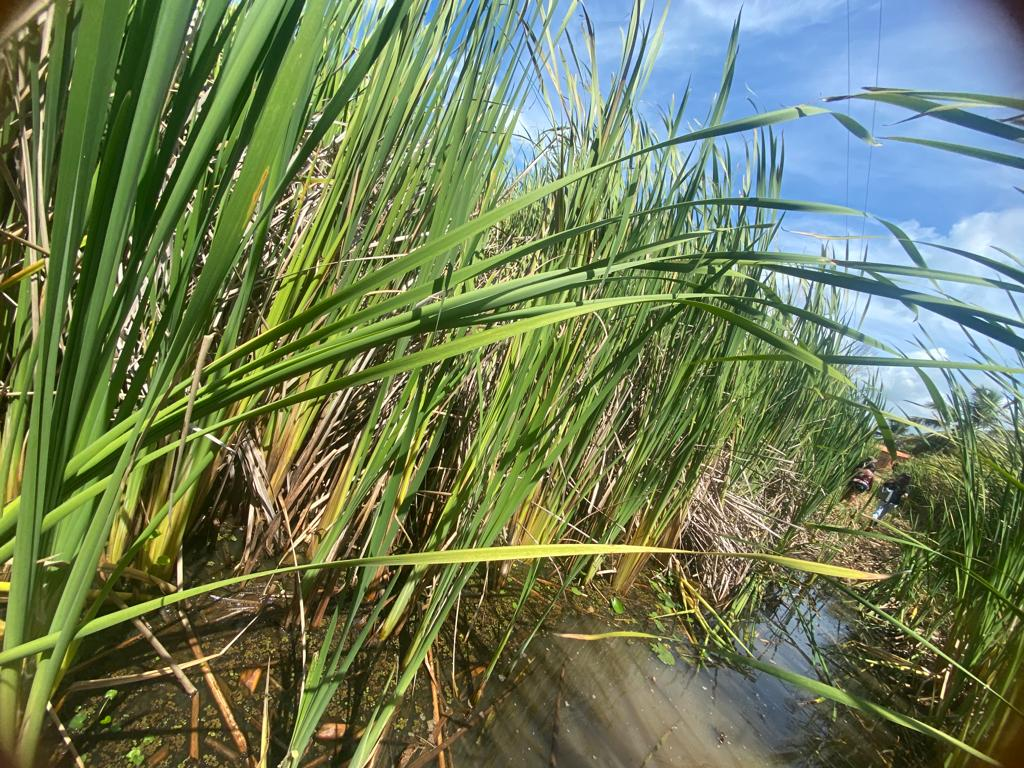
\includegraphics[keepaspectratio]{capitulos/../img/junco_fibra.jpg}}

}

\caption{\label{fig-junco}Fibra de junco utilizada na produção de
biotêxteis --- matéria-prima renovável e abundante disponível em regiões
tropicais.}

\end{figure}%

\end{minipage}%

\end{figure}%

\section{\texorpdfstring{Geotêxtil de Taboa (\emph{Typha
domingensis})}{Geotêxtil de Taboa (Typha domingensis)}}\label{geotuxeaxtil-de-taboa-typha-domingensis}

\subsection{Desenvolvimento}\label{desenvolvimento}

O geotêxtil tecido tipo \emph{geogrid} de taboa é uma inovação protegida
por patente INPI BR1020230222110 (concedida 2025), desenvolvida pelo
autor e colaboradores. A taboa (\emph{Typha domingensis} Pers.) é uma
macrófita aquática cosmopolita que coloniza áreas úmidas, várzeas e
margens de reservatórios em todo o território brasileiro, frequentemente
considerada planta invasora por sua capacidade de rápida proliferação
vegetativa. O aproveitamento de suas folhas fibrosas como matéria-prima
para biotêxteis transforma um passivo ambiental (biomassa invasora) em
insumo produtivo com valor agregado.

\subsection{Características}\label{caracteruxedsticas}

O geotêxtil de taboa é produzido a partir de folhas de \emph{Typha
domingensis} Pers., que são colhidas, secas e tramadas em padrão tela
simples (\emph{plain weave}) formando uma malha aberta tipo geogrid com
abertura ajustável de 10--30 mm. A abertura da malha é um parâmetro de
projeto definido em função da granulometria do solo a ser protegido e da
função desejada (aberturas menores para filtração, maiores para
intertravamento mecânico). A massa por área varia de 300 a 800 g/m²
(ajustável pela espessura e espaçamento das fibras), a resistência à
tração situa-se entre 2 e 8 kN/m (inferior aos sintéticos, mas adequada
para proteção superficial e reforço leve), e a biodegradação ocorre em
12--36 meses, controlável por tratamento com bioresinas que retardam a
decomposição sem comprometer a compostabilidade final.

\subsection{Mecanismo de
Intertravamento}\label{mecanismo-de-intertravamento}

O padrão geogrid (malha aberta com aberturas regulares) permite o
intertravamento mecânico com o solo, um mecanismo distinto da simples
cobertura proporcionada por biomantas (ver \textbf{?@sec-biomantas}). As
partículas de solo penetram nas aberturas da malha durante a compactação
ou sob a ação da chuva, criando um efeito de ancoragem que aumenta
significativamente a resistência ao cisalhamento na interface
solo-geotêxtil. Esse mecanismo é particularmente eficaz em taludes com
inclinação superior a 1V:2H, onde a gravidade tende a deslocar a camada
superficial de solo.

A resistência de interface pode ser estimada pela expressão

\[
\tau_{interface} = c_a + \sigma_n \cdot \tan \delta
\]

onde \(c_a\) é a adesão aparente na interface (kPa), \(\sigma_n\) é a
tensão normal atuante (kPa) e \(\delta\) é o ângulo de atrito de
interface, tipicamente correspondente a 0,7--0,9 vezes o ângulo de
atrito efetivo do solo (\(\phi'\)). O valor de \(\delta/\phi'\) depende
da rugosidade da fibra e do formato das aberturas, e deve ser
determinado experimentalmente por ensaio de cisalhamento direto em caixa
de cisalhamento de interface (ASTM D5321).

\subsection{Vantagens}\label{vantagens}

O geotêxtil de taboa apresenta um conjunto de vantagens que o posicionam
como alternativa competitiva aos geotêxteis de fibra de coco (padrão de
mercado para biotêxteis). A matéria-prima é abundante em todo o
território brasileiro (Typha coloniza áreas úmidas naturais e
antropizadas), e sua colheita regular funciona como controle biológico
de uma espécie invasora. O custo de produção é 50--70\% inferior ao dos
geotêxteis sintéticos equivalentes, com pegada de carbono negativa (a
planta sequestra CO₂ durante o crescimento e o material se decompõe sem
liberar microplásticos). A produção pode ser descentralizada em
comunidades rurais, gerando renda local e valorização de áreas úmidas
atualmente subutilizadas.

\section{Geocomposto Híbrido}\label{geocomposto-huxedbrido}

\subsection{Conceito do Geocomposto
Híbrido}\label{conceito-do-geocomposto-huxedbrido}

O geocomposto híbrido combina uma camada de manta de fibras vegetais
(coco, juta ou sisal) com uma malha de reforço de rami (\emph{Boehmeria
nivea}), criando um material com proteção superficial integrada
(interceptação de splash, retenção hídrica) e resistência mecânica
suficiente para aplicação em taludes íngremes. A estrutura sanduíche
aproveita as propriedades complementares de cada componente, como mostra
a Tabela~\ref{tbl-geocomposto}.

\subsection{Componentes}\label{componentes-1}

\begin{longtable}[]{@{}
  >{\raggedright\arraybackslash}p{(\linewidth - 4\tabcolsep) * \real{0.2162}}
  >{\raggedright\arraybackslash}p{(\linewidth - 4\tabcolsep) * \real{0.2703}}
  >{\raggedright\arraybackslash}p{(\linewidth - 4\tabcolsep) * \real{0.5135}}@{}}
\caption{Componentes do geocomposto híbrido e suas funções
específicas.}\label{tbl-geocomposto}\tabularnewline
\toprule\noalign{}
\begin{minipage}[b]{\linewidth}\raggedright
Camada
\end{minipage} & \begin{minipage}[b]{\linewidth}\raggedright
Material
\end{minipage} & \begin{minipage}[b]{\linewidth}\raggedright
Função específica
\end{minipage} \\
\midrule\noalign{}
\endfirsthead
\toprule\noalign{}
\begin{minipage}[b]{\linewidth}\raggedright
Camada
\end{minipage} & \begin{minipage}[b]{\linewidth}\raggedright
Material
\end{minipage} & \begin{minipage}[b]{\linewidth}\raggedright
Função específica
\end{minipage} \\
\midrule\noalign{}
\endhead
\bottomrule\noalign{}
\endlastfoot
Superior & Manta de fibra de coco (300--500 g/m²) & Proteção contra
impacto de gotas, retenção hídrica superficial \\
Intermediária & Malha de rami tecida (tela simples) & Reforço mecânico
(tração e rasgo) \\
Inferior & Manta de fibra de coco (200--400 g/m²) & Contato íntimo com o
solo, filtração de partículas finas \\
\end{longtable}

A malha de rami é o elemento estrutural crítico do geocomposto, pois o
rami (\emph{Boehmeria nivea}) possui a maior resistência à tração entre
as fibras vegetais (até 60 cN/tex), com elongação na ruptura de apenas
2--4\% (comportamento quase-rígido), tornando-o ideal para função de
reforço.

\subsection{Propriedades}\label{propriedades-1}

O geocomposto híbrido apresenta resistência à tração combinada de 5--15
kN/m (superior à de cada componente isolado, pelo efeito de compósito),
massa por área de 600--1.200 g/m² (ajustável pela gramatura de cada
camada), durabilidade de 24--48 meses (compatível com o período de
estabelecimento vegetal em condições tropicais) e retenção hídrica
superior a 200\% do peso seco (a camada de fibra de coco absorve e retém
água da chuva, liberando-a gradualmente para o solo e as raízes em
formação).

\section{Geodreno Vegetal
Biodegradável}\label{geodreno-vegetal-biodegraduxe1vel}

\subsection{Conceito do Geodreno
Vegetal}\label{conceito-do-geodreno-vegetal}

O geodreno vegetal é um dispositivo de drenagem subsuperficial fabricado
integralmente com materiais de origem vegetal, projetado para rebaixar
temporariamente o lençol freático em taludes e encostas instáveis
durante o período crítico de estabelecimento da vegetação.
Diferentemente dos geodrenos sintéticos (que permanecem indefinidamente
no solo), o geodreno vegetal se biodegrada em 18--36 meses, período após
o qual a drenagem é assumida pelos macroporos criados pelas raízes da
vegetação estabelecida.

\subsection{Estrutura}\label{estrutura}

O geodreno vegetal é composto por placas drenantes de fibras de taboa e
bananeira prensadas, cuja geometria interna em espinha-de-peixe
(\emph{herringbone}) cria canais preferenciais para a condução do fluxo
subsuperficial. O aglutinante utilizado é uma resina de mamona
(\emph{Ricinus communis}) com D-limoneno (solvente natural extraído de
cascas de citros), que confere rigidez estrutural sem comprometer a
biodegradabilidade. O envoltório externo consiste em geotêxtil não
tecido de fibra de coco, que funciona como filtro de proteção contra o
carreamento de partículas finas para o interior do dreno (colmatação).

\subsection{Desempenho}\label{desempenho}

O geodreno vegetal atinge vazão drenante de 0,5--2,0 L/(m·min) sob
gradiente hidráulico unitário (suficiente para rebaixamento localizado
em solos de permeabilidade média), resistência à compressão de 50--150
kPa (suporta a tensão geostática de 3--8 m de solo sobrejacente sem
colapso) e biodegradação controlável em 18--36 meses pela concentração
do aglutinante.

\begin{tcolorbox}[enhanced jigsaw, leftrule=.75mm, colframe=quarto-callout-note-color-frame, colback=white, bottomrule=.15mm, opacityback=0, colbacktitle=quarto-callout-note-color!10!white, breakable, bottomtitle=1mm, opacitybacktitle=0.6, title=\textcolor{quarto-callout-note-color}{\faInfo}\hspace{0.5em}{Patentes relacionadas}, titlerule=0mm, toprule=.15mm, toptitle=1mm, rightrule=.15mm, left=2mm, arc=.35mm, coltitle=black]

As inovações biotecnológicas apresentadas neste capítulo incluem o
geotêxtil de taboa (BR1020230222110, concedida 2025), o geocomposto
híbrido (pedido depositado) e o geodreno vegetal (pedido depositado),
representando contribuições nacionais ao avanço dos biomateriais
aplicados à bioengenharia de solos.

\end{tcolorbox}

\section{Comparativo de Desempenho}\label{comparativo-de-desempenho}

A Tabela~\ref{tbl-comparativo} confronta as propriedades dos biotêxteis
(coco e taboa) com as de um geotêxtil sintético de polipropileno (PP),
evidenciando os compromissos de projeto entre desempenho mecânico e
sustentabilidade ambiental. Os biotêxteis apresentam resistência à
tração inferior, mas oferecem retenção hídrica elevada, biodegradação
controlada (sem acúmulo de resíduos), pegada de carbono negativa e custo
competitivo, vantagens decisivas em aplicações de controle de erosão com
horizonte temporal de 1--5 anos.

\begin{longtable}[]{@{}llll@{}}
\caption{Comparativo entre biotêxteis e geotêxtil sintético
(PP).}\label{tbl-comparativo}\tabularnewline
\toprule\noalign{}
Propriedade & Geotêxtil de coco & Geotêxtil de taboa & Geotêxtil PP \\
\midrule\noalign{}
\endfirsthead
\toprule\noalign{}
Propriedade & Geotêxtil de coco & Geotêxtil de taboa & Geotêxtil PP \\
\midrule\noalign{}
\endhead
\bottomrule\noalign{}
\endlastfoot
Custo (R\$/m²) & 8--15 & 5--12 & 10--25 \\
Biodegradação & 2--4 anos & 1--3 anos & \textgreater{} 100 anos \\
Resistência tração (kN/m) & 3--8 & 2--8 & 5--50 \\
Retenção hídrica & Alta & Muito alta & Baixa \\
Pegada CO₂ & Negativa & Negativa & Positiva \\
Reciclabilidade & Compostável & Compostável & Reciclável \\
\end{longtable}

\chapter{Biopolímeros
Superabsorventes}\label{biopoluxedmeros-superabsorventes}

\# Biopolímeros Superabsorventes \{\#sec-biopolimeros\}

Os biopolímeros superabsorventes (Bio-SAP, do inglês
\emph{Superabsorbent Biopolymer}) são materiais de origem vegetal
capazes de absorver e reter grandes volumes de água (100--500 vezes seu
peso seco), liberando-a gradualmente para a zona radicular das plantas à
medida que o potencial matricial do solo diminui por evapotranspiração.
Diferentemente dos hidrogéis sintéticos (poliacrilatos de sódio), os
Bio-SAPs são integralmente biodegradáveis e não geram resíduos de
microplásticos no solo. Essa característica os torna especialmente
relevantes para aplicações de bioengenharia de solos em regiões
semiáridas, onde o déficit hídrico no período pós-plantio é o principal
fator de mortalidade de mudas em taludes recuperados. A
Figura~\ref{fig-taboa} mostra o material vegetal de taboa (\emph{Typha
domingensis}) que constitui a matéria-prima do Bio-SAP, cuja polpa
celulósica é processada quimicamente para adquirir propriedades
superabsorventes.

\begin{figure}

\centering{

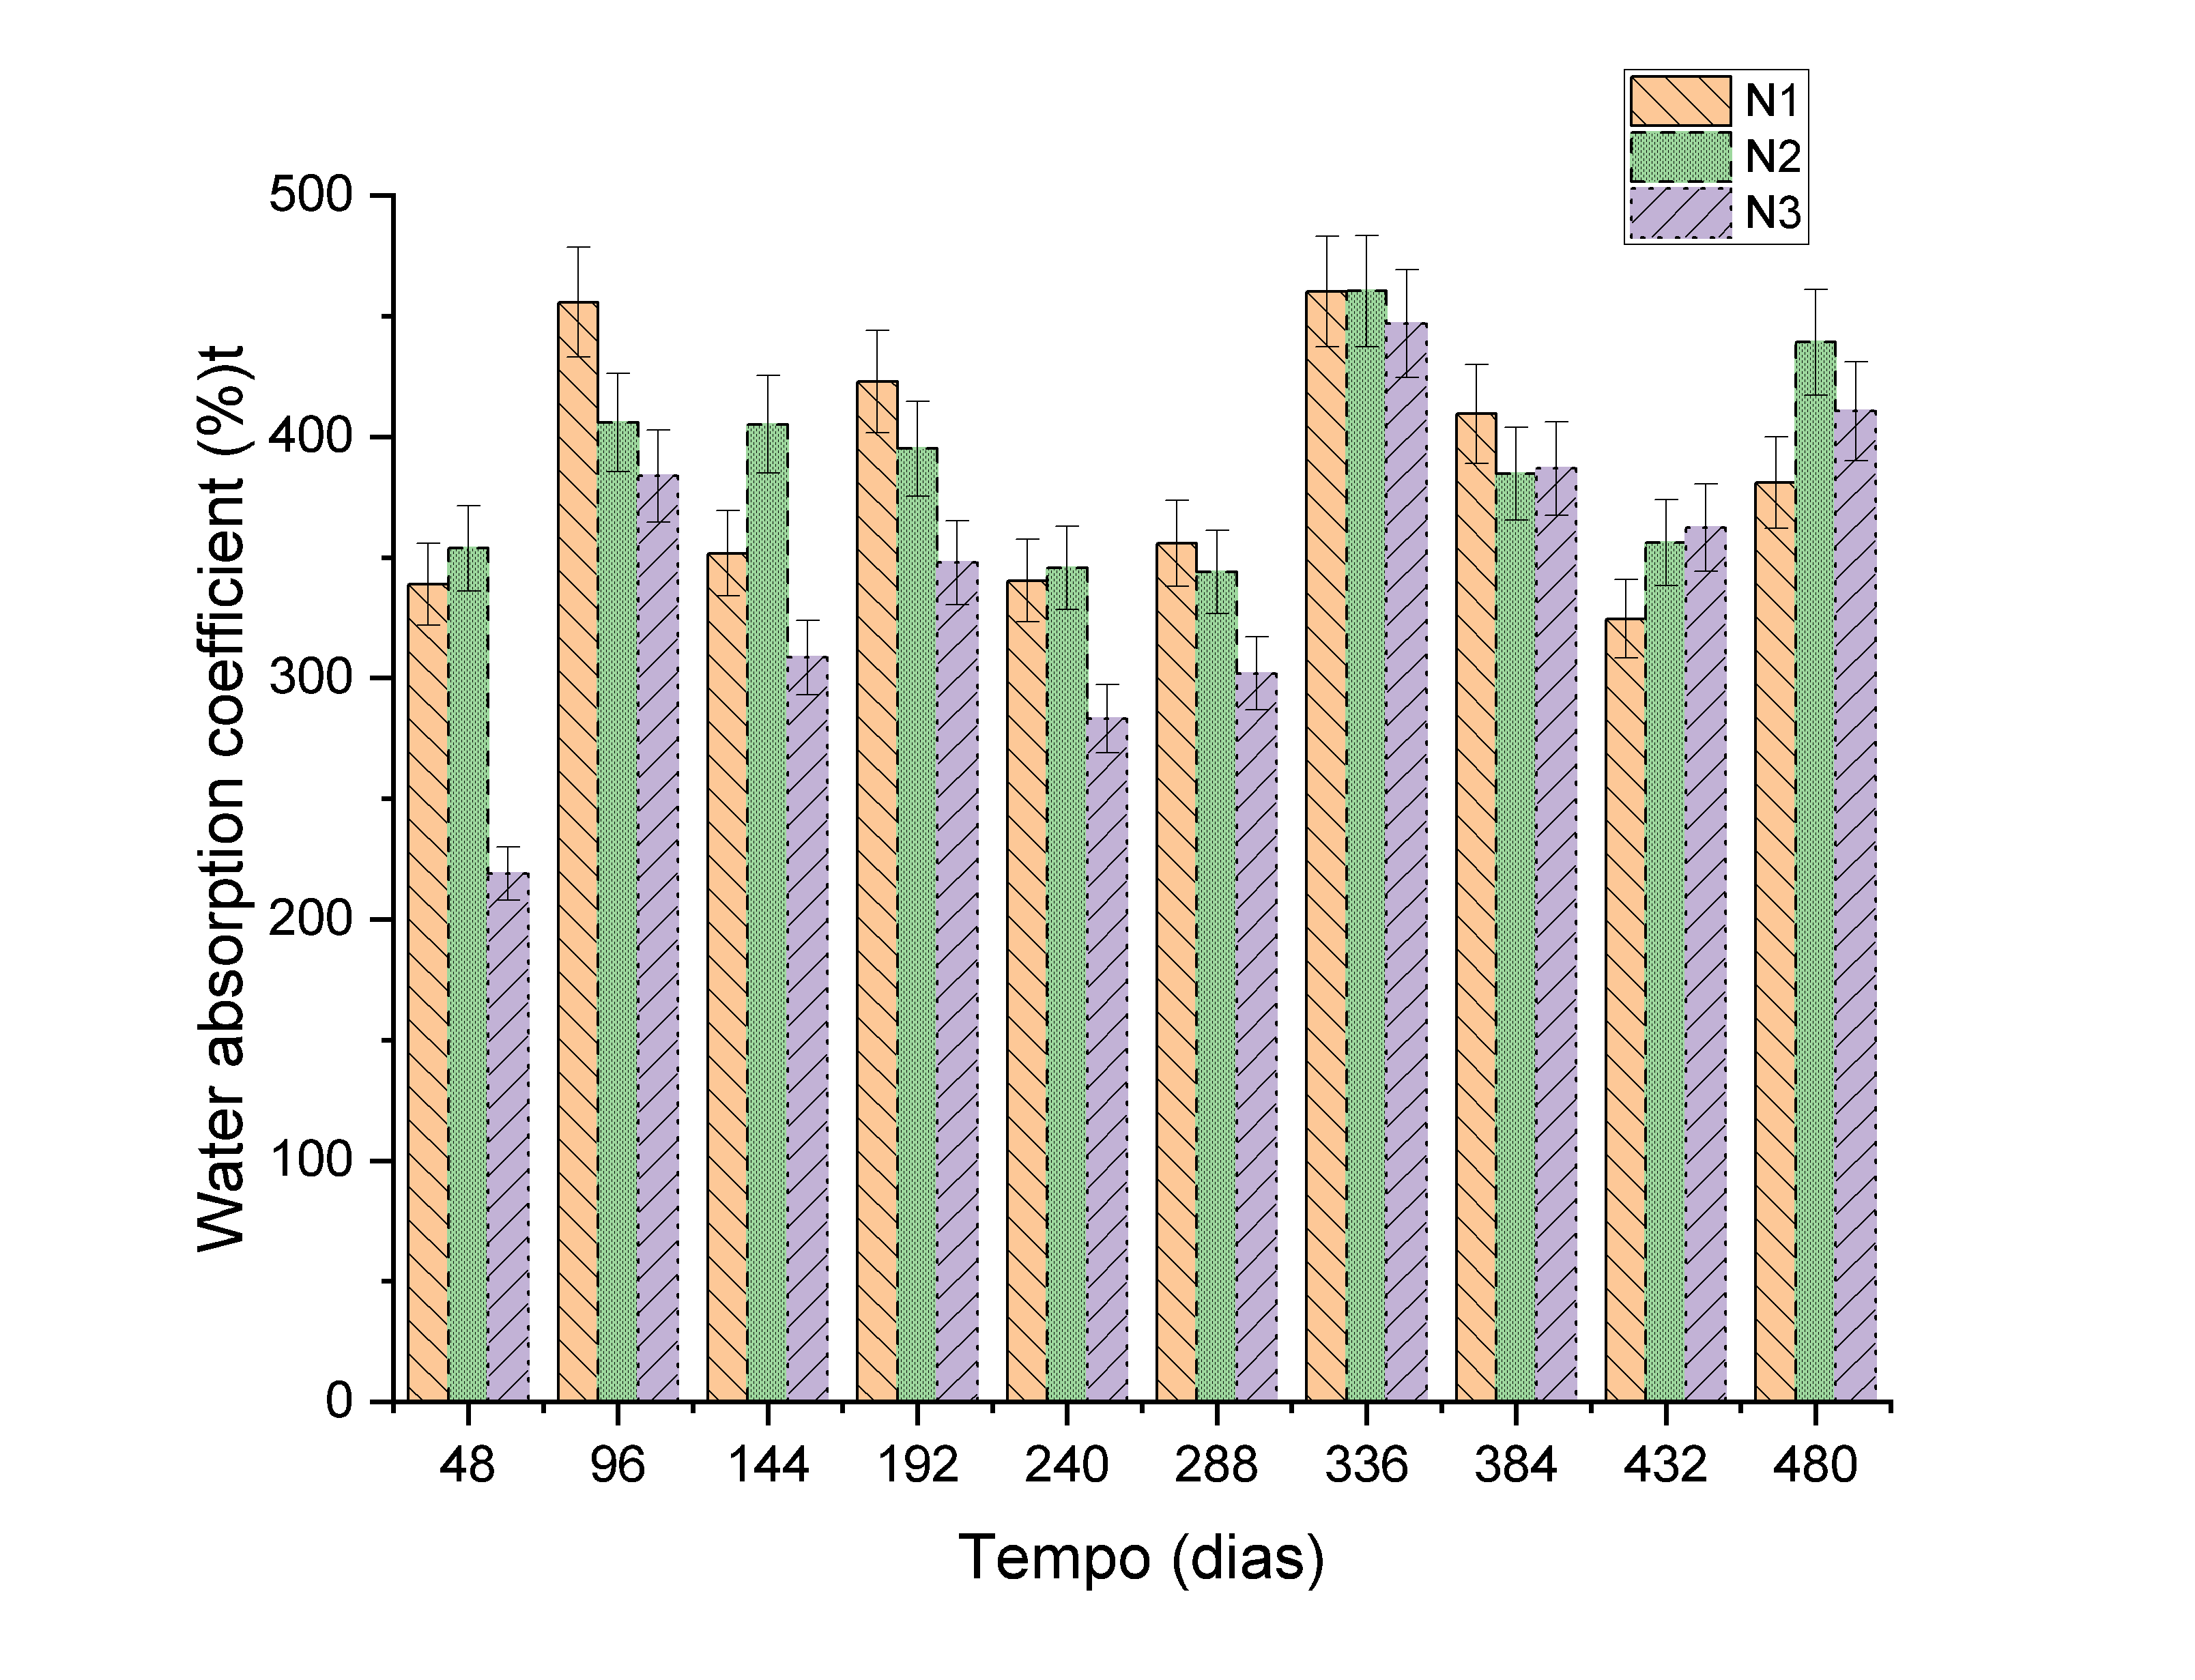
\includegraphics[width=0.8\linewidth,height=\textheight,keepaspectratio]{capitulos/../img/taboa_material.png}

}

\caption{\label{fig-taboa}Material de taboa (\emph{Typha domingensis})
utilizado na produção do Bio-SAP --- polpa celulósica das folhas
processada quimicamente para conferir propriedades superabsorventes.}

\end{figure}%

\section{Bio-SAP de Taboa}\label{bio-sap-de-taboa}

\subsection{Desenvolvimento}\label{desenvolvimento-1}

O Bio-SAP de taboa (\emph{Typha domingensis}) é uma inovação
desenvolvida a partir da polpa celulósica da planta, processada por duas
reações químicas sequenciais (carboximetilação e reticulação) que
modificam a estrutura molecular da celulose, conferindo-lhe a capacidade
de formar hidrogéis com elevada retenção hídrica. A celulose nativa
possui grupos hidroxila (-OH) que atraem moléculas de água por ligações
de hidrogênio, mas a capacidade de absorção é limitada. A
carboximetilação substitui parte desses grupos hidroxila por grupos
carboximetila (-CH₂COONa), que são aniônicos em solução aquosa e criam
pressão osmótica no interior da rede polimérica, atraindo grandes
volumes de água. A reticulação subsequente (com epicloridrina) cria
ligações covalentes entre as cadeias de celulose, formando uma rede
tridimensional que impede a dissolução do material e confere
elasticidade mecânica.

\subsection{Processo de Produção}\label{processo-de-produuxe7uxe3o}

O fluxograma abaixo sintetiza as etapas de produção do Bio-SAP, desde a
colheita da taboa em campo até a obtenção do produto granulado pronto
para aplicação.


\includegraphics[width=7in,height=3.5in]{capitulos/19-biopolimeros_files/figure-latex/dot-figure-1.png}

\subsection{Propriedades}\label{propriedades-2}

A microestrutura do Bio-SAP pode ser observada na Figura~\ref{fig-mev},
que apresenta imagens de microscopia eletrônica de varredura (MEV)
comparando o material antes e após a absorção de água. No estado seco, o
Bio-SAP exibe uma superfície rugosa e compacta com microporos
colapsados; após a absorção, a estrutura se expande dramaticamente,
revelando uma rede tridimensional de poros interconectados que retêm a
água por capilaridade e pressão osmótica. A Tabela~\ref{tbl-biosap}
quantifica as principais propriedades do material.

\begin{figure}

\centering{

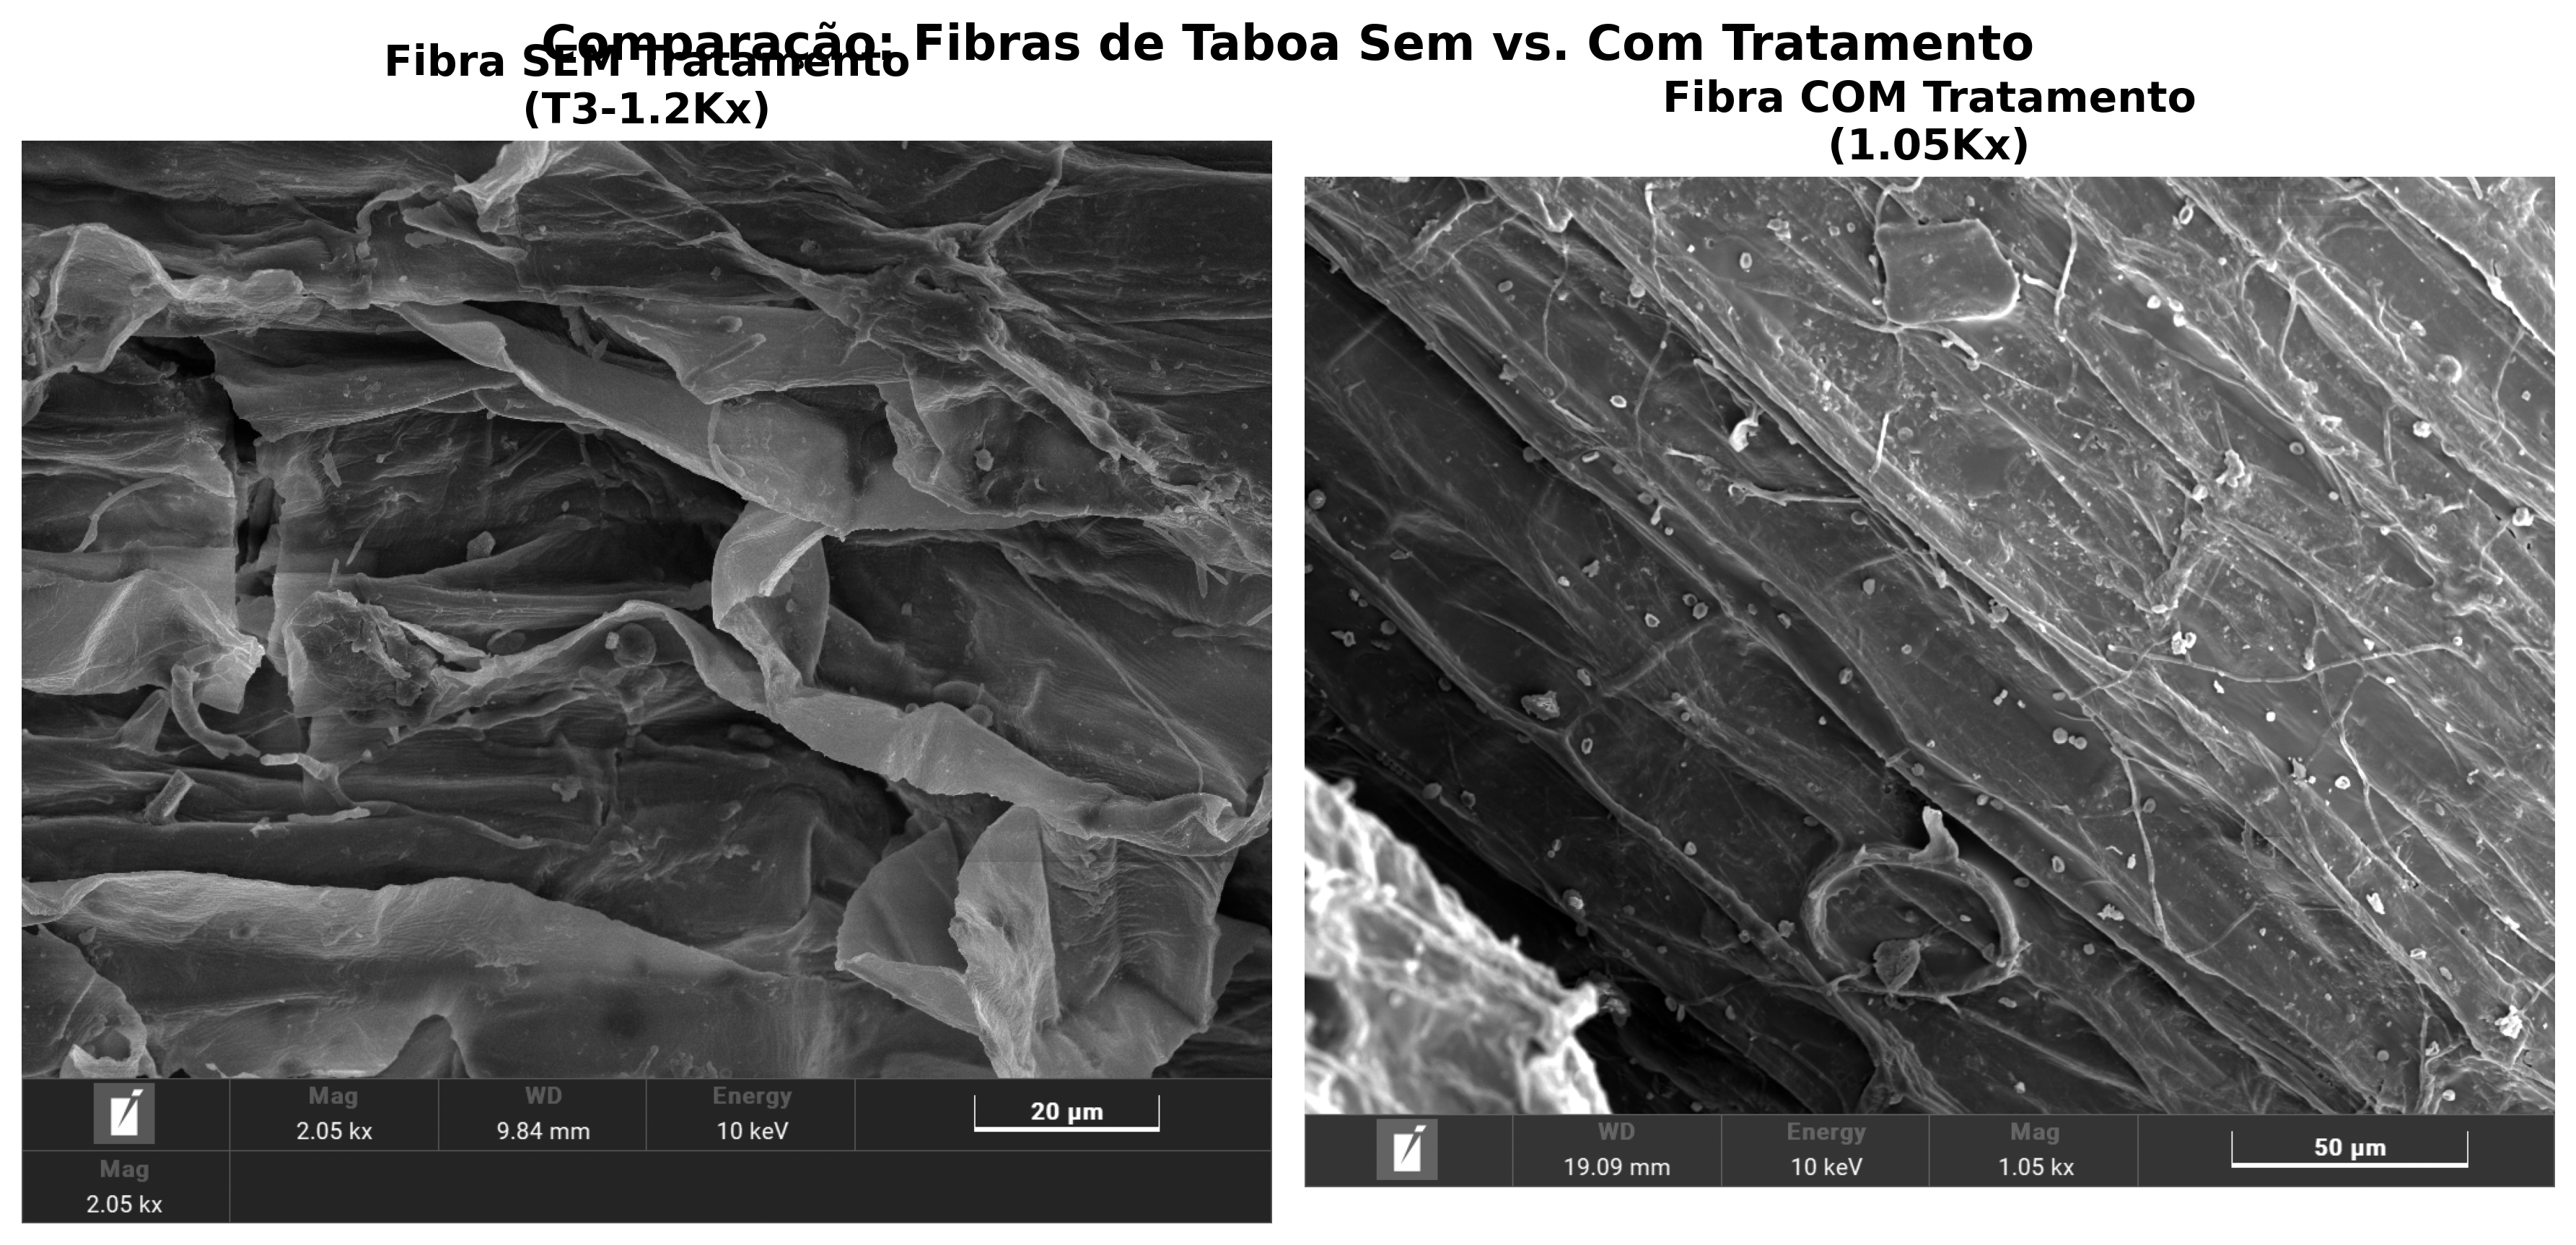
\includegraphics[width=0.8\linewidth,height=\textheight,keepaspectratio]{capitulos/../img/mev_comparacao.png}

}

\caption{\label{fig-mev}Microscopia eletrônica de varredura (MEV) do
Bio-SAP --- comparação da microestrutura antes (superfície compacta com
microporos colapsados) e após absorção de água (rede tridimensional
expandida).}

\end{figure}%

\begin{longtable}[]{@{}
  >{\raggedright\arraybackslash}p{(\linewidth - 4\tabcolsep) * \real{0.3171}}
  >{\raggedright\arraybackslash}p{(\linewidth - 4\tabcolsep) * \real{0.1707}}
  >{\raggedright\arraybackslash}p{(\linewidth - 4\tabcolsep) * \real{0.5122}}@{}}
\caption{Propriedades do Bio-SAP de
taboa.}\label{tbl-biosap}\tabularnewline
\toprule\noalign{}
\begin{minipage}[b]{\linewidth}\raggedright
Propriedade
\end{minipage} & \begin{minipage}[b]{\linewidth}\raggedright
Valor
\end{minipage} & \begin{minipage}[b]{\linewidth}\raggedright
Significado prático
\end{minipage} \\
\midrule\noalign{}
\endfirsthead
\toprule\noalign{}
\begin{minipage}[b]{\linewidth}\raggedright
Propriedade
\end{minipage} & \begin{minipage}[b]{\linewidth}\raggedright
Valor
\end{minipage} & \begin{minipage}[b]{\linewidth}\raggedright
Significado prático
\end{minipage} \\
\midrule\noalign{}
\endhead
\bottomrule\noalign{}
\endlastfoot
Capacidade de absorção em água destilada & 300--500 g/g & 1 kg de
Bio-SAP retém 300--500 L de água \\
Capacidade de absorção em solo & 150--250 g/g & Reduzida pela presença
de sais e finos \\
Tempo de absorção (90\%) & 15--30 min & Resposta rápida a eventos de
chuva \\
Taxa de liberação (50\%) & 12--48 h & Liberação gradual compatível com
demanda radicular \\
Biodegradação completa & 6--18 meses & Não deixa resíduos no solo \\
Granulometria & 0,5--2,0 mm & Compatível com mistura em substrato \\
\end{longtable}

\section{Geocompostos Hidrorretentores
Typha-Rami}\label{geocompostos-hidrorretentores-typha-rami}

\subsection{Conceito dos Geocompostos
Hidrorretentores}\label{conceito-dos-geocompostos-hidrorretentores}

Os geocompostos hidrorretentores integram o Bio-SAP em uma estrutura
sanduíche de biotêxtil (ver \textbf{?@sec-biotexteis}), criando um
sistema de retenção hídrica distribuída que pode ser instalado
diretamente sobre o talude como uma manta, eliminando a necessidade de
misturar manualmente o Bio-SAP ao solo. A Figura~\ref{fig-confeccao}
mostra o processo de confecção do geocomposto, onde o núcleo de Bio-SAP
é confinado entre duas camadas de biotêxtil de taboa-rami.

\begin{figure}

\centering{

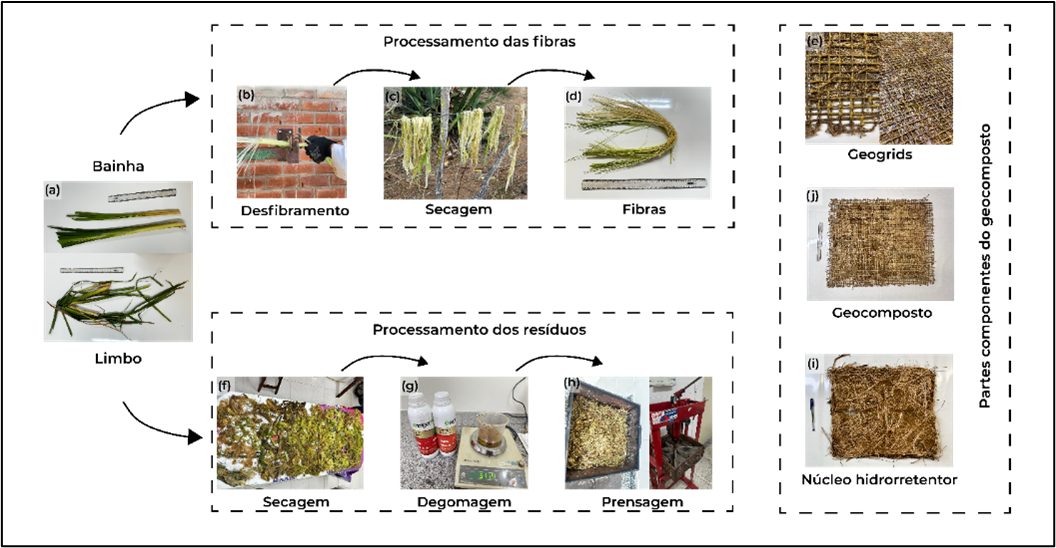
\includegraphics[width=0.8\linewidth,height=\textheight,keepaspectratio]{capitulos/../img/processo_confeccao.png}

}

\caption{\label{fig-confeccao}Processo de confecção do geocomposto
hidrorretentor --- estrutura sanduíche de biotêxtil de taboa-rami com
núcleo de Bio-SAP confinado entre as camadas.}

\end{figure}%

\subsection{Estrutura}\label{estrutura-1}

A Tabela~\ref{tbl-geocomposto-hidro} detalha os componentes da estrutura
sanduíche, onde cada camada desempenha uma função específica e
complementar.

\begin{longtable}[]{@{}
  >{\raggedright\arraybackslash}p{(\linewidth - 4\tabcolsep) * \real{0.3077}}
  >{\raggedright\arraybackslash}p{(\linewidth - 4\tabcolsep) * \real{0.3846}}
  >{\raggedright\arraybackslash}p{(\linewidth - 4\tabcolsep) * \real{0.3077}}@{}}
\caption{Estrutura do geocomposto hidrorretentor
Typha-Rami.}\label{tbl-geocomposto-hidro}\tabularnewline
\toprule\noalign{}
\begin{minipage}[b]{\linewidth}\raggedright
Camada
\end{minipage} & \begin{minipage}[b]{\linewidth}\raggedright
Material
\end{minipage} & \begin{minipage}[b]{\linewidth}\raggedright
Função
\end{minipage} \\
\midrule\noalign{}
\endfirsthead
\toprule\noalign{}
\begin{minipage}[b]{\linewidth}\raggedright
Camada
\end{minipage} & \begin{minipage}[b]{\linewidth}\raggedright
Material
\end{minipage} & \begin{minipage}[b]{\linewidth}\raggedright
Função
\end{minipage} \\
\midrule\noalign{}
\endhead
\bottomrule\noalign{}
\endlastfoot
Exterior (×2) & Biotêxtil de taboa-rami & Proteção mecânica, filtração e
reforço \\
Interior & Núcleo de Bio-SAP (300--800 g/m²) & Reservatório hídrico
distribuído \\
Aglutinante & \emph{Aloe vera} + amida 90\% & Fixação do Bio-SAP e
ativação da absorção \\
\end{longtable}

\subsection{Desempenho}\label{desempenho-1}

O geocomposto hidrorretentor apresenta WHC (\emph{Water Holding
Capacity}) superior a 300\% do peso seco, o que significa que cada m² de
geocomposto (com gramatura total de \textasciitilde1.500 g/m²) retém até
4,5 L de água, funcionando como um reservatório laminar distribuído
sobre toda a superfície do talude. A retenção de macronutrientes (N, P,
K) é superior a 60\%, reduzindo a lixiviação de fertilizantes aplicados
durante a revegetação. A integridade estrutural é mantida por pelo menos
180 dias em campo (período crítico de estabelecimento vegetal), e a
curva de retenção hídrica do geocomposto pode ser ajustada pela equação
de van Genuchten

\[
\theta(h) = \theta_r + \frac{\theta_s - \theta_r}{[1 + (\alpha \cdot h)^n]^m}
\]

onde \(\theta_r\) e \(\theta_s\) são os teores de água residual e
saturado (cm³/cm³), \(h\) é o potencial matricial (cm de coluna d'água),
e \(\alpha\) (cm⁻¹), \(n\) e \(m = 1 - 1/n\) são parâmetros de ajuste
que descrevem a forma da curva. A determinação desses parâmetros por
ajuste a dados experimentais permite prever a disponibilidade de água
para as plantas em função da tensão do solo, subsidiando o
dimensionamento da gramatura de Bio-SAP necessária para cada condição
climática.

\section{Aplicações}\label{aplicauxe7uxf5es-2}

A Figura~\ref{fig-alelopatia} apresenta ensaios de alelopatia e
germinação com Bio-SAP, demonstrando que o biopolímero não exerce efeito
inibitório sobre a germinação e o desenvolvimento de plântulas, condição
essencial para sua aplicação em projetos de revegetação.

\begin{figure}

\centering{

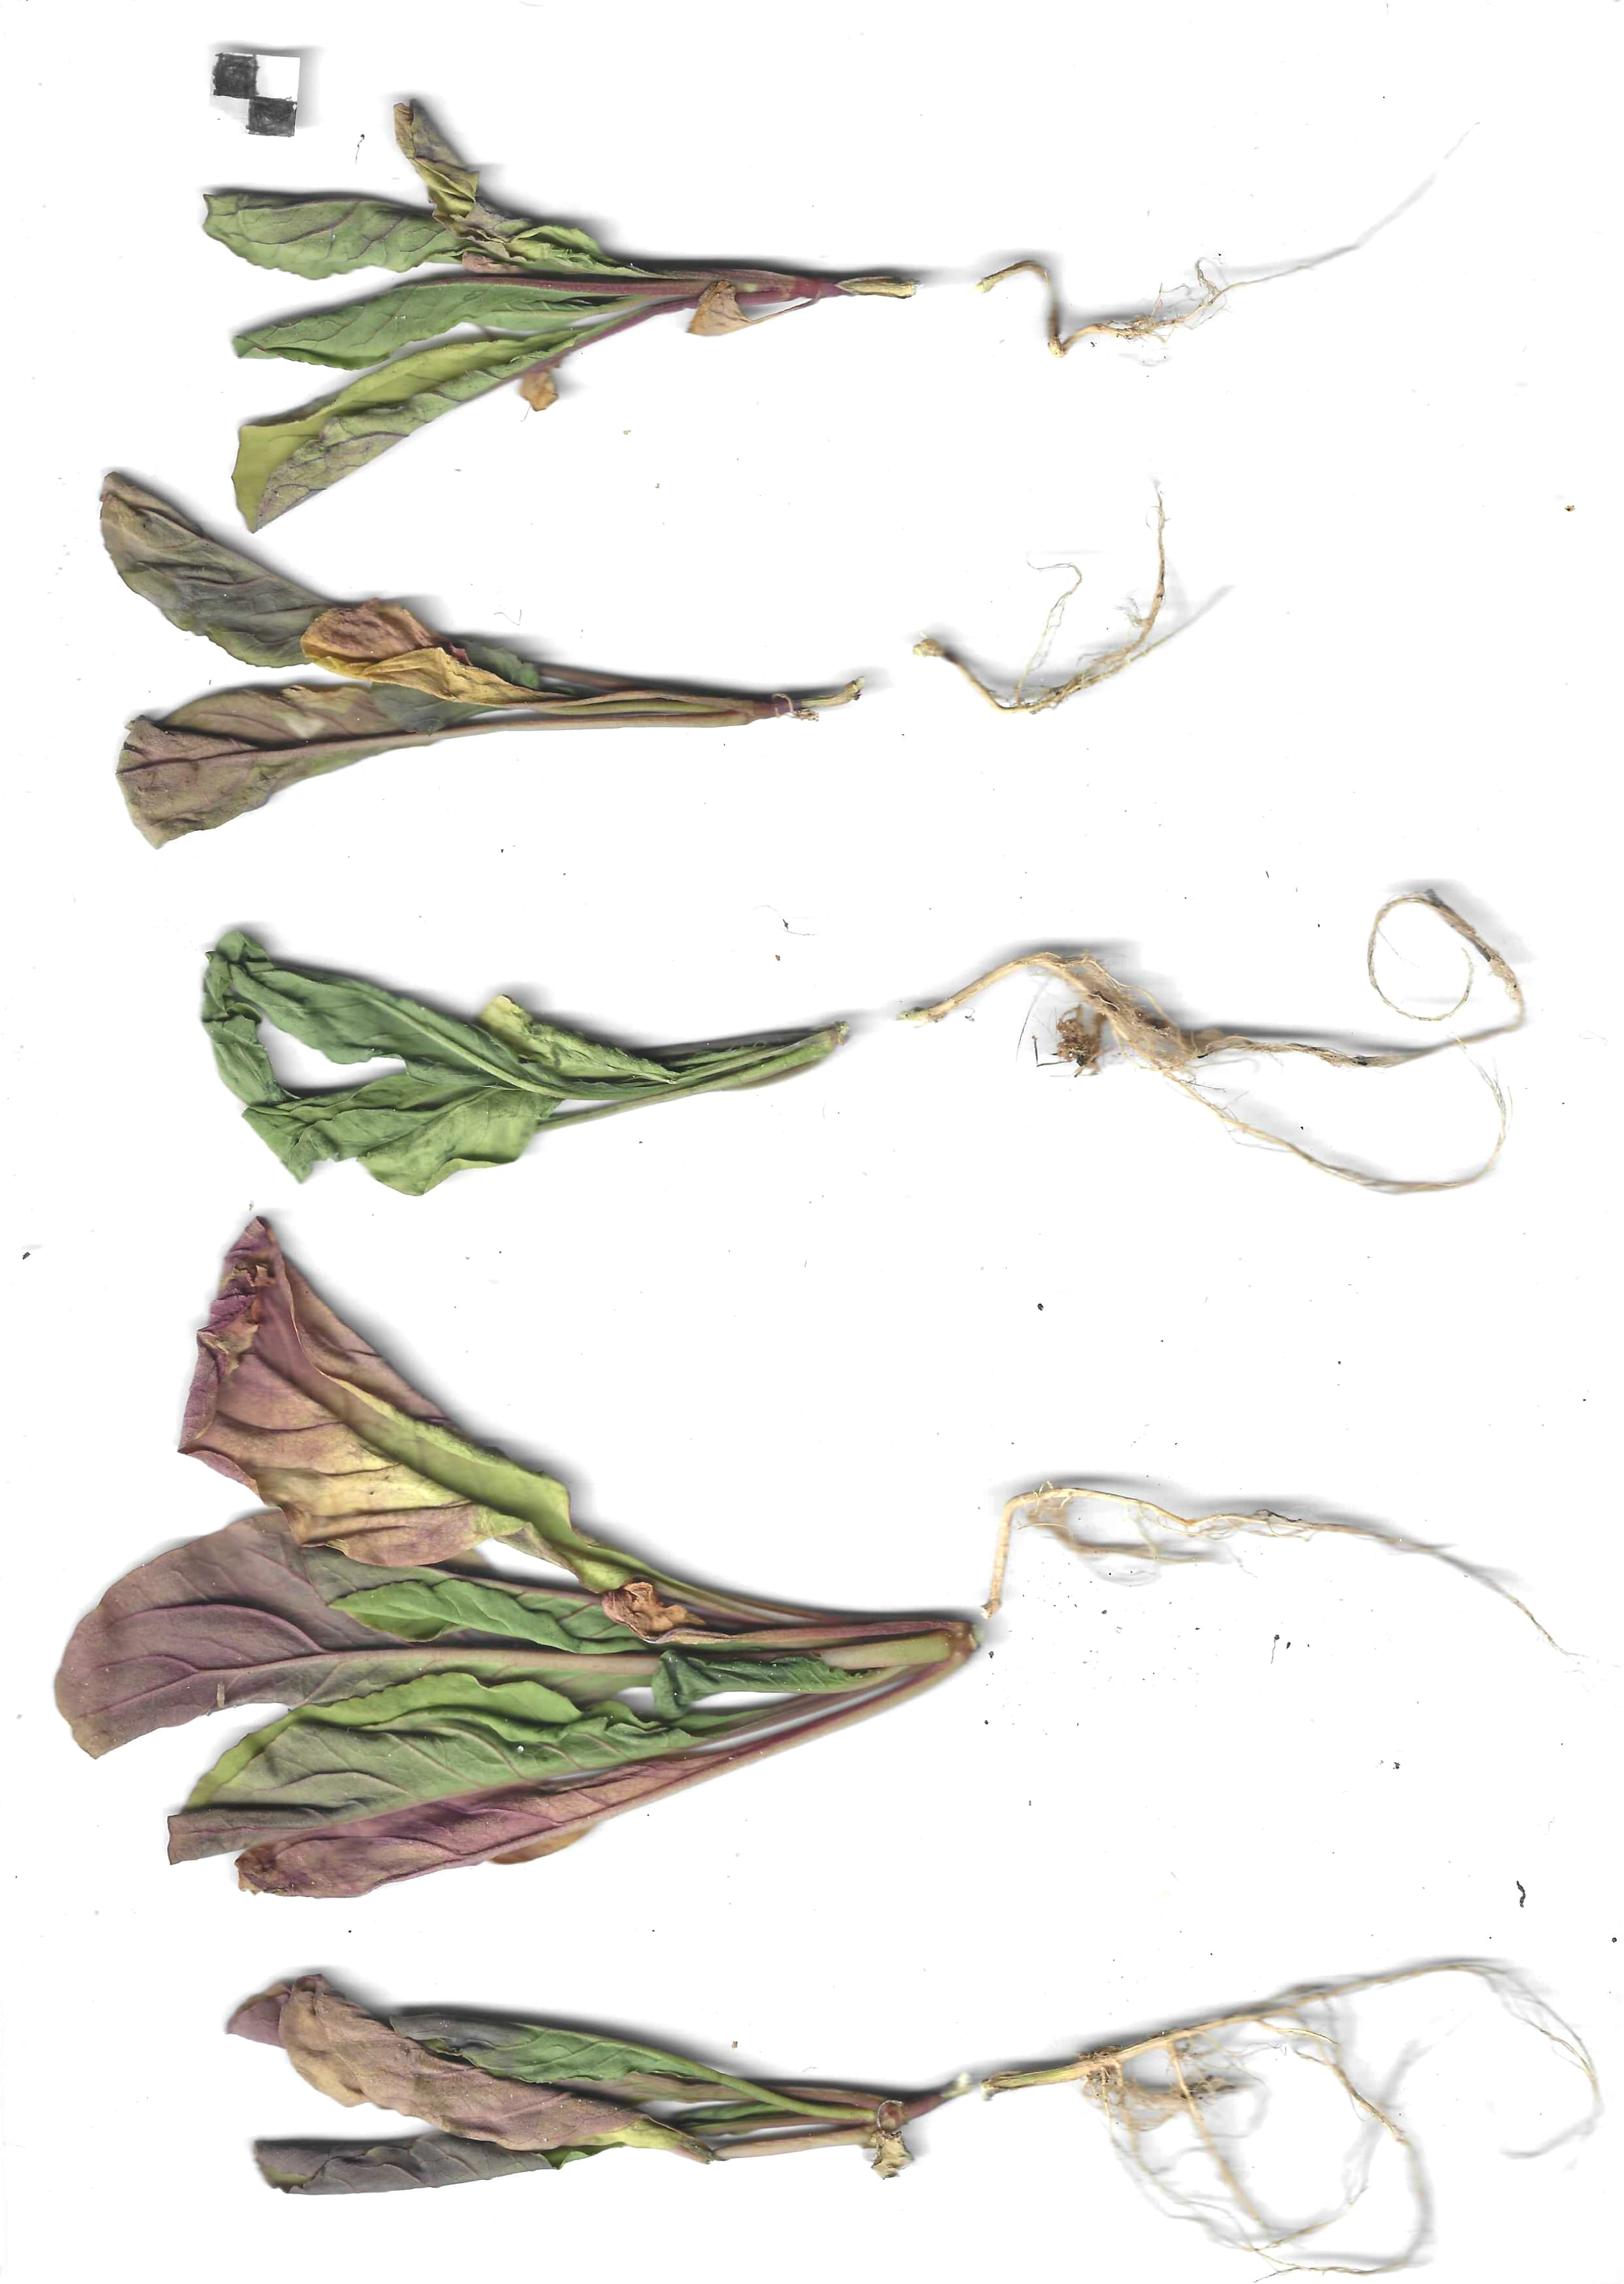
\includegraphics[width=0.75\linewidth,height=\textheight,keepaspectratio]{capitulos/../img/alelopatia_germinacao.jpg}

}

\caption{\label{fig-alelopatia}Ensaio de alelopatia e germinação com
Bio-SAP --- avaliação do efeito do biopolímero sobre o crescimento de
plântulas, demonstrando ausência de fitotoxicidade.}

\end{figure}%

Em projetos de recuperação de encostas, o Bio-SAP é instalado sob
biomantas (ver \textbf{?@sec-biomantas}) ou incorporado à pasta de
hidrossemeadura (ver \textbf{?@sec-hidrossemeadura}), retendo a água da
chuva na zona radicular e reduzindo a necessidade de irrigação em
50--70\% nos primeiros 90 dias, fator crítico em regiões semiáridas com
déficit hídrico prolongado. Na revegetação de taludes em áreas de
mineração, onde os substratos são altamente degradados (pH extremo,
ausência de matéria orgânica, baixa capacidade de retenção hídrica), a
combinação de Bio-SAP com composto orgânico cria condições mínimas para
o estabelecimento vegetal ao fornecer um reservatório hídrico e
nutricional que compensa as deficiências edáficas. Na produção de mudas
em viveiros, a incorporação de Bio-SAP ao substrato reduz a frequência
de irrigação em 40--60\% e aumenta a taxa de sobrevivência no
transplante para campo, reduzindo o estresse hídrico na fase de
adaptação.

\section{Vantagens sobre SAP
Sintéticos}\label{vantagens-sobre-sap-sintuxe9ticos}

A Tabela~\ref{tbl-comparativo-sap} confronta o Bio-SAP de taboa com os
SAPs sintéticos (poliacrilatos de sódio) que dominam o mercado atual,
evidenciando que o Bio-SAP oferece capacidade de absorção comparável
(300--500 g/g versus 300--600 g/g) com as vantagens decisivas de
biodegradabilidade total, ausência de microplásticos, matéria-prima
renovável e custo inferior.

\begin{longtable}[]{@{}lll@{}}
\caption{Comparativo entre SAP sintético e Bio-SAP de
taboa.}\label{tbl-comparativo-sap}\tabularnewline
\toprule\noalign{}
Critério & SAP sintético (poliacrilato) & Bio-SAP (taboa) \\
\midrule\noalign{}
\endfirsthead
\toprule\noalign{}
Critério & SAP sintético (poliacrilato) & Bio-SAP (taboa) \\
\midrule\noalign{}
\endhead
\bottomrule\noalign{}
\endlastfoot
Absorção (g/g) & 300--600 & 300--500 \\
Biodegradação & Não & Sim (6--18 meses) \\
Microplásticos & Sim & Não \\
Matéria-prima & Petroquímica & Vegetal (renovável) \\
Custo & R\$ 15--30/kg & R\$ 8--20/kg \\
Toxicidade residual & Possível & Nenhuma \\
\end{longtable}

\begin{tcolorbox}[enhanced jigsaw, leftrule=.75mm, colframe=quarto-callout-important-color-frame, colback=white, bottomrule=.15mm, opacityback=0, colbacktitle=quarto-callout-important-color!10!white, breakable, bottomtitle=1mm, opacitybacktitle=0.6, title=\textcolor{quarto-callout-important-color}{\faExclamation}\hspace{0.5em}{Relevância ambiental}, titlerule=0mm, toprule=.15mm, toptitle=1mm, rightrule=.15mm, left=2mm, arc=.35mm, coltitle=black]

SAPs sintéticos (poliacrilatos) são uma fonte crescente de
microplásticos no solo, com fragmentação progressiva em partículas
\textless{} 5 mm que contaminam cadeias tróficas e corpos hídricos. Sua
substituição por Bio-SAPs vegetais elimina integralmente esse risco e
alinha a prática de bioengenharia com os ODS 12 (Consumo responsável) e
15 (Vida terrestre).

\end{tcolorbox}

\section{Fronteiras Tecnológicas em
Biopolímeros}\label{fronteiras-tecnoluxf3gicas-em-biopoluxedmeros}

\subsection{Nanocelulose para Estabilização de
Solos}\label{nanocelulose-para-estabilizauxe7uxe3o-de-solos}

A nanocelulose, obtida pela desagregação mecânica e/ou enzimática de
fibras celulósicas em nanopartículas com diâmetro de 5--50 nm e
comprimento de 100--2.000 nm, representa uma fronteira promissora na
estabilização de solos tropicais. Diferentemente do Bio-SAP (que retém
água por pressão osmótica), a nanocelulose atua como agente cimentante
biológico, formando uma rede nanofibrilar nos poros do solo que aumenta
a coesão efetiva sem reduzir significativamente a permeabilidade.
Ensaios laboratoriais demonstram que a adição de 0,5--2,0\% de
nanocelulose (em massa seca) a solos siltosos e arenosos incrementa a
coesão não drenada em 15--40 kPa e reduz a erodibilidade (fator \(K\) da
RUSLE) em 30--60\%, efeitos que persistem por 6--18 meses até a
biodegradação completa das nanofibras.

A produção de nanocelulose a partir de resíduos agroindustriais
tropicais (bagaço de cana, casca de coco, pseudocaule de bananeira,
polpa de taboa) alinha essa tecnologia com os princípios de economia
circular e viabiliza a produção descentralizada em regiões rurais. O
custo de produção, atualmente elevado para processos industriais (R\$
200--500/kg em escala laboratorial), tende a diminuir com a
escalabilidade dos processos e a utilização de resíduos de custo zero
como matéria-prima.

As aplicações potenciais em bioengenharia incluem a formulação de pastas
de hidrossemeadura reforçadas com nanocelulose (que confere à pasta
maior aderência ao talude e resistência à lavagem pela chuva, reduzindo
as perdas de sementes e fertilizantes em 40--60\%), a estabilização
temporária de superfícies escavadas durante a construção de estruturas
de contenção, e a melhoria da interface solo-geotêxtil por impregnação
de biomantas com suspensões de nanocelulose.

\subsection{Sistemas Biopoliméricos de
Quitosana-Alginato}\label{sistemas-biopolimuxe9ricos-de-quitosana-alginato}

A combinação de quitosana (biopolímero catiônico derivado da quitina de
camarões e caranguejos) com alginato de sódio (biopolímero aniônico
extraído de algas pardas) forma um complexo polieletrolítico (PEC) por
interação eletrostática que apresenta propriedades excepcionais para
aplicações em bioengenharia de solos. O PEC quitosana-alginato forma
hidrogéis com capacidade de absorção de 80--200 g/g de água, com a
vantagem de liberar nutrientes quelados (ferro, zinco, manganês) de
forma controlada à medida que o hidrogel se degrada (12--24 meses),
funcionando simultaneamente como reservatório hídrico e sistema de
fertilização de liberação lenta.

A quitosana confere ao sistema propriedades antimicrobianas (inibição de
fungos fitopatogênicos do solo como \emph{Fusarium} spp. e
\emph{Pythium} spp.) e de coagulação de partículas finas em suspensão (a
carga catiônica atrai e flocula argilas dispersas), reduzindo a turbidez
do escoamento em 60--80\%. O alginato, por sua vez, atua como agente
gelificante na presença de cátions divalentes (Ca²⁺, Mg²⁺), formando uma
matriz estrutural que encapsula sementes e nutrientes, protegendo-os
contra a lixiviação imediata após a aplicação.

A dosagem recomendada para incorporação ao substrato de revegetação é de
2--5 g/L de solução, aplicada por irrigação ou incorporada à pasta de
hidrossemeadura. Em ensaios de campo, a combinação de quitosana-alginato
com composto orgânico e Bio-SAP de taboa aumentou a taxa de
sobrevivência de mudas em 20--35\% em comparação com o substrato
convencional, resultado atribuído à sinergia entre retenção hídrica
(Bio-SAP), fertilização de liberação lenta (alginato) e proteção
fitossanitária (quitosana).

\begin{tcolorbox}[enhanced jigsaw, leftrule=.75mm, colframe=quarto-callout-note-color-frame, colback=white, bottomrule=.15mm, opacityback=0, colbacktitle=quarto-callout-note-color!10!white, breakable, bottomtitle=1mm, opacitybacktitle=0.6, title=\textcolor{quarto-callout-note-color}{\faInfo}\hspace{0.5em}{Perspectiva}, titlerule=0mm, toprule=.15mm, toptitle=1mm, rightrule=.15mm, left=2mm, arc=.35mm, coltitle=black]

A integração de biopolímeros multicomponentes (nanocelulose + Bio-SAP +
quitosana-alginato) em geocompostos de próxima geração representa uma
convergência entre biotecnologia, ciência dos materiais e engenharia
geotécnica, com potencial para transformar a eficiência das intervenções
de bioengenharia em condições tropicais adversas (solos ácidos, déficit
hídrico, baixa fertilidade). Os próximos avanços devem priorizar a
redução de custos de produção, a padronização de protocolos de dosagem e
a validação em campo por monitoramento de longo prazo (\textgreater{} 5
anos).

\end{tcolorbox}

\part{Parte IV --- Projeto e Integração}

\chapter{Definição}\label{definiuxe7uxe3o}

\# Soluções Baseadas na Natureza \{\#sec-nbs\}

As Soluções Baseadas na Natureza (\emph{Nature-based Solutions}, NBS)
são definidas pela IUCN como

\begin{quote}
Ações para proteger, gerenciar de forma sustentável e restaurar
ecossistemas naturais ou modificados, que abordam desafios sociais de
forma eficaz e adaptativa, fornecendo simultaneamente benefícios para o
bem-estar humano e para a biodiversidade. (IUCN, 2020)
\end{quote}

Essa definição estabelece que uma intervenção somente se qualifica como
NBS quando opera simultaneamente em dois eixos: resolver um desafio
social concreto (controle de erosão, mitigação de enchentes, segurança
hídrica) e gerar ganho líquido para a biodiversidade. A bioengenharia de
solos, conforme apresentada ao longo deste livro, atende integralmente a
esse duplo requisito, pois utiliza elementos vivos (vegetação, raízes,
fibras naturais) como componentes estruturais que, ao mesmo tempo em que
estabilizam taludes e controlam feições erosivas, criam habitat,
promovem ciclagem de nutrientes e sequestram carbono.

\section{Enquadramento Conceitual}\label{enquadramento-conceitual}

O diagrama a seguir posiciona a bioengenharia de solos no campo mais
amplo das NBS, evidenciando que ela é uma vertente da engenharia
ecológica (aplicação de princípios ecológicos ao projeto de intervenções
de engenharia), que por sua vez integra o guarda-chuva conceitual das
NBS juntamente com a restauração de ecossistemas, a infraestrutura verde
e a adaptação baseada em ecossistemas.


\includegraphics[width=7.5in,height=3.5in]{capitulos/20-nbs_files/figure-latex/dot-figure-1.png}

\section{Critérios IUCN para NBS}\label{crituxe9rios-iucn-para-nbs}

A IUCN estabelece 8 critérios que qualificam uma intervenção como NBS
(IUCN, 2020), e cada um deles pode ser diretamente associado às técnicas
de bioengenharia de solos apresentadas nos capítulos anteriores. A
Tabela~\ref{tbl-criterios-iucn} sintetiza cada critério e apresenta um
exemplo concreto de como a bioengenharia de solos o satisfaz.

\begin{longtable}[]{@{}
  >{\raggedright\arraybackslash}p{(\linewidth - 4\tabcolsep) * \real{0.0600}}
  >{\raggedright\arraybackslash}p{(\linewidth - 4\tabcolsep) * \real{0.2000}}
  >{\raggedright\arraybackslash}p{(\linewidth - 4\tabcolsep) * \real{0.7400}}@{}}
\caption{Critérios IUCN aplicados à bioengenharia de solos, com exemplos
de atendimento para cada
critério.}\label{tbl-criterios-iucn}\tabularnewline
\toprule\noalign{}
\begin{minipage}[b]{\linewidth}\raggedright
\#
\end{minipage} & \begin{minipage}[b]{\linewidth}\raggedright
Critério
\end{minipage} & \begin{minipage}[b]{\linewidth}\raggedright
Aplicação em bioengenharia de solos
\end{minipage} \\
\midrule\noalign{}
\endfirsthead
\toprule\noalign{}
\begin{minipage}[b]{\linewidth}\raggedright
\#
\end{minipage} & \begin{minipage}[b]{\linewidth}\raggedright
Critério
\end{minipage} & \begin{minipage}[b]{\linewidth}\raggedright
Aplicação em bioengenharia de solos
\end{minipage} \\
\midrule\noalign{}
\endhead
\bottomrule\noalign{}
\endlastfoot
1 & Aborda desafios sociais & O controle de erosão protege estradas,
infraestrutura e comunidades rurais a jusante \\
2 & Design em escala de paisagem & O projeto integrado de bacias
hidrográficas (\textbf{?@sec-bacias-captacao}) considera a conectividade
hidrossedimentológica \\
3 & Ganho líquido para biodiversidade & Espaços entre pedras de
enrocamento e células de gabiões criam habitat
(\textbf{?@sec-enrocamento}, \textbf{?@sec-gabiao-vivo}) \\
4 & Economicamente viável & Custos 3--5× menores que engenharia civil
convencional (Tabela~\ref{tbl-custos-nbs}) \\
5 & Governança inclusiva & A fabricação de biotêxteis em comunidades
rurais gera renda local (\textbf{?@sec-biotexteis}) \\
6 & Equilíbrio entre trade-offs & O dimensionamento equilibra
estabilidade mecânica e permeabilidade hidráulica \\
7 & Gestão adaptativa & O monitoramento contínuo permite ajustes nas
técnicas ao longo do tempo \\
8 & Sustentável e integrada & Após 3--5 anos de consolidação, a
vegetação assume a função protetora sem necessidade de manutenção \\
\end{longtable}

\section{Bioengenharia como NBS}\label{bioengenharia-como-nbs}

A bioengenharia de solos se qualifica plenamente como NBS porque opera
exclusivamente com processos naturais como motores de estabilização, em
contraste com a engenharia convencional que depende de materiais inertes
(concreto, aço) cuja função é estritamente mecânica. O crescimento
radicular incrementa a coesão efetiva do solo (ver modelo de Wu-Waldron
em \textbf{?@sec-gabiao-vivo}), a interceptação vegetal da chuva reduz a
energia cinética do splash, a ciclagem hidrológica pela
evapotranspiração reduz a poropressão e estabiliza taludes, e a
deposição de serrapilheira cria uma camada orgânica que protege a
superfície e alimenta a atividade biológica do solo. Esses processos
geram múltiplos co-benefícios (estabilidade geotécnica, conservação de
biodiversidade, sequestro de carbono, valorização paisagística) e são
autossustentáveis após a fase de consolidação (3--5 anos):
diferentemente de um muro de concreto, que se deteriora
progressivamente, uma encosta estabilizada por bioengenharia ganha
resistência ao longo do tempo à medida que o sistema radicular se
expande e a coesão do solo aumenta.

\section{Análise Econômica}\label{anuxe1lise-econuxf4mica}

\subsection{Custo-benefício de NBS vs.~Engenharia
Convencional}\label{custo-benefuxedcio-de-nbs-vs.-engenharia-convencional}

A Tabela~\ref{tbl-custos-nbs} apresenta uma análise comparativa de
custos para estabilização de encostas, incluindo custo inicial,
manutenção anual, vida útil e Valor Presente Líquido (VPL) em horizonte
de 20 anos (taxa de desconto de 8\% a.a.). Os valores demonstram que as
técnicas de bioengenharia apresentam custos iniciais sistematicamente
inferiores aos das soluções convencionais, e o diferencial se amplifica
quando a manutenção ao longo da vida útil é contabilizada, pois a
vegetação consolidada requer apenas manejo periódico (roçada, replantio
pontual) enquanto estruturas de concreto demandam reparos
progressivamente mais caros.

\begin{longtable}[]{@{}
  >{\raggedright\arraybackslash}p{(\linewidth - 8\tabcolsep) * \real{0.1300}}
  >{\raggedright\arraybackslash}p{(\linewidth - 8\tabcolsep) * \real{0.2200}}
  >{\raggedright\arraybackslash}p{(\linewidth - 8\tabcolsep) * \real{0.2500}}
  >{\raggedright\arraybackslash}p{(\linewidth - 8\tabcolsep) * \real{0.1900}}
  >{\raggedright\arraybackslash}p{(\linewidth - 8\tabcolsep) * \real{0.2100}}@{}}
\caption{Análise comparativa de custos para estabilização de encostas
--- valores referenciais para condições tropicais
brasileiras.}\label{tbl-custos-nbs}\tabularnewline
\toprule\noalign{}
\begin{minipage}[b]{\linewidth}\raggedright
Intervenção
\end{minipage} & \begin{minipage}[b]{\linewidth}\raggedright
Custo inicial (R\(/m²) | Manutenção anual (R\)/m²)
\end{minipage} & \begin{minipage}[b]{\linewidth}\raggedright
Vida útil (anos)
\end{minipage} & \begin{minipage}[b]{\linewidth}\raggedright
VPL 20 anos (R\$/m²)
\end{minipage} & \begin{minipage}[b]{\linewidth}\raggedright
\end{minipage} \\
\midrule\noalign{}
\endfirsthead
\toprule\noalign{}
\begin{minipage}[b]{\linewidth}\raggedright
Intervenção
\end{minipage} & \begin{minipage}[b]{\linewidth}\raggedright
Custo inicial (R\(/m²) | Manutenção anual (R\)/m²)
\end{minipage} & \begin{minipage}[b]{\linewidth}\raggedright
Vida útil (anos)
\end{minipage} & \begin{minipage}[b]{\linewidth}\raggedright
VPL 20 anos (R\$/m²)
\end{minipage} & \begin{minipage}[b]{\linewidth}\raggedright
\end{minipage} \\
\midrule\noalign{}
\endhead
\bottomrule\noalign{}
\endlastfoot
Muro de concreto & 800--1.500 & 40--80 & 30--50 & 1.400--2.700 \\
Gabião metálico & 400--700 & 20--50 & 25--40 & 700--1.300 \\
Gabião vivo (\textbf{?@sec-gabiao-vivo}) & 250--500 & 10--25 & 30--50+ &
400--850 \\
Parede Krainer (\textbf{?@sec-parede-krainer}) & 200--450 & 5--15 &
25--40+ & 280--650 \\
Paliçadas + revegetação (\textbf{?@sec-palicadas}) & 50--150 & 5--10 &
10--20 & 80--250 \\
Biomantas + hidrossemeadura (\textbf{?@sec-biomantas},
\textbf{?@sec-hidrossemeadura}) & 30--80 & 2--8 & 3--8 & 45--130 \\
\end{longtable}

\subsection{Co-benefícios
valorizáveis}\label{co-benefuxedcios-valorizuxe1veis}

Além da função primária de estabilização e controle de erosão, as NBS
geram co-benefícios que podem ser monetizados e incorporados à análise
de viabilidade econômica. O sequestro de carbono pela biomassa vegetal e
pelo solo (2--15 tC/ha/ano, dependendo do bioma e das espécies)
viabiliza a comercialização de créditos de carbono (R\$ 40--120/tC no
mercado voluntário). A regulação hídrica proporcionada pelo aumento de
infiltração promove a recarga de aquíferos e reduz picos de cheia a
jusante, benefícios que podem ser valorados pelo custo evitado de obras
de drenagem urbana ou tratamento de água. A criação de habitat para
fauna (polinizadores, predadores naturais de pragas agrícolas) gera
serviços ecossistêmicos de biodiversidade com valor econômico real. A
valorização estética da paisagem pode impulsionar turismo ecológico e
valorização imobiliária, impactos mensuráveis pelo método de preços
hedônicos.

\begin{tcolorbox}[enhanced jigsaw, leftrule=.75mm, colframe=quarto-callout-tip-color-frame, colback=white, bottomrule=.15mm, opacityback=0, colbacktitle=quarto-callout-tip-color!10!white, breakable, bottomtitle=1mm, opacitybacktitle=0.6, title=\textcolor{quarto-callout-tip-color}{\faLightbulb}\hspace{0.5em}{Valoração de co-benefícios}, titlerule=0mm, toprule=.15mm, toptitle=1mm, rightrule=.15mm, left=2mm, arc=.35mm, coltitle=black]

Quando os co-benefícios são contabilizados pelo método de Análise de
Custo-Benefício expandida (ACBe), as NBS frequentemente apresentam VPL
superior às soluções convencionais, mesmo quando o custo inicial é
semelhante. A análise deve adotar horizonte de pelo menos 20 anos para
capturar os benefícios do amadurecimento da vegetação e da progressiva
redução de custos de manutenção.

\end{tcolorbox}

\section{Retaludamento como NBS}\label{retaludamento-como-nbs}

O retaludamento vegetado é uma técnica de NBS que combina a
reconfiguração geométrica do talude (redução do ângulo de inclinação)
com a revegetação integrada das superfícies reconformadas, unindo
princípios de geotecnia clássica (estabilidade por peso e geometria) com
processos biológicos (coesão radicular, interceptação,
evapotranspiração). A Figura~\ref{fig-talude} mostra um talude em campo
antes da intervenção, com superfície exposta susceptível à erosão,
ilustrando a condição típica que demanda reconfiguração geométrica
seguida de revegetação.

\begin{figure}

\centering{

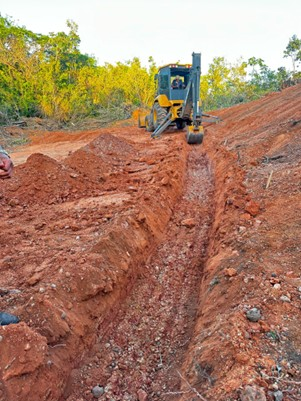
\includegraphics[width=0.8\linewidth,height=\textheight,keepaspectratio]{capitulos/../img/talude_campo.jpg}

}

\caption{\label{fig-talude}Talude em campo antes da intervenção ---
superfície exposta susceptível à erosão laminar e concentrada,
demandando reconfiguração geométrica e revegetação para estabilização.}

\end{figure}%

\subsection{Princípios}\label{princuxedpios}

O retaludamento vegetado baseia-se em quatro princípios complementares.
O primeiro é a redução do ângulo de inclinação do talude para valores
inferiores ao ângulo de repouso do material, o que aumenta o fator de
segurança por redução da componente de tensão cisalhante atuante. O
segundo é a criação de bermas intermediárias a cada 5--8 m de altura,
que funcionam como plataformas de captação de água e sedimentos,
interrompendo o comprimento de rampa e reduzindo a energia do escoamento
superficial. O terceiro é a revegetação das superfícies reconformadas
com espécies de raízes profundas e fasciculadas, que incrementam a
coesão do solo e reduzem a poropressão por evapotranspiração. O quarto é
a implantação de sistema de drenagem naturalizado (canaletas verdes,
conforme \textbf{?@sec-canaleta-verde}), que conduz o escoamento
interceptado pelas bermas sem gerar concentração erosiva.

\subsection{Dimensionamento}\label{dimensionamento-6}

A inclinação do talude retaludado deve atender ao fator de segurança
mínimo de 1,5 contra ruptura por cisalhamento, calculado pela análise de
estabilidade de taludes infinitos

\[
FS = \frac{\tau_f}{\tau_a} = \frac{c' + (\sigma - u) \tan \phi'}{(\gamma \cdot z \cdot \cos\beta) \cdot \sin\beta} \geq 1,5
\]

onde \(c'\) é a coesão efetiva do solo (kPa), \(\phi'\) é o ângulo de
atrito efetivo (°), \(\sigma\) é a tensão normal atuante na superfície
potencial de ruptura (kPa), \(u\) é a poropressão (kPa, dependente da
posição do lençol freático), \(\gamma\) é o peso específico do solo
(kN/m³), \(z\) é a profundidade da superfície de ruptura (m) e \(\beta\)
é o ângulo de inclinação do talude com a horizontal (°).

A contribuição da vegetação à estabilidade é quantificada pelo
incremento de coesão radicular (\(\Delta c_r\)), que se soma à coesão do
solo

\[
c'_{total} = c'_{solo} + \Delta c_r
\]

onde \(\Delta c_r\) é a coesão radicular adicional, calculável pelo
modelo de Wu-Waldron conforme detalhado em \textbf{?@sec-gabiao-vivo}.
Para gramíneas densas, \(\Delta c_r\) situa-se entre 2--5 kPa; para
arbustos com raízes profundas, entre 5--15 kPa; e para espécies arbóreas
com 3--5 anos, entre 10--25 kPa.

\section{Casos de Aplicação em Regiões
Tropicais}\label{casos-de-aplicauxe7uxe3o-em-regiuxf5es-tropicais}

\subsection{Semiárido brasileiro}\label{semiuxe1rido-brasileiro}

No semiárido, o desafio central reside na pluviosidade concentrada em
3--4 meses, com chuvas convectivas de alta intensidade sobre solos rasos
e vegetação de caatinga. A estratégia NBS para essas condições combina
paliçadas de madeira nas feições erosivas lineares
(\textbf{?@sec-palicadas}), bacias de captação para armazenamento
descentralizado de enxurradas (\textbf{?@sec-bacias-captacao}) e
revegetação com espécies nativas xerófitas adaptadas ao déficit hídrico
prolongado, complementada por Bio-SAP para retenção hídrica na zona
radicular (\textbf{?@sec-biopolimeros}). Essa abordagem integrada tem
demonstrado redução de escoamento superficial de 50--80\% e aumento
significativo de cobertura vegetal em parcelas experimentais.

\subsection{Encostas da Mata
Atlântica}\label{encostas-da-mata-atluxe2ntica}

Nas encostas da Mata Atlântica, a precipitação intensa (superior a 2.000
mm/ano), os solos profundos com mantos de intemperismo espessos e a
susceptibilidade a movimentos de massa demandam soluções de maior
robustez mecânica. A combinação de gabiões vivos na base das encostas
(\textbf{?@sec-gabiao-vivo}), paredes Krainer nas zonas de maior
solicitação (\textbf{?@sec-parede-krainer}) e revegetação com espécies
arbóreas pioneiras de crescimento rápido tem promovido a estabilização
de encostas com fator de segurança superior a 1,5 e regeneração
florestal progressiva, com cobertura de dossel superior a 70\% em 5
anos.

\subsection{Margens do rio São
Francisco}\label{margens-do-rio-suxe3o-francisco}

Nas margens do Baixo São Francisco, a erosão marginal acelerada
pós-barragem (resultante da alteração do regime hidrológico natural pela
operação de Xingó) em solos arenosos de baixa coesão constitui o
principal desafio geomorfológico. A associação de enrocamento vegetado
na linha d'água (\textbf{?@sec-enrocamento}), biotêxteis de taboa na
zona de variação de nível (\textbf{?@sec-biotexteis}) e geotêxteis
híbridos no talude superior (\textbf{?@sec-geotexteis}) reduziu a taxa
de recuo marginal em 70--90\%, conforme dados de monitoramento
topográfico por GNSS com levantamentos semestrais ao longo de 5 anos.

\begin{tcolorbox}[enhanced jigsaw, leftrule=.75mm, colframe=quarto-callout-note-color-frame, colback=white, bottomrule=.15mm, opacityback=0, colbacktitle=quarto-callout-note-color!10!white, breakable, bottomtitle=1mm, opacitybacktitle=0.6, title=\textcolor{quarto-callout-note-color}{\faInfo}\hspace{0.5em}{NBS e ODS}, titlerule=0mm, toprule=.15mm, toptitle=1mm, rightrule=.15mm, left=2mm, arc=.35mm, coltitle=black]

As Soluções Baseadas na Natureza contribuem diretamente para os
Objetivos de Desenvolvimento Sustentável 6 (Água limpa e saneamento), 11
(Cidades e comunidades sustentáveis), 13 (Ação contra a mudança global
do clima) e 15 (Vida terrestre), consolidando a bioengenharia de solos
como instrumento de política pública ambiental alinhado com compromissos
internacionais.

\end{tcolorbox}

\section{Adaptação às Mudanças
Climáticas}\label{adaptauxe7uxe3o-uxe0s-mudanuxe7as-climuxe1ticas}

\subsection{Projeções de Precipitação Extrema para Regiões
Tropicais}\label{projeuxe7uxf5es-de-precipitauxe7uxe3o-extrema-para-regiuxf5es-tropicais}

Os cenários de mudanças climáticas do IPCC (AR6, 2021) projetam, para as
regiões tropicais da América do Sul, um aumento na intensidade dos
eventos extremos de precipitação de 10--30\% até 2050 (cenário SSP2-4.5)
e de 20--50\% até 2100 (cenário SSP5-8.5), mesmo em regiões onde a
precipitação média anual tende a diminuir. Essa aparente contradição
(chuvas médias menores, porém eventos extremos mais intensos) resulta do
aquecimento atmosférico, que aumenta a capacidade de retenção de vapor
d'água em 7\% por grau Celsius de aquecimento (relação de
Clausius-Clapeyron), concentrando a precipitação em eventos menos
frequentes porém mais violentos.

Para a bioengenharia de solos, essa projeção tem implicações diretas no
dimensionamento. O fator de erosividade da chuva (\(R\) da RUSLE) pode
aumentar em 15--40\% nas próximas décadas, o que exige que as estruturas
de contenção e dissipação sejam dimensionadas com fatores de segurança
majorados. Em termos práticos, a chuva de projeto para dimensionamento
de paliçadas, bacias de captação e canaletas verdes deve adotar período
de retorno de 25--50 anos (em vez dos 10 anos usualmente empregados) e
incorporar um fator de majoração climática (\(F_{cc} = 1{,}2\) a
\(1{,}3\)) sobre a intensidade da chuva calculada a partir de séries
históricas, conforme recomendações da WMO (\emph{World Meteorological
Organization}) para projetos com horizonte de projeto superior a 30
anos.

\subsection{Resiliência Climática da
Bioengenharia}\label{resiliuxeancia-climuxe1tica-da-bioengenharia}

A bioengenharia de solos apresenta vantagens intrínsecas de resiliência
climática em relação à engenharia convencional, precisamente porque seus
componentes vivos respondem adaptativamente às mudanças ambientais. As
estruturas vegetativas se adaptam autonomamente (o aprofundamento
radicular em resposta ao déficit hídrico aumenta a ancoragem em cenários
de seca prolongada, enquanto o adensamento aéreo em resposta à maior
pluviosidade amplia a interceptação de chuva). A redundância funcional
proporcionada pela diversidade de espécies garante que, se uma espécie
for prejudicada pela alteração climática, outras ocupem seu nicho
funcional. A capacidade de autorreparação permite que a vegetação
rebrote e restabeleça a cobertura após danos por eventos extremos,
diferentemente de estruturas de concreto cuja ruptura é irreversível sem
intervenção humana. Além disso, a flexibilidade estrutural dos materiais
vivos e biodegradáveis absorve deformações e solicitações dinâmicas sem
ruptura frágil (diferentemente do concreto, que rompe subitamente quando
sua capacidade é excedida).

\subsection{Sequestro de Carbono}\label{sequestro-de-carbono}

A bioengenharia de solos contribui para a mitigação das mudanças
climáticas por meio do sequestro de carbono em dois compartimentos. A
biomassa aérea e radicular das espécies vegetais utilizadas nas
intervenções sequestra 2--8 tC/ha/ano nos primeiros 10 anos (com taxas
mais elevadas em espécies arbóreas de rápido crescimento como eucalipto
e gliricídia), estabilizando-se em 0,5--2,0 tC/ha/ano após a maturidade.
O carbono orgânico do solo (COS) aumenta pela decomposição de raízes
finas, serrapilheira e biotêxteis biodegradáveis, com incrementos de
0,3--1,5 tC/ha/ano ao longo dos primeiros 20 anos, particularmente em
solos tropicais com COS inicial depletado pela degradação.

A Tabela~\ref{tbl-carbono} sintetiza o potencial de sequestro de carbono
das principais técnicas de bioengenharia, permitindo a estimativa de
créditos de carbono para análise de viabilidade econômica.

\begin{longtable}[]{@{}
  >{\raggedright\arraybackslash}p{(\linewidth - 6\tabcolsep) * \real{0.1364}}
  >{\raggedright\arraybackslash}p{(\linewidth - 6\tabcolsep) * \real{0.3333}}
  >{\raggedright\arraybackslash}p{(\linewidth - 6\tabcolsep) * \real{0.1667}}
  >{\raggedright\arraybackslash}p{(\linewidth - 6\tabcolsep) * \real{0.3636}}@{}}
\caption{Potencial de sequestro de carbono das técnicas de bioengenharia
de solos.}\label{tbl-carbono}\tabularnewline
\toprule\noalign{}
\begin{minipage}[b]{\linewidth}\raggedright
Técnica
\end{minipage} & \begin{minipage}[b]{\linewidth}\raggedright
Sequestro (tC/ha/ano)
\end{minipage} & \begin{minipage}[b]{\linewidth}\raggedright
Horizonte
\end{minipage} & \begin{minipage}[b]{\linewidth}\raggedright
Compartimento dominante
\end{minipage} \\
\midrule\noalign{}
\endfirsthead
\toprule\noalign{}
\begin{minipage}[b]{\linewidth}\raggedright
Técnica
\end{minipage} & \begin{minipage}[b]{\linewidth}\raggedright
Sequestro (tC/ha/ano)
\end{minipage} & \begin{minipage}[b]{\linewidth}\raggedright
Horizonte
\end{minipage} & \begin{minipage}[b]{\linewidth}\raggedright
Compartimento dominante
\end{minipage} \\
\midrule\noalign{}
\endhead
\bottomrule\noalign{}
\endlastfoot
Revegetação com gramíneas & 1,0--3,0 & 5--10 anos & COS (raízes
finas) \\
Revegetação arbórea (espécies nativas) & 3,0--8,0 & 10--30 anos &
Biomassa aérea + COS \\
Enrocamento vegetado + mata ciliar & 2,0--6,0 & 5--20 anos & Biomassa +
sedimento retido \\
Biomantas + hidrossemeadura & 0,5--2,0 & 2--5 anos & COS (biodegradação
da manta) \\
Bio-SAP + geocompostos & 0,3--1,0 & 1--3 anos & COS (biodegradação do
polímero) \\
\end{longtable}

A monetização do carbono sequestrado pelos mercados voluntários de
créditos de carbono (R\$ 40--120/tC em 2025) pode representar receita
adicional de R\$ 200--600/ha/ano para projetos de bioengenharia com
revegetação arbórea, constituindo um mecanismo de financiamento
complementar que melhora a relação custo-benefício e favorece a
viabilidade econômica de intervenções em larga escala.

\section{Marco Regulatório e
Certificação}\label{marco-regulatuxf3rio-e-certificauxe7uxe3o}

\subsection{Normas Brasileiras
Aplicáveis}\label{normas-brasileiras-aplicuxe1veis}

O projeto e a execução de obras de bioengenharia de solos no Brasil
devem observar um conjunto de normas técnicas e regulamentos ambientais
cuja conformidade é condição indispensável para aprovação por órgãos
ambientais licenciadores e para financiamento por agências de fomento.
No âmbito da ABNT, aplicam-se a NBR 11682 (Estabilidade de encostas, que
define critérios de investigação geotécnica, análise de estabilidade e
plano de monitoramento), a NBR 16308 (Biomantas e biotêxteis para
controle de erosão, que classifica e especifica requisitos de desempenho
para produtos de fibras naturais), a NBR 10514 (Gabiões e colchões reno,
que regulamenta materiais, fabricação e montagem de cestas metálicas) e
a NBR 7229 (Ensaio de infiltração, fundamental para o dimensionamento de
bacias de captação e drenagem subsuperficial).

\subsection{Legislação Ambiental}\label{legislauxe7uxe3o-ambiental}

A legislação ambiental brasileira estabelece obrigações específicas que
condicionam o projeto de bioengenharia. O Código Florestal (Lei
12.651/2012) define as Áreas de Preservação Permanente (APP) onde
intervenções de revegetação e estabilização de encostas são
obrigatórias, exigindo o uso de espécies nativas nos projetos de
recomposição. A Política Nacional de Recursos Hídricos (Lei 9.433/1997)
fundamenta a gestão por bacia hidrográfica, que é o paradigma espacial
das intervenções de bioengenharia. A Política Nacional de Pagamento por
Serviços Ambientais (Lei 14.119/2021) cria mecanismos de remuneração por
atividades de conservação do solo e da água, incluindo o controle de
erosão por bioengenharia, o que viabiliza o financiamento de projetos
por propriedades rurais e municípios.

\subsection{Certificações
Internacionais}\label{certificauxe7uxf5es-internacionais}

No âmbito internacional, as normas ISO 14001 (Sistemas de gestão
ambiental) e ISO 14040/14044 (Avaliação do ciclo de vida, ACV) fornecem
os frameworks para avaliar a pegada ambiental de materiais e técnicas de
bioengenharia, subsidiando a comparação objetiva com soluções
convencionais. A norma europeia EN 13383 (Armourstone, especificação de
pedras para enrocamento) é referência para dimensionamento de
enrocamento vegetado (ver \textbf{?@sec-enrocamento}), enquanto a ASTM
D6460 (Standard Practice for Determination of Rolled Erosion Control
Product Performance) estabelece protocolos de ensaio para biomantas e
geotêxteis.

\begin{tcolorbox}[enhanced jigsaw, leftrule=.75mm, colframe=quarto-callout-tip-color-frame, colback=white, bottomrule=.15mm, opacityback=0, colbacktitle=quarto-callout-tip-color!10!white, breakable, bottomtitle=1mm, opacitybacktitle=0.6, title=\textcolor{quarto-callout-tip-color}{\faLightbulb}\hspace{0.5em}{Incentivos financeiros}, titlerule=0mm, toprule=.15mm, toptitle=1mm, rightrule=.15mm, left=2mm, arc=.35mm, coltitle=black]

No Brasil, programas como o Programa de Conservação de Estradas Rurais
(DER-SP), o Programa Produtor de Água (ANA) e o Programa de Recuperação
de Áreas Degradadas (PRAD) oferecem financiamento e assistência técnica
para implantação de técnicas de bioengenharia, constituindo
oportunidades concretas para viabilizar projetos em escala municipal e
de bacia hidrográfica.

\end{tcolorbox}

\chapter{Objetivo}\label{objetivo}

\# Projeto Integrador \{\#sec-projeto-integrador\}

Este capítulo sintetiza os conhecimentos apresentados ao longo do livro
em um projeto integrador de bioengenharia de solos, demonstrando como
combinar múltiplas técnicas para resolver um problema real de degradação
em região tropical. O objetivo não é apresentar uma receita fixa, mas um
método de trabalho que permita ao projetista diagnosticar a situação de
campo, selecionar as técnicas apropriadas, dimensionar as estruturas e
monitorar os resultados, adaptando o projeto às condições locais de
solo, clima, declividade e disponibilidade de materiais. A
Figura~\ref{fig-vocoroca} mostra uma voçoroca ativa em solo tropical,
feição erosiva de grande porte que exemplifica o tipo de desafio que
demanda projeto integrado de múltiplas técnicas.

\begin{figure}

\centering{

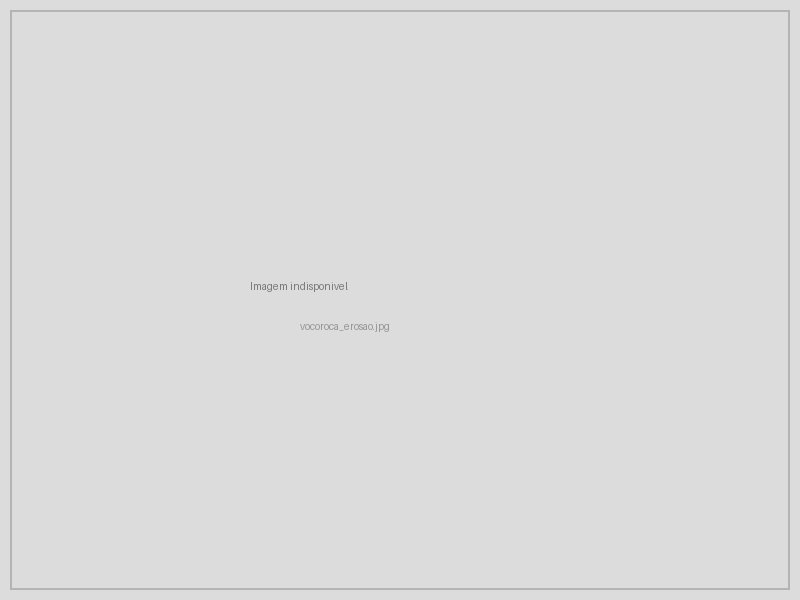
\includegraphics[width=0.85\linewidth,height=\textheight,keepaspectratio]{capitulos/../img/vocoroca_erosao.jpg}

}

\caption{\label{fig-vocoroca}Voçoroca ativa em solo tropical --- feição
erosiva de grande porte com paredes laterais instáveis, fundo com
escoamento concentrado e cabeceira em recuo ativo, demandando projeto
integrado de múltiplas técnicas de bioengenharia.}

\end{figure}%

\section{Metodologia de Projeto}\label{metodologia-de-projeto}

\subsection{Etapas do Projeto de
Bioengenharia}\label{etapas-do-projeto-de-bioengenharia}

O fluxograma a seguir apresenta as 7 etapas do projeto de bioengenharia
de solos, desde o diagnóstico de campo até a consolidação, incluindo o
ciclo de gestão adaptativa que retorna à seleção de técnicas caso as
metas de monitoramento não sejam atingidas.


\includegraphics[width=8in,height=3.5in]{capitulos/21-projeto-integrador_files/figure-latex/dot-figure-1.png}

\subsection{Etapa 1: Diagnóstico}\label{etapa-1-diagnuxf3stico}

O diagnóstico é a etapa mais crítica do projeto, pois a seleção
inadequada de técnicas resulta invariavelmente em ineficiência ou
fracasso da intervenção. O levantamento deve integrar seis componentes
fundamentais, cada um com método específico e produto cartográfico
associado, conforme a Tabela~\ref{tbl-diagnostico}.

\begin{longtable}[]{@{}
  >{\raggedright\arraybackslash}p{(\linewidth - 4\tabcolsep) * \real{0.4138}}
  >{\raggedright\arraybackslash}p{(\linewidth - 4\tabcolsep) * \real{0.2759}}
  >{\raggedright\arraybackslash}p{(\linewidth - 4\tabcolsep) * \real{0.3103}}@{}}
\caption{Componentes do diagnóstico integrado para projeto de
bioengenharia.}\label{tbl-diagnostico}\tabularnewline
\toprule\noalign{}
\begin{minipage}[b]{\linewidth}\raggedright
Componente
\end{minipage} & \begin{minipage}[b]{\linewidth}\raggedright
Método
\end{minipage} & \begin{minipage}[b]{\linewidth}\raggedright
Produto
\end{minipage} \\
\midrule\noalign{}
\endfirsthead
\toprule\noalign{}
\begin{minipage}[b]{\linewidth}\raggedright
Componente
\end{minipage} & \begin{minipage}[b]{\linewidth}\raggedright
Método
\end{minipage} & \begin{minipage}[b]{\linewidth}\raggedright
Produto
\end{minipage} \\
\midrule\noalign{}
\endhead
\bottomrule\noalign{}
\endlastfoot
Topografia & RPAS/drone + SfM (Structure from Motion) & MDE (Modelo
Digital de Elevação) com resolução ≤ 5 cm \\
Solos & Amostragem em campo + ensaios de laboratório & Mapa pedológico
com fator de erodibilidade K (RUSLE) \\
Clima & Estação meteorológica local ou interpolação & Série
pluviométrica com R de erosividade (RUSLE) \\
Cobertura & Classificação supervisionada de imagem orbital/drone & Mapa
de uso e cobertura com fator C (RUSLE) \\
Hidrologia & Modelagem de bacias (SIG) & Mapa de área contribuinte,
direções de fluxo e vazões \\
Vegetação & Inventário florístico de campo & Lista de espécies nativas
disponíveis para revegetação \\
\end{longtable}

A integração desses componentes em ambiente SIG permite a geração de
mapas de susceptibilidade à erosão e de priorização de intervenções,
fundamentais para a alocação eficiente de recursos em projetos de grande
escala espacial.

\subsection{Etapa 2: Classificação de
Feições}\label{etapa-2-classificauxe7uxe3o-de-feiuxe7uxf5es}

Utilizando a metodologia de classificação de feições erosivas
apresentada em \textbf{?@sec-classificacao-feicoes}, todas as feições
erosivas presentes na área de estudo devem ser mapeadas, medidas
(comprimento, largura, profundidade, área de seção transversal) e
classificadas segundo porte (sulco, ravina, voçoroca) e dinâmica (ativa,
estabilizada, reativada). A priorização das intervenções deve considerar
o risco associado a cada feição (proximidade de infraestrutura, taxa de
expansão, volume de sedimento exportado) e a relação custo-efetividade
do tratamento.

\subsection{Etapa 3: Seleção de
Técnicas}\label{etapa-3-seleuxe7uxe3o-de-tuxe9cnicas}

A seleção de técnicas segue uma matriz de decisão multicritério que
pondera sete variáveis, cada uma com peso proporcional à sua influência
no desempenho da intervenção, conforme a Tabela~\ref{tbl-selecao}.

\begin{longtable}[]{@{}
  >{\raggedright\arraybackslash}p{(\linewidth - 4\tabcolsep) * \real{0.2500}}
  >{\raggedright\arraybackslash}p{(\linewidth - 4\tabcolsep) * \real{0.1500}}
  >{\raggedright\arraybackslash}p{(\linewidth - 4\tabcolsep) * \real{0.6000}}@{}}
\caption{Critérios para seleção de técnicas de bioengenharia, com peso e
variáveis associadas.}\label{tbl-selecao}\tabularnewline
\toprule\noalign{}
\begin{minipage}[b]{\linewidth}\raggedright
Critério
\end{minipage} & \begin{minipage}[b]{\linewidth}\raggedright
Peso
\end{minipage} & \begin{minipage}[b]{\linewidth}\raggedright
Variáveis consideradas
\end{minipage} \\
\midrule\noalign{}
\endfirsthead
\toprule\noalign{}
\begin{minipage}[b]{\linewidth}\raggedright
Critério
\end{minipage} & \begin{minipage}[b]{\linewidth}\raggedright
Peso
\end{minipage} & \begin{minipage}[b]{\linewidth}\raggedright
Variáveis consideradas
\end{minipage} \\
\midrule\noalign{}
\endhead
\bottomrule\noalign{}
\endlastfoot
Tipo de feição & Alto & Classe EGC, profundidade, atividade
(ativa/estabilizada) \\
Solo & Alto & Textura, erodibilidade (K), coesão efetiva,
permeabilidade \\
Clima & Médio & Pluviosidade anual, intensidade de chuvas, déficit
hídrico \\
Inclinação & Alto & Ângulo do talude, comprimento de rampa, área
contribuinte \\
Acesso & Médio & Distância de vias, possibilidade de mecanização \\
Custo & Médio & Orçamento disponível, relação benefício/custo \\
Prazo & Baixo & Urgência da intervenção, cronograma de obras \\
\end{longtable}

A árvore de decisão a seguir operacionaliza a seleção de técnicas a
partir de perguntas-chave sobre a profundidade da feição, a presença de
água e as características do solo, direcionando o projetista para a
combinação de técnicas mais adequada.

\subsubsection{Árvore de Decisão}\label{uxe1rvore-de-decisuxe3o}

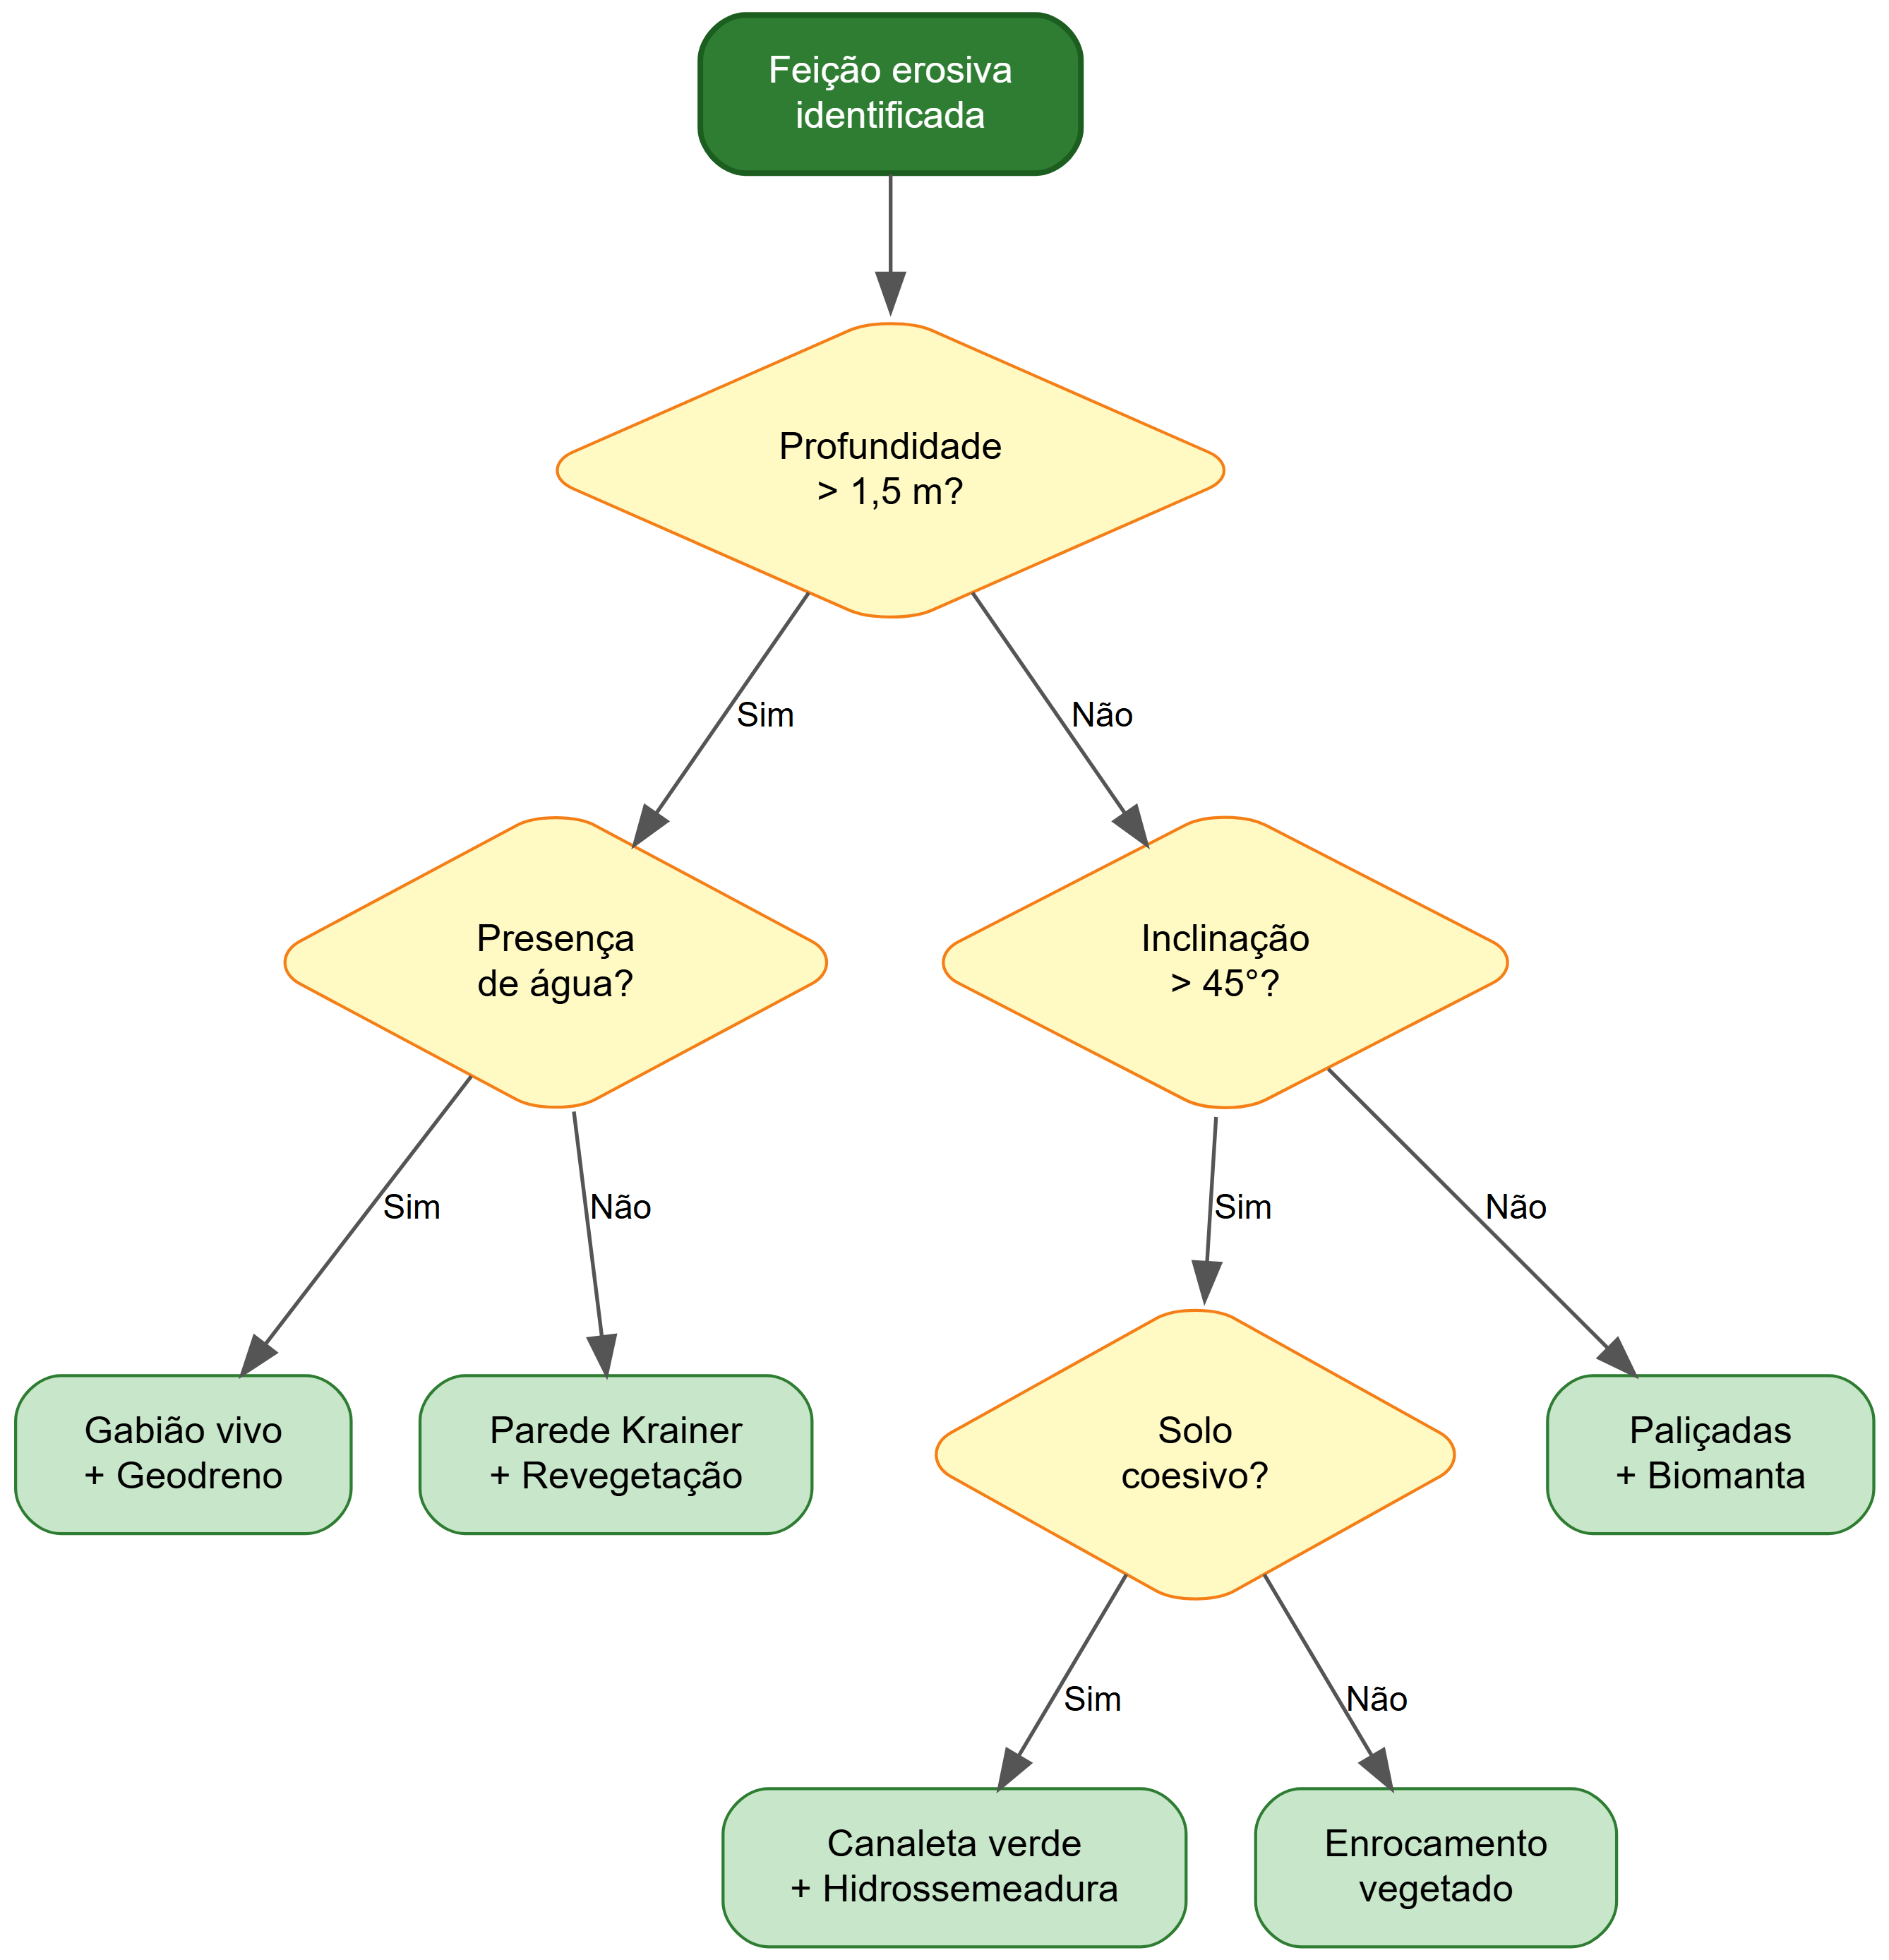
\includegraphics[width=8in,height=3.5in]{capitulos/21-projeto-integrador_files/figure-latex/dot-figure-3.png}

\subsection{Etapa 4: Dimensionamento}\label{etapa-4-dimensionamento}

Para cada técnica selecionada na etapa anterior, o dimensionamento deve
seguir os métodos específicos apresentados nos capítulos correspondentes
deste livro. O projetista deve consultar os capítulos de espaçamento e
altura de paliçadas (\textbf{?@sec-palicadas}), volume e arranjo de
bacias de captação (\textbf{?@sec-bacias-captacao}), taxa de aplicação
de hidrossemeadura (\textbf{?@sec-hidrossemeadura}), grampeamento e
sobreposição de biomantas (\textbf{?@sec-biomantas}), verificação de
estabilidade de gabiões vivos (\textbf{?@sec-gabiao-vivo}), geometria e
seleção de madeiras de paredes Krainer (\textbf{?@sec-parede-krainer}),
dimensionamento hidráulico de canaletas verdes
(\textbf{?@sec-canaleta-verde}) e critérios de filtração e resistência
de geotêxteis (\textbf{?@sec-geotexteis}). É fundamental que o
dimensionamento de cada elemento considere a interação com os demais,
pois as técnicas funcionam em sinergia (por exemplo, paliçadas a
montante reduzem a vazão de projeto das canaletas a jusante, e biomantas
reduzem a erosão que colmataria bacias de captação).

\subsection{Etapa 5: Projeto Executivo}\label{etapa-5-projeto-executivo}

O projeto executivo é o documento técnico que viabiliza a implantação em
campo e deve conter seis componentes obrigatórios. O memorial descritivo
apresenta as justificativas técnicas para cada decisão de projeto,
incluindo os resultados do diagnóstico, a classificação das feições e os
critérios de seleção de técnicas. As plantas de locação incluem a planta
geral (escala 1:500 a 1:2.000), seções transversais típicas (escala 1:50
a 1:100) e detalhes construtivos (escala 1:10 a 1:20) para cada tipo de
estrutura. As especificações técnicas definem os materiais (tipo de
madeira, granulometria do enrocamento, espécie e gramatura do geotêxtil,
composição da pasta de hidrossemeadura), as espécies vegetais (com
justificativa ecofisiológica) e as normas aplicáveis (ABNT, ASTM). O
cronograma de implantação define a sequência de fases, obrigatoriamente
iniciando pelas estruturas de drenagem e contenção antes da revegetação.
O orçamento detalha custos unitários e totais para cada item. O plano de
monitoramento define indicadores, métodos, frequência e metas
quantitativas para cada fase do projeto.

\subsection{Etapa 6: Implantação}\label{etapa-6-implantauxe7uxe3o}

A sequência de implantação é crítica para o sucesso do projeto, pois a
instalação de vegetação antes das estruturas de contenção e drenagem
expõe as mudas à energia erosiva não controlada. O diagrama de Gantt a
seguir apresenta o cronograma típico de implantação, com a sequência
preparo → estruturas → revegetação → monitoramento.

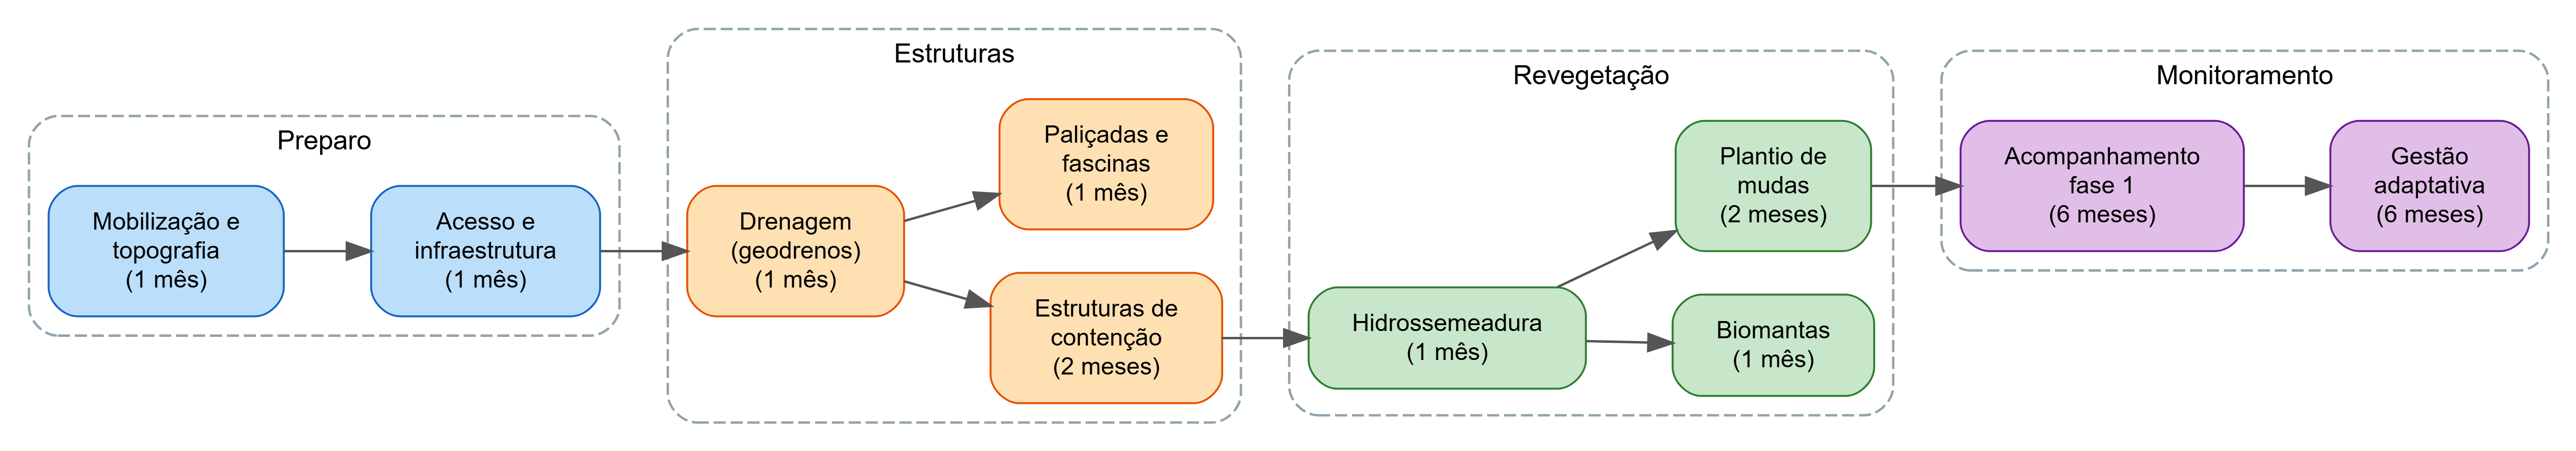
\includegraphics[width=8in,height=3.5in]{capitulos/21-projeto-integrador_files/figure-latex/dot-figure-2.png}

\begin{tcolorbox}[enhanced jigsaw, leftrule=.75mm, colframe=quarto-callout-warning-color-frame, colback=white, bottomrule=.15mm, opacityback=0, colbacktitle=quarto-callout-warning-color!10!white, breakable, bottomtitle=1mm, opacitybacktitle=0.6, title=\textcolor{quarto-callout-warning-color}{\faExclamationTriangle}\hspace{0.5em}{Período de implantação}, titlerule=0mm, toprule=.15mm, toptitle=1mm, rightrule=.15mm, left=2mm, arc=.35mm, coltitle=black]

A implantação da fase de revegetação deve coincidir com o início da
estação chuvosa para maximizar a taxa de estabelecimento da vegetação e
a sobrevivência de mudas. Em regiões semiáridas com período chuvoso
curto, irrigação suplementar pode ser necessária nos primeiros 60 dias
após o plantio, período em que as raízes ainda não atingiram
profundidade suficiente para acessar reservas hídricas do solo. O uso de
Bio-SAP (\textbf{?@sec-biopolimeros}) no substrato de plantio pode
reduzir a demanda de irrigação em 50--70\%.

\end{tcolorbox}

\subsection{Etapa 7: Monitoramento}\label{etapa-7-monitoramento}

O monitoramento é obrigatório em projetos de NBS (ver
\textbf{?@sec-nbs}), pois são sistemas vivos cuja resposta depende de
variáveis climáticas e biológicas não inteiramente controláveis. A
Tabela~\ref{tbl-monitoramento} define os indicadores mínimos, os métodos
de medição, a frequência recomendada e as metas quantitativas para cada
fase do projeto.

\begin{longtable}[]{@{}
  >{\raggedright\arraybackslash}p{(\linewidth - 6\tabcolsep) * \real{0.2973}}
  >{\raggedright\arraybackslash}p{(\linewidth - 6\tabcolsep) * \real{0.2162}}
  >{\raggedright\arraybackslash}p{(\linewidth - 6\tabcolsep) * \real{0.3243}}
  >{\raggedright\arraybackslash}p{(\linewidth - 6\tabcolsep) * \real{0.1622}}@{}}
\caption{Plano de monitoramento do projeto integrador, com indicadores,
métodos, frequência e metas.}\label{tbl-monitoramento}\tabularnewline
\toprule\noalign{}
\begin{minipage}[b]{\linewidth}\raggedright
Indicador
\end{minipage} & \begin{minipage}[b]{\linewidth}\raggedright
Método
\end{minipage} & \begin{minipage}[b]{\linewidth}\raggedright
Frequência
\end{minipage} & \begin{minipage}[b]{\linewidth}\raggedright
Meta
\end{minipage} \\
\midrule\noalign{}
\endfirsthead
\toprule\noalign{}
\begin{minipage}[b]{\linewidth}\raggedright
Indicador
\end{minipage} & \begin{minipage}[b]{\linewidth}\raggedright
Método
\end{minipage} & \begin{minipage}[b]{\linewidth}\raggedright
Frequência
\end{minipage} & \begin{minipage}[b]{\linewidth}\raggedright
Meta
\end{minipage} \\
\midrule\noalign{}
\endhead
\bottomrule\noalign{}
\endlastfoot
Cobertura vegetal (\%) & Fotografia aérea por RPAS/drone & Mensal (ano
1), trimestral (anos 2--3) & \textgreater{} 80\% em 12 meses \\
Taxa de sobrevivência (\%) & Contagem em parcelas permanentes &
Trimestral & \textgreater{} 70\% \\
Erosão (t/ha/ano) & Pinos de erosão + parcelas Wischmeier & Semestral &
\textless{} tolerância do solo local \\
Estabilidade do talude (FS) & Piezômetros + inclinômetros & Mensal
(estação chuvosa) & FS ≥ 1,5 \\
Qualidade da água & Análise de turbidez e sedimentos em suspensão &
Mensal & Turbidez \textless{} 100 NTU \\
\end{longtable}

\begin{figure}

\centering{

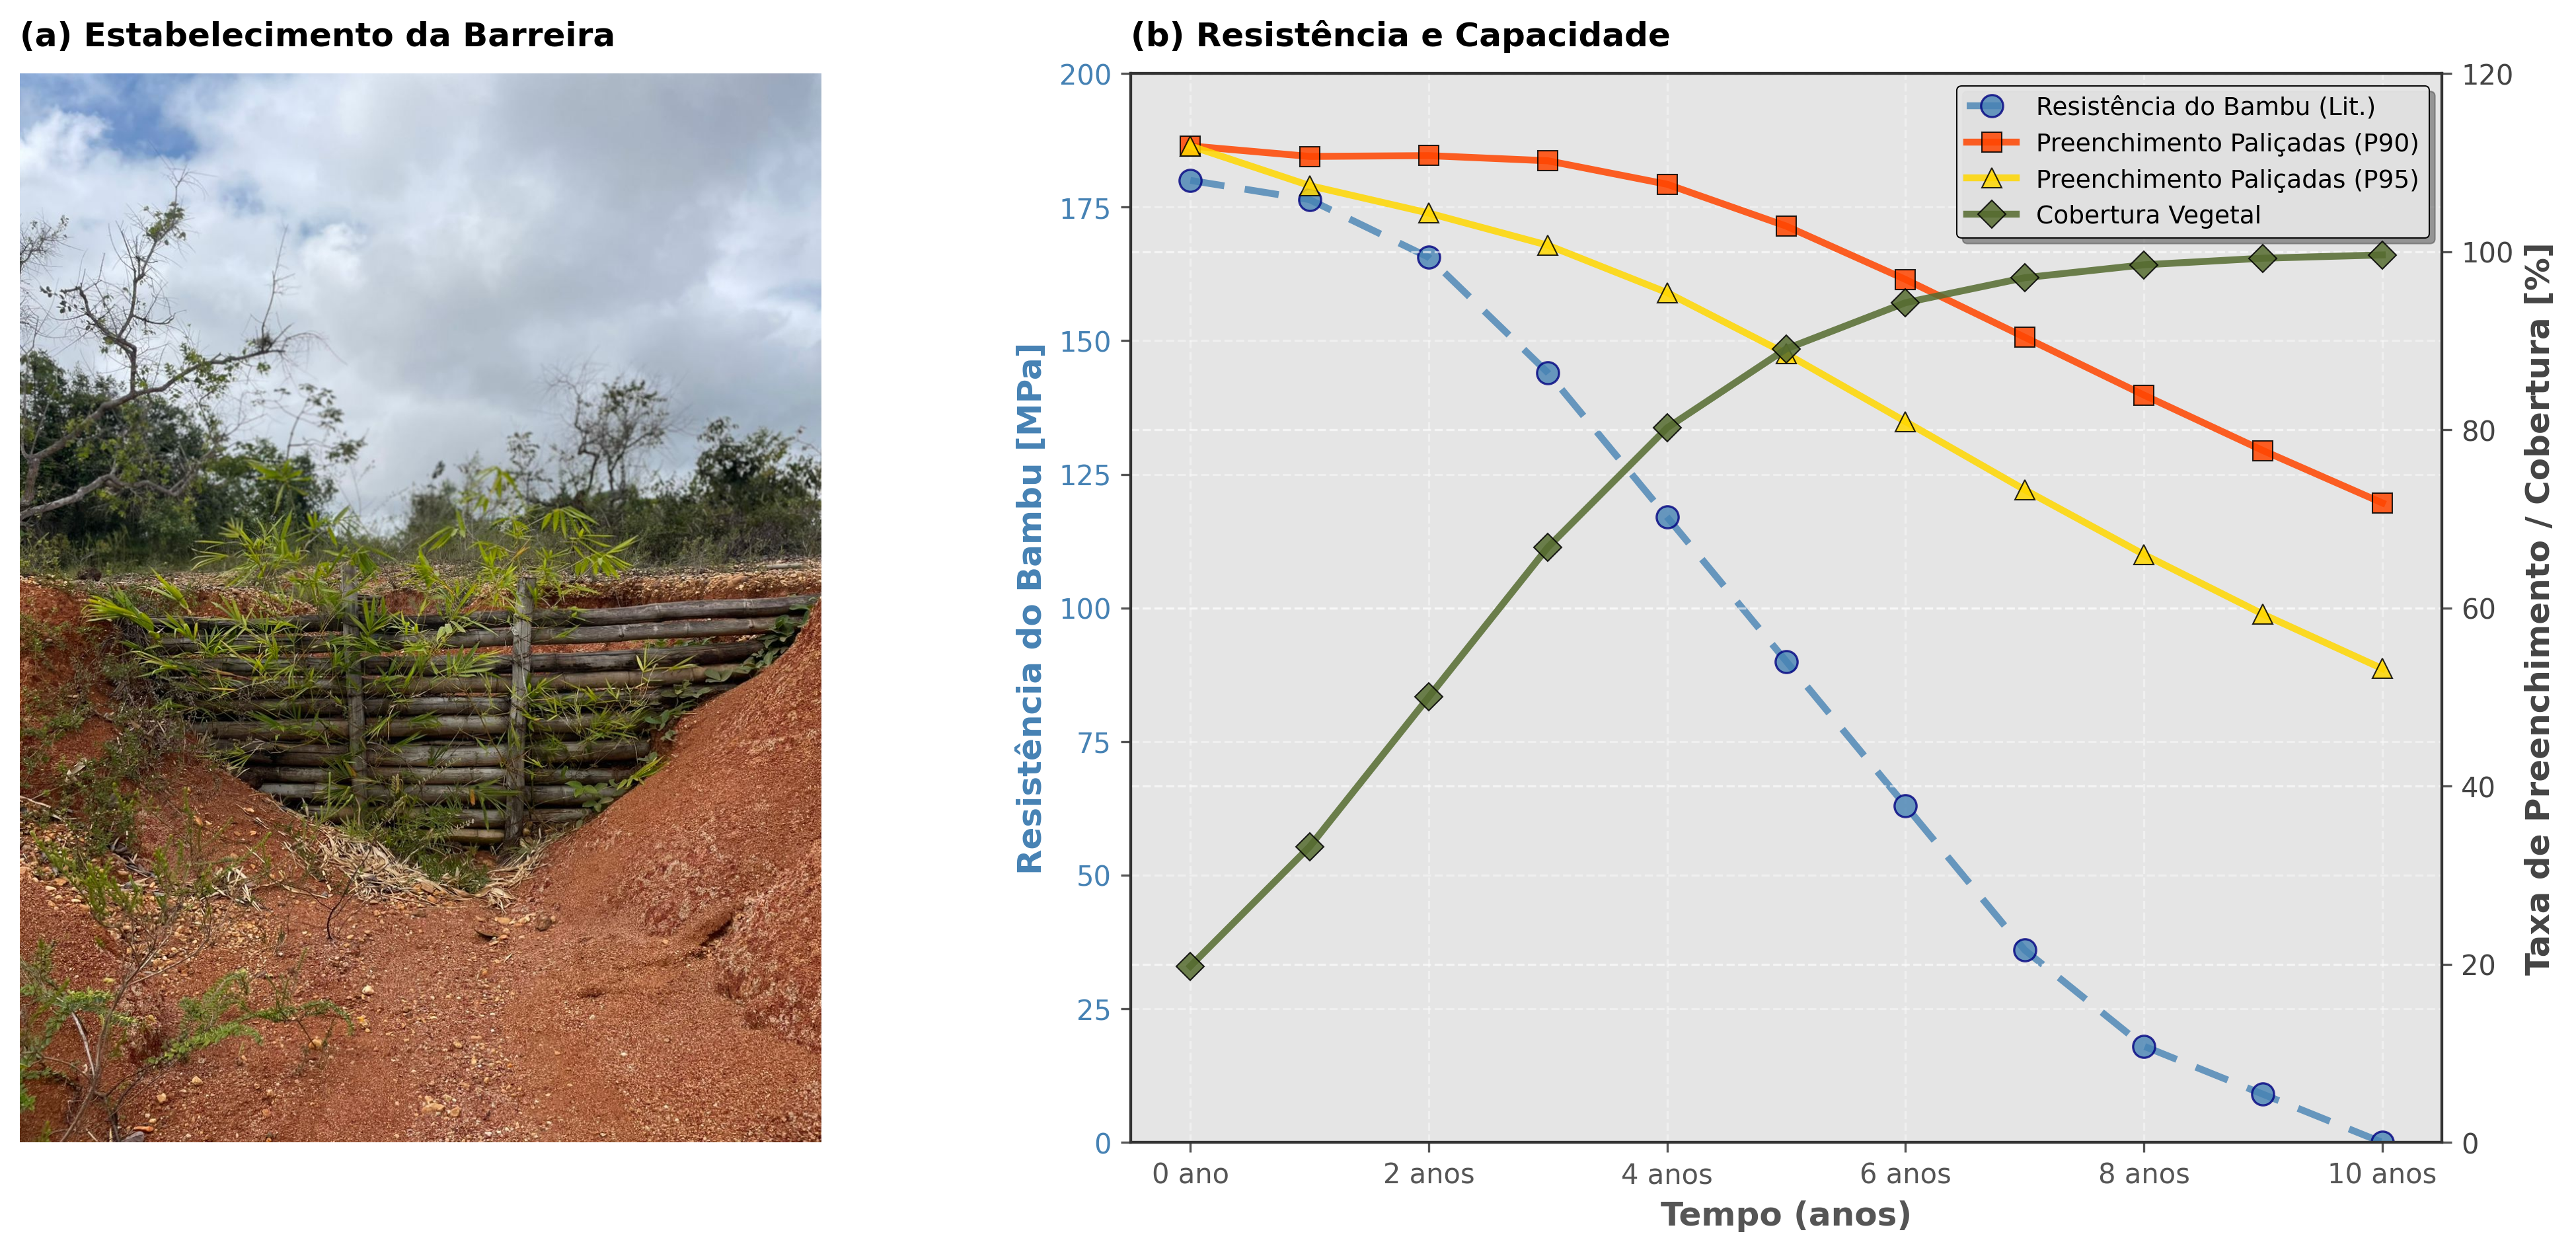
\includegraphics[width=0.9\linewidth,height=\textheight,keepaspectratio]{capitulos/../img/painel_integrado.png}

}

\caption{\label{fig-painel-integrado}Painel integrado de monitoramento
--- \emph{dashboard} que consolida indicadores de cobertura vegetal,
erosão, estabilidade de taludes e qualidade da água em uma interface
única de tomada de decisão.}

\end{figure}%

\section{Ferramentas Computacionais para
Modelagem}\label{ferramentas-computacionais-para-modelagem}

O projeto integrador de bioengenharia pode ser significativamente
potencializado pelo uso de ferramentas computacionais que automatizam
cálculos repetitivos, simulam cenários de intervenção e integram dados
espaciais de múltiplas fontes. As três categorias de ferramentas
apresentadas a seguir cobrem as necessidades computacionais mais
frequentes em projetos de bioengenharia.

\subsection{Modelagem Hidrológica
(SIG)}\label{modelagem-hidroluxf3gica-sig}

Os Sistemas de Informação Geográfica (SIG) são a plataforma central de
integração de dados espaciais em projetos de bioengenharia. A aplicação
da RUSLE em ambiente SIG permite calcular a perda de solo pixel a pixel
em toda a bacia contribuinte, identificando espacialmente os
\emph{hotspots} erosivos que devem ser priorizados. O QGIS (software
livre) com os plugins SAGA e GRASS oferece funcionalidades para
derivação automática de bacias hidrográficas a partir de MDE (Modelo
Digital de Elevação), cálculo dos fatores \(LS\), \(C\) e \(P\) da RUSLE
a partir de dados raster, modelagem de escoamento superficial pelo
método SCS-CN para estimativa de vazões de projeto e análise
multicritério para priorização de intervenções por sobreposição
ponderada de camadas temáticas.

\subsection{Estabilidade de Taludes}\label{estabilidade-de-taludes}

A análise de estabilidade de taludes é obrigatória para o
dimensionamento de gabiões vivos (ver \textbf{?@sec-gabiao-vivo}),
paredes Krainer (ver \textbf{?@sec-parede-krainer}) e retaludamento (ver
\textbf{?@sec-nbs}). Para análises em duas dimensões, os métodos de
equilíbrio-limite (Bishop simplificado, Janbu, Spencer) podem ser
executados com softwares como GeoStudio SLOPE/W, Slide2 (Rocscience) ou
GEOSLOPE, que calculam automaticamente o fator de segurança mínimo
(\(FS\)) por busca da superfície de ruptura crítica. A incorporação do
efeito da vegetação ao modelo requer a adição do termo de coesão
radicular (\(c_r\)) à coesão do solo na faixa de profundidade radicular
(0--2 m para gramíneas, 0--5 m para espécies arbóreas), além da
aplicação de uma sobrecarga correspondente ao peso da vegetação
(0,5--2,0 kPa para gramíneas, 2--5 kPa para arbustos e 5--15 kPa para
árvores).

A lógica do cálculo de estabilidade pode ser implementada em linguagem
Python para análises paramétricas rápidas. A equação do talude infinito
(adequada para rupturas superficiais em encostas com espessura de solo
homogênea) pode ser expressa como

\[
FS = \frac{c' + c_r + (\gamma \cdot z \cdot \cos^2\beta - u) \cdot \tan\phi'}{\gamma \cdot z \cdot \sin\beta \cdot \cos\beta}
\]

onde a inclusão explícita de \(c_r\) (coesão radicular) permite
quantificar o ganho de estabilidade proporcionado pela vegetação para
diferentes combinações de profundidade de raiz, densidade radicular e
espécie vegetal. Variando sistematicamente os parâmetros \(c_r\) (0 a 25
kPa), \(u\) (0 a \(\gamma_w \cdot z\)) e \(\beta\) (15° a 60°), o
projetista pode gerar abácos de decisão que indicam, para cada condição
de campo, se a revegetação sozinha é suficiente (\(FS \geq 1{,}5\)) ou
se estruturas complementares (gabiões, Krainer) são necessárias.

\subsection{Modelagem de Erosão e
Deposição}\label{modelagem-de-erosuxe3o-e-deposiuxe7uxe3o}

Para feições erosivas complexas (voçorocas com múltiplas cabeceiras,
contribuição de lençol freático, \emph{piping}), modelos de erosão
distribuídos como WEPP (\emph{Water Erosion Prediction Project}) e LISEM
(\emph{Limburg Soil Erosion Model}) oferecem simulação física dos
processos de desprendimento, transporte e deposição de sedimentos em
escala de evento ou contínua, incorporando a variabilidade espacial de
solo, cobertura e topografia. Esses modelos, embora mais complexos que a
RUSLE, permitem simular o efeito de intervenções pontuais (como
paliçadas ou bacias de captação) na redistribuição de sedimentos ao
longo da feição, subsidiando o posicionamento ótimo das estruturas.

A modelagem computacional não substitui o julgamento do engenheiro nem a
investigação de campo, mas acelera o processo de projeto, permite a
avaliação quantitativa de múltiplos cenários de intervenção antes da
implantação e fornece subsídios técnicos auditáveis para justificar
decisões de projeto perante órgãos licenciadores e financiadores.

\section{Estudo de Caso: Voçoroca em Latossolo no
Cerrado}\label{estudo-de-caso-vouxe7oroca-em-latossolo-no-cerrado}

\subsection{Cenário}\label{cenuxe1rio}

O estudo de caso exemplifica a aplicação do método de projeto a uma
situação real na Bacia do Rio São Francisco (MG). O local apresenta
Latossolo Vermelho-Amarelo de textura argilosa, sob clima Aw (Köppen)
com precipitação média anual de 1.200 mm concentrada em 6 meses (outubro
a março). A feição erosiva consiste em uma voçoroca ativa de 120 m de
comprimento, 15 m de largura média e 8 m de profundidade máxima, com
área de bacia contribuinte de 12 ha e uso anterior de pastagem degradada
com cobertura vegetal inferior a 40\%.

\subsection{Diagnóstico}\label{diagnuxf3stico}

A aplicação do modelo RUSLE (Revised Universal Soil Loss Equation) ao
cenário permite estimar a perda de solo antes da intervenção. A
erodibilidade do solo (\(K\)) foi determinada em 0,028 t·h/(MJ·mm) por
nomograma de Wischmeier a partir dos resultados de análise
granulométrica e teor de matéria orgânica. A erosividade da chuva
(\(R\)), calculada a partir de 30 anos de dados pluviométricos da
estação meteorológica mais próxima, resultou em 7.500 MJ·mm/(ha·h·ano).
O fator topográfico (\(LS\)), derivado do MDE com resolução de 5 cm
obtido por aerofotogrametria com drone, foi de 4,2 para o trecho mais
crítico. O fator de cobertura (\(C\)), determinado por classificação
supervisionada de imagem orbital, resultou em 0,35 (característico de
pastagem degradada com solo parcialmente exposto). O fator de práticas
conservacionistas (\(P\)) foi de 1,0, indicando ausência total de
práticas de conservação.

A perda de solo estimada pela RUSLE resulta em

\[
A = R \cdot K \cdot LS \cdot C \cdot P = 7.500 \times 0{,}028 \times 4{,}2 \times 0{,}35 \times 1{,}0 = 308{,}7 \text{ t/ha/ano}
\]

valor que excede em mais de 30 vezes a tolerância de perda de solo para
Latossolos no Cerrado (tipicamente 9--12 t/ha/ano), confirmando a
necessidade urgente de intervenção.

\subsection{Projeto}\label{projeto}

A Tabela~\ref{tbl-plano-intervencao} apresenta o plano de intervenção
por zona da voçoroca, onde cada zona recebe a combinação de técnicas
mais adequada à sua função hidrossedimentológica. A cabeceira,
responsável pelo recuo ativo, recebe paliçadas e bacias de captação para
interceptar o escoamento concentrado. As paredes laterais, sujeitas a
instabilidade geotécnica, recebem gabiões vivos e geotêxtil de taboa. O
fundo, com escoamento concentrado, recebe drenos verdes e fascinas vivas
para dissipação de energia. A encosta contribuinte a montante, geradora
do escoamento erosivo, recebe hidrossemeadura e biomanta para proteção
imediata. O topo da encosta recebe revegetação arbórea para
interceptação de chuva e coesão radicular profunda.

\begin{longtable}[]{@{}
  >{\raggedright\arraybackslash}p{(\linewidth - 4\tabcolsep) * \real{0.1765}}
  >{\raggedright\arraybackslash}p{(\linewidth - 4\tabcolsep) * \real{0.3235}}
  >{\raggedright\arraybackslash}p{(\linewidth - 4\tabcolsep) * \real{0.5000}}@{}}
\caption{Plano de intervenção por zona da voçoroca, com técnicas e
dimensionamento
específicos.}\label{tbl-plano-intervencao}\tabularnewline
\toprule\noalign{}
\begin{minipage}[b]{\linewidth}\raggedright
Zona
\end{minipage} & \begin{minipage}[b]{\linewidth}\raggedright
Técnica(s)
\end{minipage} & \begin{minipage}[b]{\linewidth}\raggedright
Dimensionamento
\end{minipage} \\
\midrule\noalign{}
\endfirsthead
\toprule\noalign{}
\begin{minipage}[b]{\linewidth}\raggedright
Zona
\end{minipage} & \begin{minipage}[b]{\linewidth}\raggedright
Técnica(s)
\end{minipage} & \begin{minipage}[b]{\linewidth}\raggedright
Dimensionamento
\end{minipage} \\
\midrule\noalign{}
\endhead
\bottomrule\noalign{}
\endlastfoot
Cabeceira & Paliçadas permeáveis (3 linhas, \textbf{?@sec-palicadas}) +
bacias de captação (\textbf{?@sec-bacias-captacao}) & E = 5 m entre
linhas, H = 0,8 m; 25 bacias (V = 1,2 m³ cada) \\
Corpo (paredes laterais) & Gabiões vivos (\textbf{?@sec-gabiao-vivo}) +
geotêxtil de taboa (\textbf{?@sec-biotexteis}) & 3 camadas de gabiões,
H\_total = 3 m \\
Corpo (fundo) & Drenos verdes + fascinas vivas
(\textbf{?@sec-feixes-drenos}) & Dreno central + 6 laterais \\
Encosta contribuinte & Hidrossemeadura (\textbf{?@sec-hidrossemeadura})
+ biomanta C350 (\textbf{?@sec-biomantas}) & T\_a = 350 g/m², malha 25
mm \\
Topo & Revegetação arbórea (espécies do Cerrado) & Espaçamento 3 × 3 m =
1.111 mudas/ha \\
\end{longtable}

\subsection{Resultados Esperados
(Modelagem)}\label{resultados-esperados-modelagem}

A modelagem dos resultados esperados utiliza a mesma equação RUSLE com
os fatores \(C\) e \(P\) atualizados para refletir a progressão da
cobertura vegetal e a instalação das práticas conservacionistas.

No Ano 1, espera-se cobertura vegetal de 40--60\% (estabelecimento das
gramíneas por hidrossemeadura), com redução de erosão da ordem de 65\%
pela combinação das estruturas de contenção (paliçadas, gabiões) e da
proteção superficial (biomantas).

No Ano 3, a cobertura vegetal deve superar 80\% (consolidação da
hidrossemeadura e crescimento das mudas arbóreas), com fator de
segurança superior a 1,5 nos taludes estabilizados pela contribuição da
coesão radicular (\(\Delta c_r\)).

No Ano 5, com a vegetação arbórea estabelecida (\(C = 0{,}05\)) e todas
as práticas conservacionistas operacionais (\(P = 0{,}6\)), a perda de
solo estimada pela RUSLE resulta em

\[
A_{5} = 7.500 \times 0{,}028 \times 4{,}2 \times 0{,}05 \times 0{,}6 = 26{,}5 \text{ t/ha/ano}
\]

representando uma redução de 91,4\% em relação à condição
pré-intervenção (de 308,7 para 26,5 t/ha/ano), valor próximo à
tolerância de perda de solo para Latossolos no Cerrado.

\subsection{Orçamento Estimado}\label{oruxe7amento-estimado}

A Tabela~\ref{tbl-orcamento} apresenta o orçamento estimado para a
recuperação da voçoroca, com valores referenciais para o contexto do
Cerrado mineiro. Os custos unitários incluem material e mão de obra de
instalação.

\begin{longtable}[]{@{}lllll@{}}
\caption{Orçamento estimado para recuperação da voçoroca --- valores
referenciais incluindo material e mão de
obra.}\label{tbl-orcamento}\tabularnewline
\toprule\noalign{}
Item & Unidade & Quantidade & Custo Unit. (R\() | Total (R\)) & \\
\midrule\noalign{}
\endfirsthead
\toprule\noalign{}
Item & Unidade & Quantidade & Custo Unit. (R\() | Total (R\)) & \\
\midrule\noalign{}
\endhead
\bottomrule\noalign{}
\endlastfoot
Paliçadas de bambu & m & 150 & 45 & 6.750 \\
Bacias de captação & un & 25 & 120 & 3.000 \\
Gabião vivo (caixa 2×1×0,5 m) & un & 45 & 350 & 15.750 \\
Geotêxtil de taboa & m² & 600 & 28 & 16.800 \\
Hidrossemeadura & m² & 2.500 & 12 & 30.000 \\
Biomanta C350 & m² & 1.800 & 25 & 45.000 \\
Mudas arbóreas nativas & un & 500 & 8 & 4.000 \\
Mão de obra & h & 800 & 35 & 28.000 \\
Total & & & & 149.300 \\
\end{longtable}

\begin{tcolorbox}[enhanced jigsaw, leftrule=.75mm, colframe=quarto-callout-tip-color-frame, colback=white, bottomrule=.15mm, opacityback=0, colbacktitle=quarto-callout-tip-color!10!white, breakable, bottomtitle=1mm, opacitybacktitle=0.6, title=\textcolor{quarto-callout-tip-color}{\faLightbulb}\hspace{0.5em}{Custo-benefício}, titlerule=0mm, toprule=.15mm, toptitle=1mm, rightrule=.15mm, left=2mm, arc=.35mm, coltitle=black]

O custo estimado de R\$ 149.300 corresponde a aproximadamente R\$ 100/m
linear de voçoroca tratada, ou R\$ 12/m² de área estabilizada, valor
3--5× inferior ao de soluções convencionais com muro de concreto armado
para feições de porte equivalente (ver Tabela~\ref{tbl-custos-nbs} em
\textbf{?@sec-nbs}). Quando os co-benefícios de sequestro de carbono e
regulação hídrica são contabilizados, o retorno do investimento é
estimado em 5--8 anos.

\end{tcolorbox}

\section{Considerações Finais}\label{considerauxe7uxf5es-finais}

O projeto integrador demonstra que a combinação sinérgica de técnicas de
bioengenharia é significativamente mais eficaz do que o uso isolado de
qualquer uma delas, pois cada técnica atua em um compartimento
específico da feição erosiva (cabeceira, paredes laterais, fundo,
encosta contribuinte) e em uma escala temporal distinta (proteção
imediata por biomantas, contenção estrutural por gabiões, estabilização
radicular em 3--5 anos). O diagnóstico adequado do solo, do clima e das
feições erosivas é o fundamento insubstituível para a seleção correta de
intervenções, e a aplicação indiscriminada de técnicas sem diagnóstico é
a principal causa de insucesso em projetos de recuperação. O
monitoramento é obrigatório, não opcional, porque as NBS são sistemas
vivos cuja trajetória depende de variáveis climáticas, edáficas e
biológicas que exigem gestão adaptativa. O custo é competitivo,
especialmente quando os co-benefícios ambientais são contabilizados,
consolidando a bioengenharia de solos como uma solução baseada na
natureza que atende simultaneamente aos critérios de eficiência técnica,
viabilidade econômica e alinhamento com os Objetivos de Desenvolvimento
Sustentável.

\part{Parte V --- Monitoramento e Análise}

\chapter{Modelagem 3D de Sistemas Radiculares}\label{sec-modelagem-3d}

\section{Introdução à Fotogrametria Aplicada a
Raízes}\label{introduuxe7uxe3o-uxe0-fotogrametria-aplicada-a-rauxedzes}

A quantificação da contribuição mecânica das raízes na estabilidade de
taludes é um dos pilares da bioengenharia de solos. Conforme discutido
nos capítulos anteriores, os modelos de Wu
(\textbf{?@sec-solos-tropicais}) e Waldron dependem fundamentalmente de
dois parâmetros: a resistência à tração das raízes (\(\overline{t_R}\))
e a razão de área radicular (\emph{Root Area Ratio} --- RAR).
Tradicionalmente, o RAR é estimado por métodos bidimensionais ---
análise de perfis expostos em trincheiras ou contagem de raízes em
quadrículas ---, que subestimam o volume radicular em 20--40\% por não
capturarem a distribuição tridimensional das raízes.

A fotogrametria digital \emph{Structure from Motion} (SfM) representa
uma alternativa acessível e precisa para superação dessas limitações
(\textbf{westoby2012?}). A técnica permite reconstruir a geometria 3D
completa de objetos a partir de múltiplas fotografias tomadas de ângulos
diferentes, utilizando algoritmos de correspondência de pontos homólogos
e triangulação. A Figura~\ref{fig-fluxo-sfm} ilustra o fluxo de trabalho
completo, desde a captura fotográfica até a extração de parâmetros
geotécnicos.

\begin{figure}

\centering{

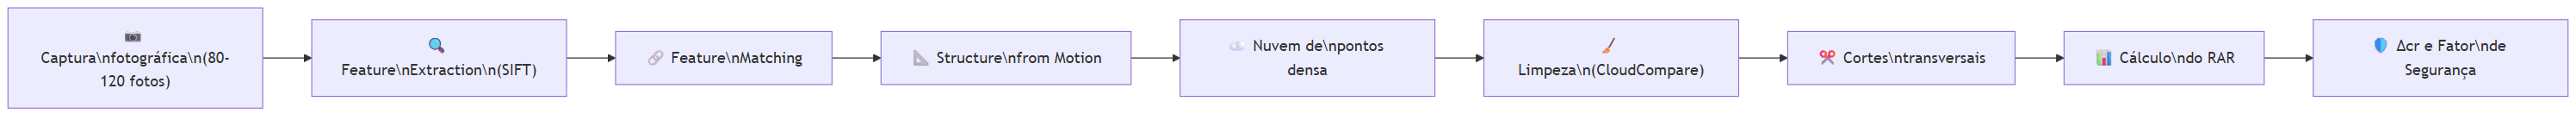
\includegraphics[width=27.38in,height=1.23in]{capitulos/22-modelagem-3d_files/figure-latex/mermaid-figure-1.png}

}

\caption{\label{fig-fluxo-sfm}Fluxograma do protocolo de fotogrametria
SfM para modelagem de sistemas radiculares: da captura fotográfica ao
cálculo do Fator de Segurança.}

\end{figure}%

As vantagens da SfM para aplicação em bioengenharia incluem baixo custo
(câmera de celular com ≥ 12 MP), portabilidade (uso direto em campo),
disponibilidade de software livre (Meshroom, CloudCompare) e resolução
submilimétrica (0,1--1,0 mm), suficiente para detectar raízes finas de
gramíneas como o vetiver.

\section{Preparação do Sítio
Experimental}\label{preparauxe7uxe3o-do-suxedtio-experimental}

\subsection{Critérios de Seleção}\label{crituxe9rios-de-seleuxe7uxe3o}

A seleção do sítio experimental deve considerar três critérios
principais: vegetação de vetiver ou outra espécie de interesse
estabelecida há pelo menos 6 meses (período mínimo para enraizamento
funcional), inclinação do talude entre 25° e 45° (faixa crítica para
erosão e instabilidade), e ausência de interferência antrópica recente.
As coordenadas geográficas e um croqui do local devem ser registrados.

\subsection{Abertura da Trincheira e Exposição das
Raízes}\label{abertura-da-trincheira-e-exposiuxe7uxe3o-das-rauxedzes}

A área de exposição é demarcada com estacas, formando um retângulo de no
mínimo 50 × 50 cm ao redor da touceira selecionada. A escavação deve ser
cuidadosa, mantendo as raízes íntegras, e aprofundada até a máxima
extensão visível --- tipicamente 60--100 cm para vetiver com mais de 12
meses. O jato de água a baixa pressão é utilizado para remover o solo
aderido sem romper raízes finas.

\begin{tcolorbox}[enhanced jigsaw, leftrule=.75mm, colframe=quarto-callout-tip-color-frame, colback=white, bottomrule=.15mm, opacityback=0, colbacktitle=quarto-callout-tip-color!10!white, breakable, bottomtitle=1mm, opacitybacktitle=0.6, title=\textcolor{quarto-callout-tip-color}{\faLightbulb}\hspace{0.5em}{Dica de Campo}, titlerule=0mm, toprule=.15mm, toptitle=1mm, rightrule=.15mm, left=2mm, arc=.35mm, coltitle=black]

Após a lavagem com jato d'água, aguarde 5--10 minutos para que as raízes
sequem superficialmente antes de fotografar. Raízes secas apresentam
melhor contraste com o solo, mas uma leve borrifada de água
imediatamente antes da captura melhora a textura visual nas fotos.

\end{tcolorbox}

\subsection{Montagem da Cena}\label{montagem-da-cena}

A preparação da cena para fotogrametria requer: (a) posicionamento de
escala métrica (trena graduada) em duas direções perpendiculares, (b)
distribuição de quatro alvos codificados ao redor da área de interesse,
em posições fixas e visíveis em todas as fotos, e (c) instalação de
painel de fundo neutro (lona cinza) atrás das raízes para reduzir ruído
no processamento.

\section{Aquisição Fotográfica}\label{aquisiuxe7uxe3o-fotogruxe1fica}

\subsection{Configuração da
Câmera}\label{configurauxe7uxe3o-da-cuxe2mera}

A câmera deve ser configurada em modo manual (M) ou prioridade de
abertura (Av), com ISO 100--400, abertura f/5.6 a f/8 (para máxima
profundidade de campo), velocidade ≥ 1/125 s, foco manual fixo e flash
desligado. A captura deve ser realizada sob iluminação difusa (céu
nublado) ou com sol baixo, evitando sombras projetadas sobre as raízes.

\subsection{Protocolo de Captura
Orbital}\label{protocolo-de-captura-orbital}

O protocolo de captura segue um padrão de órbitas concêntricas ao redor
do sistema radicular, conforme descrito na Tabela~\ref{tbl-orbitas}.

\begin{longtable}[]{@{}
  >{\centering\arraybackslash}p{(\linewidth - 8\tabcolsep) * \real{0.1194}}
  >{\centering\arraybackslash}p{(\linewidth - 8\tabcolsep) * \real{0.2239}}
  >{\centering\arraybackslash}p{(\linewidth - 8\tabcolsep) * \real{0.3134}}
  >{\centering\arraybackslash}p{(\linewidth - 8\tabcolsep) * \real{0.1940}}
  >{\raggedright\arraybackslash}p{(\linewidth - 8\tabcolsep) * \real{0.1493}}@{}}
\caption{Protocolo de captura fotográfica orbital para fotogrametria SfM
de raízes.}\label{tbl-orbitas}\tabularnewline
\toprule\noalign{}
\begin{minipage}[b]{\linewidth}\centering
Órbita
\end{minipage} & \begin{minipage}[b]{\linewidth}\centering
Distância (m)
\end{minipage} & \begin{minipage}[b]{\linewidth}\centering
Ângulo entre fotos
\end{minipage} & \begin{minipage}[b]{\linewidth}\centering
Nº de fotos
\end{minipage} & \begin{minipage}[b]{\linewidth}\raggedright
Objetivo
\end{minipage} \\
\midrule\noalign{}
\endfirsthead
\toprule\noalign{}
\begin{minipage}[b]{\linewidth}\centering
Órbita
\end{minipage} & \begin{minipage}[b]{\linewidth}\centering
Distância (m)
\end{minipage} & \begin{minipage}[b]{\linewidth}\centering
Ângulo entre fotos
\end{minipage} & \begin{minipage}[b]{\linewidth}\centering
Nº de fotos
\end{minipage} & \begin{minipage}[b]{\linewidth}\raggedright
Objetivo
\end{minipage} \\
\midrule\noalign{}
\endhead
\bottomrule\noalign{}
\endlastfoot
1 --- Contexto & 1,0--1,5 & 10--15° & 24--36 & Cobertura 360°, visão
geral \\
2 --- Média & 0,5--0,8 & 10° & 36 & Detalhamento intermediário \\
3 --- Detalhe & 0,3--0,5 & Livre & ≥ 20 & Close-ups de zonas densas \\
\end{longtable}

O total mínimo é de 80 fotos (recomendado: 100--120), com sobreposição ≥
70\% entre consecutivas. Cada ponto do objeto deve ser visível em pelo
menos 3 fotos de ângulos distintos, e a escala métrica deve aparecer em
≥ 50\% das imagens.

\subsection{Resolução Espacial
(GSD)}\label{resoluuxe7uxe3o-espacial-gsd}

A viabilidade da detecção de raízes finas depende da resolução espacial
das fotos, expressa pelo \emph{Ground Sampling Distance} (GSD):

\begin{equation}\phantomsection\label{eq-gsd-cap22}{GSD = \frac{d \times p}{f}}\end{equation}

onde \(d\) é a distância câmera-objeto (m), \(p\) é o tamanho do pixel
no sensor (mm) e \(f\) é a distância focal (mm). O critério adotado é
\(GSD \leq d_{min}/2\), onde \(d_{min}\) é o diâmetro da menor raiz a
detectar. Para raízes de vetiver (diâmetro ≈ 0,5 mm), o GSD deve ser ≤
0,25 mm/pixel --- facilmente alcançável com câmeras de 12 MP a 0,5 m de
distância.

\section{Processamento
Fotogramétrico}\label{processamento-fotogramuxe9trico}

\subsection{Pipeline no Meshroom}\label{pipeline-no-meshroom}

O processamento é realizado no Meshroom (AliceVision), software livre de
fotogrametria SfM. A pipeline padrão compreende 10 nós sequenciais
(Tabela~\ref{tbl-pipeline-meshroom}).

\begin{longtable}[]{@{}cll@{}}
\caption{Pipeline de processamento fotogramétrico no
Meshroom.}\label{tbl-pipeline-meshroom}\tabularnewline
\toprule\noalign{}
Passo & Nó & Configuração \\
\midrule\noalign{}
\endfirsthead
\toprule\noalign{}
Passo & Nó & Configuração \\
\midrule\noalign{}
\endhead
\bottomrule\noalign{}
\endlastfoot
1 & CameraInit & Auto-detecção \\
2 & FeatureExtraction & Descritor SIFT, qualidade Normal \\
3 & ImageMatching & VocabularyTree \\
4 & FeatureMatching & Sem limite \\
5 & StructureFromMotion & Padrão \\
6 & DepthMapEstimation & Resolução Normal \\
7 & DepthMapFiltering & Padrão \\
8 & Meshing & maxPoints: 5.000.000 \\
9 & MeshFiltering & Suavização fator 1 \\
10 & Texturing & 4096 × 4096 \\
\end{longtable}

\subsection{Verificação de
Qualidade}\label{verificauxe7uxe3o-de-qualidade}

Após o nó StructureFromMotion, o número de câmeras calibradas deve ser ≥
90\% das fotos importadas. Se inferior a 70\%, as fotos são
insuficientes e deve-se retornar ao campo. O tempo de processamento
varia de 30 minutos (80 fotos, GPU NVIDIA GTX 1060) a 8 horas (120
fotos, apenas CPU).

\begin{tcolorbox}[enhanced jigsaw, leftrule=.75mm, colframe=quarto-callout-warning-color-frame, colback=white, bottomrule=.15mm, opacityback=0, colbacktitle=quarto-callout-warning-color!10!white, breakable, bottomtitle=1mm, opacitybacktitle=0.6, title=\textcolor{quarto-callout-warning-color}{\faExclamationTriangle}\hspace{0.5em}{Requisito de Hardware}, titlerule=0mm, toprule=.15mm, toptitle=1mm, rightrule=.15mm, left=2mm, arc=.35mm, coltitle=black]

O Meshroom requer GPU NVIDIA com suporte CUDA para processamento em
tempo razoável. Se não disponível, alternativas como COLMAP (modo CPU)
ou Google Colab (GPU gratuita) podem ser utilizadas.

\end{tcolorbox}

\subsection{Exportação}\label{exportauxe7uxe3o}

Os produtos do processamento são a nuvem de pontos densa (formato
\texttt{.ply}, com cores RGB) e a malha texturizada (formato
\texttt{.obj} + \texttt{.mtl} + texturas \texttt{.png}).

\section{Análise no CloudCompare}\label{anuxe1lise-no-cloudcompare}

\subsection{Limpeza da Nuvem de
Pontos}\label{limpeza-da-nuvem-de-pontos}

O CloudCompare é o software utilizado para análise tridimensional. Após
importação do arquivo \texttt{.ply}, a limpeza compreende três etapas:
remoção manual de pontos do solo e fundo por segmentação poligonal (Edit
→ Segment), remoção estatística de outliers pelo \emph{Statistical
Outlier Removal} (SOR Filter, com 6 vizinhos e multiplicador 1,0--2,0),
e subamostragem por espaçamento mínimo de 0,5--1,0 mm quando necessário.

\subsection{Calibração de Escala}\label{calibrauxe7uxe3o-de-escala}

A escala é calibrada pela ferramenta \emph{Point Picking} (Tools → Point
Picking), medindo-se a distância entre dois pontos conhecidos na régua
graduada e aplicando-se o fator de correção \(k = d_{real}/d_{medida}\)
via Edit → Multiply/Scale nas três dimensões.

\subsection{Visualização por
Profundidade}\label{visualizauxe7uxe3o-por-profundidade}

A distribuição vertical das raízes é visualizada pela ferramenta
\emph{Height Ramp} (Edit → Colors → Height Ramp), com coloração no eixo
Z e paleta Blue-Green-Yellow-Red (azul = superficial, vermelho =
profundo). A Figura~\ref{fig-cloud-compare-exemplo} ilustra o resultado
típico.

\begin{figure}

\centering{

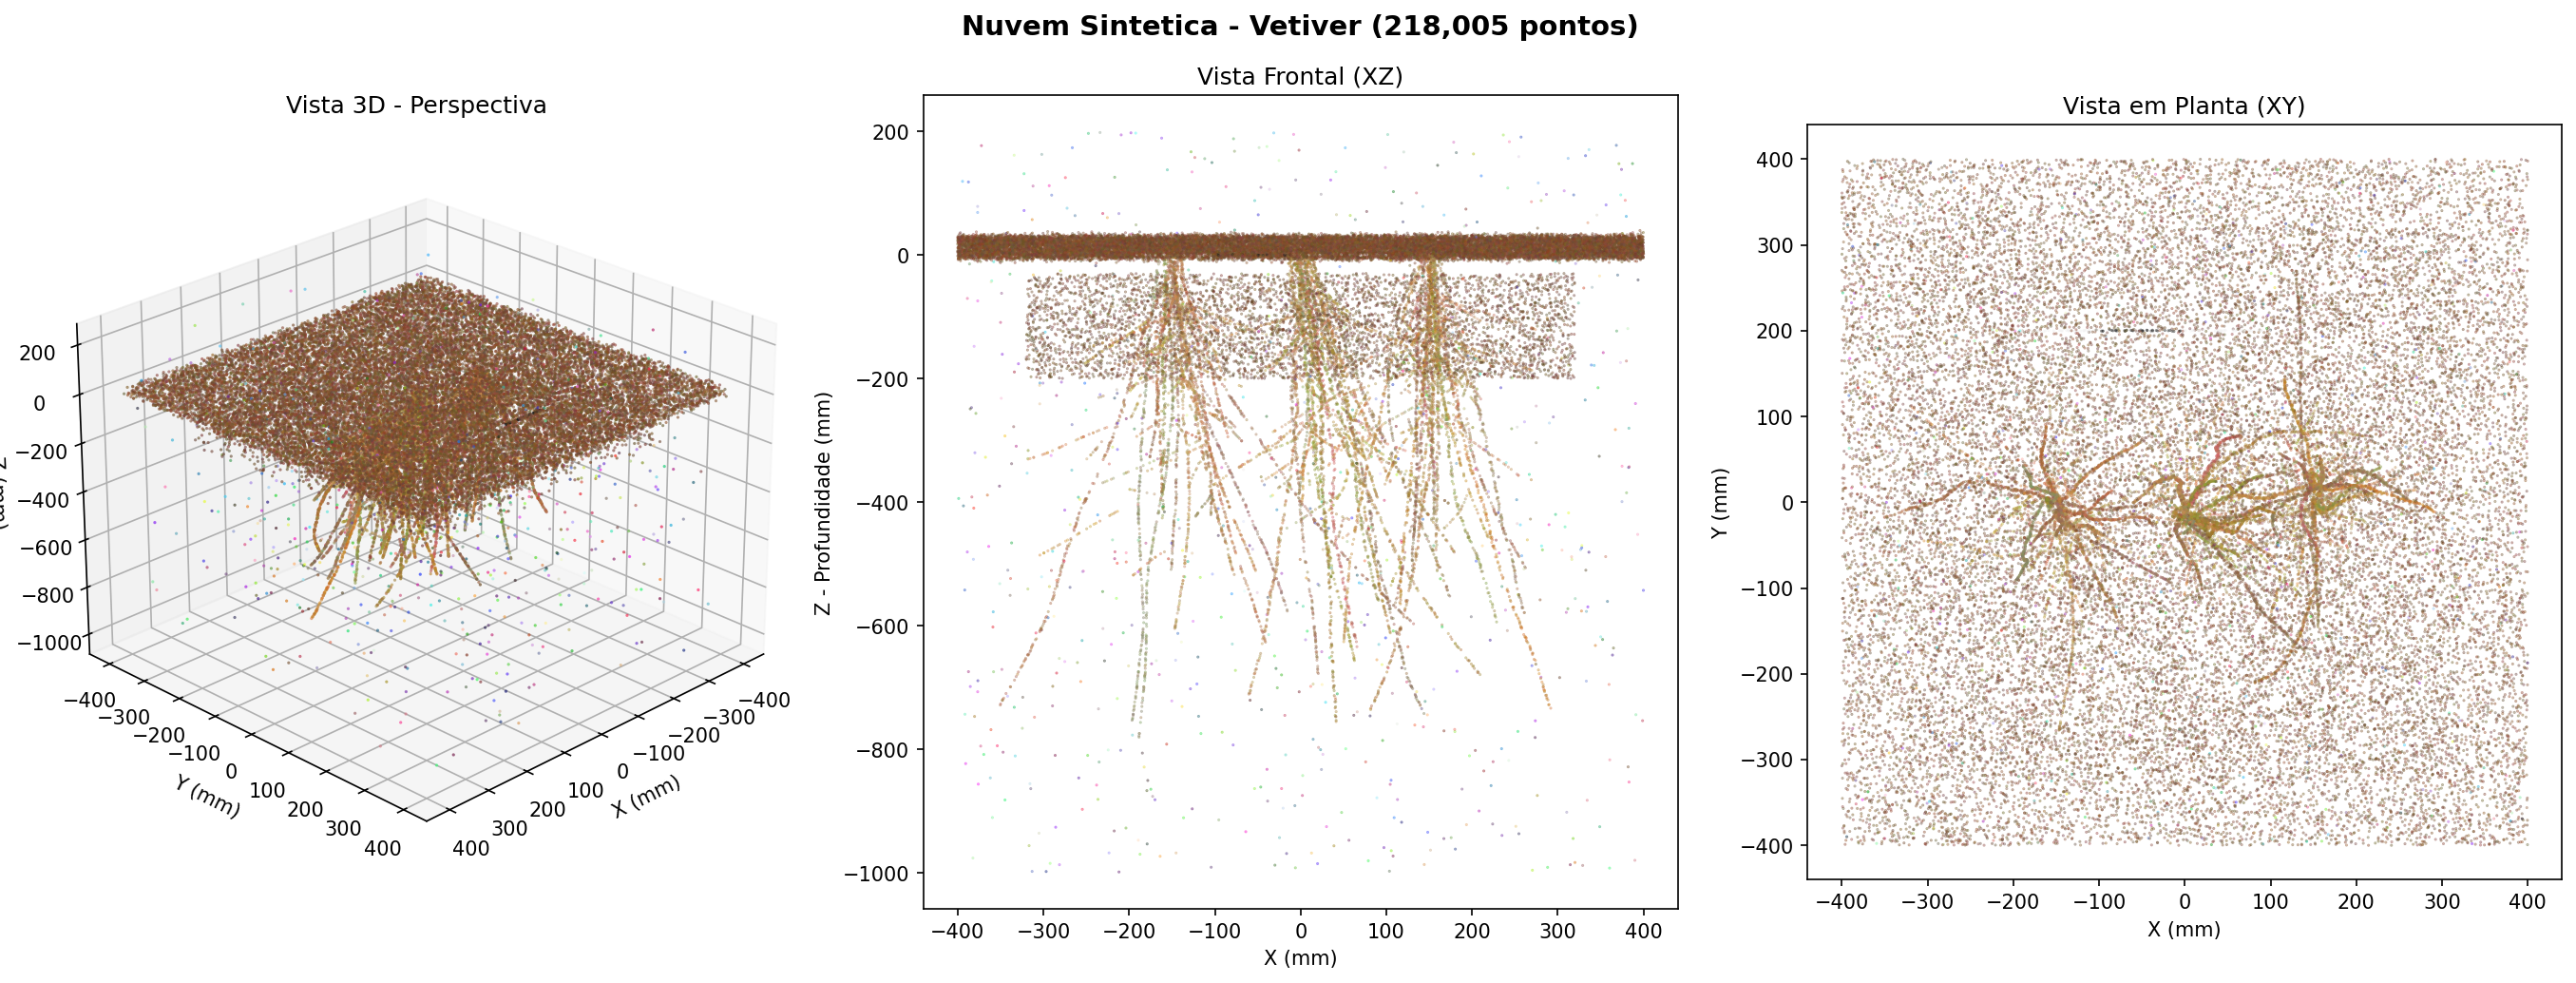
\includegraphics[width=0.8\linewidth,height=\textheight,keepaspectratio]{capitulos/../img/cloudcompare_raizes_vetiver.png}

}

\caption{\label{fig-cloud-compare-exemplo}Exemplo de nuvem de pontos de
sistema radicular de vetiver no CloudCompare, com coloração por
profundidade (Height Ramp): azul indica raízes superficiais e vermelho
indica raízes profundas.}

\end{figure}%

\section{Extração do RAR por Cortes
Transversais}\label{extrauxe7uxe3o-do-rar-por-cortes-transversais}

\subsection{Método de Fatiamento}\label{muxe9todo-de-fatiamento}

O RAR é o parâmetro principal extraído do modelo 3D. O procedimento
consiste em fatiar horizontalmente a nuvem de pontos em camadas de 10 cm
de espessura, utilizando a ferramenta \emph{Cross Section} (Tools →
Segmentation → Cross Section), com plano de corte XY.

Para cada fatia na profundidade \(z_i\), a nuvem é rasterizada no plano
XY (Tools → Projection → Rasterize, resolução de célula = 1 mm), e o RAR
é calculado como:

\begin{equation}\phantomsection\label{eq-rar-cap22}{RAR(z_i) = \frac{A_{raiz}}{A_{total}} = \frac{n_{raiz} \times A_{célula}}{n_{total} \times A_{célula}}}\end{equation}

onde \(n_{raiz}\) é o número de células ocupadas por raízes e
\(n_{total}\) é o total de células na área delimitadora.

\subsection{Resultados Típicos}\label{resultados-tuxedpicos}

A Tabela~\ref{tbl-rar-exemplo} apresenta valores típicos de RAR para
vetiver estabelecido há 18 meses em talude rodoviário com solo argiloso
tropical, obtidos por este protocolo.

\begin{longtable}[]{@{}
  >{\centering\arraybackslash}p{(\linewidth - 8\tabcolsep) * \real{0.1512}}
  >{\centering\arraybackslash}p{(\linewidth - 8\tabcolsep) * \real{0.2209}}
  >{\centering\arraybackslash}p{(\linewidth - 8\tabcolsep) * \real{0.2326}}
  >{\centering\arraybackslash}p{(\linewidth - 8\tabcolsep) * \real{0.1047}}
  >{\centering\arraybackslash}p{(\linewidth - 8\tabcolsep) * \real{0.2907}}@{}}
\caption{RAR e acréscimo de coesão por camada de profundidade para
vetiver com 18 meses.}\label{tbl-rar-exemplo}\tabularnewline
\toprule\noalign{}
\begin{minipage}[b]{\linewidth}\centering
Camada (cm)
\end{minipage} & \begin{minipage}[b]{\linewidth}\centering
\(A_{raiz}\) (cm²)
\end{minipage} & \begin{minipage}[b]{\linewidth}\centering
\(A_{total}\) (cm²)
\end{minipage} & \begin{minipage}[b]{\linewidth}\centering
RAR (\%)
\end{minipage} & \begin{minipage}[b]{\linewidth}\centering
\(\Delta c_r\) --- Wu (kPa)
\end{minipage} \\
\midrule\noalign{}
\endfirsthead
\toprule\noalign{}
\begin{minipage}[b]{\linewidth}\centering
Camada (cm)
\end{minipage} & \begin{minipage}[b]{\linewidth}\centering
\(A_{raiz}\) (cm²)
\end{minipage} & \begin{minipage}[b]{\linewidth}\centering
\(A_{total}\) (cm²)
\end{minipage} & \begin{minipage}[b]{\linewidth}\centering
RAR (\%)
\end{minipage} & \begin{minipage}[b]{\linewidth}\centering
\(\Delta c_r\) --- Wu (kPa)
\end{minipage} \\
\midrule\noalign{}
\endhead
\bottomrule\noalign{}
\endlastfoot
0--10 & 10,0 & 2500 & 0,40 & 7,2 \\
10--20 & 7,5 & 2500 & 0,30 & 5,4 \\
20--30 & 5,0 & 2500 & 0,20 & 3,6 \\
30--50 & 3,0 & 2500 & 0,12 & 2,2 \\
50--100 & 1,25 & 2500 & 0,05 & 0,9 \\
\end{longtable}

A distribuição é não linear, com concentração nas camadas superficiais:
80\% do efeito mecânico ocorre nos primeiros 50 cm.

\section{Estimativa do Acréscimo de
Coesão}\label{estimativa-do-acruxe9scimo-de-coesuxe3o}

\subsection{Modelo de Wu (1979)}\label{modelo-de-wu-1979}

Com os valores de RAR por camada, o acréscimo de coesão conferido pelas
raízes é estimado pelo modelo de Wu:

\begin{equation}\phantomsection\label{eq-wu-cap22}{\Delta c_r(z) = 1{,}2 \times \overline{t_R} \times RAR(z)}\end{equation}

onde \(\overline{t_R}\) é a resistência média à tração das raízes e o
fator 1,2 corrige a orientação aleatória. Para vetiver,
\(\overline{t_R}\) varia entre 40 e 180 MPa (média adotada: 75 MPa).

\begin{tcolorbox}[enhanced jigsaw, leftrule=.75mm, colframe=quarto-callout-important-color-frame, colback=white, bottomrule=.15mm, opacityback=0, colbacktitle=quarto-callout-important-color!10!white, breakable, bottomtitle=1mm, opacitybacktitle=0.6, title=\textcolor{quarto-callout-important-color}{\faExclamation}\hspace{0.5em}{Limitação do Modelo de Wu}, titlerule=0mm, toprule=.15mm, toptitle=1mm, rightrule=.15mm, left=2mm, arc=.35mm, coltitle=black]

O modelo de Wu assume que todas as raízes rompem simultaneamente, o que
na prática não ocorre. Estudos de (\textbf{pollen2005?}) demonstraram
superestimação de 50--100\% em relação a medições de campo. O modelo é
adequado para triagem preliminar, mas projetos executivos devem utilizar
o modelo de Waldron ou o modelo de fibras progressivas (FBM).

\end{tcolorbox}

\subsection{Modelo de Waldron (1977)}\label{modelo-de-waldron-1977}

Para maior acurácia, o modelo de Waldron incorpora o ângulo de distorção
da raiz (\(\theta\)) na zona de cisalhamento:

\begin{equation}\phantomsection\label{eq-waldron-cap22}{\Delta S = T_r \times \frac{A_r}{A_s} \times (\sin\theta + \cos\theta \tan\phi')}\end{equation}

onde \(\phi'\) é o ângulo de atrito efetivo do solo. A
Tabela~\ref{tbl-comparativo-modelos} compara os dois modelos para os
dados da Tabela~\ref{tbl-rar-exemplo}.

\begin{longtable}[]{@{}
  >{\raggedright\arraybackslash}p{(\linewidth - 4\tabcolsep) * \real{0.1600}}
  >{\centering\arraybackslash}p{(\linewidth - 4\tabcolsep) * \real{0.6000}}
  >{\raggedright\arraybackslash}p{(\linewidth - 4\tabcolsep) * \real{0.2400}}@{}}
\caption{Comparação entre modelos de acréscimo de coesão
radicular.}\label{tbl-comparativo-modelos}\tabularnewline
\toprule\noalign{}
\begin{minipage}[b]{\linewidth}\raggedright
Modelo
\end{minipage} & \begin{minipage}[b]{\linewidth}\centering
\(\Delta c_r\) médio (0--30 cm)
\end{minipage} & \begin{minipage}[b]{\linewidth}\raggedright
Observação
\end{minipage} \\
\midrule\noalign{}
\endfirsthead
\toprule\noalign{}
\begin{minipage}[b]{\linewidth}\raggedright
Modelo
\end{minipage} & \begin{minipage}[b]{\linewidth}\centering
\(\Delta c_r\) médio (0--30 cm)
\end{minipage} & \begin{minipage}[b]{\linewidth}\raggedright
Observação
\end{minipage} \\
\midrule\noalign{}
\endhead
\bottomrule\noalign{}
\endlastfoot
Wu (1979) & 5,4 kPa & Limite superior (superestima) \\
Waldron (1977) & 3,8 kPa & Mais realista (\(\theta\) = 55°, \(\phi'\) =
25°) \\
\end{longtable}

\subsection{Fator de Segurança}\label{fator-de-seguranuxe7a}

O efeito do reforço radicular na estabilidade é quantificado pelo Fator
de Segurança (FS), calculado pelo modelo de talude infinito:

\begin{equation}\phantomsection\label{eq-fs-cap22}{FS = \frac{c' + \Delta c_r + (\gamma z \cos^2\beta - u)\tan\phi'}{\gamma z \sin\beta \cos\beta}}\end{equation}

onde \(c'\) é a coesão efetiva do solo, \(\gamma\) é o peso específico,
\(z\) é a profundidade da superfície de ruptura, \(\beta\) é a
inclinação do talude e \(u\) é a poropressão.

Para o caso estudado (talude 1V:1,5H, solo argiloso, \(c'\) = 5 kPa,
\(\phi'\) = 25°, \(\gamma\) = 18 kN/m³), o FS passou de 1,15 (solo
natural) para 1,87 (solo com raízes de vetiver), um incremento de 63\%.

\section{Ensaios Complementares}\label{ensaios-complementares}

Os modelos mecânicos dependem de parâmetros obtidos por ensaios
complementares de laboratório (Tabela~\ref{tbl-ensaios-cap22}).

\begin{longtable}[]{@{}
  >{\raggedright\arraybackslash}p{(\linewidth - 4\tabcolsep) * \real{0.3077}}
  >{\raggedright\arraybackslash}p{(\linewidth - 4\tabcolsep) * \real{0.4231}}
  >{\raggedright\arraybackslash}p{(\linewidth - 4\tabcolsep) * \real{0.2692}}@{}}
\caption{Ensaios complementares de laboratório para alimentar os modelos
mecânicos.}\label{tbl-ensaios-cap22}\tabularnewline
\toprule\noalign{}
\begin{minipage}[b]{\linewidth}\raggedright
Ensaio
\end{minipage} & \begin{minipage}[b]{\linewidth}\raggedright
Parâmetro
\end{minipage} & \begin{minipage}[b]{\linewidth}\raggedright
Norma
\end{minipage} \\
\midrule\noalign{}
\endfirsthead
\toprule\noalign{}
\begin{minipage}[b]{\linewidth}\raggedright
Ensaio
\end{minipage} & \begin{minipage}[b]{\linewidth}\raggedright
Parâmetro
\end{minipage} & \begin{minipage}[b]{\linewidth}\raggedright
Norma
\end{minipage} \\
\midrule\noalign{}
\endhead
\bottomrule\noalign{}
\endlastfoot
Tração direta de raízes & \(t_R\) (MPa) & Adaptado ASTM D3822 \\
Cisalhamento direto & \(c'\), \(\phi'\) & ABNT NBR 12770 \\
Arrancamento de raízes & \(\theta\) & Protocolo in-situ \\
Caracterização do solo & Textura, LL, LP, \(\gamma\) & ABNT NBR
6457/7181 \\
\end{longtable}

\section{Vantagens da Análise 3D sobre Métodos
Convencionais}\label{vantagens-da-anuxe1lise-3d-sobre-muxe9todos-convencionais}

A modelagem tridimensional revela características não detectáveis pela
análise 2D convencional:

\begin{itemize}
\item
  Distribuição assimétrica: raízes crescem preferencialmente para baixo
  do talude (geotropismo combinado com gravidade), o que significa que o
  reforço mecânico não é uniforme ao redor da touceira.
\item
  Conexão entre touceiras: após 12 meses, raízes de touceiras vizinhas
  se entrelaçam, formando uma ``malha viva'' que distribui as tensões de
  cisalhamento de forma mais eficiente que raízes isoladas.
\item
  Zonas de fragilidade: entre touceiras, o solo pode permanecer
  desprotegido, o que reforça a recomendação de espaçamento inferior a
  20 cm entre mudas.
\end{itemize}

A Tabela~\ref{tbl-tecnicas-3d} compara a fotogrametria SfM com outras
técnicas de imagem 3D disponíveis para análise de sistemas radiculares.

\begin{longtable}[]{@{}
  >{\raggedright\arraybackslash}p{(\linewidth - 8\tabcolsep) * \real{0.1667}}
  >{\centering\arraybackslash}p{(\linewidth - 8\tabcolsep) * \real{0.2037}}
  >{\centering\arraybackslash}p{(\linewidth - 8\tabcolsep) * \real{0.1296}}
  >{\centering\arraybackslash}p{(\linewidth - 8\tabcolsep) * \real{0.2778}}
  >{\raggedright\arraybackslash}p{(\linewidth - 8\tabcolsep) * \real{0.2222}}@{}}
\caption{Comparativo de técnicas de imagem 3D para sistemas
radiculares.}\label{tbl-tecnicas-3d}\tabularnewline
\toprule\noalign{}
\begin{minipage}[b]{\linewidth}\raggedright
Técnica
\end{minipage} & \begin{minipage}[b]{\linewidth}\centering
Resolução
\end{minipage} & \begin{minipage}[b]{\linewidth}\centering
Custo
\end{minipage} & \begin{minipage}[b]{\linewidth}\centering
Portabilidade
\end{minipage} & \begin{minipage}[b]{\linewidth}\raggedright
Ideal para
\end{minipage} \\
\midrule\noalign{}
\endfirsthead
\toprule\noalign{}
\begin{minipage}[b]{\linewidth}\raggedright
Técnica
\end{minipage} & \begin{minipage}[b]{\linewidth}\centering
Resolução
\end{minipage} & \begin{minipage}[b]{\linewidth}\centering
Custo
\end{minipage} & \begin{minipage}[b]{\linewidth}\centering
Portabilidade
\end{minipage} & \begin{minipage}[b]{\linewidth}\raggedright
Ideal para
\end{minipage} \\
\midrule\noalign{}
\endhead
\bottomrule\noalign{}
\endlastfoot
\textbf{Fotogrametria SfM} & 0,1--1 mm & Baixo & Campo & Raízes expostas
em taludes \\
LiDAR terrestre & 1--5 mm & Alto & Pesado & Estruturas \textgreater{} 1
m \\
Tomografia (CT) & 10--50 µm & Muito alto & Laboratório & Raízes finas
in-situ \\
Ressonância (MRI) & 50--200 µm & Muito alto & Laboratório & Dinâmica de
água \\
Scanner 3D estruturado & 0,05--0,5 mm & Médio & Lab/campo & Amostras em
bancada \\
\end{longtable}

A fotogrametria SfM é a única técnica que combina portabilidade de
campo, resolução submilimétrica e custo acessível, tornando-a a
ferramenta ideal para laboratórios de bioengenharia em países tropicais.

\begin{tcolorbox}[enhanced jigsaw, leftrule=.75mm, colframe=quarto-callout-tip-color-frame, colback=white, bottomrule=.15mm, opacityback=0, colbacktitle=quarto-callout-tip-color!10!white, breakable, bottomtitle=1mm, opacitybacktitle=0.6, title=\textcolor{quarto-callout-tip-color}{\faLightbulb}\hspace{0.5em}{Aplicação Prática}, titlerule=0mm, toprule=.15mm, toptitle=1mm, rightrule=.15mm, left=2mm, arc=.35mm, coltitle=black]

O protocolo descrito neste capítulo pode ser aplicado a qualquer espécie
vegetal de interesse para bioengenharia. Para espécies com raízes mais
finas que o vetiver (como gramíneas nativas do Cerrado), reduza a
distância de captura na Órbita 3 para 0,2--0,3 m e utilize câmera com
resolução ≥ 20 MP para garantir GSD ≤ 0,15 mm/pixel.

\end{tcolorbox}

\bookmarksetup{startatroot}

\chapter{}\label{section-1}

\# Referências \{.unnumbered\}

\phantomsection\label{refs}
\begin{CSLReferences}{1}{0}
\bibitem[\citeproctext]{ref-bertoni2017}
Bertoni, J., \& Lombardi Neto, F. (2017). \emph{Conservação do Solo}
(9th ed.). Ícone.

\bibitem[\citeproctext]{ref-durlo2005}
Durlo, M. A., \& Sutili, F. J. (2005). \emph{Bioengenharia: Manejo
Biotécnico de Cursos de Água}. EST Edições.

\bibitem[\citeproctext]{ref-gray1996}
Gray, D. H., \& Sotir, R. B. (1996). \emph{Biotechnical and Soil
Bioengineering Slope Stabilization: A Practical Guide for Erosion
Control}. John Wiley \& Sons.

\bibitem[\citeproctext]{ref-iucn2020}
IUCN. (2020). \emph{IUCN Global Standard for Nature-based Solutions}.
\url{https://doi.org/10.2305/IUCN.CH.2020.08.en}

\bibitem[\citeproctext]{ref-jenny1941}
Jenny, H. (1941). \emph{Factors of Soil Formation: A System of
Quantitative Pedology}.

\bibitem[\citeproctext]{ref-morgan2005}
Morgan, R. P. C. (2005). \emph{Soil Erosion and Conservation} (3rd ed.).
Blackwell Publishing.

\bibitem[\citeproctext]{ref-renard1997}
Renard, K. G., Foster, G. R., Weesies, G. A., McCool, D. K., \& Yoder,
D. C. (1997). Predicting Soil Erosion by Water: A Guide to Conservation
Planning with the Revised Universal Soil Loss Equation (RUSLE).
\emph{Agriculture Handbook}, \emph{703}.

\bibitem[\citeproctext]{ref-schiechtl1980}
Schiechtl, H. M. (1980). \emph{Bioengineering for Land Reclamation and
Conservation}.

\bibitem[\citeproctext]{ref-sutili2004}
Sutili, F. J. (2004). \emph{Bioengenharia de Solos no Revestimento de
Cursos de Água no Sul do Brasil}. UFSM.

\end{CSLReferences}


\backmatter


\end{document}
